\documentclass{book} 
\usepackage[X2,T2A]{fontenc}
%\documentclass[paper=a6,pagesize=pdftex,DIV=50]{scrbook}
\usepackage{memo}

%\overfullrule=100mm
\begin{document}
%\pagestyle{empty}\renewcommand\includegraphics[2][{}]{}\def\so{\textit}\renewcommand\footnote[1]{\ (#1)}\renewcommand\section[1]{SECTION. {#1} SECTION.}

\title{Письма щастья}
\author{}
\date{}
\maketitle
\thispagestyle{empty}

\part*{A. M.\\
Байки из жизни Тоши}
\addcontentsline{toc}{part}{A. M.: Байки из жизни Тоши}


\section*{Предисловие}
\addcontentsline{toc}{section}{Предисловие}

Далее будут истории, которые я люблю вспоминать и/или рассказывать.
Наверно они вполне заменят общение со мной.

Пишу искренне, но на адекватность не претендую; 
подозреваю, что память меня обманывает (верить не надо, но кое-что может оказаться правдой).
Интимные моменты пропускаю.
Пишу беспорядочно, стараюсь не перечитывать, надеюсь меня за это простят.
Пишу для себя и ещё для своих детей --- Никодима, Мефодия и Луши.
(Сам бы очень хотел почитать записи своих предков, но почти ничего не осталось.)

\begin{wrapfigure}{r}{40mm}
\vskip-4mm
\centering
\includegraphics[width=39mm,angle=0]{pics/tosha-taburetocka}
\end{wrapfigure}

Копаться в своих воспоминаниях оказалось интересней чем я думал.
Во-первых, запись этих историй похожа на избавление от груза. 
А это очень приятно.
Кроме того, начинаешь понимать про себя очевидные вещи, которые не замечал всю жизнь.
Ну и вообще, писать о себе приятней чем читать о ком-то чужом.

Часто непонятно, что случилось раньше, что позже.
На фотке я с одной из своих табуреточек.
У бабушки Люси и деды Толи таких было две, и эта табуреточка не самая любимая.
Не уверен, что помню это время.

На всякий случай, если кто не в курсе: друзья зовут меня Тошей, полное имя Антон Михайлович Петрунин, родился я 11 мая 1969 года (хотя в паспорте стоит другой год).

\paragraph{Топор.}
На даче в Парголово меня о чём-то очень ласково просят мои мама, папа и бабушка.
Чувствую к себе огромное внимание и уважение.
Просят отдать что-то и употребляют слово значение которого я до конца не понимаю.
В конце концов я вытаскиваю из-за плиты топор.

Что было до этого не помню, но мама говорит, что папа пригрозил зарубить бабушку топором,
и тогда я топор спрятал.

Помню забавное мироощущение. 
Весь мир находится на расстоянии вытянутой руки.
Не то, чтоб остального мира не существует, но например чтобы появилась плита надо проделать несколько шагов (и я знаю как это сделать).
Осознано я только соглашаюсь помочь, в результате как-то само собой иду к плите и достаю топорик.
Сам топорик не имеет названия и чётких очертаний.
У него есть ручка, за которую можно взяться, и тяжёленький конец внизу; при этом полное отсутствие понимания его свойств и назначения.
(Без рассказа мамы я бы не догадался, что это был топор.)

\chapter*{Школа}
\addcontentsline{toc}{chapter}{Школа}

\section*{Ясли/Детсад}
\addcontentsline{toc}{section}{Ясли/Детсад}

\paragraph{Четыре эллипсоида.}
Я с папой, мамой и сестрой иду по лесу, видимо на ясельную дачу.
Я вижу всех нас как бы изнутри, каждый представляется вытянутым вверх эллипсоидом светящимся своим светом.
Мама это такой большой тёплый эллипсоид я с трудом вижу различия между мной и ей, к ней можно подойти и в ней раствориться, папа светится холодным светом ни злой ни добрый и ещё есть сестра небольшой вредный эллипсоидик с зеленоватым светом.

\paragraph{Я пушистый.}
Помню мысленное напряжение при попытке понять значение слова \textit{пушистый}.
Вроде это означает \textit{хороший}, но как-то не совсем.
Мама говорила, что я её спросил --- «Мама, а я пушистый?» 
Очевидно проверял свою догадку.

{\sloppy

\paragraph{Бабушка-Бабочка.}
Ясельная дача.
Мы идём по дороге парами.
Вокруг летают бабочки, навстречу идёт бабушка.
Все кричат то ли «бабочка-бабочка», то ли «бабушка-бабушка».
У меня чувство, что слова должны отличаться, 
но как ни стараюсь, не могу понять, чем.

}

\paragraph{Заклеенные глаза.}
Дети говорят, что одна из воспитательниц заклеивает 
глаза тем детям, которые не хотят спать.
Однажды проснувшись, не могу открыть глаз,
ресницы склеены чем-то прозрачным.

\paragraph{Новая квартира.}
Захожу первый раз в нашу новую квартиру, мне 3 или 4 года.
Вижу узор, сложенный в прихожей из квадратов линолеума. 
Мне он не нравится.
Я пытаюсь исправить узор в своей голове.

Ещё осталось смутное и стрёмное ощущение, что в тот раз к лестнице не были приделаны перила.

\begin{wrapfigure}{o}{25mm}
\vskip-0mm
\centering
\includegraphics[width=24mm,angle=0]{pics/tosha-krovatka}
\end{wrapfigure}

\paragraph{Аналитическое продолжение.}
Видимо я болен.
Стою в моей детской кровати,
такая кровать с изгородью из круглых палочек.
Мне мама приносит чего-то попить в пиалушке.
Я держу пиалушку четырьмя пальцами;
если пальцы слегка раздвинуть, то пиалушка опустится вниз, но не упадёт.
Мне приходит в голову, что в каком бы положении мои пальцы ни были, я могу их чуть-чуть раздвинуть так, чтоб она не упала.
Значит, можно раздвигать как угодно далеко.
Я раздвигаю пальцы, и пиалушка выскальзывает на пол.%
\footnote{По-моему, не хуже Зеноновского «Ахиллеса и черепахи».}

\paragraph{Кот.}
Очевидно что рыболовная леска сделана из кошачьих усов.
Неясно только как делают длинную леску,  сплавляют из таких коротеньких кусочков 
или выращивают особых котов с длиннющими усами.

К нам на Пархоменко приходит огромный дикий кот, 
кисточки на ушах, дымчатая  шерсть,
очень плотная
(однажды я дотронулся до неё пальцем).
Каким-то образом кот находит нашу квартиру на 8-м этаже, заходит в одно и то же время, ест и уходит.
Может быть он обходит все квартиры в доме.
Мама говорит что до постройки дома рядом был пруд, его засыпали,
кот наверное потерял источник питания и теперь побирается по жителям нашего дома.

\paragraph{Китайская казнь и шашлык на руках.}
Родители рассказывают мне про «китайскую казнь»: 
Человека привязывают к стулу, мажут пятки мёдом и выпускают козла.
Козёл лижет пятки, и человек умирает от щекотки.

Вот ещё одна родительская история:
При жарке шашлыков люди могут пользоваться своими руками.
Можно наматывать длинные ломти мяса на руки и поджаривать его на костре.
Когда ешь такой шашлык, непонятно, где кончается шашлык и начинается твоя плоть,
так можно съесть свою руку.%
\footnote{Я долго верил в  обе эти истории.
Зачем мне родители их рассказали понять не могу, 
но я рассказал обе истории Никодиму (моему сыну).
Позже, когда ему было лет двенадцать,
выяснилось, что он сомневался по поводу шашлыка, а про козла верил до того дня.
Мама утверждает, что историю про китайскую казнь рассказывал ей дедушка.}

\paragraph{Каша.}
Ясли.
Мне на обед приносят мясо, струганную морковку и пюре.
Почему-то я думал, что мне дадут каши.
Я начинаю громко рыдать перед тарелкой. 
Когда открываю глаза, передо мной тарелка с кашей.
Ем и удивляюсь.

В тот же день засунул голову в спинку стула, а высунуть не смог.
Очень боюсь, что так будет всегда, хотя смутно догадываюсь, что найдётся какой-то непонятный выход.

\paragraph{Кашная апория.}
Манной каши бесконечно много.
Ложкой можно соскрести кашу со дна тарелки,
и получившаяся полоска быстро затягивается.
С каждой следующей ложкой такая полоска затягивается медленнее.
Можно есть так, чтоб полоска после каждой ложки успевала затянуться.
Значит, можно вечно питаться одной тарелкой каши.
(Кашу я люблю, но как раз манную не очень.)

{

\begin{wrapfigure}{o}{40mm}
\vskip-4mm
\centering
\includegraphics[width=39mm,angle=0]{pics/tosha-detsad-crop}
\end{wrapfigure}

\paragraph{Условный рефлекс.}
Замечаю, что если я падаю, то мои руки сами собой, без моего сознательного участия, ставятся так, чтобы смягчить удар.
Думаю, а могу ли я падать и держать при этом руки по швам.

Получилось не сразу.
К несчастью эксперимент был проведён на ледяной горке, в результате разбитый нос.\footnote{Приблизительно в то же время один пацан из детского сада сказал, что сможет сбежать по лестнице и не останавливаясь бежать дальше.
Внизу лестницы было не огороженное окно --- это был верх окна низ которого был под лестницей.
Парня увезли в больницу, а к окну приделали решёточку.}

Всё было проведено в наряде как на картинке, близко к этому месту, наверняка в тот же год.
Кстати сказать, на мне чудесные валенки с фиолетовым отливом, валенные моим дедом Михаилом Тимофеевичем.

}

\paragraph{Луна пойдём с нами.}
Мама научила, если сказать луне «луна, пойдём с нами», то луна пойдёт.
Ты остановишься и она остановится.
В дом конечно она не зайдёт.
Пытаюсь понять, что происходит, и в голове рисуются параллельные прямые, но термина этого я не знал и объяснять маме не решился.

\paragraph{Козёл  и солдат.}
Увидел первый сон в жизни и запомнил.
Я (или не я) был солдатом, вместе с козлом (а может, ослом) мы ходили по песчаным барханам.
Солдат был в жёлтой форме с большим кожаным жёлтым нагрудником.
На этом нагруднике можно было съезжать с барханов.
Козёл и песок тоже были жёлтыми.

Проснувшись, я подумал, что это связано с таким вот стишком:
\begin{verse}
Спокойной вам ночи,\\
Приятного сна.\\
Желаю увидеть козла и осла.\\
Козла до полночи,\\
Осла до утра.\\
Спокойной вам ночи,\\
Приятного сна.
\end{verse}
Мне его часто проговаривали перед сном.

\paragraph{Порядок.}
Увидел глобус и понял, что в мире бардак.
Надо бы зарыть океаны и провести широкие каналы вдоль параллелей и меридианов.
Мама считала, что лучше этого не делать.

\paragraph{Картина.}
Рисую картину акварелью, 
краски растекаются чёрным ничего не обвести,
вместо меча у рыцаря получается огромная дубина ---
неудача, исправить которую невозможно.
Вдруг чувствую волну восхищения со стороны папы и мамы.
Картинку засовывают в рамку под стекло.%
\footnote{После развода родителей картина достаётся папе;
после его смерти возвращается ко мне --- ничего такая картина.
Её можно отыскать на обложке.
Недавно в Германии был на гоа-парти --- замок, башня и лестница на башню, как на моей картине,
и там внизу я с ещё одним растёкшимся рыцарем.}

\paragraph{Зоопарк.}
Дедушка водил нас с сестрой в зоопарк.
В зоопарке странно.
При входе стоит огромный слон на маленькой сцене, везде вокруг неё короткие острые шипы. 
Ему больше некуда ступить.
Замечаю у другого слона и у осла есть огромные члены,
решил, что это вторые хвосты.
Очевидно, что у павлина хвост сделан из еловых веток, к которым приделаны глаза.
Похоже на новогоднюю ёлку, 
непонятно зачем и кто это сделал.

В зоопарке дедушка мне купил десяток железных солдатиков, тяжёленькие и настоящие. 
Непонятно, за что такое щастье.
Пара фотографий с того дня.

\begin{figure}[!ht]
\begin{minipage}{.49\textwidth}
\centering
\includegraphics[scale=.5]{pics/lena-tosha-dveri_parkhomenko}
\end{minipage}
\hfill
\begin{minipage}{.49\textwidth}
\centering
\includegraphics[scale=.5]{pics/lena-tosha-zoopark}
\end{minipage}
\end{figure}

Ещё нас дедушка водил в Летний сад.
Мне не понравилось, пыльно, жарко, толстые бабы на скамейках.

\paragraph{Коньяк и херес.}
У родителей гости.
Все сидят за большим раздвинутым столом.
Я сижу под столом.
Попросил дать мне рюмку.
Под столом оказываются бутылки, пустые, но из каждой можно накапать несколько капель.
Помню запах коньяка, красное вино наверно был ещё херес.
Я сливаю по капельке в рюмку, выпиваю почти полную.
Вскоре захотел полежать на диване.
Потом решил, что нужно продемонстрировать всем гостям,
что я очень люблю свою маму. 
Мама в это время убирает со стола посуду.
Её надо поцеловать и это не важно куда.
Я подхожу и с громким чмоком целую её в попу (попа как раз на уровне моей головы).
Тут все замечают, что я пьян и отправляют меня отоспаться.

\paragraph{Перевёрнутый стул.}
Часто смотрю с отцом «Клуб кинопутешественников» и «В мире животных» --- типа клуб мужщин.
Лежим рядом на полу, то есть попа на полу, а спина опирается на обратную сторону спинки перевёрнутого стула.
Мне такое положение кажется очень классным, и я его копирую,
хотя мне очень неудобно --- обратная сторона спинки очень жёсткая.

\paragraph{Кофе.}
На холодильнике блестит здоровая алюминиевая кофеварка.
Варит она то, что теперь называется эспрессо.
Её включают утром по субботам и воскресеньям. 
Самые счастливые дни моей жизни начинаются с запаха кофе.
Кофе мне не дают.
Отец говорит --- «Кофием и водкой можно баловаться после тридцати».

\paragraph{Дача.}
Недоблагоустроенный чердак, солнце просвечивает плотную пыль.
Пугает то, что этим я дышу, но я думаю, что везде так, просто незаметно.
Там старые часы в деревянных волнисто-фигурных корпусах и стройматериалы.

На даче, в заросшем уголке сада посажена яблонька --- говорят моя ровесница.
Иногда продираюсь сквозь заросли и смотрю на неё.

В этих двух местах время замирает.

Ещё на даче есть баба Зина, она приносит крыжовник в тарелке, отрывает от него черенки и скармливает мне и
ещё по вечерам моет мне ноги в тазике.

\paragraph{Поднял маму и папу.}
Пару раз поднял маму и папу.
Для этого надо обнять их руками под коленками, поднатужиться, приподнять и услышать: «Ой, он меня поднял».
Решил, что всё что угодно можно совсем чуть-чуть приподнять --- пытаюсь поднять дом --- не получается.

Видимо после этого у меня случилась грыжа и мне делали операцию.
Не помню, чтоб у меня что-то болело, и слабо помню больницу.
Помню, как я выхожу из анестезии, рядом мама, специальный стол, чтоб не вставать с кровати, и мама с волнительным вниманием сидит рядом.

\paragraph{Темнота.}
У нас гости, видимо зашла какая-то пара.
Меня и сестру в большую комнату не приглашают.
Уже вечер, родители идут проводить друзей до трамвая.
Лена (моя сестра) выключает везде свет, 
как-то баррикадирует выключатель в прихожей, до которого я могу добраться забравшись на ящик с обувью.
Сама запирается в ванной (там горит свет).
Рыдаю, бьюсь в дверь к сестре, но вскоре понимаю, что не так уж и темно.
Прихожу в большую комнату, в полумраке вижу на столе бутылку.
Выпиваю почти всё.
Какое-то сладкое белое вино, вкуснее лимонада.
Темнота больше не пугает.
Приходят родители, ругают сестру. 
Слышу: «Было же почти пол бутылки».
Я уже засыпаю.

\paragraph{Зачем нужны окна?}
Окна нужны, чтоб днём, когда на улице темно, было светло в доме,
за то ночью люди бы зажигали в доме свет и отдавали немного света обратно улице.
Я эту мысль сформулировал и сказал маме,
после этого она мне показалась неправильной, за то маме понравилась.

\paragraph{«Тоша дурак».}
Сестра пишет карандашом на бумажке в линейку «Тоша дурак».
Это не беда --- я могу стереть надпись собирательной резинкой.
Далее, она поливает надпись прозрачным клеем и вешает на лампочку.
Я бьюсь в истерике. 
Ведь даже если я доберусь до этой бумажки и разорву её в клочья, всё равно она останется навечно.
Будет сложно её восстановить и прочитать, но надпись всё равно останется.
Проблему разруливает мама, не помню как.

\paragraph{Балет.}
Пару часов смотрю балет по телевизору.
Девочка танцует-крутится в пачке.
Балет закончился и я заплакал.

Мама думает, что надо бы сводить ребёнка на балет,
но всё же спросила почему я плачу.
Я объяснил, что хотел рассмотреть попу, но она как-то очень быстро крутилась.

\paragraph{Шоколадка с корабликом.}
Кто-то из гостей предлагает мне выбрать одну шоколадку из двух.
Та, что поменьше с корабликом, та, что побольше с каким-то пошленьким узором на коричневом фоне.
Я естественно выбираю ту, что с корабликом, чем вызываю бурю восторга. 
Действие моё интерпретируется так, будто я оставил шоколадку побольше своей сестре.

Конечно всё было не так, про сестру я не думал, просто хотелось кораблик рассмотреть.
Но главное, мне не понять зачем эта показуха с дарением шоколадки.
Неужели они не понимают, что после того как гости уйдут, мы с сестрой отдадим шоколадки в семейный фонд?
У нас в семье так заведено, и мне думается, что это правило работает повсеместно.

{\sloppy

\paragraph{Магазин.}
Сестра меня посылает в магазин, видимо, вместо себя.
Обычно надо купить «три литра молока, пол кило сметаны и половинку чёрного хлеба».
Можно ещё купить себе «сдобную мелочь» за 7 копеек;
это сладкие булочки, похожие на узелочки.
Сумку с продуктами надо поднимать рукой вверх,
иначе она волочится по земле.
Обычно в кассу очередь, но я её игнорирую%
\footnote{Мне было наверное около двенадцати, когда до меня дошло, что не хорошо проходить без очереди.}, 
подхожу прямо к кассе, забрасываю денежки в тарелочку, получаю сдачу и чек, иду за сметаной и молоком,
потом за хлебом.

}

\paragraph{Учусь читать.}
Мама учит меня читать.
У нас есть блокнотик, в который она записывает что-то 
аккуратными квадратными буквами, обычно про меня или нас.
Я читаю.
Почему-то мне очень интересно, что она там напишет.

\paragraph{Размерность.}
Дача детского сада, мне четыре или пять.
Брожу в саду и считаю степени свободы у сустава руки.
Не помню, как я это делаю и что за ответ получаю.
После этого я пытаюсь представить себе мир, в котором у сустава больше степеней свободы.
Напрягаюсь, но ничего не выходит.

Решаю представить себе миры, в которых степеней свободы меньше.
Я представляю плоский мир --- одна степень свободы;
потом мир внутри прямой --- у сустава нет степеней свободы, но сам он может двигаться вправо или влево.
Далее я представляю себе мир внутри точки, там где у сустава нет даже этой последней свободы.
Становится страшно --- я представляю, что живу в этой точке и могу думать, но ничего не могу делать.
Наконец, я представляю себе пустое множество --- пространство, в котором в принципе ничего не может быть, даже меня, --- это смерть.

Абстрактная мысль о смерти становится реальностью. 
Думаю о ней несколько дней, и мне очень страшно.%
\footnote{Наверно если бы страшно не было, я бы про это забыл.}

Меня интересовали и другие фундаментальные вопросы,
например, как определить понятие человек (например в чём его основное отличие от собаки)
или чем живое отличается от неживого.
Помню, что я не смог найти ответов на оба вопроса: любая попытка ответа тут же сметалась очевидной критикой.
(Даже начал сомневаться в исключительности человеков.)
Но вопрос о размерности оставил самый серьёзный след.

Однажды я сформулировал основное своё свойство.
К сожалению, забыл формулировку.
Помню точно, что она была достаточно короткой и отпугнула чрезмерной простотой, но одновременно показалась в принципе верной.
Она описывала основное свойство моего ума --- типа  того, что я могу посмотреть на то, что мне интересно, подумать и понять, как оно устроено.

\paragraph{Ходики.}
Дедушка разрешает мне разобрать свои сломанные ходики ---
довольно большие стенные часы.%
\footnote{\label{khodiki}Про эти ходики есть дедушкина история.
У него были другие ходики с дореволюционных времён.
Они сломались, и дедушка понёс их в починку.
Часовщик предложил дедушке поменять их на любые часы в лавке.
Дедушка выбрал эти самые часы, которые я сейчас разбираю,
и потом спросил, в чём причина.
Часовщик сказал, что эти ходики очень известного мастера.
Он отвинтил заднюю стенку и показал его фирменный знак ---
вроде это была картинка со львом.}
Я понимаю, как маятник двигает шестерёнку
--- простой механизм, но сам бы не придумал.
Разбираю часы,
рассыпаются шестерёнки.
Потом пытаюсь их собрать.
Почти невозможно: надо прижать пластинку так,
чтобы сразу несколько стержней попали в свои пазы.
Нескончаемые попытки,
капает пот со лба,
но всё-таки получилось.
Удивительным образом часы после этого заработали,
но их пришлось заводить в два раза чаще.

\paragraph{Ковёр.}
У моей кровати висит ковёр ---
ручная работа, шерсть.
На нём геометрический рисунок с множеством ошибок, 
ими покрыт весь ковёр.
Сейчас могу найти только несколько из них.%
\footnote{Однажды смотрел интервью с профессором аутистом.
Он сам аутист и аутизм изучает.
На вопрос, какие особенности у него были в детстве, назвал ровно две вещи: разобрал и собрал часы и любил находить ошибки в геометрических узорах.}

\paragraph{Жизнь до рождения.}
В этом возрасте я уверен, что помню себя до рождения.
Я сижу в тёмной маленькой комнатке,
стены коричневые с разводами,
рядом есть водопроводный кран, и я могу его открыть или закрыть, когда захочу.

Ещё я помню себя в прошлой жизни.
Я морковка на огороде.
Чувствую зайца, но видеть его не могу и не знаю, что значит видеть.
Он может отгрызть мою ботву и может сгрызть верхнюю часть.
Мне страшно, но я не могу двигаться и не представляю, что двигаться можно.
Я всё это помню, но никому не рассказываю.
Наверное, совсем бы про это забыл если бы однажды не увидел 
на огороде обгрызенную сверху морковку.

Сейчас очевидно, что всё это ерунда,
тогда было очевидно что всё это правда.

\paragraph{Калёный янтарь.}
На дачу детсада приезжает мама.
Вроде бы ей не разрешили отдать мне клубнику с дачи из-за санитарной паранойи.
Встретиться разрешают.
Я сижу в песочнице без песка.
Мама очевидно расстроена и думает о чём-то мне совсем чужом.
Она мне даёт своё кольцо из калёного янтаря.
Я сижу и смотрю в этот камень.
Вижу внутри маленький полупрозрачный домик
на поле заросшем огромными цветами.
Все детали очень чёткие --- перепутать невозможно.
Это домик и это цветок, 
и можно разглядывать лепестки и я вижу бегущую собачку, потом понимаю что показалось в зарослях.%
\footnote{Калёный янтарь --- это янтарь, который нагрели, чтоб образовались внутри трещины.
Обычно это делается с очень скучным янтарём,
знатоки такой янтарь не уважают.
Потом такой «знаток янтаря» поменял маме янтарь на кольце на более «интересный».
Новый был похож на кусок мыла.
Старый куда-то задевался на долгое время.
Недавно мама его нашла --- тоже ничего интересного,
жёлто-коричневая стекляшка с плоскими трещинами внутри --- домика и цветов не нашёл.}

В детстве я чётко видел лицо на круге Луны.
Когда закончил школу, обнаружил, что лицо пропало 
--- очки не помогают.
Сейчас я смотрю на облака и вижу облака, тогда видел бесконечное число всяких разностей зверей, рыб, людей.

\paragraph{Соседка по кровати.}
На детсадовской даче моя кровать стоит вплотную к кровати девочки,
дочки детсадовской директрисы.
Мы договариваемся с ней показать друг другу письки.
Я удивляюсь тому что моя стала такой большой и твёрдой.
Девочка даже трогает её рукой, а свою не показывает.
После этого она требует чтоб я показывал свою каждый вечер 
--- иначе она расскажет об этом маме.
Получается я должен это делать из-за того, что сделал это один раз. 
Выхода не вижу, попадаю в рабство.

Нас застукали через пару дней.
Помню меня выводят в коридор и тётки о чём-то громко беседуют, разводя руками вокруг своих промежностей.
Меня переложили на другую кровать. 
Рабство закончилось.

\paragraph{Дерево.}
На территории детсада есть дерево.
На него можно забраться --- главное забраться на нижний сук.
За сук надо ухватиться двумя руками и, оттолкнувшись от ствола одной ногой, закинуть на сук другую.%
\footnote{Я на этой даче появился лет через 20, сук этот оказался сильно ниже пояса.}
Дальше легче.
Можно забраться совсем высоко, там ветер качает верхушку дерева, и немного страшно.

Всё дерево расписано какими-то надписями, 
многие из них расплылись до неузнаваемости.

Однажды обхватываю ствол двумя руками.
Меня жалит в палец кто-то, кто был на другой стороне.
Я очень громко ору.
Смотрю вниз и вижу, что весь детсад стоит под деревом и смотрит на меня.

Пытался сочинить поэму на эту тему.
Начиналась со слов «Ты на дерево влез» дальше было что-то про пауков с ритмом, но без рифмы.

\paragraph{Баня.}
Иногда ходим в баню всем детсадом.
При этом надо раздеться до гола и отдать всю свою одежду.
Каждый раз боюсь, что потом мою чистую одежду не найдут, и я так и останусь голым.

\paragraph{Холмик.}
Детский сад ушёл гулять на холмик.
Я, как всегда, гулял в стороне от всех.
Вдруг обнаружил, что никого нет.
Немного поискал, начался дождь, решил идти в детсад один.
Помню смутное ощущение: «а вдруг иду не туда --- о, уже пришёл».

Мне очень обрадовались повара,
дали еды и много компота.
Ну а воспитатели всё ещё искали меня на холмике под дождём.

\paragraph{Дом.}
Видимо, конец лета, я играю на фундаменте будущего детсада.
Строю из жести крышу, подпираю её тяжеленным железным ломом.
Мне надо идти домой, но начинается проливной дождь.
Сижу в своём укрытии, вижу папу: он идёт ко мне, на голове мокр\'{ю}щая газета,
приводит меня домой и не ругает, а наоборот, рассказывает маме, какой прекрасный дом я построил.

\paragraph{Цирк.}
Первый раз в цирке, мама покупает билет.
Я рассматриваю план, мне хочется подсчитать сколько всего мест.
Количество мест меняется от ряда к ряду;
до меня доходит, что если число рядов умножить 
на число мест в среднем ряду, то получится почти то, что надо (сбивает с толку сектор для оркестра).
Я говорю об этом маме, она воспринимает как само собой разумеющееся.%
\footnote{
Карл Фридрих Гаусс, кроме всего прочего, знаменит тем,
что сам придумал, как быстро посчитать сумму чисел от 1 до 100.
Я это сделал в детском саду; одновременно я нашёл связь между площадью круга и длиной окружности. 
По-моему, я круче.}

В этом самом цирке выступали лошадки с дрессировщиком.
Мы сидели очень близко к манежу.
Дрессировщик стоял в центре манежа и бил кнутом, 
раздавался страшный звук.
Я плачу, слёзы не падают вниз,
а брызгают прямо вперёд.
Я встаю, но оказываюсь ниже сидящих вокруг и кричу «СВОЛААЧ!» «СВОЛААЧ!».
Рядом сидят толстые тёти, похожие на продавщиц в магазине.
Мама выводит меня в коридор.
Мир мгновенно меняется.


%Можно было сказать луне «луна пойдём с нами» и она шла туда же куда и я --- я сделаю шаг и она сдвинется, я останавливался и останавливалась луна.
%Я смутно догадывался, что так ведут себя все удалённые предменты, а луна просто удалена бесконечно далеко, но эта идея меня не привлекала.

\paragraph{Ёжики.}
Детсад, скоро обед, нам приносят из столовой «ёжиков»,
это такие шарики из риса и фарша.
Я понимаю так: обрили ёжиков, сварили и дали нам есть.
Объясняю это остальным детям.
Мы стоим и рыдаем --- никто не хочет есть.
Тарелки уносят на кухню и приносят тех же ёжиков размятых вилкой, --- мы схрумкали.

\paragraph{Пластилин.}
Какой-то мальчик мне втирает в голову кусок пластилина.
По-моему, без умысла --- задумался о чём-то и втёр.
Мне выстригают клок волос.
Родители требуют, чтоб я отомстил.
Считают, что я не могу за себя постоять,
по-моему, обещают фруктовый торт.
На следующий день делаю аккуратную шапочку из пластилина,
одеваю на какого-то мальчика и разглаживаю.
(Вроде мальчика побрили наголо.)

\paragraph{Молоток.}
Лена, по-моему, хочет, чтоб я поскорей вырос. 
Я вроде против.
Чтобы сделать меня смелым, Лена придумывает такое упражнение:
она прижимает мою голову к полу ногами так, что я должен смотреть вертикально вверх, подкидывает перед моим лицом молоток и ловит его перед моим носом.
Я не могу пошевелиться, очень неудобно, но страха  не чувствую.
(Молоток она ни разу не выронила.)

\paragraph{Милиция --- это не медицинская помощь.}
Я не понимал разницы между милицией и скорой помощью,
у обеих мигалки,
и обе едут туда, где беда.
Папа сказал:
«Милиция не лечит, милиция калечит».
Стало понятнее.
Сестра меня подводит к скорой помощи и просит прочитать надпись.
Читаю по буквам медленно.
Вдруг до меня доходит, что это не милиция и я кричу «А-А»,
сестра даёт мне подзатыльник и говорит, что эта буква --- «Е».

\paragraph{Бидончик.}
Мы идём с сестрой в магазин за молоком.
У неё алюминиевый трёхлитровый бидончик.
Я снимаю крышку и кидаю её на песчаную дорожку.
Сестра требует её поднять --- я отказываюсь.
Она меня терзает и бьёт.
Я уже забыл, с чего всё началось.
Проходит вечность, самых неприятных пыток.
Неужели, если я подниму крышку, это всё кончится?
Поднял крышку, и всё кончилось.

\paragraph{МАГАЗNН.}
Однажды мама приводит меня в детсад с опозданием.
Я на какой-то бумажке пишу «МАГАЗNН».
Я не видел этого слова написанным, просто написал, как слышалось.
Думаю: «Значит ли это, что я умею писать?
Вроде да», --- но уверенности нету.

\paragraph{Табак.}
Не понимаю, зачем люди тратят деньги на табак.
Понимаю, что они хотят дышать дымом.
Но ведь можно купить совсем немного табаку и выдыхать следующему или по кругу.

\paragraph{О взрослых.}
Не понимаю, зачем все богатыри находят себе каких-то баб после того, как сделают что-то действительно замечательное.
Решаю, что буду холостяком.

Немного подумав, решаю, что не надо загадывать.
Все взрослые когда-то были детьми, и наверняка они тоже хотели стать холостяками,
но потом своё решение поменяли --- видимо, есть на то причины.

Ещё хотел стать великим, как Пушкин.
План был такой: вырасти, но при этом остаться ребёнком; не знал как, но решил стараться.

\paragraph{Безысходность.} Меня неизменно приводит в ужас стихотворение:
\begin{verse}
Идёт бычок, качается,\\
Вздыхает на ходу:\\
--- Ох, доска кончается,\\
Сейчас я упаду!
\end{verse}
От того, что бычок видит конец доски и не может повернуть или остановиться, веет ледяной безысходностью.

Похожее ощущение от места в сказках, где богатырь пытается мечом разрубить бочку, в которую попал его друган, но при каждом ударе на бочке появляется дополнительное железное кольцо.

\paragraph{Цыплёнок.}
В детсаду попросили каждого ребёнка принести одну игрушку.
Я не сообщил об этом родителям, у меня ведь был полиэтиленовый цыплёнок, в которого можно засунуть палец.
Принёс и привёл воспитателей в бешенство.

Как-то не помню игрушек у нас дома; когда-то в глубоком детстве была большая машина и ещё щеночки на колёсиках, но это всё древнее время, до новой квартиры.


\paragraph{Наркоманы.}
Слушаю программу «Время», оказывается, за границей есть люди, которым нравится, когда им делают уколы.
Им не разрешают делать уколы, а они всё равно их делают.
Думаю об этих людях: что же они такое чувствуют, если готовы ради этого колоть иголку себе в попу.


\paragraph{Умывальник.}
Утро, дача, умывальник.\footnote{Для тех кто не понял: это такая железная кружка с водой, висит на столбе, у неё снизу пимпочка; если её ткнуть, то льётся вода.}
Мою лицо холодной водой.
Внезапно мир приостанавливается, и дальше всё идёт совсем по-другому.%
\footnote{
Недавно я узнал, что у всех млекопитающих есть такой рефлекс:
при попадании холодной воды на лицо задерживается дыхание и сердцебиение.}

\paragraph{Глисты.} Мне объяснили, что существуют глисты (абстрактно, где-то в мире; не у меня).
У меня шок. 
Ведь я не выбирал, кем я стану.
Вполне могло случиться, что всю свою жизнь я бы плыл против потока говна и никогда бы не увидел солнце.%
\footnote{Одна моя знакомая, некая Фабьен Шамплонг, предложила использовать это построение для лечения депрессии --- типа «твоя жизнь не так плоха --- ведь ты мог бы всю жизнь плыть против говна в полной темноте».}

Эта мысль появилась во время прогулки по парку Лесотехнической академии\footnote{где-то здесь 59.992158, 30.345220.},
и сейчас прогуливаясь в тех местах, я её вспоминаю.

\paragraph{«Гусар».}
Мне четыре-пять.
Сестра учит стихотворение Пушкина «Гусар», повторяет вслух несколько раз, и я его запоминаю.
За исключением пары четверостиший, помню до сих пор. 
Иногда читаю детям.
\begin{verse}
Скребницей чистил он коня,\\
а сам ворчал, сердясь, не в меру.\\
«Занёс же вражий дух меня\\
на распроклятую фатеру...
\end{verse}
Получается, что этот стих со мной почти с рождения.
Потерянные четверостишия иногда нахожу в книжке, запоминаю и тут же забываю.

Помню почти зримую волну умиления взрослых, когда я читал строки «Напьюсь --- уложит, и сама опохмелиться приготовит». 

\paragraph{Зеркальная копия.}
Отец чего-то вычисляет, сидит за столом в большой комнате, перед ним несколько листов бумаги.
Я сажусь рядом и начинаю копировать.
Помню, что были интегралы и экспоненты.
Скопировал зеркально две страницы, вторую не очень аккуратно.
Отец пришёл в восторг --- поэтому запомнил.

\paragraph{Ножик с зелёной ручкой.}
Меня как-то обидели сестра и мама.
Я решаю себя зарезать ножиком с зелёной ручкой на кухне, но потом решаю, что надо зарезаться на их глазах.
Иду в большую комнату с ножом прижатым к обнажённой груди и говорю им, что ухожу из жизни. 
Они вдвоём начинают хохотать.
(Верю, что вид пятилетнего человека с ножом у сердца комичен.)
Мне становится смертельно обидно, что я собирался уйти из жизни из-за вот таких ничтожных людей.
А ещё ножик не впивается в грудь легко, кожа довольно прочная, ощущение неприятное и немного больно.
Ухожу на кухню в слезах, за мной никто не идёт.

\paragraph{Муми-тролль.} 
Мне читают «Шляпу волшебника», это про муми-тролля.
История мне кажется странной, но я на 100\% уверен, что она происходила где-то. 
То есть где-то живут эти маленькие зверушки, не очень близко, конечно.

Первое сомнение возникло, когда фрекен Снорк и другие поехали кататься на тучках из яичной скорлупы.

\paragraph{Песенки.}
Отец запомнился двумя песнями: «Во кузнице» и «Уверлей».
Обе пелись бодро во время прогулок.

\begin{verse}
Пошёл купаться Уверлей,\\
оставив дома Доротею,\\
и взяв лишь пару пузырей\\
с собою плавать не умея.
\end{verse}

Почему-то действия этих песен прилепились в моём сознании к определённым местам.
«Уверлей» --- к пруду «Шляпа Наполеона» в Шувловском парке, 
а «Во кузнеце» --- к лужку за колонкой недалеко от дачи, куда мы ходили за водой.

Ещё была песенка про гномика, её пела мама:
\begin{verse}
Стоит в лесу маленький дом, \\
\quad динь-бам-бом,\\
а в доме том маленький гном \\
\quad динь-бам-бом.\\
И каждый кто проходит мимо,\\
\quad днём и ночью позвонит в синий колокольчик...
\end{verse}
В общем, у гнома была важная работа. 
Он помогал всем на дороге в безлюдном месте.
Я был уверен, что этот гном действительно где-то есть.
Мне очень хотелось зайти к нему в гости.
Ещё я думал, как это он не устал всем помогать.

\paragraph{Шахматы.}
Почти каждый вечер играю с папой в шахматы, ни разу не выиграл.

\paragraph{Закон симметрии.}
Играя в ванной со стаканом, придумал закон симметрии воды и воздуха.
Он заключался в том что если поставить для любого эксперимента можно построить перевёрнутый эксперимент, поменяв везде воду и воздух местами.

Например, погрузив стакан полностью в воду, его можно перевернуть и вытащить стакан воды из воды дном вверх; как только край стакана поднимется над водой, вода выльется, и стакан заполнится воздухом.
Точно так же пустой стакан можно засунуть в воду дном вниз, и как только край погрузится под воду, воздух уйдёт вверх, и стакан заполнится водой.

\paragraph{Чехов.}
Квартира бабы Зины.
По радио передача про Чехова.
Начинается цитата «Мне всё равно где печататься ...»
У меня в голове она автоматически сама продолжается: «... можно даже на подоконнике». 
Это происходит быстро, и уже после я слышу, что он повторяет за мной: «... можно даже на подоконнике».

Назвали меня Антоном в честь Чехова --- это первое, что мне приходит в голову,
хотя ничего не объясняет.%
\footnote{Может, эту передачу я до этого слышал и подсознательно запомнил.
Однако это не отменяет моего потрясения.

Непонятно, что там читали. 
Фразу «Я буду печататься хоть на подоконнике, лишь бы знать, что меня читают» приводит И. Гурлянд (подпись Г. Арс) в  «Из воспоминаний об А. П. Чехове», Театр и искусство. 1904. №28 (11 июля), 520---522.
Там цитировалась устная речь.
Не думаю, что у меня в голове эта фраза трансформировалась, наверно где-то есть чьё-нибудь ещё воспоминание с той самой фразой.}

\paragraph{Русские сапоги.}
Мы с отцом на даче.
Я хожу по яблоневому саду.
Ветки прижимаются к земле с огромными яблоками антоновки.
Мокро, если коснуться ветки, то на тебя выльется вся её вода.
Отец молчит,
время почти останавливается.
По-моему, за весь день он сказал одну фразу: 
«Это не хухр\'{ы}-мухр\'{ы}, а русские сапоги» --- запомнил.

\section*{Школа 117}
\addcontentsline{toc}{section}{Школа 117}

\paragraph{1г.}В школе было 4 параллельных класса «а», «б», «в» и «г».
Класс «а» --- самый привилегированный, «б» и «в» --- с малопьющими родителями.
Мама отправляет меня в «г» --- я должен уметь находить общий язык с хулиганами.

\paragraph{Воронёнок со щенком.}
Мама говорила, что я в яслях сильно дружил со своей няней, Василисой Егоровной,
которую называл «Угорона».
Ничего про неё не помню, но помню фотографию, которую она мне подарила.
На фотографии щенок и воронёнок.
Висела у моей кровати, сколько помню себя столько и эту фотографию.
В начале школы я выдавил в углу этой фотографии слово «хуй» пустой авторучкой --- прямо незаметно, а под углом видно.
Мама фотографию выбросила.

\paragraph{Второй класс.} 
Видимо, в семье слишком много проблем, и маме с отчимом не до меня.
Кучу времени провожу в шатаниях по улицам и стройкам.
Тёмными вечерами гуляю с местными гопниками, 
я у них на вроде младшего брата.

\paragraph{Отпуск родителей.} 
Мама с отчимом уезжает на юг на месяц.
Я живу у бабушки с дедушкой.
На стене те самые ходики, которые я починил в детстве.
Бьют каждый час.
Мне там очень уютно и очень скучно.
Однажды дед меня поставил перед собой и без повода прочитал нотацию на полчаса.
У него закрытые глаза,
тонкая морщинистая кожа обтягивает череп, 
он рассказывает мне, что следует уважать родителей.

В школу езжу на трамвае, обратно обычно иду пешком через парк.
Осень.
Однажды решаю набрать букет опавших листьев.
Принёс домой. 
Дед чрезмерно радуется. 
Оказывается, у бабушки именины.

\paragraph{О правописании.}
Учиться правильно писать глупо. 
Ведь все взрослые это умеют,
когда вырастешь, это само собой придёт.
Получаю двойки, но не учусь. 
Вырос, так и не научился.

\paragraph{Соляра.}
Шатаюсь по стройке будущего загса.
Обнаруживаю несколько железных бочек с солярой,
повалил их на землю и вытащил затычки.
Кидаю спички в лужу, они гаснут.
Стою в этой луже в резиновых сапогах,
поджигаю тряпку, она горит как фитиль у свечи.
Решаю, что ловить здесь нечего, поворачиваюсь и иду домой.
Пройдя метров сто оборачиваюсь, вижу огонь в пару этажей и клубы дыма --- было чего ловить.

\paragraph{Друзья-знакомцы.}
У меня есть друг Алёшка Комаров
и мне очень нравится одна девочка Ольга Лактионова.
Оба живут в моём доме.
У Алёшки есть младший брат --- вроде Андрей.
В семье к Андрею относятся неприкрыто лучше, чем к Алёшке.
Узнаю, что Алёшка приёмный сын.%
\footnote{Недавно моя мама повстречала маму Алёшки в трамвае. Состоялся такой разговор: «Как Антон?» Мама не успевает ответить. --- Не пьёт? Держится? --- Держится --- Ну и хорошо.}
Ещё есть друзья: Слава, Пончик и Шустик;
Шустика я знаю с детского сада.

В классе есть здоровый недоумок по имени Гоша.
Видимо родители хотят чтоб он умел общаться с нормальными людьми.
Мы его жестоко бьём.
Веселит то, что парень, который тебя на голову выше не может за себя постоять.

Андрей Степанищев очень классно рисует шариковой ручкой;
основная тема --- бритые уроды в лесу.
Здоровый парень, может врезать.
Ещё есть Андрей Кульбацкий (Кульба).
Мелкий и весёлый, дружит со Степанищевым
(самый здоровый с самым слабым).
Один парень болен эпилепсией,
припадок может начаться когда его спрашивают на уроке.
У большинства родители конкретно поддают.

Женька Малышев --- типа отличник,
с ним мы иногда шатаемся по музеям, 
в основном кунсткамера, военно-морской и зоологический.

\paragraph{Ших.}
Стою в коридоре, мимо проходит учитель математики по фамилии Ших.
Я его не знаю, но догадываюсь, что это он.
Почему-то смотрю на него и шиплю «ш-ш-ш».
Он подскакивает, нагибается и кричит мне в лицо: «СВОЛОЧЬ».

\paragraph{Юг.}
Еду с мамой и отчимом на юг.
Одни в купе. 
Купили четыре места на троих.
Мне это дико нравится. 
Всем надо жить в купе ---
всё рядом и ещё есть лампочка для чтения.

В Симферополе садимся на военный газик и трясёмся по дорогам. 
Уже ночью попадаю в пионерлагерь от Министерства обороны СССР.
(Почему-то помню, что в то время весил я 36 килограмм.)

Палата на 20 детей.
Меня чморят весь месяц.
Прозвище --- «крыса».
Воспитатель --- милый молодой парень.
Если отойти из его зоны видимости, меня начинают бить.
Можно ещё сбежать и гулять в одиночку.
Возможно, причина в том что у всех родители подполковники, а у меня --- полковник.

К нам привозят диапозитивы (рисунки с надписями проектируются на экран,
кто-то зачитывает надпись и переводят на следующий кадр).
Один из диафильмов про мальчика которого все обижали.
Я внимательно смотрю в надежде понять, как выйти из моего теперешнего положения.

Смысл таков: что-то типа колхоза, 
мальчика все чморят.
Приезжает какая-то партийная шишка,
срочно надо всучить ей букет из колосьев пшеницы.
А пшеницу уже почти собрали,
комбайн собирает последнюю полосу.
Мальчик бросается, бежит перед комбайном, умело выдёргивая самые красивые колоски.
Букет подарен, парню большая уважуха и больше его не чморят.

Понимаю, что фуфло --- пшеницы вокруг нет.

На следующую смену почти все ребята разъехались и собрались другие ---
никаких проблем.
Помню ко мне подошёл один пацан и сказал, что помнит, что меня называли крысой.

Утром всех собирают на линейку.
Грандиозное действо с поднятием флага в конце.

Однажды вечером мы с приятелем прокрутили трос на флагштоке, так чтоб узел оказался почти на самом верху.
Следующим утром флаг не подняли «по техническим причинам».

\paragraph{Упавшая звезда.}
Крым, лежу на траве, смотрю на звёзды.
Смесь двух чувств --- «что я здесь делаю, надо бы куда-то пойти» и «мне отлично, незачем куда-то ходить».

По небу проплыла космическая станция.
Падает звезда. 
Надо загадать желание, и я загадываю с опозданием --- «чтобы не было войны».
Вроде рассказывать желание нельзя --- иначе не сбудется, но я в это и тогда не очень верил.

\paragraph{Мама и отчим.}
Раз меня взяла мама с отчимом к себе, они отдыхали где-то неподалёку.
Корпус гостиницы заходил частично в море.
Мне запомнились большие деревянные груши, к которым приделаны ключи от номеров.

Мама потащила меня ночью купаться и уговаривала лезть в чёрные стрёмные волны.
Я не стал.
Помню ещё громкое кваканье лягушек из-за какого-то забора.

\paragraph{Поезд назад.}
Дорога назад, мы играем в карты на щелбаны.
Я жестоко проигрываю, на лбу появляется продолговатая шишка.

Отчим встретил меня на вокзале. 
Я сказал ему, что в чемодане лежит найденная мной окаменелость древнего краба, и он её тут же выкинул.
Я почему-то не сопротивлялся, но до сих пор обижаюсь.


\paragraph{3---4 класс.}
Нахожу в классе учебник «Геометрия 6---8 класс» Никитина.
Всё прочитал, понял что геометрия это для того чтоб считать площади и объёмы.
Осталось занозой, что я не смог без подсказки доказать равенство треугольников по боковым сторонам и медиане.

Помню, что меня удивило то, что длина окружности и площадь поверхности сферы выражаются через $\pi$ и радиус.
Не мог понять, как $\pi$ удаётся и то, и другое.
Зато сам догадался, почему в формуле для объёма пирамиды стоит треть.
Впечатляет связь между площадью круга и длиной окружности 
и также между площадью поверхности сферы и объёмом шара.
А ещё более теорема Архимеда, о том что если в цилиндр вписаны шар и конус, 
то объём цилиндра равен сумме объёмов конуса и шара.
\begin{figure}[ht!]
\centering
\includegraphics[scale=.2]{pics/tzilindr-konus-shar}
\end{figure}
Эта теорема была дана как последняя задача учебника, вот та самая иллюстрация засевшая у меня в голове.\footnote{Мне удалось раздобыть учебник (спасибо Наташе и интернету).
Оказалось помню многое и без искажений.}
Решение получается применением формул для объёма каждого из тел, но я не мог поверить что такое равенство может быть просто совпадением.\footnote{Есть геометрическое доказательство через принцип Кавальери. Его можно найти много где, например, в учебнике Киселёва.}


\paragraph{Матрасы.}
Мы учимся в здании районо (районный отдел народного образования).
Парадная лестница завалена матрасами,
мы иногда в них бесимся.
Пара приятелей заваливает меня матрасами и садится сверху.
Мне нечем дышать, не могу кричать, ноги остались на поверхности.
Тщетные попытки выбраться;
в глазах темнеет, понимаю, что надо экономить силы, перестаю двигаться, пытаюсь высосать из вонючего матраса сколько-нибудь кислорода; 
понимаю, что это может быть последним ощущением моей жизни.

Меня отпускают.
Пацаны решили отпустить меня как только я перестану дрыгать ногами.

\paragraph{Скорлупа.}
Рано утром появляется сестра, вместе с ней запах улицы.
Она почти летит по воздуху.
Сообщает мне, что если резать человека ножом, то раздаётся звук, как от лопнувшей яичной скорлупы, и
вскоре уходит.
(Родителей дома нет, и я почему-то не в школе, возможно, учусь во вторую смену.)

Довольно скоро после этого (может даже в тот же день) появляется следователь и начинает расспрашивать о сестре. 
Я по незнанию сестру сдаю, но видимо, и так всё было ясно.

(История случилась такая --- сестра застряла на какой-то станции на пути в Питер, ей надо было ждать электричку до утра, ей около 18.
Её заманивает к себе мужик и пытается трахнуть.
Лена добывает пару ножей и режет мужика.
При этом мужик удерживает одну её руку, а второй она наносит удар за ударом в живот.
Мужик стал инвалидом и ещё сел за попытку изнасилования.
Мужик был осужденным, и это сыграло против него на суде.)

\paragraph{Пятый класс.}
У нас заболела учительница.
Её заменяет незнакомая полная тётя.
Она даёт нам одну задачу; говорит, что кто решит, может идти домой.
Задачу решаю я один; помню, что она была чуть-чуть сложней стандартной.
Долго слоняюсь по коридору, жду друзей, 
потом иду домой так никого и не дождавшись.
Первая математическая награда, хотя сомнительная.

\paragraph{Новая жертва.}
Зима, мы со Славой подчмариваем новенького в нашем классе напротив школы,
Гошу бить уже неинтересно.
Вижу, к нам бежит какой-то мужик. 
Взгляд яростный, видимо, папаша несчастного.
Бежим, что есть силы, успеваем нырнуть в парадняк.
Слава бежит наверх, я прячусь за лифтом.
Мужик бежит мимо, я сваливаю.

\paragraph{Р.В.С.}
Начал заниматься самбо%
\footnote{Самооборона без оружия --- советский вариант дзюдо.}.
Я хуже всех, но всё равно занимаюсь.

На лето нас отправляют в лагерь под названием Р.В.С. (расшифровывается как Ребята Выборгской Стороны, но очевидно отсылка к реввоенсовету).
Это лагерь от детской комнаты милиции,
и это НЕ пионерский лагерь.
Живём в финских домиках, 
едим из кривых алюминиевых мисок кривыми алюминиевыми ложками.

Девочек в лагере нет, одни пацаны.
На ночь остаются только мужики воспитатели;
поварихи куда-то уезжают.
Народец --- жесть.
Нельзя отходить от «своих» иначе будешь битым.

У этой гопоты есть развлечение --- спиздить бензина, налить на тряпку, подышать а потом смотреть «мультики» на небе.
В лагерных машинах бензобаки на амбарных замках.

Выучил там слова «пакши» --- руки и «чухан» --- редиска, нехороший человек.

Есть другие развлечения.
Нам выдают пневматические винтовки и можно стрелять «по банкам»;
разумеется бегаем по лесу и стреляем друг в друга --- очень больно.
Ещё можно учиться кататься на мотоцикле.

Территории нет, никто за передвижением не следит.
Места вокруг очень красивые: валуны, озёра.

Один раз к нам привезли девушек из соседнего спортивного лагеря.
Лагерь преображается: столики в столовке ставят фигурно, на столиках цветочки, плюс вкусная еда.
После обеда у меня потасовка с местным авторитетом по прозвищу Бензин за то, кто должен играть следующим в настольный теннис с одной такой спортсменкой.
Я плюю ему в лицо, и мы идём «разбираться» за угол.
Выглядит он щуплым, но на самом деле жилистый и смелый --- я его боюсь;
мог бы легко избить меня, но он только один раз меня подударил и отпустил.
В общем, поступил на редкость благородно, при том что я напрашивался на проблемы.

Ко мне в этот лагерь заезжала сестра со своим первым мужем Мишей Пучковым.
При том, что парень он взрослый, ему пришлось однажды ретироваться перед местной гопатой.

Меня донимал один парень из гопников, не из крутых.
Я пасовал перед его напором, но раз, подравшись, таки технично провожу самбистский приём, залом локтевого сустава. 
Парень требует, чтоб я его отпустил, и тут же обещает набить мне морду.
Я не против отпустить, но предлагаю разойтись мирно.
Он не хочет и больше хамит.
Я давлю сильнее на сустав, опять прошу разойтись.
Парень не унимается --- давлю ещё сильнее.
Потом решаю отпустить.
Пусть бьёт мне рожу, не хочу ломать ему руку.
Парень встаёт, его рука висит как плеть --- он не может её поднять --- ругаясь, уходит.

\paragraph{ПЕТМОС.}
С приятелем, Володей Москвиным, решили построить батискаф.
Для этого нашли небольшой бочонок и покрасили его снаружи чёрной краской.

В батискаф можно залезть головой.
План найти плот, насосы и крышку от люка для груза.
Насосами подавать воздух с плота в бочонок, ну и наслаждаться видами подводного царства (непонятно только как).
Усиленно думаю как, сделать клапан для воздуха дабы он не угодил по трубке наверх.

Храним всё это дело в брошенной голубятне между крышами гаражей.
Называться батискаф должен был «ПЕТМОС», от Петрунин --- Москвин.

К нам в компанию набивается ещё Шустик и требует добавить в название слог своей фамилии.
Где-то на этом этапе проект угасает.

\paragraph{Шеф с Петуховым.}
Наверное 6-й класс.
В школе появляются два новых преподавателя: Петухов Сергей Юрьевич --- учитель русского и литературы, 
и Шеф Валентина Ивановна --- учитель математики и наш классный руководитель.
От них веет чем-то человечьим, видимо ещё не довели.%
\footnote{Уже будучи в универе зашёл на урок к Шеф.
Она бегала между рядами с вытаращенными глазами 
и кричала: «Петров! Два процента от пятидесяти?» 
--- видимо, уже довели.}
Если везёт провожаю Валентину Ивановну до трамвайной остановки.
Она же советует маме перевести меня в другую школу, за что ей большое спасибо.

У Валентины Ивановны есть кубик-рубик --- брелок для ключей.
Я ужасно хочу его покрутить, но стесняюсь спросить;
вместо этого пытаюсь придумать способ его собрать в голове, без самого кубика (разумеется ничего не получается).

{\sloppy 
Помню, что Валентина Ивановна устраивает для нас школьную математическую олимпиаду.
Я там не решаю одну задачу: доказать, что шестизначное число $\overline{abcabc}$ делится на 13.
После олимпиады Валентина Ивановна говорит мне, что всё следует
так как 
$$\overline{abcabc}
=
c+b\cdot 10+ a\cdot 10^2+
c\cdot 10^3+b\cdot 10^4+ a\cdot 10^5.$$
Меня это глубоко поражает. 
Сейчас мне непонятно, почему;
видимо как-то смутно я увидел, 
что десятичная система записи числа 
это просто значение многочлена при $x=10$.
(Остальных задач не помню.
Оказывается я помню почти все задачи, которые не решил.)

}

Ещё она устроила для нас командное околоматематическое соревнование.
Помню задачу про то, как сложить четыре треугольника из 6 спичек.
И ещё там был конкурс --- надо было срезать с картошки самую длинную кожуру.
С нашей стороны был Шустик, а против него прилежная отличница.
Ловушка в том, что если замкнуть кожуру вокруг, то используешь около половины кожуры; выгодней идти спиралью от полюса к полюсу.
Шустик догадался, а девочка нет --- её аккуратная тончайшая кожура проиграла угловатой кожурище Шустика.

Петухов однажды сказал, что есть геометрии, в которых параллельные не единственны.
Мне очень хочется узнать, как такое возможно, но спросить стесняюсь, тем более, что он учитель русского языка и литературы.

Петухов пишет на доске понятными квадратными буквами.
Я решаю что мне тоже хватит писать прописи.
В один день придумываю себе новый шрифт и начинаю писать только им.
Был готов к войне, но учителям по барабану.%
\footnote{Тогда я ещё не догадывался \textit{как мало места занимаю в жизни других людей}.}
Многие буквы изначального шрифта писались с огромными завитками, но со временем завитки исчезли, и я пишу квадратными буквами.



\section*{Школа 470}
\addcontentsline{toc}{section}{Школа 470}

Валентина Ивановна посоветовала маме перевести меня в другую школу, и
меня перевели в 470-ю школу с математическим уклоном.
За это моему отчиму пришлось отдать приказ застеклить школе балкон.
Спасибо им обоим за заботу.

\paragraph{То бишь.}
Только перешёл в школу, 7-й класс, 
меня спрашивают какое-то определение.
Вместо «то есть» я говорю «то бишь». 
Весь класс смеётся вместе с учительницей.
Хотел выпендриться --- выпендрился, теперь я классный дурачок (наверно не только поэтому).

\paragraph{Тони.} 
Знакомлюсь с Тони, Антон Липкин, зовёт себя Тони Битломан.
Умный полноватый юноша, ко мне относится свысока.
Однажды он меня приглашает домой.
Однокомнатная квартира, кухня и спальня равных размеров.
Его мама работает в какой-то гостинице, в связи с этим кухня заставлена бутылками из-под импортного пива --- красота немыслимая.
Почему-то помню записку дома про котлеты в холодильнике с просьбой не тратить деньги и есть дома.

Его дом не похож на дом, нехватка чего-то главного.
Я хочу с ним подружиться.
Дарю ему одну из своих чеканок,
сделанных летом в пионерлагере.

\begin{figure}[ht!]
\centering
\includegraphics[scale=.7]{pics/chercenie}
\end{figure}

\paragraph{Черчение.}
Из учителей помню учителя черчения.
Престарелый самодур.
Ведёт уроки очень жёстко.
Около его кабинета висит стенд с нестандартной 
задачей на нахождение третьей проекции по двум.
Я рассказал ему решение, он выслушал и похвалил.
При этом он говорил со мной как бы на равных --- новое ощущение.

Я эту задачу не сам решил --- мне решение объяснила мама задолго до этого.
Эту задачу нашёл в книжке «Головоломки по черчению» Пугачёва, смотри иллюстрацию --- надо найти третью проекцию и построить косую проекцию тела по двум заданным проекциям в а).

По мнению оного учителя,  
равнобедренный треугольник с основанием 6 и высотой 5 является равносторонним.
Ну а эллипс в изометрической проекции составлен из четырёх дуг окружностей.
Выглядит действительно очень похоже.
Я хоть не сразу, но догадываюсь, что он нас обманывает.
При этом не бунтую. 
Понимаю, что это не математика и правила игры другие.

Выдаёт контрольные работы на время.
Первый сдавший получает на бал выше после этого отсчитывается 15 секунд и должны сдать все.
Однажды решил сдать первым, за что был бит.


\paragraph{Рисс.}
Перед районной олимпиадой по математике у нас в школе появляется тихая девушка --- Елена Артуровна Рисс.
Она пытается натаскать нас на олимпиадные задачи, 
приглашает меня в свой кружок 
в институте имени Герцена.
Я езжу в центр раз в неделю, перехожу Казанскую площадь, далее прохожу лабиринт институтских зданий и занимаюсь математикой.

На Казанской площади тусуются хиппи.
Совсем не такие, как те с которыми я тусовался позже.
Одеты красочно и разнообразно, помню одного с огромным колесом на шее длинными хайрами и выбритым пробором шириной сантиметров пять.

Где-то в это время сам придумал задачу про выкладывание одинаковых монет на прямоугольный стол.
Играют двое, проигрывает тот, кто не может положить ещё одну монету.
(Разумеется, первый ходит в центр и далее ходит центральносимметрично к ходам второго.)

\begin{wrapfigure}{o}{28mm}
\vskip-4mm
\centering
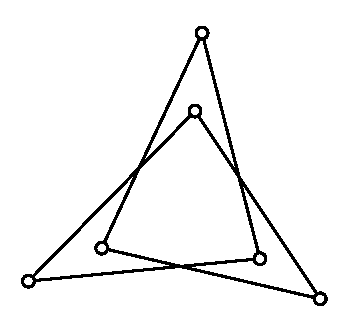
\includegraphics[width=27mm,angle=0]{pics/lomannaya}
\vskip-4mm
\end{wrapfigure}

На районной олимпиаде не решаю одну задачу, 
до сих пор стыдно.
Надо было предъявить пример замкнутой ломанной линии из 6 звеньев как на картинке ---
каждое звено пересекает ровно одно другое.
(Остальных задач опять не помню; как уже говорил, помню только те, что не решил.)

На городской тур я не прохожу
--- мою работу, наверное, теряют,
но Елена Артуровна договаривается, чтобы мне разрешили участвовать.%
\footnote{Тони на городской тур прошёл.
Последний раз когда я его видел,
он вдруг обвинил меня в том, 
что я предлагал ему денег за пригласительный билет на городскую олимпиаду.
В таком действии не было никакого смысла, ведь мне бы пришлось выступать как Антон Липкин.
Однако, возможно, это правда --- я точно помню, что на городской тур мне хотелось попасть параноидально.}
Я получил какой-то похвальный отзыв.
На вручении впервые увидел Сашу Гиля (о нём читай ниже), он с чем-то поздравлял учительницу своего кружка (видимо, Марию Юрьевну Филипову).
С ним был ещё один кружковец, по-моему, Фикс.

\paragraph{Психолог.}
Школа.
Я разговариваю с милой тётей%
\footnote{Потом узнал, что доверительная беседа --- это необходимый компонент в психологических исследованиях.
Надо сказать, что у тёти получилось очень натурально.}
и она предлагает пройти психологический тест.

Надо было добавлять карточку с геометрической картинкой к данному набору, чтоб подтвердить закономерность.
Задания сначала простые, но вдруг некоторые становятся сложноватистые;
я торможу, мой мозг вскипает.

Вызвали к психологу мою маму.
Ей объяснили, что со мной будет сложно и у меня не будет ни своей семьи ни детей.

\paragraph{Транспорник.}
Видимо в это время меня отправляют в удивительный пионерлагерь от трамвайно-троллейбусного парка нашего района.
(Мой отчим какой-то начальник в ЛенАвтоТрансе.)
Маленький лагерь, всего три группы: старшие, младшие и детдомовские.

В лагере нет формализма, территория строго не ограничена, можно уйти гулять по деревне или воровать яблоки по окрестностям.

Детдомовские как большая семья --- заступаются друг за друга круче, чем брат за брата.

Воспитатели --- народ молодой и душевный.
Директора лагеря звали Семён Ефимович.
Раз в месяц он произносил нараспев речь на День зарничника:
«Где бы вы ни были, вы должны помнить --- зарничник это воин, который в любую минуту может приступить к защите своей родины.
Юные ленинцы, в борьбе за дело Коммунистической партии Советского союза, будьте готовы» --- «Всегда готовы! Ура! Ура! Семёну Ефимычу».
Зарница --- это такая военная игра: в основном все бегают по лагерю с палками и говорят «пиф-паф»,
но  ещё привозят солдат, и они стреляют холостыми из автоматов, а
ещё дают в противогазе побегать в дыму.

У лагеря есть своя песня с бодрым мотивчиком, мы её поём в строю;
она мне до сих пор очень нравится.

\begin{verse}
Наши отцы спозаранку,
\\
С первой зарёй встаю-ют,
\\
И за баранкой и за баранкой
\\
Вахту свою несу-ут.
\\
\ 
\\
Транспортник, лагерь весёлого де-етства,
\\ 
\qquad ля-ля-ля-ля-ля-ля.
\\
Транспортник, солнцем и дружбой согре-етый,
\\ 
\qquad ля-ля-ля-ля-ля-ля.
\\
\ 
\\
Здесь мы набираемся здоровья-силы!
\\
Нашим воспитателям ура-спасибо!
\\
\ 
\\
Транспортник, транспортник --- самый лучший ла-агерь.
\end{verse}

По вечерам, один пионервожатый рассказывает истории, разное удивительное, в том числе о романе «Мастер и Маргарита» Булгакова.
Я зачем-то рассказываю стихотворение Пушкина «Анчар». 
Реакция у пацанов удивительная, всем нравится, читаю его чуть не каждый вечер.

Я сказал этому пионервожатому, что мне нравится геометрия.
Он меня спросил, что будет с теоремой Пифагора на сфере.
Я задумался, как считать углы и расстояния на сфере. 
Решил что надо смотреть на углы между хордами и длины хорд.
После этого естественно заявил, что теорема Пифагора останется прежней, но какие-то смутные подозрения, что это не так, оставались.

Позже, приехав домой я сказал про это отчиму.
Он воткнул три спички в горбушку батона и сказал, что надо мерить длины натянутых между ними нитей --- спасибо ему за это.



\paragraph{8-й класс.}
Проходит лето. 
Я вернулся из пионерлагеря.
По каким-то кривым наводкам нахожу Елену Артуровну.
Она живёт в общаге, вид у неё очень жалкий --- это всегда так.
Спрашиваю, когда начнётся кружок.
Она говорит, что нескоро,
выдаёт мне каких-то задачников, чтоб я не скучал,
и рассказывает, что летом преподавала в летней математической школе от Дворца Пионеров и что там очень сильные дети.
Мне становится обидно --- чего это она меня туда не позвала.

\paragraph{Программа «Время».}
Отчим заставляет меня каждый вечер смотреть программу «Время».
Ничего не понимаю, зато перед сном из головы выходят 
заблудившиеся там казённые фразы, окончательно потерявшие всякий смысл.

\paragraph{Дворцовский кружок.}
В начале третьей четверти,
я нахожу этот самый кружок от Дворца пионеров (мне помогают мама и отчим) и меня приглашают посетить занятие на пробу.
Я одеваюсь в свой приличный костюм --- пиджак-рубашка-брюки, может, даже жилетка.
Прихожу на занятие раньше времени, рассматриваю стенгазету с картинками типа Эшера.
Там есть уголок с объявлениями, где написано, что некий Саша Гиль выздоравливает, его температура такая-то и чего-то ещё.

Усаживаюсь на первый ряд слева.
Заходят кружковцы.
Чувствую небольшую волну --- наверное я занял чьё-то место.
Все рассаживаются по двое за парту --- я один один.
Начинается занятие, обсуждается задача, я вроде понимаю как её решить.
Вместо того, чтоб сказать это преподавателю, оборачиваюсь и говорю это мальчику позади меня 
(Серёже Ягунову).
Он меня слушает и говорит, что в этом решении я пользуюсь аксиомой выбора, а этого делать нельзя.
Я не знаю, что такое аксиома выбора, мне кажется, что все вокруг страшные снобы, и я решаю больше сюда не ходить.

\paragraph{Диалектика.}
В школе меня бьёт один парень, назовём его Кузьмой --- не помню, как его зовут.
Мне это сильно надоедает.

В это время на уроках обществоведения мы проходим диалектику.
В частности, нам объясняют следующую простую схему с четырьмя понятиями;
если натренироваться она применима практически везде.
В любой \so{системе} есть \so{противоречия} и со временем они только усиливаются это приводит к \so{конфликту} и его разрешению.
В результате получается новая система с новыми противоречиями.
Но для конфликта нужен \so{толчок}, 
и без него прогнившая система может долго сохраняться.
Однако, в сильно прогнившей системе толчок может быть произвольно невинным событием.

Пытаюсь применить диалектику на практике:
(1) выделяю систему --- я и Кузя;
(2) противоречия на лицо --- мне сильно не нравится, что он меня бьёт;
(3) для разрешения конфликта нужно организовать толчок.

Мы в этом году учили странный предмет --- что-то типа «Практика и гинекология семейной жизни».
По-моему, мы были первыми и почти последними, кому такой предмет преподавали.
Вместо учебника была брошюрка страниц на 20, где объяснялось, откуда дети получаются, и ещё просили не трахаться до поры до времени.

Моя брошюрка была разрисована всякими неприличностями, а у Кузи была аккуратненькая.
Совершенно случайно кто-то сзади просит меня передать Кузе его брошюрку.
Я её быстро меняю на свою, и толчок организован.
Как раз конец урока, Кузя не разобравшись, бьёт меня по роже сильно,
я пытаюсь тоже махать руками, но шансов мало.
Иду в туалет сполоснуть лицо и вижу что мой нос свёрнут на сторону.

Еду в травмпункт, родители на работе --- ещё не в курсе.
Из травмпункта меня отправляют в больницу Раухфуса,
где здоровая докторша каждый день кладёт меня на операционный стол
и потихоньку вправляет мне нос.
Она упирается в мой нос большими пальцами обеих рук, и раздаётся хруст где-то в моей черепушке.
После этого я смотрю в зеркало и пытаюсь понять, насколько нос стал прямее.
Через две недели мой нос почти прям.
Но я вдруг понимаю, что в мире нет людей с прямыми носами:
у всех дикторов телевидения нос слегка вбок, а о людях вокруг и говорить не приходится.

\paragraph{Саша Гиль.}
В больнице, на соседней койке лежал парень,
мы слегка подружились, рассказываем друг другу о том о сём.
Я рассказываю про тот самый кружок и
чувствую с его стороны волну интереса.
Это тот самый Саша Гиль, с тех самых пор мой лучший друг.
В больницу приходит МЮФ (Мария Юрьевна Филина) 
преподаватель того самого кружка,
приносит нам задачник по планиметрии, по-моему, Прасолова.
Мы с Сашей прорешали в нём все задачи.

После больницы я вернулся в кружок.

\paragraph{Диалектика работает.}
Кузя сильно испугался последствий; обходит меня стороной.

Так прошёл один из основных поворотов моей жизни;
забавно, что сломанный нос в этом помог.
Всё это случилось зимой, в начале третьей четверти.

Кто-то в классе сочинил про эту историю поэму, помню только пару строк: 
«На пол пути к победе, Петрунину сломали его большой учёный нос.»

\paragraph{Книги.}
Часто копаюсь в магазине строй книги на Гражданском проспекте.
«Библиотечка квант», «популярные лекции по математике» и всё такое.
Из того, что смог прочитать и понять, 
самой сложной для меня оказалась книжка Хинчина «Три жемчужины теории чисел».
Понял всё, но понравилась только теорема Ван-дер-Вердена про то, что если натуральный ряд раскрасить в конечное число цветов, то можно найти произвольно длинную арифметическую прогрессию одного цвета.
Решение сильно геометрическое.

%\paragraph{Число \emph{e}.}
%Однажды решил просуммировать обратные к факториалам на калькуляторе; ряд очень быстро сходится.
%Влад Казначеев (другой кружковец) увидел, что это почти в точности $e-1$, совпадений быть не может.
%До этого момента я вообще не знал, что это за число, да и после долго не знал.

\paragraph{Головоломки.}
Почему-то помню задачу о расстановке 8 ферзей на шахматной доске так, чтоб ни один не бил другого.
Провозился с ней пару дней, нашёл расстановку и тут же забыл.
С тех пор каждый раз трачу пару часов, чтоб восстановить решение. 
Запомнить так и не смог.

Где-то в это время мне достаётся кубик-рубик.
До сих пор горд тем, что придумал алгоритм самостоятельно.
При этом сам придумал сопряжение и коммутатор из теории групп.

\paragraph{$\bm{2{\cdot}\pi}$.}
Меня сильно волнует вопрос, почему угол вокруг точки всегда $2{\cdot}\pi$.
(Точной формулировки вопроса придумать не могу.)
Узнав о геометрии Минковского\footnote{То есть геометрия плоскости с метрикой, определённой нормой.} я с радостью обнаруживаю, что угол может принимать любое значение от $6$ до $8$.
К сожалению, плоскость становится менее симметричной.
Начинаю увлекаться геометрией Минковского, обобщаю для неё почти всё, что я знаю про фигуры постоянной ширины.

Потом вдруг решаю, что правильные многогранники вполне себе симметричны, и у них значение угла не  $2{\cdot}\pi$.
Почему-то меня это тут же успокаивает.

\paragraph{Городская олимпиада.}
В кружке не блещу, 
но по странному стечению обстоятельств выигрываю городскую олимпиаду по математике.
После окончания олимпиады выхожу уверенный в том, что я хуже всех.
Кружковцы мне говорят, что всё наоборот.
Я ловлю какого-то члена жюри\footnote{Через пару лет я знакомлюсь с этим человеком, 
это Нецветаев Никита Юрьевич --- умный хамовитый алкоголик-математик.}  
в коридоре и спрашиваю, какой лучший результат.
Он говорит --- «выиграл какой-то Петрунин».
(Выходит, что в кружке меня натренировали за пару-тройку месяцев.)

С этого дня решил, что я математик.
Поток начинает меня толкать в ту сторону, где я сейчас.
Иногда брыкаюсь, но остаюсь математиком.

На одну задачу от меня отстал Глеб Калинин, а все остальные на две.
Параллель на год старше выступила хуже нас
(надо исключить Ольгу Леонтьеву --- бесспорного лидера параллели, которая допускается до Всесоюзной олимпиады за прошлые достижения).  
Мы с Глебом едем на Всесоюзную олимпиаду.
На сборах в пионерлагере Зеркальном, 
знакомлюсь с этой самой Ольгой; у неё прозвище Курица.
Шалопайка,
в меру упитанная и весёлая.
Мы всегда вместе, с ней легко, меня иногда зовут «Курёнышем».
Потом она в меня влюбится.
Я влюбиться не успею, но больше об этом писать не буду.

Руководит нами товарищ ВЛИУСЕР (Всеми Любимый И Уважаемый Сергей Евгениевич Рукшин).
Первый раз я увидел его перед началом городской олимпиады.
Он вышел, объяснил нам правила игры.
Я почему-то обратил внимание,
что у него сиськи
почти как у тёти.
Он сказал несколько слов, 
но при этом успел выпереться.
Трудно объяснить как, если с этим не сталкиваться, вроде математическая элитность близко лежит.

\paragraph{Учительница английского.}
С английским проблемы.
Мама сватает меня на дополнительные занятия с моей учительницей.
Я оказываюсь у неё дома.
Она меня тренирует, прагматично и в меру успешно.
Пожилая женщина, помню, что обувь у неё была с коррекцией длины ноги --- одна нога была сантиметров на десять короче другой.

Вдруг я увидел, что эта учительница вполне себе человек, вполне симпатичный.
До этого она воспринималась мной как говорящая мебель.
У неё есть пианино и метроном в маленькой квартирке у Ольгинского пруда.

\paragraph{Ашхабад.}
Всесоюзная олимпиада проходит в Ашхабаде.
Мы летим туда на самолёте, живём в школе.
Из местных достопримечательностей помню только старика в халате.
Спросил можно ли его сфотографировать, он, по-видимому, сказал «нет» на местном языке.
Почему-то жалко, что не попробовал местного плова.
Наверно был вкусный, но я видел, как его готовили --- повара не выглядели сильно чистыми.

\paragraph{Фотка.} На фотке я в матлагере под лесенкой в наш корпус; возможно, лето 1983-го года.

\begin{figure}[h!]
\centering
\begin{lpic}[t(-0mm),b(-0mm),r(0mm),l(-0mm)]{pics/uzel(0.8)}
\end{lpic}
\end{figure}

\paragraph{Четырёхугольник.}
В матлагере попадается такая задача.
Рассмотрим четырёхугольник с жёсткими сторонами и шарниром в каждой вершине;
предположим мы начинаем его шевелить, увеличивая, скажем, сумму двух противоположных углов (обозначим её $\alpha$)
и смотрим как при этом меняется площадь.
Надо доказать, что площадь увеличивается пока $\alpha<180^\circ$ и уменьшается при $\alpha>180^\circ$.
Решается простым подсчётом,
но я чувствую, что мне это ещё пригодится --- странное чувство, тяжело отделаться.
Действительно пригодилось лет через 10 ---
если бы не пригодилось, то, наверное, забылось бы.%
\footnote{О том я написал статью \emph{Area minimizing polyhedral surfaces are saddle} для Monthly.}

\paragraph{Признак Лобачевского.}
В том же лагере, иду из столовой и догадываюсь почему ряд $1+\tfrac{1}{2^s}+\tfrac{1}{3^s}+\dots$ сходится при $s> 1$ 
и расходится при $0\le s\le 1$.
В доказательстве пользуюсь тем, что 
$$\tfrac n{(2{\cdot}n)^s}
\le \tfrac1{(n+1)^s}+\dots+\tfrac1{(2{\cdot}n)^s}
<\tfrac n{n^{s}}.$$
Не великое достижение, особенно если принять во внимание, что доказательство то же, что и для гармонического ряда  $1+\tfrac{1}{2}+\tfrac{1}{3}+\dots$, которое я знал.
Но это был первый случай, когда я понял, что грубая оценка может дать точный результат;
поэтому запомнил.


\section*{Школа 239}
\addcontentsline{toc}{section}{Школа 239}



\paragraph{«Быть или не быть».}
Кружок становится половиной класса «9-4» 
в «тридевятой» школе.
Этим летом я иду подавать туда документы.
Чего-то жду в коридоре, читаю стенгазету для выпускников, что-то вроде такого:
\begin{verse}
...эта задача посложней задачи Гамильтона «быть или не быть»;
у нас задача «кем быть, каким быть»...
\end{verse}
Я не так давно прочитал  «Теорию графов» Оре%
\footnote{На всякий пожарный --- книжка посредственная.},
там обсуждался вопрос существования Гамильтонова цикла в графе.
Действительно вопрос «быть или не быть»,
и не существует быстрого алгоритма для отыскания ответа.
Стою и думаю, что газета написана для всех --- круто, в этой школе все знают про Гамильтоновы циклы.%
\footnote{Очевидно, там было написано «Гамлета», а не «Гамильтона», но о Гамлете я не знал ничего.}

\paragraph{Две собственных задачи.}
По-видимому, этим летом, в обычном (не математическом)
пионерлагере я думаю о том, что во всех олимпиадных задачах
есть большая подсказка, состоящая в том, что решение есть и оно простое.
Пытаюсь придумать задачи сам.

Первая была такая: найти плоскую фигуру наименьшей площади,
которой можно накрыть любую фигуру диаметра 1.
Тыркаюсь, понимаю, что достаточно накрыть все фигуры постоянной ширины 1, но решить не могу.
В конце лета, уже в мат-лагере, узнаю от сокружковцев,
что это так называемая \so{задача Лебега}, и она до сих пор не решена.

В другой задаче надо было определить, можно ли из данной расстановки фишек на бесконечной шахматной доске 
получить другую (данную) расстановку, если позволяются только ходы как в уголках 
--- фишка может только перескочить через фишку на одной из четырёх соседних клеток.
Эту задачу я решаю и ответ получается похожим на алгоритм, 
совсем не олимпиадный.

Конечно, количество фишек в двух расстановках должно быть одинаковым.
Очевидно, что при каждом ходе фишки не меняют чётность своих координат.
Поэтому и число фишек с координатами чёт-чёт, чёт-нечет, нечет-чёт и нечет-нечет тоже должно быть одинаковым.
Оказывается, что если до любой клетки доски можно допрыгать, начиная с каждой из расстановок, то этих четырёх равенств достаточно.

Чтобы найти множество досягаемых клеток, нужно начать закрашивать клетки по такому правилу:
сначала закрасить все клетки с фишками.
Далее если две соседние клетки закрашены, то следует закрасить все клетки на образованной ей прямой.
Повторять процесс до стабилизации.
Легко видеть, что в конце мы закрасим либо всю доску,
либо набор прямых, из которых нет соседних параллельных, плюс, ещё быть может набор изолированных клеток.

Помню, что я полностью решил последний случай, но ответ уже не помню.
Пишу, чтоб похвастаться --- сам придумал задачу для исследования и сам с ней справился --- важный шаг.

\paragraph{239.}
Началась школа.
По дороге в школу американское консульство.
Огромный флаг и страж в будке.
Можно подойти к стенду и почитать, что там написано.
Меня одновременно удивляет, что в нашем городе может вот так безнаказанно развеваться американский флаг,
и то, что никакой антисоветчины на стенде нет.

Раз или два в неделю идём пешком по 
Литейному в кружок во Дворец пионеров.
Никакой красоты не замечал.
Городские красоты заметил уже после того, как пожил в других местах.
Я вообще мало чего вокруг замечал.
Были исключения --- места, которые я знал очень хорошо, например, парк Лесотехнической академии.

\paragraph{Учителя.}
Учителя начинают принимать очертания людей, 
не все конечно.

\begin{wrapfigure}{o}{50mm}
\vskip-4mm
\centering
\includegraphics[width=49mm,angle=0]{pics/kuksa}
\end{wrapfigure}

{\sloppy 

Учитель математики --- \so{Кукса Николай Моисеевич} (фронтовик-подводник),
относится ко мне почему-то очень по-доброму.
Иногда даёт мне какие-то глобальные жизненные советы, 
смысл которых я уловить не могу, хотя очень хочу.
Он что-то пишет на доске и бубнит под нос,
его почти никто не слушает.
Тренирует нас к поступлению,
даёт типовые задачи с подвохом.
Если кто-то попался, говорит: «Спасибо за покупку!».

}

«Пиначет» --- \so{Михайлов Михаил Васильевич} --- учитель истории, пиджак на майку
(в эти времена это знак пьющего человека).
Огромный нос и непременно палец в носу или около.
Ничему меня не научил, но симпатяга.

\begin{figure}[!ht]
\begin{minipage}{.49\textwidth}
\centering
\includegraphics[scale=.5]{pics/pinachet}
\end{minipage}
\hfill
\begin{minipage}{.49\textwidth}
\centering
\includegraphics[scale=.5]{pics/slutzkij}
\end{minipage}
\end{figure}

\so{Слуцкий Юрий Лазаревич} --- учитель физики.
Требовательный педант.
Шутит сухо, всегда с серьёзным лицом:
\begin{verse}
«Дети, надо учить уроки, другого метода выучить физику я вам предложить не могу».
\end{verse}
От него я узнал, что такое физическая интуиция;
наверно, лучший школьный преподаватель, который меня учил.%
\footnote{На встрече класса через 20 лет о Слуцком говорят только плохо.} 
Помню, что меня поразила задача про угол между тремя плёнками двойного пузыря.
Я сразу решил её физически, потом стал прикидывать, как решение можно записать математически правильно,
и удивился количеству возникающих сложностей.%
\footnote{До конца эти сложности тогда не понял --- задачу о двойном пузыре сформулировали в 1991, а решили в 1995.}

Физику преподают очень хорошо.
У нас есть лабораторные занятия.
Помню один опыт по определению скорости электромагнитных волн (то же, что скорость света)
---
полкилометра провода и осциллограф,
надо мерить отставание эха периодического импульса.

С английским огромные проблемы.
Сдаю зачёты, заучивая наизусть текст и перевод.
Учитель английского, «Лёлик» --- \so{Эйделькинд Леонид Михайлович}, фронтовик,
относится ко мне очень хорошо, 
может просто так, а может потому, что дружит с Куксой.
Всегда всем и себе улыбается.
Видел его без улыбки один раз,
когда Алёша Гуревич (или кто-то другой, кто стоял рядом) 
чуть не проломил стену в его кабинет.

\begin{figure}[!ht]
\begin{minipage}{.49\textwidth}
\centering
\includegraphics[scale=.5]{pics/eidelkind}
\end{minipage}
\hfill
\begin{minipage}{.49\textwidth}
\centering
\includegraphics[scale=.5]{pics/lebedeva}
\end{minipage}
\end{figure}

Пока учился, мне была симпатична учительница литературы, 
\so{Лебедева Янина Максимовна} --- ухватки генеральши.
В основном она лечила нас от «комплекса полноценности» (её термин).
По прошествии лет, она вызывает у меня скорее неприязнь.
В школе я не понимал, что по умолчанию заслуживаю уважение, и
в учительском хамстве видел скорее силу, чем преступление.

\paragraph{Начала анализа.}
Нас не учили по-настоящему анализу ни в кружке ни в школе.
Среди кружковцев пользоваться анализом считалось чем-то некрасивым.
Скажем, если кто-то решал задачу на минимум с использованием производной, то его заставляли доказывать все рутинные утверждения и представлять определения ---
обычно находили места к которым можно придраться, и кружковцу приходилось искать элементарное решение.

Получилось так, что анализ я не учил,
а придумал сам под большим давлением извне.
Помню, когда придумал, что производная --- это тангенс угла наклона касательной.
Был под впечатлением пару дней.
Это оказалось мостиком, по которому разрозненные идеи в моей голове вдруг стали общаться между собой.

Я придумал доказательство поризма Понселе, построив функцию на внешней окружности, такую что её интеграл по любой дуге, отсекаемой хордой касательной к внутренней окружности постоянен.

Другой пример --- доказательство того,
что если точка $M$ минимизирует сумму минимумов расстояний
\[\min\{A_1M,B_1M\}+\dots+\min\{A_nM,B_nM\}\]
для различных точек $A_1,B_1,\dots,A_n,B_n$, 
то
\[A_iM\ne B_iM\]
для любого $i$.
На эту тему я написал работу в школе, 
был этим взволнован и понимал, 
что этот метод (по сути применение производной) имеет массу других приложений.
Я показывал это старшим товарищам и видел недоумение на их лицах.
По-видимому, они не верили, что я могу не знать анализ.
(Сейчас я бы тоже недоумевал --- от девятиклассника ожидается чего-то большего.)

\paragraph{Вершины куба.}
Проделав нехитрый подсчёт, понимаю, что если вписать куб в $n$-мерную сферу, то при больших $n$ вершины куба становятся всё более плотными на сфере.
Это произвело на меня неизгладимое впечатление. 
Наверное первый раз почувствовал, что многомерный мир сильно другой.

\paragraph{Минск-22.} 
У нас в школе стоит электронная вычислительная машина «Минск-22»
занимает один кабинет.
Учим язык Алгол.
Программы сначала пишем от руки, потом вбиваем на перфораторах (ими уставлен отдельный кабинет).
Перфоратор похож на печатную машинку, но выдаёт ленточку с дырочками.
Ленточку надо засунуть в щёлочку. 
Она мгновенно проскакивает и выдаёт распечатку твоей программы и сообщение об ошибке.
После этого свою ленточку можно опять засунуть в перфоратор, забить ошибки пустым символом (он включает все дырочки) и, может быть, подклеить исправление.
Мне ни разу не удалось написать работающую программу.

\paragraph{Общество «Тензор».}
Меня с Серёжей Ягуновым назначили сопредседателями школьного математического общества под названием «Тензор» (а может мы были председателями в разные времена --- неважно).
Что такое тензор, я не знал, и это меня немного угнетало;
знал только, что это продолжение цепочки скаляр --- вектор --- матрица.

Мы договорились только об одной серии лекций, прочитанной нам Иваном Борисовичем Фесенко.
Лекции были по $p$-адическим числам; 
рекламный плакатик (с головами с острова Пасхи) нарисовал для этого случая Саша Гиль.
Лекции оказались очень полезными.

Ещё я отличился защитой Китайской Народной Республики.
У общества «Тензор» была своя стенгазета, к ней я не имел прямого отношения.
В разделе юмора я увидел шутку про новый вид оружия --- столько-то миллионов китайцев становятся на окружность, забираются на табуреточки и прыгают с них одновременно вызывая волну, приносящую гибель и разрушения в центре окружности.
Это была подпись под забавной картинкой с китайцами на табуреточках.
Мы это прочитали с Серёжей.
Мне показалось, что так нехорошо китайцев обижать.
Серёжа меня поддержал, я снял газету и высказал это учительнице по вычислительной математике --- она отвечала за общество.
Эту шутку залепили другой и повесили газету назад.

Помню смешанное чувство --- я поддаюсь порыву, немного переживаю, что неправ и всё-таки делаю.
Чуть позже мне было стыдно за эту выходку, но вида не подавал.
Ещё чуть позже я понял, что сделал всё правильно.
Наверно, подобные чувства часто испытывали партийные активисты, но мне довелось только раз.

\paragraph{День победы.} 
Всей школой идём по набережной, там народное гулянье, сильно пахнет весной.
В компании помню только Стаса Смирнова.

Набережная Кутузова, рядом с Литейным мостом.
Окно на первом этаже открыто,
там сидит забавный чувак, инвалид, он играет в шахматы с прохожими.

Узнав, что мы математики, просит решить для него дифференциальное уравнение.
Мне дико хочется ему помочь, но я не понимаю его обозначений.
(Да и куда мне, я дифференциальных уравнений никогда не решал.)
Стас берёт бумажку и обещает помочь.

Этот кусочек памяти похож на сон, 
тот самый, который хочется остановить и иногда туда можно вернуться.


\paragraph{Сборы.} На всесоюзной олимпиаде выступаю посредственно,
наверно кое-как вхожу в десятку.
Обидно, что на всех всесоюзных есть хотя бы одна задача,
которую я решаю поняв условие неправильно --- не дочитав до конца условие, придумываю своё и пытаюсь решить.

Тем не менее я прохожу на сборы.
Нас, человек 40, тренируют для международной математической олимпиады;
из них отберут 10, остальным сидеть на скамейке запасных, за то в универ без экзаменов.
Впопыхах вступаю в комсомол, старшие товарищи объяснили, что иначе шансов нет.

Сборы я не прошёл.
Мне казалось, что это случилось из-за того, что нас заставляли каждое утро бегать по мокрому снегу.
У меня не было подходящей обуви, и я всё время болел.
Вдобавок задачи на сборах были не вполне олимпиадные;
больше проверяли, что мы владеем техникой.

Помню одну устную задачу, которую я криво решил.
Надо было доказать, что инверсия пространства переводит окружности в окружности.
Очевидно ожидалось, что я воспользуюсь тем,
что окружность --- это пересечение двух сфер.
Я же доказывал, что образ окружности --- это эллипс,
и потом доказывал, что у него равны полуоси.
Сбило то, что как раз недавно читал где-то про шары Данделена.

По часу в день была
беседа с милым КГБистом.
Он нас спрашивал провокационные вопросы
и смотрел, как мы выкручиваемся, 
чтоб попасть за границу.
По-моему, эти занятия никакой роли не играли,
как и утренние пробежки по мокрому снегу.

Я очень хотел на международную олимпиаду и сделал максимум, чтоб не пролететь,
пролетел и расстроился.%
\footnote{Позже я придумал принцип: в таких случаях не прогибаться.
Если выгорит, то в двойне приятно --- если нет, 
то  можно считать, что не получилось потому, что не прогнулся.}

\paragraph{Олимпиадные задачи.}
Под конец школы просматриваю олимпиадный задачник.
Ощущение, что задачи разбиваются на штук 7 типов,
к каждому есть потёртая отмычка в кармане,
иногда надо немного поднапрячься и вскрываю.
Полное отвращение к олимпиадной деятельности.

Под конец школы Рукшин берётся за моё образование.
(Возможно потому что в спортивной математике я пролетел.)
Он меня снабжает сначала книжкой Бляшке «Круг и шар»,
потом
книжкой Рудина «Основы математического анализа».
После того как прочитал, дал мне книжку Натансона «Теория функций вещественной переменной».
Благодаря книжке Бляшке я понял, зачем нужны компакты;
до него я думал, что люди говорят «компакт» когда им лень говорить «замкнутое ограниченное множество Евклидова пространства».
Очень нравится Рудин.
Начинаю видеть красоту в больших формах.

Рукшина часто характеризуют как тупого олимпиадного тренера.
Это не так, он учит разумным вещам, когда видит что время пришло.
Я~помню несколько случаев, когда Рукшин «закидывал удочку» ---
проверял, есть ли интерес к чему-то вне олимпиадной тематики.
(Сказанное не отменяет то, что Рукшин говнюк, смотри ниже.)

\paragraph{Уникальносоставленные фигуры.}
Мы с Рукшиным пишем статью,
время такое, нет ещё ни TeX-а ни компутеров.
Рукшин надо мной конкретно издевается,
видимо думает, что учит меня писать.
Очевидно, что я писать не умею, но он тоже не умеет учить.
Почему-то помню одну свою описку: «Пусть $F$ --- выпуклая точка».
Приходится бесконечно перепечатывать подклеивать, разрезать и переклеивать.
Оконченную статью теряет Александр Данилович Александров.%
\footnote{Вместо неё ВЛИУСЕР печатает непонятно зачем сильно частный случай.
Я по молодости не перечу.
За эту статью мне до сих пор стыдно. 
Радует только то, что стала она библиографической редкостью.
Имел глупость спустя много лет переписать статью; послал в «Математическое просвещение».
ВЛИУСЕР её подпортил, и она была напечатана в этом виде.
Потом он ещё напечатал укороченный вариант статьи без моего ведома, включив меня как соавтора («Элементарная характеризация уникальносоставленных выпуклых фигур.» --- 2006).
Смотри мораль от моего дедушки: не имей дело с дураками.}

Писать статьи получилось очень не сразу.
Первую мою статью\footnote{«О триангуляции согласованной с покрытием.» Украинский геометрический сборник.
№ 35 (1992), 110---114.} за меня переписал Виктор Абрамович Залгаллер.
Потом статьи писал Гриша Перельман.

\paragraph{Контактное число.}
Приблизительно в это же время я догадался, что контактное число у $n$-мерного шара не превосходит контактного числа любого $n$-мерного тела;
это было частичным решением задачи, которую я увидел в книжке «Проблема тринадцати шаров» Яглома.\footnote{Много лет спустя узнал, что задача была решена существенно раньше выхода книжки Яглома: C.
Halberg, E.
Levin, E.
G.
Straus.
“On contiguous congruent sets in Euclidean space.” Proc.
Am.
Math.
Soc.
10 (1959), pp.
335--344.}


\paragraph{Кирилл и Мефодий.}
Перед выпускным экзаменом по русскому языку и литературе забежал в Спасо-Преображенский собор и поставил свечку к иконе Кирилла и Мефодия --- так мама научила.
Купил свечку, спросил у продавщицы, где икона, поставил и убежал.

Чувствовал себя весело и странно --- первый раз зашёл в церковь не из пустого любопытства, а как бы по делу.
За экзамен получил 4 балла --- на лучшее я и не рассчитывал.

\section*{Политех}
\addcontentsline{toc}{section}{Политех}

\paragraph{Под гипнозом.}
Закончил школу.
Как под гипнозом поступаю в Политех.
На меня поднадавила мама, объяснила, что математика из меня не получится и мне лучше идти учиться поближе.
В добавок, у меня случился нервный срыв с повышенной температурой и ослаблением воли.
(Воли у меня и в нормальном состоянии почти не было.) 

\paragraph{Задача Эрдёша --- Турана.}
В конце школы придумал себе такую задачу.
Доказать, что если $A\subset\mathbb{Z}_{3^n}$ не содержит арифметической прогрессии длиной три, тогда в $A$ максимум $2^n$ элементов;
то есть самое лучшее, 
что можно придумать, это  взять в $A$ все числа из $\mathbb{Z}_{3^n}$, 
которые записываются без нулей в троичной системе.

Откуда-то берётся уверенность, что это правда.
Бьюсь изо всех сил, думаю про это всё лето пока поступаю в Политех.
Потом нас, поступивших, посылают в колхоз.

Возвращаюсь из колхоза, всё, что я думал про задачу, полностью стёрто из головы.
Спрашиваю народ, ответа не нахожу.
Странным случайным образом узнаю,
что это вопрос Эрдёша --- Турана;
в 42-м к нему нашли контрпример Салем и Спенсер.
Их статью я не могу отыскать в библиотеках, но есть более поздняя статья. 
За ней я еду в противоположный конец города, в сторону станции «Звёздная».

Прочитал при полном незнании английского.
Решение геометрическое, по сути используется то, 
что многомерная сфера пересекается с прямой не более чем в двух точках;
значит, если $A$ есть пересечение сферы и целочисленной решётки в евклидовом пространстве,
то в $A$ нет арифметических прогрессий длины три.
Остаётся правильно подобрать радиус сферы и размерность пространства,
так чтоб $A$ было большим,
но всё ещё его можно было 
линейно отобразить в $\mathbb{Z}_{3^n}$, так чтобы новых арифметических прогрессий не появилось.\footnote{Видимо мне досталась статья Бехренда.
Повезло --- в статье Салема со Спенсером геометрией не пахло.}

В том колхозе со мной случилась забавная история. 
Я познакомился с милой девушкой, имени её не помню, полненькая и весёленькая, не питерская.
Однажды жжём с ней пол ночи костёр, 
под утро засыпаем, и нам снится одинаковый сон
про людей, которые закапывают клад где-то неподалёку.

\paragraph{Библиотека.}
В Политехе отличная библиотека, огромный читальный зал с высоченными потолками,
можно сравнить только с храмом (может переделана из церкви).
Копаешься в каталоге, заполняешь заявку, и через день или два получаешь книгу.
Читал всё по математике.
Помню древнюю книжку по «Высшей арифметике»,
в которой объяснялась коммутативность и ассоциативность умножения с помощью движений пространства --- крутили трёхмерную таблицу, заполненную единицами и считали по-разному их сумму.

По комбинаторной геометрии читаю всё, что могу найти.
Мне попадается книга страниц на 300,
в которой считается контактное число пентагона;
то есть решается вопрос сколько одинаковых правильных пятиугольников можно прислонить к такому же пентагону на плоскости так чтоб все пентагоны не имели общих внутренних точек.
Почему-то запомнился тираж: 500 штук.
Задача решается чрезвычайно занудными вычислениями, 
ещё и с привлечением компьютера.
До меня наконец доходит, что не вся комбигеометрия прекрасна.

Из хорошего, я прочитал там «Выпуклые многогранники» и «Внутренняя геометрия выпуклых поверхностей» Александрова.%
\footnote{Недавно Юрий Дмитриевич Бураго сказал, что Александров пишет так, что создаётся ощущение, что ты понимаешь, как он думает.
На мой взгляд, очень метко замечено.} 
Почему-то меня очаровали квазигеодезические.


Учат очень хорошо, но с причудами.
Очевидно, что программа не менялась лет двадцать,
например, натаскивают на эллиптические интегралы.%
\footnote{Этому можно учить только с одной целью --- проверить, что студент в состоянии выполнять данный алгоритм.
Недавно узнал, что до сих пор там этому учат, хотя уже тогда в этом не было никакого смысла.}

Запомнились лекции одного старенького инженера, к сожалению не помню имени.
Он приводил огромное число простых в исполнении, но не тривиальных инженерных решений.
Кое-что подобное мне до этого рассказывала мама.
От него я узнал про использование эвольвентного профиля в зубчатых передачах.
Простые механизмы позволяющие передавать движение между камерами с различным давлением, приёмы уменьшения вибрации в механизмах.
Красота этих решений до сих пор впечатляет, хотя ничего из этого мне не пригодилось.

\paragraph{Васильев.}
Линейная алгебра, 
геометрический подход, 
первый курс. 
Девочки плачут, ну а мне нравится.
Ведёт Васильев --- толстый, улыбчивый монстрик.
На экзамене я имел глупость заявить: «я знаю всё».
Он мне тут же предложил придумать, как брать экспоненту от матрицы.
Разумеется, этого в программе не было,
мне как раз хватило --- стал выпендриваться по-меньше.
(Выйдя с экзамена, догадался, что можно было бы воспользоваться рядом Тейлора, но уверенности не было.)

\paragraph{Мастеров.}
Статистическая механика и теория относительности --- отличные лекции, читает Вадим Фёдорович Мастеров.
Рассказывал нам про энтропию. 
В меня входило со скрипом, 
но вошло, держу в себе с удовольствием.

Заснул на лекции.
Проснулся под конец.
По моему всклокоченному виду было всё ясно.
(Может, я ещё и похрапывал во время лекции.)
Мастеров мне сказал --- «А Вы, молодой человек, сдаёте экзамен только мне».
Он не забыл --- сдавал ему --- сдал на отлично.

\paragraph{Контролёр.}
Еду в трамвае без билета,
появляется контролёр надо платить штраф.
Обычно в таких случаях я делаю ноги,
смотрю в глаза контролёру --- радужная оболочка одного его глаза разбита на два сектора разного цвета
120 и 240 градусов.
Обалдел на столько, что заплатил штраф.


\paragraph{Оля Митренина.}
Подружился с некой Ольгой Митрениной.
Она иногда подкармливала меня иностранным шоколадом и щебетала об иностранных книжках.
Я таскался за ней на продвинутый английский.
Ни черта не понимал, но преподавательница (Светлана Игоревна Горохова) была очень весёлая, и это как-то скрашивало время.

Оля умная и красивая.
Зимой ходит без шапки --- смотреть на неё холодно.
Искренне интересуется окружающими людьми.
Все юноши влюбляются и я не исключение; писать об этом не буду.

Как-то она мне показала своё стихотворение, мне оно дико понравилось.
Оказалось, что я его до сих пор помню:
\begin{verse}
Мой восемнадцато-белый малиновый сторож
\\
\qquad не знает когда мне придётся вернуться
\\
\qquad\qquad  и если проснуться,
\\
\qquad\qquad\qquad то будет ли сон мой неважно.
\\
Смотри, заколдованы сосны, бумажный,
\\
\qquad игрушечный снег их укроет,
\\
\qquad\qquad и бережно скроет последние тёмные пятна
\\
\qquad\qquad\qquad тихонько невнятно.
\end{verse}
Оно мне до сих пор нравится.
Очень возможно, что я в нём вижу больше смысла чем там есть.

Вот пара анекдотов, которые она рассказала про себя.
У неё дома варенье хранилось в двухлитровых банках,
иногда она его подъедала и, чтобы скрыть преступление, доедала банку до конца, мыла и ставила на полку.
Ещё в детстве она носила с собой набор на случай, если её занесёт в дикие места.
Кроме необходимых вещей для выживания там были стеклянные бусы и губная помада для обмена с аборигенами. 

Позже встретил её в окружении попов --- было её жалко.
Потом она (вроде) подалась в Суздальский раскол, но преподаёт лингвистику в универе.

У неё был Живой журнал (\texttt{mitr.livejournal.com}), можно было подсмотреть, чем и как жила.
Мне понравилась там пара мест:
Оля делится своими переживаниями, что её могут неправильно понять, и получает следующий ответ (проникнутый оптимизмом и знанием людей): «Вы не представляете как мало места занимаете в жизни других людей».
Ещё там была идея, что про любой день и час, когда можешь работать, лучше думать, что получил его взаймы.
(Почти согласен, ну уж точно не надо думать, что так оно и должно было быть и рассчитывать, что завтра будет также.)

Много позже мы с ней встретились, погуляли, поговорили ни о чём, и разошлись.

\paragraph{Одногрупнички.}
Из одногрупничков помню ещё Ильюшу Мазура,
Жеку П\'{о}дноса и Диму Ямпольского (Мича).

Мы идём по парку вместе с Ильюшей.
Нам попадается компания молодых людей КСПэшно-походного%
\footnote{КСП --- клуб самодеятельной песни; тяжело объяснить что это за люди; 
типа любители петь под гитару с сектантским блеском в глазах.}
типа.
На лицах единство.
Хорошие добрые ребята, 
но почему-то неприятно и почти страшно на них смотреть.
Удивительным образом независимо, мы думаем про них одно и то же,
наверно, поэтому этот эпизод запомнился.

Ильюша объяснил мне построение неизмеримых множеств ---
конструкцию Хаусдорфа.

Однажды мы бесились на крыше, и надо было идти на лекцию.
Решаю подшутить над Жекой --- запереть его на крыше.
Закрываю окно, 
его пальцы зажимаются рамой.
Он не кричит, вместо этого белеет на глазах.
Ничего не понимая, я давлю дальше на створку окна, 
пока не догадываюсь, что что-то не так.

\paragraph{Армия.}
Прошёл медкомиссию, иду служить в армию.
Тяжеленная сумка с математическими книгами.
Нас грузят в автобус у военкомата, отправляют в какой-то центральный военкомат.
Там нас делят на команды, и мы ждём сопровождающих.
Сидим в спортзале на полу до вечера, мою команду расформировывают, и я еду домой --- типа повезло.

\section*{ЛОМИ}
\addcontentsline{toc}{section}{ЛОМИ}

\paragraph{Малышев.}
Есть такой профессор Александр Васильевич Малышев. 
У него семинар по геометрии чисел.
Это такая наука про решётки, начинается с задачи Минковского про то, что выпуклая фигура площади $4$ симметричная относительно начала координат, обязана содержать целочисленную точку, отличную от начала координат.
Хожу, но практически ничего не понимаю.

Малышев меня снабжает книгой Реккеркеркера «Геометрия чисел».
Прочитал и вроде понял.
Малышев пьёт;
иногда в подпитом состоянии звонит ко мне и спрашивает, над какой задачей я сейчас думаю.
Однажды я ему сказал, что не уверен в том, что хочу заниматься геометрией чисел, и думаю заняться дифференциальной геометрией.
Запомнил его ответ: «Не нужно думать --- нужно просто решать задачи.»
Однажды он позвонил ко мне когда меня не было дома.
Мама сняла трубку,
он попросил сказать, какая книжка лежит у меня на столе.
На столе лежали «Автоморфные функции» Форда.
«Отличная книжка» --- говорит Малышев --- «но почему он такое старьё читает».

В это время я мог читать книги изданные до 1936 года.
Наверное, после этого книги становятся слишком сложными.
И «Автоморфные функции» Форда были очень понятно написаны и изданы ровно в 1936-м.
Ничего понятного на эту тему я больше не читал.

\paragraph{Бураго-старший.}
Юрий Дмитриевич Бураго нам читает дифференциальную геометрию в стиле Александрова.
Седловые и выпуклые поверхности,
теорема Топоногова, 
теорема Громова о компактности.
Меня постепенно затягивает.
При этом веду себя на лекциях по-свински;
мне интереснее всего подловить лектора на ошибке.
Очень понравилась теорема Шефеля про седловой график.

Юрий Дмитриевич --- старичок с женским голосом,
похож на доктора Верховцева из «Тайны третьей планеты».
Носит пиджак на пару размеров больше, чем нужно,
постоянно скошенный на один бок.
Нехватка лёгкости бытия --- во всём видит проблему и всегда готов объяснить её причину.
Разговаривает всегда в доверительном тоне,
как будто сообщает секрет.

\so{Анекдот.}
Встречаю Юрия Дмитриевича при входе в ЛОМИ.
Он берёт пару ключей на вахте.
Прежде чем зайти в свой кабинет, включает свет в соседнем.

--- Зачем?

Напротив ЛОМИ, через Фонтанку, расположен районный партком.
Тамошний народ приходит на службу утром и уходит вечером.
Им обидно, что институт математики почти не включает свет, и эта обида как-то проявлялась (не знаю как).
В результате Фадеев (директор института) выдал распоряжение: «Пришёл на работу --- включи свет соседу».

\paragraph{Залгаллер.}
В ЛОМИ рядом с кабинетом Виктора Абрамовича Залгаллера, есть шкафчик, наполненный им вырезками из  «Math\-em\-at\-ical Reviews».
Каждая вырезка аккуратненько наклеена на картонку, 
всё разложено по темам в коробочки.
Роюсь там часами.

Пару раз Залгаллер читает нам лекции вместо Бураго.
Рассказывает о применении комбинаторной геометрии:
вырезание нужных прямоугольников из данного,
нарезка древесины,
вырезание стелек в таких масштабах, 
что экономия одного процента стоит работы математического института.
Увлекательно рассказывает: 
рассказав о теореме, тут же рассказывает о том, как и кто её решил, 
рисует целую картину.

Залгаллер попросил меня посмотреть на работу какого-то математика из Калинина.
Мне дают отпечатанный на машинке тяжёлый труд.
В нём невозможно ничего понять, даже задачу, которую человек решает.
Долго пытаюсь найти в этом какой-то смысл,
потом начинаю читать подряд и на второй странице нахожу неверное утверждение.
Сообщаю об этом автору.
Он не исчез, приезжал в Питер раз в пол года и пытался со мной ещё побеседовать;
звонил домой и называл меня «Антоном Михайловичем».

Спросил у Залгаллера чтобы мне полезного почитать.
Он тут же вытащил статью (какой-то кривой заграничный скан) и просит меня в ней разобраться.
Сейчас понимаю: по-видимому, его попросили написать аннотацию для Mathematical Reviews, и он тут же нашёл, кому её сплавить.
Трачу на статью полгода, роюсь в том же Залгаллеровском шкафу.
Нахожу, что тот же результат был доказан Погореловым.
Сообщаю об этом Залгаллеру.
Он направляет в мою сторону своё огромное ухо. 
Слушает; потом говорит: «очень хорошо» и уходит --- видимо аннотацию уже писать не нужно.

Сдаю кандидатский минимум по английскому.
Должен привести профессора со своей кафедры.
Так получилось, что во время сдачи экзамена все были заняты, кроме Залгаллера --- он согласился прийти.
При этом Залгаллер не говорил по-английски;
читать, конечно, мог.

Экзамен состоял из двух частей: я должен был перевести текст из книжки Чигера и Эбина на русский,
преподавательница английского следила за языком, а Виктор Абрамович за смыслом.
Далее требовалось, чтобы мы обсудили что-то математическое друг с другом.
Тут Виктор Абрамович заявляет, что во время войны у него была выбита перепонка (начало войны, о том есть в его мемуарах) и грубые языки --- русский или немецкий --- он может воспринимать, а мягкие, типа английского, никак не может.
Девушка спросила несколько вопросов о войне, и на этом экзамен закончился.

(Кстати, вступительный экзамен в аспирантуру по английскому за меня сдал добрый Слава Матвеев.)

А вот анекдот, рассказанный самим Залгаллером.
Монастырь, какой-то праздник.
Народ в ожидании чуда, и сам Залгаллер заражается общим настроением.
Виктор Абрамович видит необыкновенно красивого монаха.
Просит разрешения его сфотографировать и получает ответ --- «Оставим память в сердцах наших».

\paragraph{Как я выбрал дифференциальную геометрию.}
Не мог понять, чем лучше заниматься --- 
геометрией чисел или дифференциальной геометрией.
Не находилось внутренних и чисто математических причин.
В конце концов, посмотрел на кафедру геометрии и кафедру теории чисел;
увидел, что в геометрии люди поживей и повеселей, и занялся дифференциальной геометрией.
Тогда мне казалось, что это глупый, почти слепой способ решения вопроса.
Теперь мне кажется, что это было одно из самых умных решений моей жизни.


\section*{Матмех}
\addcontentsline{toc}{section}{Матмех}

В конце первого курса пытаюсь перевестись на матмех.
Беседую в деканате с человеком по фамилии Ананьевский ---
такую фамилию трудно забыть.
Сообщает мне,
что у меня нет шансов,
но можно подать заявление, и мне непременно придёт отказ.
Я это и делаю.
После этого прошу поднадовить Александра Васильевича Малышева и меня взяли.
(За то ему большое спасибо.)

Часто гуляю в парке от станции в сторону залива.
В парке есть пруд, у пруда мост, под мостом скамья, 
можно сидеть так, чтобы глаза были ровно на уровне воды;
вода скатывается по гранитной плите и течёт под скамейкой.
Ещё можно перейти Ораниенбаумское шоссе и дойти до залива.
Там заброшенный каменный дом с яблоневым садом.
Иногда есть компания Серёжа Ягунов и Таня Чумаченко (моя будущая жена).

Таня приглашает всю группу в гости.
Я там подвыпил и погулял вдоль окна снаружи дома.
Пошёл по железному оконному скату, 
на нём было немного снега.
Танин брат взял меня за шиворот и втащил назад в дом --- спасибо ему за это.

Урок английского.
На урок опаздывает Таня.
Смотрю на неё и бесконтрольно улыбаюсь до ушей.
Ощущение, что свечусь --- тут же конфужусь.

\paragraph{Поэт у Подплячника.}
У нас на матмехе есть кафе «Подплячник» --- так оно в народе называлось; находилось под кабинетом профессора Пляки.
У кафе есть уютная скамеечка в стене, на скамеечке тусовка в тусовке матмеховский поэт, очень классные стихи читал, помню только одно четверостишие:
\begin{verse}
\qquad\qquad.\ .\ .
\\
а в коридоре между  спальнями
\\
\qquad лежит зарезанный мужик,
\\
вращает бешено глазами,
\\
\qquad по телефону говорит,
\\
а если есть ему захочется,
\\
\qquad он съест тебя и будет сыт.
\end{verse}
Я сразу догадался, что это про Невзорова, и оказался прав.%
\footnote{Невзоров --- это известный придурок того времени, он вёл передачу «600 секунд», и стихотворение очень хорошо объясняет содержание этих передач; я слышал, что он до сих пор народ пугает.}
Очень бы хотел найти томик стихов этого чувака, но даже имени не помню.
(Вроде это был Александр Куляхтин, но не уверен на 100\%.)

\section*{ПБ3}
\addcontentsline{toc}{section}{ПБ3}

\paragraph{ПБ3 имени Скворцова-Степанова.}
Через год опять прохожу медкомиссию.
Ко мне цепляется психиатр. 
Говорит, что я неадекватен.
Настроение у меня и правда приподнято, такой возраст.
Он попросил меня сесть нормально.
У меня руки были скрещены на груди,
я сказал что сижу нормально.
Он попросил меня сесть как в кабинете КГБ,
я остался сидеть как сидел.
Получил за это направление в психиатрическую больницу.

Проходил обследование на 30-м отделении психиатрической больницы номер 3 имени Скворцова-Степанова\footnote{Кстати сказать, Скворцов-Степанов --- один из авторов лучшего перевода «Капитала» Карла Маркса на русский язык.}.
На отделении несколько шизофреников, 
несколько человек лечатся от белой горячки и пара таких, как я.

В принципе меня предупредили опытные товарищи,
что диагноз можно получить везде, кроме 30-го отделения.
Но я решил всё равно стараться.
Был теоретически не подготовлен --- старался делать тоже, что шизики.

Были шизики от рождения,
довольно неприятные люди.
Самый любопытный из них недоумевал почему люди не одаривают его мерседесами и квартирами
за то, что он разрешил им быть счастливыми.

Был один шизик, который сошёл с ума уже взрослым, лет в 20---30.
При разговоре с ним его ассоциации прыгали бесконтрольно далеко, но говорить было можно.
Однажды спросил его о времени, когда ему было 20, он вдруг превратился в нормального человека, начал рассказывать про свою жизнь в которую  нитка по нитке вплетались небольшие странности, на глазах он превращался опять в шизофреника.

На параллельном отделении был забавный чувак, 
если ему дать бумагу с ручкой, он тут же начинал покрывать её знаками,
похоже на шифрованное письмо: марки самолётов, звёзды, полумесяцы.
Писал пока было чем и на чём.

Однажды меня навестила Оля Митренина, он её тут же нарисовал довольно похоже и по-детски --- матрёшка с вывернутыми внутрь ушами, волосками и ремешком.

Помню вопрос психиатра: в какие игры играл в детстве.
Ответил честно: 

--- Любил путать шнурки --- (Сам не помню, но мне мама так говорила.)

--- Что, начитался психиатрической литературы? --- спрашивает меня психиатр.

Диагноза я не получаю.
Но, наверно, был близок.
Во всяком случае, меня отправили для разговора с военным врачом.
Тот меня обложил матом; я ему сказал, что мне его очень жаль.
Он тут же прокомментировал мой ответ так:
парня надо считать нормальным, поскольку он не кинул в меня стулом.


\paragraph{Опять Тони.}
Обхожу старых друзей, опять сближаюсь с Тони.
Парень очень хочет быть наркотом, но за неимением необходимых веществ употребляет концентрированный новокаин по вене.
Дома у него на постоянной основе находятся «Поручик» и «Доктор Зорги».
Поручик скорее приятен, а доктор Зорги --- псих.
Вроде были разговоры про галоперидол и циклодол,
но может это будет позже.
На стене висит чеканка, сделанная мной и подаренная Тони ещё в школе.

Вроде к этому времени маму Тони разжаловали, она работает в Сайгоне. 
(Для тех, кто не знает, это грязненькая забегаловка и главное тусовое место Питера,
находилось на углу Невского и Владимирского.)
Позже её и оттуда выгнали, проблемы с психиокой стали очевидны.

Анекдот из его жизни: Придя домой, Тони увидел, что все продукты расставлены в прихожей буквой П.
«Что это мама?» --- «А это чтобы кошка видела, что у нас есть еда и не плакала.»

Ещё рецепт очень быстрого автостопа от Тони:
выходишь на трассу на Киев, съедаешь пластинку циклодола, и ты уже в Киеве.

Тони женился на «Маленькой Оле» девушке из Минска, вроде у неё родители очень не бедные.
У них был ребёнок, говорят, что они оставляли его иногда в залог по наркотским раскладом.
Позже развод.
Умирает мать.
У Тони отбирают его квартиру.
Сначала это был размен на гораздо худший вариант.
Потом он вовсе жил в бомжатнике с беспризорниками.

Когда у Тони умерла мать, он ходил с сумкой её барахла и пытался это продать знакомым, Кеше, например.

Последний раз его встретил у Миши Белозёрова.
На вопрос «Как живёшь?», он ответил, что когда он у булочной просит денег на четвертинку хлеба, то обычно дают.

\paragraph{Опять ПБ3.}
Опять ложусь в ПБ3, на этот раз другое отделение и получаю диагноз.

В первый день мне прописывают аминазин, я сдуру пью, мне становится жутко хреново.
Состояние называется неусидчивостью --- это когда плохо лежать, хочется пройтись, идти невыносимо, думаешь куда бы лечь и всё по кругу, и выхода нет.
Раз падаю в обморок в столовке от запаха еды.
В дополнение отвратительные галлюцинации --- я поднимаю письмо, написанное мне, начинаю читать, прочитав пару слов, забываю о чём они, начинаю читать снова --- там написано что-то совсем другое --- не помню, что там было до этого, но было что-то другое.

Отхожу от этого состояния через пару дней, кидаю таблетки в унитаз.
Тут же решаю первую в своей жизни официально открытый вопрос --- верно ли, что любой четырёхугольник допускает разбиение на равновеликие треугольники.
Эта задача несложно сводится к теореме Пауля Монски о разрезании квадрата на равновеликие треугольники.
Похожее решение было опубликовано кем-то через месяц, но мне было очень важно видеть, что я могу решить открытый вопрос, пусть и дурацкий.

\paragraph{Много лет спустя.}
Возвращаюсь в Питер после пары лет в Америке.
Решаю пожить несколько дней тихо, не сообщая друзьям.
На следующее утро звонит телефон:

--- Антон Михайлович?

--- Да.

--- Мы звоним вам из больницы Скворцова-Степанова. Вы давно у нас не показывались, вам следует записаться на приём к врачу.

--- Непременно это сделаю, спасибо.

\chapter*{Путешествия}
\addcontentsline{toc}{chapter}{Путешествия}

\section*{Автостоп}
\addcontentsline{toc}{section}{Автостоп}

\paragraph{Москва --- Ярославль.}
Тони мне объясняет про систему, вписки и автостоп.
Я решаю отправиться в путешествие.

Доезжаю автостопом до Москвы, живу в заброшенном доме на Арбате.
Стираю носки в Москве-реке.
Одет в чёрную танкистскую куртку, оставшуюся от отчима.

Потом еду в Ярославль.
Там тоже нахожу заброшенный дом в центре города.
Мне там очень нравится.
Колокольный звон из монастыря сообщает мне, сколько времени.
Стираю носки в Волге.
Церкви удивительно милые --- кубики с луковками.
Росписи внутри почти детские, очень добрые.

Почти ни с кем не общаюсь.
В Ярославле захожу к какому-то приятелю моей сестры.
Типа художник, живёт в избушке рядом с центром.
Он мне передаёт письмо от Оли Митрениной, в письме нарисован земной шар с отпечатками моих ног.

Из Ярославля отправляюсь в Питер по северной дороге, 
через Череповец.
По дороге был город Вологда, страшная вонь везде.
Подвозят меня новые коммерсанты ---
тупые шутки про деньги
ощущение отталкивающее.
Тогда таких людей ещё почти не было.

После Вологды ---
прямая солнечная дорога, 
облака ползут по трассе,
редкие машины.
Остановился жигуль и быстро довёз прямо до Питера.
Водитель из Череповца, весёлый работяга.
Помню, что скорость была 150 км/ч, тряска дикая.
Лобовое стекло в трещинах ---
ощущение, что это из-за огромного числа разбившихся о него мух.

Приезжаю на день позже маминого дня рождения 
--- ей полтинник.
Я, естественно ничего не помнил.
Весь дом в цветах, мама обиделась. 
Вру, что застрял на трассе.

\paragraph{Опять трасса.}
Этим же летом отправляюсь на Алтай.
За день добираюсь до Москвы,
там ночую у какого-то художника на проколотом надувном матрасике.

Следующая большая остановка --- Уфа.
Отличный город. 
Добрые люди.
Тусовка в маленьком садике на главном проспекте,
рядом уютное кафе, дизайн «а-ля Русь».
Напротив пекарня --- можно таскать сладкие булочки.

Помню попрошайничал деньги на баню прямо перед баней --- дали мгновенно.
(По-моему, помыться стоило копеек 20, и 50 если с простынёй мочалкой и другими ништяками.)

Ночевал однажды на вокзале.
Там были междугородние телефонные аппараты.
Добыл 15-копеечную монету и позвонил Митрениной.
Когда время закончилось, я продолжал её слышать, но она меня нет.
Добыл ещё монеток, потом выяснил, что если хорошенько ударить трубкой по аппарату, то Оля слышит щелчок.
Можно, например ответить «да» или «нет» ударом или двумя ударами.
Оля долго и терпеливо со мной говорила, а мне не надо было придумывать, что сказать.
Потом попросила стукнуть на прощание. 

Где-то на трассе между Уфой и Омском меня подобрал забавный чувак.
Останавливается камазюка, открывается дверь, моя голова чуть выше пола кабины, сразу слышу вопрос --- «Ты кто?» --- «Человек» --- «Заходи».
Суховатый битый мужик, на тарелку супа кладёт столовую ложку соли --- признак сидельца.
Проехал с ним 900 километров, одну ночь ночевал на сиденьях.
Запомнил его умозаключение:
«Ненавижу интеллигентов --- просидят три года и напишут книжку.
Я семь лет просидел и ни одной книжки не написал.»

Очень понравился Омск, хипов в нём не нашёл, ночевал на чердаке какого-то дома вместе с голубями.

На стопнике\footnote{Атлас автомобильных дорог СССР} дорога от Омска до Новосибирска отмечена почти также как основная трасса --- между двумя красными линиями белая линия вместо жёлтой. 
Это означает, что дорога здесь грунтовая.
Думаю что проеду расстояние за день, но иду два.
По этой трассе ехать 50 километров в час --- лихачество, ограничение скорости существенно выше.
Машин почти нет, дальнобойщики объезжают эту дорогу южнее;
говорят, что в случае дождя по дороге вообще не проехать.
Вокруг болота и берёзы, красиво, но не здор\'{о}во.

Раз меня подвезла военная колонна.
Ехали очень медленно и
вообще не говорили, но чувствовал кожей, что солдатам тяжко.
К ночи, не доехав и половины пути, решаю заночевать в стоге сена.
Не очень-то там уютно и не очень тепло.
Засовываю ноги в сумку, пытаюсь согреться, и слышу, как далеко по трассе едет грузовик.
Думаю: «Не побегу», и ещё раз так думаю, потом быстро собираюсь и бегу, успеваю, меня подвозят до Барабинска.
Это середина пути.

С Барабинска до Новосибирска добирался на товарных поездах.
Для меня это новый способ передвижения --- поезда идут либо на восток, либо на запад --- заблудиться сложно.

В Барабинске ночую в железнодорожной будке, меня потчуют солёной икрой какой-то мелкой рыбки.
Всю ночь проводим в разговорах --- был там один зэк-старичок, рассказывал мне зэковские математические задачи, одну на граф Эйлера про тюрьму, обнесённую рвом в которую ведут 4 моста.
Начальник разрешает зэку покинуть зону с условием, что он перейдёт по каждому мосту ровно раз.
Пройдя по трём мостам, зэк подходит к главному, ну и начальник ему: «Давай, переходи» --- «А нет начальник, по этому мосту я уже ходил, когда меня на зону пригнали».
(Я конечно эту задачу решил, но зэк меня не слушал, ему надо было рассказать свою скаску.)
Ещё рассказал про хитрый способ подсчёта пятёрок зэков, так чтоб начальник не заметил сбежавших: считаем пятёрками с конца, а в нужном месте переключаемся на прямой счёт --- типа 10, 9, 8, 7, 6 --- ну а теперь давай считать прямым счётом --- 7, 8, 9, 10 --- все здесь.

Ещё пару дней ночевал в Академгородке Новосибирска,
в доме гитариста группы «Волк\'{и}» и ещё в какой-то общаге.

Знакомясь, говорю, что меня зовут «Тоша»,
некоторые слышат «тоже».
Типа: «Меня зовут Егор, а тебя?» --- «Тоже».
Замечаю, что в этих случаях отношение ко мне гораздо теплее,
но в корыстных целях этим не пользуюсь.

\paragraph{Алтай.}
От Новосибирска поехал вниз на Алтай.
Доехал до Телецкого озера, посёлок Артыбаш.

Дальше людей нет --- ништяков\footnote{ништяки значит объедки} не достать --- питаться нечем.
Покупаю блок рисовой каши и пару пакетов супчика и иду по левому берегу озера.
В одном из последних домов разжился парным молоком.
Разговорился со старушкой.
Почему-то начал говорить про суицид.
Наверно со всеми только об этом и говорил.
Меня ошарашил её вопрос: «А зачем?» --- кому другому мог бы что-то сказать, а старушке не могу сказать ничего.

Иду по берегу.
Полуболото, на нём растут деревья калины,
плотные гроздья горько-сладких ягод.
Чуть дальше место, без троп, пересохший ручей и памятник:
«Здесь такого-то-такого-то погиб такой-то-такой-то»,
выцветшая фотография молодого человека.

Пройдя километров пять пришёл к избушке на берегу озера.\footnote{51.774626, 87.372472}
Лают собаки, одна мохнатая лайка.
Я решил подождать пока выйдет хозяин.
Сижу на берегу, смотрю на озеро.
Вечереет.
Думаю, где же я буду спать.

Минут через двадцать выходит хозяин к лодке.
Лесник, говорит, что здесь заповедник и с меня полагается взять штраф.
Ну, это только полагается --- денег у меня почти нет.
Приглашает пожить у себя.
У него похмелье, лежит целый день на кровати курит и по десятому разу читает журнал «Новый Мир».
Всю ночь на окне горит керосинка на случай если кто-то собьётся с пути на озере.

В озере вода прозрачная.
Здесь к сетям не ставят поплавки, а просто кидают на дно.
Подплыв можно посмотреть есть ли там рыба, зацепить крюком и вытащить сеть.
Говорят, что аккумуляторы заливают озёрной водой%
\footnote{обычно используется дистиллированная}.

Мужик сорвался в Артыбаш на своей моторке.
Оставил мне еды, попросил кормить собак раз в день.
Надо разрезать буханку хлеба на 6 частей и дать каждой.

Сплю, как всегда, до двенадцати.
Утром иду босой по холодному деревянному полу.
Вдруг чувствую тепло --- мои ноги облизывают тёплые собачьи языки.
Собаки всё утро тихо ждут свой паёк --- без этого никак.
Получив, разбегаются по лесу охотиться,
остаётся только та что на цепи.

Лазаю по горам, за мной постоянно ходит одна из собак.
Собираю хмель для лесника.
Хмель пахуч невероятно.
Кружится голова.
Собираю очень мало и мне стыдно, что не могу помочь хорошему человеку.

Живу так неделю.
Потом приезжает мужик и даёт мне понять, что моё время вышло.

\paragraph{Яйца из Чои.}
От Артыбаша решил ехать на Горно-Алтайск, но никто меня не подвозил.
Ночь, я очень уставший решаю заночевать в лесу.
У меня есть плащ-палатка отчима, её хватает, чтоб полностью завернуться и ещё положить снизу хвои чтоб не замёрзнуть.
Плащ-палатка покрывается изнутри конденсатом.
Я обкладываюсь хвоёй со всех сторон, но долго не выдерживаю и возвращаюсь на трассу и продолжаю идти пешком.
Выхожу к деревне (скорее всего, это была Чоя) вижу свет в одном доме.
Стучусь.
Вместо здрасте --- «Вам надо переночевать?
У меня нельзя.
Свет горит, потому что ребёнок грудной, постоянно надо вставать.
Идите к дяде Вове»\footnote{Не помню как его звали --- пусть он будет Вова.} --- иду к дяде Вове.
Мужик проснулся и пустил переночевать; утром накормил завтраком, в том числе дал варёное яйцо.
У меня привычка разбивать яйца о лоб.
Бью --- не бьётся. 
Бью сильней --- очень больно, но яйцо цело --- бью об стол.
Деревенские яйца вот такие прочные.


\paragraph{Полустанок.}
Остаток пути до Питера почти не помню, наверно, везло, и поэтому быстро всё прошло.
Но был один странный момент.

Я ехал безбилетником в поезде, меня вычислила проводница и высадила из вагона.
Я оказываюсь на полустанке, вокруг стрёмные люди, я чувствую себя овцой среди волков.
Мне очевидно, что как только поезд уйдёт, случится что-то нехорошее.
При этом не понимаю, что со мной можно сделать.

Узнал, что поезда сюда приходят не каждый день.
Прошёлся вдоль состава.
Все проводники жёстко следят за своими вагонами.

Дошёл до мотовоза, попросился туда, и меня впустили.

До сих пор уверен, что избежал самой неприятной истории в своей жизни, но даже отдалённо не могу представить чего там вообще могло случиться.

\section*{Бурятия}
\addcontentsline{toc}{section}{Бурятия}

\paragraph{Туда.}
На следующий год опять отправляюсь путешествовать.
В этот раз еду с какой-то девушкой, имени не помню.
Доезжаю с ней до Ярославля и дальше еду один.
Девушка осталась торчать на героине в местной компании.

Я доехал до Москвы, прожил там пару дней и нашёл себе другого попутчика, редкого придурка по имени Сол.
С ним мы добрались до Уфы --- Солу хватило, он выпросил у местных хипарей денег и вернулся в Москву.

В Уфе вписался у олдового хиппи по прозвищу Дед.
Работает в местном театре.
Дед подарил мне синюю сумку, сшитую из обивки кресел --- наверно что-то случилось с моим рюкзаком.
Сумка классная, её я потом использовал как полуспальник.
Почему-то запомнилась у него в доме одна картинка, с Иисусом за помутневшим от пыли стеклом;
но там, где стекло прозрачное, проглядывался классический хип.
Вроде это была обложка местного хиповского самиздатского журнала.

\paragraph{Собственно Бурятия.}
Почему-то идея добраться до Улан-Удэ.
Но, доехав до Байкала и сворачиваю и селюсь в брошенной избушке у пустого коровника.
Не смог найти это место на карте, поворот там вроде один у Култука, помню, что после поворота проехал порядочно.

Рядом с коровником лежит комбикорм, из него я варю себе кашу.
Ещё ловлю, варю и ем голубей --- их полно в коровнике.
По ночам их ловить довольно просто: тихонько подойти к месту, где они спят, и резко схватить рукой.
Если с первого раза не получилось, то уже не получится.
Голуби на редкость вкусные особенно взрослые птенцы.
Однажды воровал с огорода недозрелую картошку, рассчитал координаты днём, пришёл ночью по азимуту и вырыл несколько кустов.
При этом рядом ворчал какой-то зверь, почему-то решил, что лисица.

Ещё вокруг бесконечные заросли конопли вперемешку с коноплёвой крапивой.
Я собираю гашиш, по вечерам курю.
В одиночку, в тишине трудно понять, на сколько ты укурен: кажется, что вовсе не подействовало.
Вдруг я начинаю слышать, что где-то далеко играют трубы очень странную музыку.
Я прислушиваюсь, звуки становятся сильнее и ближе.
Наконец понимаю, что они уже внутри моей избушки.
Источником звуков оказывается кастрюлька с водой, которую я поставил на печь, догадываюсь об этом только во время вскипания.

\paragraph{Лошадка.}
Меня навещают местные дети, пастушки, разрешают кататься на своих лошадях.
В основном я езжу на старушке-кляче.
Она бежит либо галопом, а это неприятно, либо тащится нога за ногу.
У одного парня классная лошадка.
Сесть позволяет любому, но едет только под ним.
Решаю её заставить, бью её плёткой наотмашь, довольно долго.
И она побежала.
Очень легко, как будто масло прорезается ножом, под нами овраги и горки.
Наверное было опасно, но страшно не было.
Ощущение, что я и лошадь --- одно целое.
Наверно, то самое описывается часто в литературе.
Пробежав пару километров, лошадка встала и дальше бежать отказалась.
Взял её под уздцы и повёл назад.
Спасибо ей большое за этот удивительный опыт.

\paragraph{Ещё о еде.}
Я не голодал, но еду ценил.
Когда ел, думал где и что буду есть в следующий раз.
И ощущения от еды были иногда очень сильные.
Однажды я нашёл кедровую шишку в лесу; собственно кедра я не нашёл, похоже, что кто-то собирал шишки и выронил одну на обратном пути.
Ем орешки и чувствую как по телу расходятся волны энергии.
Таких сильных ощущений пища вызывать не может, однако вот.
Помню, меня пригласили пастушки купаться, а потом я зашёл к ним домой.
Стол полон еды, я попробовал сметану --- наверняка деревенская и очень вкусная, но опять ощущение чего-то небывалого.
При этом мне было физически стыдно находиться в чистом доме.
Появились родственники пастушков, и я немедленно ретировался.

В деревне случилась одна непонятка.
Мы решили набрать воды из колодца; красивый, кстати, колодец с очень удобным журавлём.
В ведре с водой оказался лёд.
Заморозков не было и в помине --- до сих пор хочу узнать, как такое может случиться.%
\footnote{Вроде такое случается в сухую погоду из-за поверхностного испарения.}

\paragraph{Назад.}
Под осень решаю двигаться домой.
Подхожу к трассе и вижу значок --- до Москвы больше 5000 километров.
Автостопом по Сибири в день можно пройти 300---400 километров.
Впервые чувствую ничтожность своих размеров --- таких как я вдоль этой трассы можно уложить уйму.
Добираюсь в этот день до Иркутска и ночую в музее Ленина.
Приютил сторож, пожарил мне картошки с грибами.
На следующий день выхожу на трассу и к вечеру дохожу до какой-то станции, думаю вписаться в поезд.
Меня как-то сразу вычисляют проводники, и я иду проситься в почтово-багажный вагон.
Там чувак, на шее цепь, на цепи SOS.
Прошусь, он говорит, чтоб просил напарника.
Напарник --- здоровый холёный детина --- говорит «нет».
Мы разговариваем.
Меня чего-то несёт сказать, что я еду из буддийского дацана.
Поезд трогается, мы продолжаем говорить, и вдруг он говорит: «Заходи».

Он решил, что я религиозный, и со мной можно подискутировать.
Я добрался до матраса и проспал почти двое суток.
Проснулся уже под Москвой, голова тяжёлая, выхожу из купе --- «силён ты спать», --- говорит чувак с цепочкой. 
При этом варит себе героин --- хорошая работа в почтово-багажном вагоне.

Такое вот небольшое чудо, ещё пара дней и я дома.

\section*{Отпуск родителей}
\addcontentsline{toc}{section}{Отпуск родителей}

Родители уехали в отпуск, мы с бабушкой остались одни.
Наша квартира тут же заселилась разным странным народом:
сначала Фрол и Дима-Заяц, потом ещё Макс с Мэл --- новоиспечённая прихипованная семья --- модно выглядят, свитерочки связаны резинкой.
Потом ещё народу привалило, в частности появился московский Майкл --- винтовых дел мастер\footnote{Винт значит первитин.}.
В этот месяц я знакомлюсь с кучей народа, в частности с Наташей --- моей второй женой и матерью Никодима.
Дабы прокормиться таскаем хлеб с хлебозавода.
Времена ещё советские --- просто пришёл и взял, не нужно шифроваться.

В редкие дни без гостей я общался с бабушкой и проникся к ней большой симпатией.
Не помню темы разговора, но вывод был такой: если внимательно к человеку отнестись, то он окажется очень интересным.

\paragraph{Концерт в ЦПКиО.}
Я на рок-концерте в Центральном парке культуры и отдыха.
Рядом со мной девушка, очень милая, и неизвестно почему мне она сильно нравится.
Глупое положение.
Надо как-то познакомиться.
Слава Матвеев, мой университетский приятель, посмотрев на нас почему-то спросил: «Вы что брат и сестра?»

С девушкой я не познакомился --- меня позвали покурить травы --- но момент засел в памяти.

\paragraph{Лет шесть спустя.}
Был я на другом концерте в ЦПКиО.
Туда-сюда ходили менты, типа в штатском.
Все как один в спортивных костюмах.
Ну а я напился в дребодан и их подъябывал.
Не помню, как именно это делал, но наказание заслужил точно.

Меня отвёл в сторону один мент и в окружении других спросил:
«Ты хоть понимаешь, кто я такой?» --- я ответил: «Ты риб\'{о}к». 
У него был спортивный костюм с надписью Reebok.

Так и не понимаю, зачем меня тогда не убили --- было бы справедливо, но спасибо им за это. 


\section*{Вепсляндия}
\addcontentsline{toc}{section}{Вепсляндия}

Забрёл в пивняк в Старом Петергофе.
(Вообще-то я в пивняки не хожу, ну почти.)
Забазарил с мужиком, и он мне вдруг начал рассказывать про «Рябов конец» --- брошенную вепсскую деревню; рисует мне какой-то план, и мне почему-то туда очень надо.

Рассказываю об этом Диме-Зайцу.
Он об этих местах наслышан, но его туда не пустили --- мужики решили не подвозить, потому что у него резиновых сапог с собой не было.\footnote{Вроде Гора, приятель Димы), просил его найти брошенную деревню чтоб туда уехать всей тусовке и Дима изучал вопрос.}
И мы отправляемся туда --- я, Таня (моя жена), Дима и ещё пара хипарей.
Поезд, узкоколейка, тропа, утро, замёрзшее озеро, по нему ходит 5 придурков,
ни палаток, ни спальников.
Очень стрёмно.
Ключевая фраза: «Есть маза ловить водолаза».
С трудом находим деревню Чидово в ней живут два брата Куриловы --- Толик и вроде Вася.
Неподалёку есть ещё пара брошенных деревень --- Нойдала и тот самый Рябов конец,
вроде с вепсского это «Лисий конец».

С тех пор я в эти места регулярно шатался, иногда жил там по несколько месяцев.
Забавный переход от мысли «зачем я здесь и что я здесь делаю?» до «а чего там в Питере делать?».
Делать там действительно много чего есть, особенно осенью --- малина, черника, морошка, клюква, грибы.

Когда я жил там один, у меня в голове непрерывно звучало внутреннее повествование о себе самом в таком узнаваемом литературном стиле, но не знаю, что это за стиль.
Типа такого: «Молодой ещё человек продирался сквозь заросли иван-чая и малины, пока не оказался на дороге.
Дорога тоже была заросшей, машины по ней ездили наверно раз или два в год, но идти стало легче.
Красные отблески сосен невдалеке добавили тихой весёлости, и он бодро зашагал к лесу.
В лесу идти стало совсем легко...»

В погребах и на чердаках полуразрушенных домов можно найти много всякого.
Помню стеклянную бутылку с тиснёной надписью «две бутылки», надпись была дореформенная.
Здесь бутылка это мера объёма, но иметь бутылку, на которой написано «две бутылки», круто.
К сожалению, у горлышка была трещина, и я её там и оставил.
Ещё был дневник ребёнка с картинками, в частности, как он впервые увидел самолёт (самолёт похож на стрекозу).

Вася всегда ходил с топором на плече.
Говорят, что он пугал Толика заявлениями типа «хоть и брат ты мне, а зарублю я тебя топором».
Страшно если учесть, что это происходит каждый второй день.

Братья развлекались сдачей бутылок из брошенных домов.
Толик умел плести классные лукошки из бересты.
Вася через пару лет замёрз --- пьяный зимой не смог дойти до дома метров 300.
(Некоторое время на этом месте Толик выкашивал траву и оставлял стакан с закуской.) 

Позже в эту деревню приехал другой Вася.
Он мыкался и вроде сидел, вернулся в родной дом в перестройку.
Вот пара его мудростей:

Вася показывает на малину и говорит: «А вот, Антоха, если курить хочется, а нечего, возьми вот эти черенки, высуши и покури --- потом два дня курить не хочется --- ты ходишь, тебя тошнит».

У него был небольшой огород, на котором, кроме прочего, рос табак.
Про него он забыл по пьяни, но потом отрыл в снегу сгнившие стебли (листьев не осталось), сушил, закручивал в газету и курил, приговаривая: «А что говорят „не крепко“ так бумаги можно побольше навернуть».

Посредине деревни был холмик с камнем.
Приятное место посидеть.
Траву вокруг него аккуратно косили, при том, что всё остальное было заброшено.
Вася мне сказал, что это кладбище для некрещёных младенцев --- если ребёнок родился и помер, не успев покреститься, то его хоронили у этого камня.

В этих местах определённые праздники празднуют в одной деревне, туда сходятся все из соседских деревень (может, они называются престольные).
В один такой день мы сидим в Чидово, к нам приходит старичок, угощает пряниками, единственный гость.
Вроде фамилия у него Топарищев или что-то про топор, и ушки топориками.
Ему за 80 лет, путь не близкий, часть прошёл по болоту.
Улыбается по-доброму --- реально для него это праздник, в пустой деревне с парой хипарей и парой охотников-туристов.

Про то как такие праздники проходили рассказывал Вася:
«Народу в избе битком. 
У всех сапоги дёгтем намазаны --- вонища.
А если у кого муж по пьяни буйным делается так ему жена сонных капель в водку добавит --- он проснётся, а праздник уж кончился.»

Мы втроём (Вася, Наташа и я) едем на лодке проверять сети.
Вася предлагает загадать сколько будет рыб.
Сам говорит, что две.
Я знаю, что если сеть стоит не первый день, как у Васи, то туда почти ничего не попадёт, говорю одна.
Наташа называет какое-то очень большое число, типа девять.
Проверяем сеть --- там девять рыб, вполне увесистых.
Вася дарит Наташе одну.
Но та говорит, что нет, раз она угадала правильно, то ей полагаются все рыбы.
Получили мы только одну, и я бы забыл про эту историю если бы мне её не напомнил Вася через год или два.

Однажды с Наташкой плыли по Леренскому озеру ночью.
Безветрие, вода покрыта тонким слоем тумана, кое-где туман собирается в холмики, похожие на сгорбленных людей, они двигаются медленно по воде.
Если дотронуться до холмика носом лодки, то он рассыпается, как будто его не было.

\paragraph{Чуть не обморозил ноги.}

Весной отправились к вепсам с Наташей и её Чарликом (чёрный истеричный спаниель).
В Питере было уже очень тепло.
Нам повезло, на мотовозе доезжаем до дороги.
Оттуда нас подбирает грузовик и привозит в Корвалу.
До Чидово меньше 10 километров, прекрасный солнечный день, ещё нет 12 часов.
Выясняется, что лёд ещё не растаял, и можно сократить пару километров, пройдя по озеру;
плюс мы идём по ровному льду.
На озере снег стаял, всё сверкает, тепло.
Заходим в лес --- снег по пояс.

Остаётся километра четыре.
Сапоги черпают снег на каждом шагу.
Чарлик  просто плывёт, иногда пропадает в этом снегу, ему хуже, чем нам.
Мы идём до ночи, приходим еле живые, по дороге я скидываю рюкзак.

Ноги не чувствуют ничего, они белые, под кожей что-то похожее на пластилин.
Есть спирт; принимаем внутрь и наружу.
Лежим перед горящей печью, жуткий жар с одной стороны и дикий холод с другой, крутимся пол ночи.

Ночью подморозило.
Утром я сбегал за рюкзаком по насту.
Заняло это минут пятнадцать.
Удивило, насколько это было легко.

\paragraph{Городской пёс.}

На обратном пути в Корвале нас приглашают на чай вепсы.
Мы даже не спрашиваем, можно ли взять Чарлика в дом, там такое не практикуется.
Угощают вкуснейшим вареньем и своим хлебом.

Удивительно, но Чарлик не лает под дверью, а помалкивает.
Выходим через полчаса, Чарлика нет.
Хозяин кричит нам из окна: «Ваша собачка там под горкой» --- он чуть повыше нас и ему видно.

Картина такая --- перед Чарликом стоит местный короткошёрстый пёс.
Если Чарлик открывает пасть, то его в эту пасть кусают.
(Пара похожа на волосатого хиппи и бритого гопника.)
Далее Чарлик путается в Наташкиных ногах, а местный пёс провожает нас до конца деревни.

\paragraph{ГКЧП.}

Я в Чидово, сильно отравлен.
Сделал глупость с последней дозой чёрного.
Лежу на кровати, не могу приподнять головы.

За мной ухаживает Дима-Заяц.
Приносит мне малину и воду; малину я есть не могу, пью одну воду.
Так проходит пара дней, и я прихожу в себя.
Дима-Заяц предлагает открыть окно Толиковского дома дабы послушать радио. 
Мы слушаем радио --- классическая музыка по всем каналам.
Голос Америки сообщает, что в Советском Союзе к власти пришёл «Государственный комитет по чрезвычайному положению» в таком-то составе и кто-то из них «сторонник реформ» --- больше ничего.
Со нами был Гриша Михалкин с готовой визой в Штаты и планами уехать в ближайшем будущем.
Он срывается домой;
30 километров пешком до Харагиничей, оттуда можно уехать на автобусе.
Я его проводил до Нойдалы и вернулся через пару часов.
В печи меня ждала тушёная картошка с грибами, приготовленная Димой-Зайцем  --- очень было вкусно.

\paragraph{Красный бор.}
Красный бор --- немного стрёмное место по дороге в Вепсляндию;
половина жителей уголовники, почти все на героине.

От узкоколейной станции продукты перевозят на лошадке запряжённой в телегу.
Путь до лабаза --- несколько метров.
Народ обсуждает привезённые продукты: «А что там такое жёлтое?» --- «Бананы» --- «Чего?» --- «Бананы, ты что не знаешь? Они же на хуи похожи.»

К Пете подходит местная девушка и спрашивает: «Хули ты здесь стоишь?» --- естественно, мы озираемся, ищем местных парубков, готовых нанести нам увечья.
Но всё в порядке --- это местное приветствие, девушка хочет познакомиться.

Ещё в тех краях услышал немного странную фразу, типа: «Миш, дай мне твоего топора.»

\section*{Опять Алтай}
\addcontentsline{toc}{section}{Опять Алтай}

Едем автостопом на Алтай большой тусовкой --- я, Кирилл, Макс, Мэл.
В Новосибирске к нам должна присоединиться Таня.

Первая остановка --- Москва, Кутузовский проспект.
(Москвы я не знаю, но, вроде, это распальцованное место).
Селимся в шикарной наркотской квартире, одна комната отведена под химическую лабораторию.

В туалете запомнилась бутыль с каким-то растворителем.
Сначала кажется, что мутноватый раствор, но приглядевшись, видишь полупрозрачных, почти растворившихся тараканов --- запомнилось.

Дальше Уфа, потом Новосибирск.
В Новосибирске теряем Макса с Мэл, но туда прилетает Таня --- мы встречаем её в аэропорту.
Далее мы втроём Кирилл, Таня и я.

В Новосибирске проводим уйму времени.
Весь город зарос беспонтовой коноплёй.
Курить смысла нет,
варим её в молоке и пьём --- эффект потрясающий.
Напиток называется «молочком», для акта употребления есть специальный глагол --- «хылкнуть».
Важно затариться молоком --- нельзя проспать закрытие магазина.

Очень тяжело выйти из этого круговорота --- ходишь очень сильно удолбанный, и раз за час тебе предлагают: «хылкни».
Пару раз откажешься, а один раз выпьешь глоток и уплывёшь ещё на сутки.
Однажды упорно отказываюсь целый день, на следующий день выхожу на лестницу, чтоб не принимать участия в утреннем хылканье.
Я сижу на деревянном полу и смотрю на улицу, на заросли всё той же конопли.
Думаю: «а от чего это мне так удивительно хорошо?» --- «а от того, что я слегка обдолбан с позавчера, а не как всегда».

Давка в новосибирском транспорте на порядок жёстче, чем в Питере --- иногда приходится зависнуть за отсутствием места встать.
При этом люди изысканно вежливы --- парадокс.

\paragraph{Пятиугольная комната.}
В Инегене нас пускают переночевать в юрту, она стоит во дворе хозяйского дома.
Юрта в форме правильного пятиугольника, стены обклеены обоями.
Посередине очаг, над ним сушится очень вкусный сыр-творог на решётке.
Возможно это готовился особый сушёный сыр, распространённый на Алтае;
алтайцы --- кочевники --- сушёное мясо и сушёный сыр.
Готовый сухой сыр выглядит как небольшой белый камешек.
Его надо долго размачивать во рту, прежде чем съесть --- я не смог дождаться и грыз его зубами.

В пятиугольной комнате надо постараться, чтоб увидеть все пять стен,
обычно видишь три---четыре.
При этом голова старается исправить то, что видишь, до прямоугольника --- странное ощущение, запомнилось.

На следующий день встречаем Кирилла.
Его подвозит трактор.
Вижу мужика с открытым торсом и майкой на голове, он нам машет остервенело --- очень долго не мог понять, что это Кирилл (зрение хреновое).

\paragraph{Казнахта.}
Чабанская стоянка на реке Казнахта.
Вокруг заросли конопли пополам с крапивой коноплевидной, но молока нет.
В принципе, можно потратить полдня и собрать гашишу на руки, на раз покурить.
Вместо этого шатаюсь по горам и собираю эфедру, дикий лук и дикий лук-порей.

В избушке иногда мы втроём, но иногда приваливает народ, в основном хиппи,
ночует до 12 человек в домике $2{\times}3$ метра.

\paragraph{Бадан.}
Решаем заварить бадан --- местный «тонизирующий напиток».
Листья слегка напоминают подорожник, растут на северной стороне гребня горы.
Тут же можно найти прошлогодние листья коричневатого цвета, прошедшие естественную ферментацию --- собственно, их и надо заваривать.

Пьём.
После этого компания патлатых бездельников рассасывается по делам.
Кто-то заготавливает дрова, кто-то готовит еду.
Через пару часов до нас дошло, что напиток на нас как-то подействовал.

\paragraph{Собака.}
Таня отправляется в Питер сдавать экзамен, я провожаю её до трассы и возвращаюсь на следующий день.
Мы остались вдвоём с Кириллом.
Он голодает --- собирался не есть 40 дней совсем ничего.

К нам прибивается девушка с собакой, чёрная масть, довольно крупный кобель, не дворняга, может, пудель, не помню.
Этот собик увязывается за мной, когда я иду в горы.
Однажды провёл с ним целый день, спал где-то по дороге, собик меня охранял.
До меня дошло, что в походных условиях собака --- полезный друг.

Девушка пришла с прогулки и рассказала о неприятном инциденте с тюнгурскими мужиками.
Кроме всего прочего, те грозились пристрелить собаку.
В тот же день она сваливает, мы остаёмся вдвоём.

\paragraph{Ножичек.}
Тот же день.
Иду по лугу с шалфеем, рядом с избушкой.
Кручу ножик в руке, меня Кирилл научил.
И чувствую волну агрессии --- как будто на меня кто-то смотрит и ругается.
Разумеется, всё на тонких планах, никого вокруг нет, и я ничего не слышу.
Тем не менее, в горах только кажется, что ты один.
С горы на тебя может смотреть чабан, а делать ему всё равно нечего.
Решаю, что мне по барабану, и дальше кручу.

Проходит полчаса и к нам заваливают подпитые мужики из Тюнгура.
Отнимают одеяла и ножики, стригут меня топором (аккуратно, чтоб голову не задеть), и мы с Кириллом тут же валим на трассу.
Кириллу приходится прервать голодание.

У трассы волшебным образом встречаем Таню.
Она сдала экзамен и вернулась.

\paragraph{ЦОЙ ЖИВ!}
На автобусных остановках несколько раз увидел надпись «ЦОЙ ЖИВ!».
Догадался, что что-то случилось, но не догадался, что помер Цой.
(Зато теперь точно знаю, что это был 1990 год.)

\section*{Ещё раз Алтай}
\addcontentsline{toc}{section}{Ещё раз Алтай}

\paragraph{Тазик варенья.}
Мы с Наташей на трассе на Алтае, вечер.
Заходим в деревню и просим первых встречных пустить нас переночевать.
Перед нами пара лет по тридцать, немного пьяны.
Пришли со свадьбы и собираются туда вернуться.
Пускают нас в свой пустой дом.
Мы тут же засыпаем.

Через пару часов я просыпаюсь от голода, почти темно.
Выключателей не найти.
Иду на запах варенья.
На плите стоит тазик со сливовым вареньем --- литра четыре---пять, наверно.
Начинаю есть --- очень вкусно, остановиться не могу.
В голове мысли: «они же не смогут поверить, что я всё съел --- подумают, что перелил в банку и унёс» --- остановиться не могу.
Доедаю почти до дна и потом доедаю совсем, чтоб не смешить людей.

Просыпаемся --- хозяев так и нет.
Оставляю записку со своим Питерским адресом --- приглашаю навестить --- естественно, никто меня не навестил.

\paragraph{Белые поганки.}
Едим почти один дикий лук.
Был лук похожий на обычный, но очень злой\footnote{вроде он сейчас в Красной книге России} и ещё другой, похожий на порей.
Осталось совсем немного крупы --- добавляем как приправу.
Лук жарим и потребляем в сыром виде как хлеб.
Кусаешь --- из глаз слёзы, кусаешь опять --- опять слёзы, привыкания нет.
Вокруг много грибов, но они какие-то подозрительные --- белого цвета с плесневелым видом ножек.
Убедился, что это не бледная поганка, жарим сковородку пополам с луком и едим.
Пару часов жду самого плохого, но всё отлично.
Едим дальше.

\paragraph{Лязг.}
Мы возвращаемся с Казнахты.
Идём ночью иначе слишком жарко.
Луна.

Поднимаемся на гору.\footnote{где-то здесь (50.241420, 86.569844).}
Нас обволакивают ужасно громкий лязг со всех сторон, отдалённо напоминает скрип железа по стеклу.
Скорее всего, насекомые, но стрёкотом это назвать невозможно.
Ощущение, что мы окружены инопланетянами.

\paragraph{Стоянка у дороги.}
В ту же ночь идём по тропе становится темно, до деревни ещё порядочно;
ногами чувствуем дорогу, но не видим ничего.
Начинается дождь --- ничего хорошего, вымокнут рюкзаки.
Тут дорога вдруг резко идёт на подъём\footnote{Похоже, что здесь (50.283738, 86.690520).}, и я вспоминаю картинку из прошлого похода на то же место.
Мы (с Таней) сидим недалеко от дороги и смотрим, как по дороге едет трактор на подъём,
а за трактором, метрах в ста, видна чабанская стоянка.

Оставляю Наташу с рюкзаками на дороге, прикидываю угол, под которым надо идти, и нахожу стоянку.
Боюсь потерять избушку.
Наташа тянет оба рюкзака на мой голос.
Дров тогда не нашли, топили печь кизяками (сухими коровьими лепёшками).

\paragraph{Барнаул.}
Мы в Барнауле.
Встречаем местную хипушку у киоска, просимся переночевать.
Девушка смотрит на нас, искренне улыбается во весь рот, и я влюбляюсь.
Потом понял, что она сильно близорука и улыбается всегда и всем, но было уже поздно.

Наташа применяет срочные меры, чтоб увести меня из Барнаула.
На следующий день мы уже едем домой.

\section*{Америка}
\addcontentsline{toc}{section}{Америка}

\paragraph{Боксёр.}
Везу щенка боксёра в Америку.
Хозяева не успели оформить документы.
Щенок чудесный --- пятнистый, здоровые лапищи.
С пол дороги я молю чтобы хозяева забыли его забрать.
Но не забыли --- забрали.
За перевозку я получил 200 долларов США, по тем временам немыслимые деньги.
Приблизительно столько стоил мой билет в Америку.

(Дабы купить этот самый билет, бабушка продала дореволюционную золотую цепочку;
невзрачная вещица, но бабушка не продала её во время блокады Ленинграда.)

Щенок терпел всю дорогу, когда в иллюминаторе показался Лонг-Айленд, он громко проскулил и обоссал одеяльце в своей коробке.

Меня спрашивают бессмысленные вопросы и пропускают.
Спрашиваю куда идти --- говорят туда, а там стена.
Как под гипнозом, делаю в эту сторону несколько шагов, стена отъезжает и я вижу группу встречающих, среди них Гриша Перельман.

\paragraph{Первые ощущения.}
Оставляем мой чемофель в камере хранения на Пенн-стейшн и идём гулять по Нюёрку.
Прошли порядочно до Центрального парка, потом вниз почти до конца острова и обратно.

Устал поднимать голову, других ощущений нет.
Периодически Гриша выдаёт странные замечания, типа: «Вот один из первых домов, построенных на чугунных опорах.»

На следующий день мы заходим в университетское кафе.
Всё вокруг мне кажется чрезвычайно чётким.
Ощущение, что кто-то обвёл каждую деталь окружающего мира гелиевой ручкой.
В кафе меню написано мелом на доске --- это мне кажется странным и врезается в память.

Прочитал свой первый доклад, запомнив его наизусть --- был один вопрос, и я его не понял.

\paragraph{Кусок пиццы.}
Я ожидаю свой поезд, (Пенн-стейшн, Нюёрк).
Решил съесть кусок пиццы.
Он лежит на прилавке под стеклом, на него можно показать пальцем, то есть должно быть просто получить его без знания английского.
Дожидаюсь, когда вокруг не будет людей, подхожу и говорю: «I want this pizza».
Мужик за прилавком смотрит на меня с подозрением и убегает в глубь лавки.
Выводит другого мужика, и они начали спрашивать меня вопросы, значения которых я уловить не смог.
Наконец он сказал: «Will you pay?» --- кивнул и получил еду.
Еда оказалась очень невкусной.

\paragraph{Улыбка Гриши.}
На поезд я не попал --- из-за ошибки на табло сел в другой и опоздал на свой (очевидно, людям, понимающим английский, что-то сообщили).

Мне предстоит вернуться к Грише в Стони Брук (пара часов на поезде), точного адреса я не знаю, ночевал у него пару ночей, но уверенно нахожу его дом впотьмах.

Стучусь --- никто не открывает.
Гриша живёт в подвале дома, стучусь к его хозяевам и, как могу, объясняю ситуацию.
Меня решили пустить к нему переночевать.

Гриша оказался дома.
Он встретил меня удивительной улыбкой, которую я раньше видел только у Иисуса Христа на иконах.

\paragraph{Алгебраическая геометрия.}
Решил взять курс алгебраической геометрии.
Думал, что можно будет сесть в углу аудитории и послушать.
Но преподаватель решил представить меня другим студентам.
Мне надо было сказать: «Здравствуйте, меня зовут Антон», и я мог это сделать.
Вместо этого я убежал и больше туда не возвращался.

\paragraph{Сковородка.}
Снял жильё по дешёвке на лето у съехавшего студента, вскоре ко мне приедет Наташа.
Я жарю яичницу дома, и вдруг срабатывает пожарная сигнализация --- противный высокочастотный звук; его источник тяжело определить.
От неожиданности решаю, что это сковорода оповещает, что яичница подгорает.
Осматриваю сковороду --- железяка с прикрученной пластиковой ручкой --- не может она издавать звук.

\paragraph{Дик Бишоп.}
Стою с Наташей в кампусе.
Мимо проезжает на велике Дик Бишоп останавливается и приветствует Наташу --- типа добро пожаловать в США.
Старенький сухонький профессор улыбается во весь рот.
Наташа смотрит на него как на идиота, без улыбки.
Очевидно обидела старичка; понятно, что не хотела.
В России такой человек покажется придурком сумасшедшим, а она только вчера оттуда.

Пару раз Дик демонстрировал мне своё знание русского.
Однажды он сказал мне «Шар-птица», указывая на горящий камин.
Другой раз сказал, что в русском языке нет разницы между словами «бить» и «быть»;
поэтому монолог Гамлета «Бить или не бить» звучит неоднозначно.

Кстати, анекдот из жизни Дика Бишопа, рассказанный им самим:
Дик жил в небольшой деревне.
У него была куча братьев и сестёр --- половина местной школы.
В их деревне было не принято пристёгивать велосипеды.

Дик поехал в соседний городок, и велосипед у него украли.
Однако он успел поймать вора.
Тот извинился и объяснил, что ему надо было срочно куда-то поехать и что велосипед он очень скоро вернёт.
Дик его отпустил и больше не видел.

Рассказывая об этом, Дик говорил, что, к сожалению, плохое залезает в память надолго, а хорошее легко забывается.

(Кстати, Дик нам с Наташей положил под дверь мешок удивительно вкусных яблок из своего сада.
Кроме того, они были большие и красивые, похожие на глобусы неизвестных планет.
То есть хорошее тоже иногда вспоминается.)

\paragraph{Белочка пришла.}
Мы с Наташей снимаем жильё, самое дешёвое, которое только можно найти.
Полуподвальная комната, окно вровень с землёй.

К окну подбегает белочка, держит в зубах шоколадку с орешками. 
Явно хвастается и издаёт звуки похожие на смех.

\paragraph{Правые ноги идут в Иллиной.}
Мы конкретно экономили.
Основным источником протеинов были мороженые куриные ноги.
Десятифунтовые пакеты --- цена 32 цента за фунт, но мы их покупали на распродаже по 27 центов и набивали морозильник.

В этих пакетах только правые ноги, ни одной левой.
Я представлял дело так: огромная птицефабрика, там конвейер для разделки тушек,
он расщепляется на несколько потоков в один из которых попадают правые ноги.
Этот поток уходит в Иллиной, а левые ноги идут, скажем, в Миссисипи.
(Более правдоподобное объяснение: на правой ноге курица стоит, и мясо на ней жёстче и дешевле.
Левые ноги для гурманов.) 

\paragraph{Бёркли, Сан-Пабло и Вирджиния.}
Еду на велосипеде, Никодим в заднем сидении, Наташа следом за мной.
Высокая машина останавливается, чтобы меня пропустить.
Я пытаюсь проехать поскорей, и в следующем ряду меня сбивают.

Выехав на пол велосипеда на вторую полосу, я вижу, что на меня едет легковушка.
Я вижу бампер и фару, расстояние до неё не больше метра, а скорость такова, что затормозить она не успеет.
До столкновения остаётся не больше $\tfrac1{10}$ секунды.
Время остановилось --- машина почти не двигается.
Вижу, что удар придётся на раму --- не в ногу.
Мыслительный поток расходится на множество ручейков, и каждый ручеёк думает, что можно сделать, чтобы избежать столкновения.
Все эти ручейки и плывущую машину я вижу изнутри, это вызывает мощную волну восхищения и какой-то радости.
Постепенно каждый ручеёк приносит ответ --- 
\so{ничего сделать нельзя}.
Удара не слышу, просто пропадаю.

Поднимаюсь с асфальта, ударился головой, но не сильно.
Наташа не заметила, что я пропадал.
Велосипед крутануло, Никодим был сзади и ему досталось меньше.
Ко мне подошёл полицейский и объяснил, что я не прав --- если едешь на велосипеде, то нужно ехать по проезжей части, а не по пешеходному переходу.

\paragraph{Тони Филипс} --- математик из Стони-Брука, ньюёркер и симпатяга.
Объяснил, почему ему не нравится музыка, типа так:
идёт последовательность звуков, и далее её закрепляют повторением, возможно с вариацией, и это всё, что в музыке есть.

Я был ошарашен этим заявлением.
Не знал, что ответить.
Вроде так и есть, но оно не отменяет, что музыка цепляет.
(Потом уже придумал, что надо было спросить, что он думает о сексе.)


\paragraph{Сантиметры.}
Мне надо купить ролики для Никодима, его нога измерена в сантиметрах --- не помню сколько.
План --- зайти в обувной, узнать размер, потом купить ролики в соседнем магазине спорттоваров; идём вместе с Мэл.

В обувном есть мерилки размеров, туда я собирался вставить линейку.
К несчастью, длина ступни Никодима покрывается сразу тремя типами размеров (детский, юношеский и взрослый),
и я решаюсь спросить продавца.
Продавец видит сантиметр и сразу заявляет, что помочь не может.
«Вот длина ступни моего ребёнка» --- «Мы ничем не можем помочь, это (линейка) европейская, а мы находимся в Америке», --- повторяет мне главный продавец.
Меня начинает подтрясывать, и я решаю перейти в другой магазин.

Меня встречает пожилой бородатый еврей с умными глазами: «К счастью для вас, молодой человек, я всё знаю о европейских размерах.
Более того, по счастливой случайности у меня есть ботинки нужного вам размера».
Я думаю: ладно, пусть принесёт ботинки, и я посмотрю их размер.
Мне приносят миниатюрные ботиночки раза в два---три короче, чем показанный кусок линейки.

Я обзываю старика идиотом;
он не отвечает --- смотрит на меня обиженными глазами и супится.
Если кто-нибудь смотрел бы эту сцену со стороны, то решил бы, что говнюк обижает хорошего человека.
С этими мыслями выхожу из магазина.

Понимаю, что надо избавиться от линейки.
Отламываю у дерева веточку нужной длины, захожу в спорттовары и покупаю ролики без всяких проблем.%
\footnote{История напоминает «какие они все идиоты» в стиле Задорного.
Но можно посмотреть на неё с другой стороны.
Возможно, что если американец способен хоть немного думать, то он не продаёт обувь.}

\paragraph{Гражданство.} 
Еду в Питтсбург получать американское гражданство, одет прилично.
Заполнили бумажки, человек 200 собрали в зале суда.
Выступает судья, говорит о теории исключительности американской нации
--- типа добро пожаловать в клуб.
(До этого дня думал, что теория исключительности существовала только в советской пропаганде.)
Упоминает о бомбардировках и том, что Америка неуклонно заботится о других народах.
Все хлопают.

Ухожу как обосранный олень с сертификатом американского гражданства.

\paragraph{Провал.}
Мы купили дом.
При покупке есть процедура --- профессиональные осмотрщики находят поломки и оценивают стоимость починки.
В доме есть большое деревянное крыльцо-балконище;
лестница с него покосилась.
Меня почему-то это волнует.
Уговариваю себя, что это ерунда, но больше ни про что думать не могу.

Въехав в дом, я выравниваю крыльцо подняв его домкратами и набросав под него камней.
Но через пару лет оно проседает снова.
Луша замечает там маленькую норку.
Через пару дней это уже огромная нора, и потом выясняется, что это провал ---
яма глубиной в человека со сферическим сводом, ровно под лестницей.

Появляется почти религиозный страх --- врата в преисподнюю прямо в месте где я хожу по десять раз на дню.

Тут же вспоминаю историю Стефани про английскую брань.
Она училась в католической школе, и монашка объяснила им, что в случае, если они будут пользоваться словами типа «fuck», то земля разверзнется и поглотит их.
Стефани придумала безопасный способ проверить:
она решила, что её бабушка очень хорошая католичка,
поэтому на крыльце бабушкиного дома можно выругаться.
Далее, она ступила ногами на землю, держась за крыльцо, и выругалась опять.
Далее ругалась уже не держась.
Наказания господни часто непредсказуемы.
Почему бы не наказать ученика?
Тем более, что детей у Стефани нет.

Всыпал в яму пол грузовичка гравия и пока всё отлично.

\section*{Наркотики}
\addcontentsline{toc}{section}{Наркотики}

\paragraph{Чёрное с белым.}
У нашего приятеля Сковороды, мешаю чёрное с белым.
Сковороде хорошо, а мне хреновато.

Приходит его мама, я решаю встать и поздороваться.
Выхожу в коридор.
Картинка перед моими глазами скатывается в отдельные капельки, далее эти капельки падают вниз.
Передо мной чернота, в этой черноте где-то спереди мама Сковороды.
Тут я слышу, что что-то упало --- это я сам.
Далее слышу голос мамы: «Труп надо убрать из квартиры»,
слышу звуки пощёчин --- очевидно, Сковорода пытается привести меня в чувство.

Я открываю глаза и говорю Сковороде, что не надо меня бить, я просто здесь прилёг.

Меня доводит до дома Дима-Заяц --- спасибо ему огромное за это.

\paragraph{Телепатия.}
Бонн, я закидываюсь грибами с сирийской рожью;
вроде она придаёт телепатическое направление любому психоделическому трипу.

Трип действительно телепатичен.
Дополнительный побочный эффект --- тошнота, не придаёт лёгкости.

Я оказываюсь в Питере, в знакомом районе.
При этом я размыт, как облако.
Лучшее, что я могу сделать, --- это собраться до размеров одной улицы.
Мне ужасно обидно, что я такой: есть живые люди, у них есть тела, а я бестелесен.
В городе есть три тёплых светящихся комочка --- это Никодим, Наташа и почему-то Макс.
Всё остальное холодное сумрачное и прозрачное.
Я силюсь посмотреть в сторону Гражданки, чтобы увидеть Мэл, но не вижу: вся Гражданка размыта.

\paragraph{Эмоциональные галлюцинации.} 
Однажды Володя зашёл ко мне на Вензельгассе, как раз после того, как я вмазался 2C-B.
Он догадался, что я не утерплю, и решил проверить, как оно.
Мы пошли с ним купить гашишу на Боннский вокзал.
Там площадка, посреди которой стоит высоченный немецкий милиционер, вокруг него шныряет облако нацменов-продавцов.
Место стрёмное, шансов купить там что-то стоящее почти нет.

Володя подошёл к какому-то итальянцу, явно обдолбанному, глаза сверлящи, короткие потные кучерявые волосы.
Володя смотрит в пол и что-то говорит, видимо ему неприятно смотреть на итальянца.
Я стою в стороне, и у меня создаётся впечатление, что Володя в чём-то оправдывается.
Мне становится очевидно, что придётся драться.
Происходит какое-то незаметное движение, я быстро подхожу.

Когда я размахнулся, чтоб вдарить, происходит обмен --- Володя получает немного (очень хренового) гашиша, итальянец получает деньги, они расходятся.
Я ещё пару секунд стою на месте и думаю о случившимся.

\paragraph{Цинциннати --- Сан-Франциско и далее.}
Лечу на интервью в Дэвис из Германии.
По дороге собираюсь затусить со Славой Матвеевым и Гришей Михалкиным, они в Бёркли.
Пересадка в Цинциннати, там же таможня и паспортный контроль.
В заднем кармане джинсов 4 хита кислоты, в чемодане лежит пара шприцов.

Надо сказать, что меня долго мурыжили с визой и я был зол на американскую бюрократию.
На паспортном контроле меня спрашивают какова цель моего визита.
Цель эта написана у меня на визе --- рабочее интервью.
Я отвечаю: «Почитайте там всё написано» --- «Не хочешь по-хорошему, давай по-плохому» --- меня отправляют на обыск.

Во время обыска находят шприцы и ещё чайную ложечку с логотипом авиакомпании Дельта.
Я понимаю, что будут шмонать конкретно; скидывать кислоту поздно.
Зажимаю между средним и безымянным пальцем правой руки 4 хита (они были завёрнуты в мелкий кусок салфетки на случай, если придётся скинуть) и проглатываю.

Появляется девушка, владеющая русским языком.
Она переводит таможенникам найденное у меня письмо, которое я писал Мэл.
Её очень интересует, кто такая Мэл.
Ещё она переводит письмо Володи с инструкциями по очищению DXMа из лекарственных средств.

Появляется пёс, кинул на меня взгляд --- ничего личного, работа такая.
Он обнюхивает мои вещи, ему усиленно подсовывают мой тельник;
ничего не находит (так как нет ничего), его уводят.
Милая девушка заливает мои шприцы каким-то реактивом в надежде что-нибудь найти, но ничего не находит.
Меня журят за украденную ложку, забирают её дабы отдать авиакомпании.
Ломают иглы шприцов и спрашивают, можно ли их выбросить так как они уже сломаны.
Я разрешаю и прощаюсь с этой компанией.

Ещё остаётся время до моего самолёта на Сан-Франциско.
Но при попытке найти место посадки табло покрывается галлюцинациями.
Применяю такой трюк: быстро смотрю на табло, как бы фотографирую; потом читаю, что там было с закрытыми глазами.
Нахожу место посадки за несколько таких операций плюс одна контрольная.

По дороге в самолёт пытаюсь убедить себя в следующем:
«Тоша, ты можешь делать что хочешь --- плясать, рисовать, петь и играть на дудочке, но не нужно никому рассказывать, что ты обдолбан.»

Через некоторое время эта простая мысль слегка трансформируется: «Тоша, вокруг тебя огромное число различных реальностей, твоя задача --- не принимать ни одну из них за настоящую.
Например, эти чуваки во время обыска изо всех сил пытались убедить тебя, что их реальность настоящая, но у них ничего не вышло --- у остальных не получится.»

Я в самолёте, ещё не взлетели.
Я подхожу к стюарду и прошу дать мне воды --- она мне очевидно потребуется.
Мужик протягивает мне двухлитровую бутыль минеральной воды со словами: «Тебе хватит?» --- «Хватит, спасибо, можно стаканчик?» --- он протягивает мне огромную запечатанную пачку пластиковых стаканчиков: «Хватит?» --- «Спасибо, но мне нужно пять.»

Взял наушники дабы можно было слушать музыку.
Какая же отвратительная музыка подаётся в этих самолётах!
У меня с собой краски и бумага, я рисую картины, используя один из стаканчиков для отмывания кисточек.

К мысли про реальности добавляется ещё одна, назовём её «Предательство --- основа».
Идея в том, что всё, что человек делает в своей жизни, он делает для других, и это не вполне искренне --- надо делать что-то для себя.
Предательство --- это как раз пример такого действия: оно и есть наиболее честное из того, что человек может сделать.
Значит, надо найти что-то дорогое тебе и близкое и предать.
Ну а кто тебе ближе, чем ты сам? --- надо предать себя.
План такой: выбрать одну из этих реальностей посимпатичней, сказать ей, что она настоящая, и признаться, что обдолбан --- придётся сесть в тюрьму, но зато я сделаю хоть раз что-то по-честному.

Тут я начинаю стесняться --- признать реальность настоящей -- это также как признаться девушке в любви: вдруг я признаюсь, а она скажет «пшёл нафиг».
Думаю надо как-то намекнуть какой-нибудь реальности о моих чувствах.

Иду по проходу между сиденьями.
Встречаюсь с тем же стюардом, это такой крепыш-американец, лет 45.
Он спрашивает: «Какова цель твоего визита?» --- я думаю, вполне себе хорошая реальность, можно брать.
Говорю: «Еду в Дэвис, на интервью.» --- «Откуда ты?» --- «Из России».
Мужик оборачивается ко всему салону и громко декламирует --- «Этот парень из России --- он летит в Дэвис на интервью!» --- все такие: «Ва-ау».
Стюард оборачивается ко мне и спрашивает: «So, you can possibly moo-oove there?» --- руки стюарда с выставленными указательными пальцами совершают плавное движение мимо моих ушей и назад. ---  «Yes.»
Стюард оборачивается и громко повторяет всем в самолёте новую информацию.

Я доволен, вполне симпатичная реальность.
Про наркотики я решил не сообщать --- к слову не пришлось.

По дороге случилось ещё пара мелочей.
Я начал слышать речь окружающих одновременно с ускорением и замедлением: одна громыхала, другая пикала и ещё было несколько посередине.
Потом этих дорожек стало слишком много, и речь стала более напоминать блеяние овец.
Я окинул самолёт взглядом и увидел, что вокруг меня сидят овцы в шерсти.
Некоторое время разглядывал маму-овцу, которая давала игрушки маленькой овечке-дочке.

Под конец перелёта я играл в такую игру: смотрел на огонёк на крыле самолёта, он раздваивался, учетверялся и превращался в хитрый фрактал из огоньков.
Можно было закрыть глаза и начать всё сначала.
Но через некоторое время я заметил, что фрактал перестал сбрасываться.
Он обрёл небывалую сложность.
Ещё несколько минут усиленной работы мозга, и я понял, что передо мной огни Сан-Франциско.
Меня встретил Гриша Михалкин, которого я обнял, но он не понял этого движения моей души.

Уже через полчаса мы гуляем со Славой и Гришей по парку на горе возле Математического института, я играю на дудочке.
По отражению звуков от деревьев я понимаю, когда мы выходим на полянку.
Жизнь прекрасна.

Трип продолжался несколько дней, в частности во время интервью (возможно, мне так казалось).
Мне немного стыдно за разговор с Биллом Тёрстоном.
Он мне рассказывал какую-то математику, а я слушал птичек, которые пели за окном.
На вопрос как мне всё это, ответил «прекрасно» и ушёл из его кабинета.

Ещё там был забавный чувак по имени Блэк Тампл в офисе номер 666.
Он переквалифицировался из философов в математики «дабы делать что-то полезное».

Интервью я просрал.

На обратном пути жил пару дней у Славы в студенческой общаге, в Бёркли.
Комната крошечная, окно в гулкий общий двор.
Я играю на флейте, по-моему, замечательно.
Открываем дверь на стук, на пороге стоит необычайной привлекательности девушка и говорит заинтересовано: «Это не вы играете на флейте?» 
Мы, в один голос: «Мы, мы!»
--- «Вы не могли бы перестать, очень мешает.»


\bigskip

У истории было продолжение, но уже про алкоголь.
После Дэвиса я заехал в Ньюёрк, по дороге потерял сумку с басовой флейтой, Славиной книжкой и шмотом.
Просто оставил сумку в поезде, вышел и не смог найти платформу с которой сошёл.

Жил у Ильюши Мазура на Манхэттене.

В последний день мы встречались большой компанией, в том числе я познакомился со Славиной Ирой.
И меня что-то понесло.
Ира водила нас по барам и я быстро напивался.
Помню мартини, помню, что выпадаю из реальности, помню, что еду в метро и за мной присматривает моя компания со стороны.
Я решаю, что всё под контролем, и вырубаюсь.

Меня будит мент, я блюю ему на форму и опять вырубаюсь.
Он находит у меня список телефонов и начинает обзванивать.
Звонит Стефани в Иллиной и сообщает ей, что я облевал его новую форму.
Далее звонит бабушке Ильюши на Брайтон --- бабушка по-английски не говорит.
Он много раз повторяет ей: «Ай нид ай-эл-вай-эй».

Я в скорой помощи, лежу пристёгнутый к тележке.
Врачей нет.
Отстёгиваюсь и бегу.
По дороге понимаю, что я почти ничего не вижу --- фары от машин да, остальное почти чёрное.
Передо мной вырастает забор.
Перемахиваю через него, как учили на военном деле.
Сверху была колючая проволка, она режет мне карман на анараке, паспорт и другие бумаги падают на землю.
Я это понимаю метров через сто.
В принципе, можно было бы вернуться и найти их на ощупь (зрение почти нулевое), но я всё ещё пьян и вместо этого сажусь в метро и еду к Ильюше.

На следующий день много интересного.
Получаю справку, позволяющую мне вернуться в Россию, получить паспорт невозможно.
Проблема в том, что при возвращении в Россию, меня скорее, всего заберут в армию.
На следующий день в шесть утра звонит почтальон --- кто-то кинул мои документы в почтовый ящик.
Мне повезло, тот самый мент заботливо стянул резинкой паспорт и список телефонов, а умный почтальон догадался позвонить на Манхэттен.

Ильюша отвёз меня туда, за аэропорт, вызволять мои документы.
Место оказалось забавным, куча каналов, эдакий Ньюёркский Амстердам.

После всех этих происшествий Ильюша сказал, что я у них буду человеком недели.
Обидно.
Думалось, что я человек месяца.


\section*{Мелкие путешествия}
\addcontentsline{toc}{section}{Мелкие путешествия}

\paragraph{Сент-Эсташ.}
Мы с Мэл гуляем по Парижу, зима.
Решили пройти сквозь церковь Сент-Эсташ, в основном чтобы погреться.
В церкви всё ещё холодно, видно пар от дыхания.
Народ странноватый. 
Ощущение, что попал в прошлое: кое-кто валяется на каменном полу в приличной одежде.
Вдруг сверху раздаётся пение.
Удивительный голос, и звучит что-то захватывающее и нетривиальное.

Как потом узнали, это была какая-то известная японская оперная певица.
Думали изучить инфу и наведываться туда ещё, но не стали.

\paragraph{Сестрорецкий Курорт.}
Кеша любил писипи (фенциклидин), а я так и не понял, о чём это.
Раза три его ел, и каждый раз пространство становилось очень тесным и мелким, плюс неприятный привкус во рту, и всё вокруг зелёно-оранжевое.
Последний раз случилось это со мной на Пархоменко: пространство свернулось, и я вспомнил, что есть под Питером Сестрорецкий Курорт, там залив, там всегда просторно.
Хватаем тачку, по-быстрому закупаем чего-то для пикника, маршрутка до Курорта, и мы на заливе.
Вместо залива я вижу небольшую лужицу, вокруг неё песочек и шишечки вокруг валяются.

\paragraph{Ямайский базар.}
Мы на Ямайке, Монтего-Бей, лето, 2001-й год.
Мэл сильно беременна Мефодием.
Местные воспринимают нас как овец.
Если ты не загорел, то около тебя должен тереться негр и доить деньги --- на то имеется большое разнообразие стилей.
Мэл ругается на них русским матом, это действует на четверть минуты.

Грязнущие улицы, похоже, что дома сложены из ящиков и мусора.
Доходим до рынка, многие тамошние фрукты мы видим первый раз.
Аки, или блигия вкусная, похожа на цветок с жёлтыми мясистыми листьями и большими тёмно-коричневыми семенами, прикрытыми розовой сеткой.
Пытаемся понять, как такое есть.
Мальчишка (наверно, внук продавщицы) говорит, что надо выбросить семечки.
Я смотрю на него с недоверием.
Эти семена самые красивые, и я не хочу их выбрасывать.
Ладно, он предлагает мне купить один ак --- я покупаю.
«Вот это» --- он берёт семена --- «выбрасываем» --- кидает в сторону, ---  «вот это» --- берёт розовую сеточку --- «выбрасываем. Вот это» --- жёлтые лепестки --- «едим. Понял?».
Я понял.\footnote{Между прочим, семечки и сеточка ядовиты.}
Попросил его объяснить как есть тамаринды и сахарное яблоко (аннона чешуйчатая) он объяснил.
Мы просим ещё взвесить нам апельсинов, парень вздыхает: «Короче, это апельсины, кожуру надо счищать и выбрасывать...» 

Бананы там --- это другой фрукт, очень вкусный и ароматный.
Очень хороший банан в Штатах может слегка напомнить настоящий ямайский, но, конечно, никак с ним сравниться не может.

В довершение всего мы попросили порезать нам ананас.
Мы предполагали, что нам его порубают на дольки, дабы мы смогли съесть его на пляже.
Но люди здесь не торопятся жить:
продавщица сваяла скульптуру, аккуратно вырезала все выемки спиралевидными бороздками, потратила на это очень ощутимое время, а потом мы ещё ждали минут 15 пока её внук разменивал наши деньги в соседней лавке.

\paragraph{Ляйдспляйн.}  
Амстердам, вечер, хорошая погода, площадь Ляйдспляйн почти полностью уставлена столиками ресторанов, люди везде.

Каждый вечер (как выяснилось) мужик устраивает такое представление:
привозит на площадь особое оборудование --- ящик с торчащей из него удочкой;
сгибает удочку и взмывает ввысь.
Всё это проходит за пару секунд.
При этом он почти голый, на нём облегающие припудренные трусы телесного цвета.

После представления он в том же виде обходит площадь с подносом.
Такой поднос мог бы быть в руках у официанта.
Люди недоумевают, почему голый мужик с подносом хочет от них денег.
Большинство вообще не заметило, что кто-то сиганул в небо.

\paragraph{Отличная вещь.}
Турция, Гёкова, сижу на пристани.
Разговорился с местным дедушкой,
образованный человек, знает тучу языков, немного говорит по-русски.
Он владелец довольно большого дизельного катера;
присматривает за тем как его красят.

Поделился со мной мудростью:
«Корабль --- отличная вещь: покупаешь --- счастлив, продаёшь --- опять счастлив».
Сказал: «Это у нас так говорят» --- наверно, эта фраза всем в Турции известна.

\paragraph{Раки-отшельники.}
Коста-Рика, мы гуляем по дикому пляжу, на нём чёрный песок.
Собрали его немного в бутылочку, до сих пор где-то валяется дома.

Там у нас воруют рюкзачок.
Я понадеялся, что воры скинут ненужные им кредитные карты, бегал по окрестным лесам, но нашёл только крем от загара.
В общем, я много бегал и нервничал.

В лесу я услышал мерное постукивание, не сразу понял откуда.
Оказалось, это ходят раки-отшельники и постукивают друг друга своими раковинками.
Рачки покрывали почти всю землю;
я попал в маленький удивительный мир, как в мультфильме Миядзаки.
Пару минут смотрел на рачков, а потом побежал дальше.

Очень жалею, что не позвал туда своё семейство; они меня ждали на пляжу в нескольких метрах.

\paragraph{Амстердамская тюрьма.}
Четвёртого декабря 2006 года попал в тюрьму, так как не носил с собой паспорт.
(Приятель ехал на велосипеде без фонарика, я спросил чего случилось, с меня спросили паспорт и закрыли до выяснения.)

Сижу в камере $2{\times}2{\times}2$ метра,.
Есть бетонная кровать с матрасом,
ежедневно к ней полагается бумажное бельё.
В одном углу туалет, в другом компутер с пультом.
Чтобы спустить воду в туалете, надо нажать кнопку на пульте.
На пульте можно также выбрать музыку, прочесть свои права (на русском тоже);
есть пара игр включая Frozen Bubble.
Знакомая игра, при проигрыше выдаёт надпись «LOSER!» --- воспринимается чересчур буквально.

Я один со своими мыслями, а мысли у меня приблизительно такие:
«Несколько раз в твоей жизни, Тоша, ты выходил сухим из воды.
В этот раз ты совершенно чист, но в принципе будет справедливо если тебя закроют надолго.»
Мысль невзрачная, но надоедливая, чуть расслабишься --- и она возвращается, поворачиваясь разными сторонами.

Вспомнил, что нельзя ждать конца заключения.
Раз ты здесь --- это твой дом и твоя жизнь.
Это помогло.
Начал приспосабливаться.

Из расчёски, которую выдают по утрам, можно выдрать зубчики и использовать как зубочистки.
Связал верёвочку из пакетиков из-под сахара, использовал её вместо шнурков и ремня (которые отняли).
Учусь ходить на руках, получается пара шагов.
Можно включить музыку, встать на стол так, чтобы смотреть в окно (оно под потолком) и танцевать.
Правда, музыка страшная попса и повторяется раз в несколько часов.

\begin{wrapfigure}{o}{33mm}
\vskip-4mm
\centering
\includegraphics[width=32mm,angle=0]{pics/kon}
\end{wrapfigure}

Успел сделать шахматного пса из хлебного мякиша;
его потом уронил Витя Капович и он разбился вдребезги.

Через 46 часов приехала Мэл и привезла мой паспорт, меня отпустили.

На эту пару дней я был освобождён от необходимости принимать какие-либо решения:
типа пойти этой или той дорогой, зайти или не зайти в магазин и тому подобное.
В обыденной жизни надо совершать такой выбор на каждом шагу, это делается почти незаметно, само собой.
Оказалось, что без этого приятней, и я к этому быстро привык.

Я стою в метро, мне надо купить билет, передо мной два идентичных аппарата, каждый из которых способен продать мне билет.
Я стою перед ними и не могу выбрать.
Понимаю, что глупо, злюсь и не могу выбрать.
Стою.
Ситуацию разруливает Мэл.

Кстати, та идея, что не нужно ждать конца заключения оказалась полезной и на воле.
Собственно, разница между тюрьмой и волей не столь очевидна.
Меня раздражали несколько вещей в моей жизни, я ворчал на них, но ничего не делал.
Тут сразу сделал две вещи: спиральку из проволочки, которая удерживает чаинки в чайнике (кроме как в России чайники делать не умеют), и начал учить своих детей математике (не очень в этом преуспел, но перестал ворчать на то, что их плохо учат в школе).

Кстати, при выходе из тюрьмы меня заставили подписать две бумаги: в первой --- что я гражданин Индии, во второй --- гражданин Советского Союза.
(Видимо, гражданство прикидывали по цвету паспорта.)
Первую подписал без колебаний, а про Советский Союз пытался вякнуть, что такой страны не существует.
На это мне сказали, что если не подпишу, то меня не выпустят. 

\paragraph{Зубная щётка.}
Добрался до гостиницы (Урбана, Иллиной, США).
Дико уставший.
Надо почистить зубы и лечь спать.
Открываю сумку, беру зубную щётку правой рукой, сжимаю её в кулаке.
Нахожу зубную пасту, и в это время что-то происходит --- то ли в моей правой руке, то ли в голове, --- но щётка из руки пропадает.
Все попытки её найти результата не приносят.%
\footnote{Немного напоминает рассказ Володи Воеводского о гараже для иголки.}

(Позже выяснилось, что я забыл щётку дома).



\chapter*{Друзья}
\addcontentsline{toc}{chapter}{Друзья}

Пока не начал составлять эти заметки, не обращал внимания, сколько у меня душевно больных друзей.

\section*{Про Зайца}
\addcontentsline{toc}{section}{Про Зайца}

Дима Иванов, кликуха Заяц.
Патлатый шизофреник, оказавший на меня громадное влияние.
Любил двустишье
\begin{verse}
Навалились ублюдки патлатые,\\
\quad
гребут всё огромными лопатами.
\end{verse}

Впервые мы встретились на домашнем концерте Кролика и Кеши;
из-под зайчьей ушанки высовывался нос и длиннющие спутанные русые волосы.
Вид стрёмный даже среди самых стёмных.
Познакомились через год.
Я с приятелями пришёл к нему купить травы.
Уютная комната, пианино, чудесная музыка с бабинника.
Его мама принесла нам свежеиспечённых пончиков и чая.
К колонке был приколот значок участника олимпиад по точным наукам.
Разумеется, я обратил на него внимание.
Значок перевёрнут так, как на картинке, в понимании Димы это пианист, который очень быстро жмёт ногами на педали.

\begin{wrapfigure}{r}{33mm}
\vskip-3mm
\centering
\includegraphics[width=32mm,angle=180,trim=4 7 4 7, clip]{pics/znachyok}
\end{wrapfigure}

Самоучкой выучился играть на пианино.
Играл душевно.
Мог приспособиться играть на расстроенном инструменте.
Ещё играл на блокфлейте.
При этом, не зная правильной пальцовки, выучился прикрывать дырочки на флейте на половину, чтобы получать полутона --- по-моему, это невозможно.

Общение с людьми для него это музыка --- передача информации отсутствует.
Жутко ленив, избегает любого напряжения почти инстинктивно.
Может просто убежать, чтобы не нести тяжёлую вещь, а при этом по-своему обязателен, внимателен и добр.

Довольно быстро его дом стал грязен, пончиков там больше не давали.
Его мама, милейший человек, однажды спросила меня понимаю ли я, что Дима болен на голову.
Я понимал, но с ним было интересно.

В 90-х он подсел на героин, и все его мысли текли в его сторону героина.
С тех пор у него появилась новая кликуха --- Фашист.
Эта кликуха патажно-гротескная, к фашизму отношения не имеет.
Общаться с ним стало тяжело, лет 15 мы не виделись.
Встретились совсем недавно, ему выбили глаз --- какие-то гопники на кладбище где-то на югах.
Играет на свирели, с ним девушка --- неграмотная карлица с болезнью Дауна, но, очевидно, что умнее его.
Теперь он фрик на всяких рейвах, постоянно танцует, тощ, выглядит молодо.
Плюс новая кликуха --- Чёрный лебедь.

Несколько анекдотов из жизни Димы, рассказанных им самим.

\paragraph{Велосипед.}
Дима украл велосипед в своём районе.
Пришёл в подъезд с маникюрными щипчиками и за пару часов перекусил тросик которым велосипед был прикован к батарее.
На месте преступления он оставил записку с извинениями, в которой было упомянуто, что у него украли уже три велосипеда.

{\sloppy

\paragraph{Алюминиевые пластины.}
Дима подворовывал редкие металлы.
(Один из народных способов грабить советское наследство.)
Он свинчивал алюминиевые пластины с ящиков электрических щитов.

}

В очередной парадной камера среагировала на его движение; она выдавала картинку на экран телевизора.
То есть хозяева смотрели вечером фильм и вдруг увидели Зайца, вывинчивающего щиток.

Его взяли с поличным, в сумке было несколько свинченных пластин,
но он шизофреник, ему ничего не грозит.
Следователь, милая женщина, пока этого не знает.
Он думает, как бы её развлечь --- он вообще думает о людях.

Говорит, что проходя мимо щитка, он услышал, как будто там птичка стучится клювиком.
Он отвернул пластину, и оттуда полетели птички.
Ну вот с тех пор он ходит, освобождает птиц.

\paragraph{Мак.}
Дима привёз с дербана мак, всю ночь добывал из него опий, а под утро пришла милиция.
Находят стебли, бинты, но не могут найти маковые головки.

--- Где бошки?

--- А я их продал.

--- Кому? Когда? 

--- Да ладно, берите --- они в морозильнике.

\paragraph{Вепсляндия.}
Дима едет к вепсам.
Его подбрасывает запорожец, за рулём инвалид.
Конечно же, он застревает на дороге.

Дима вызывается дойти до ближайшей деревни, найти брата инвалида, дабы тот трактором вытащил запорожец из лужи.

Находит брата:
«Сколько раз говорил дураку, чтоб не совался сюда на своём запорожце».

Спустя время Дима напоминает: «Там же твой брат, надо что-то сделать». --- «Да, надо --- давай выпьем.»

\section*{Макс}
\addcontentsline{toc}{section}{Макс}

Макс Преловский, первый муж Мэл, сочинил песню с незатейливой мелодией и вот такими словами:
\begin{verse}
Я иду по дороге ---
\\
\qquad вокруг васильки.
\\
Васильки собираю
\\
\qquad и кладу в мешок.
\\
Но на этой дороге
\\
\qquad полно васильков.
\\
Что мне делать не знаю,
\\
\qquad не хватает мешков.
\end{verse}

Ещё он сочинял анекдоты в стиле Хармсовских, помню такой:

Надежда Константиновна Крупская к старости стала страдать головными болями.
«Ешь больше сладкого», --- писал ей Владимир Ильич.
Ест --- не помогает, больше ест --- не помогает.
В конце концов для неё целая кондитерская фабрика работала, так она теперь и называется --- фабрика имени Крупской.




\section*{Кешуарий}
\addcontentsline{toc}{section}{Кешуарий}

У Тони знакомлюсь с человеком по имени Фрол.
Это Фрол Жуков, имя настоящее, балбес и хиппи, не окончил школу, на год меня младше.
Однажды он меня притаскивает на домашний сэйшн.

На лестнице заметил длинного худющего патлатого парня в ушанке 
--- это тот самый Дима-Заяц.

Выступают два человека.
Первый --- Кролик\footnote{Андрей Христиченко, его записи можно найти, на видеороликах он уже старичок, ищи 80--90 годы --- тогда он был эдаким юношем космическим.},
странные тягучие ни на что не похожие песни, ну «Папиросы» например.
Я сижу на полу в уголке и не знаю как к этому относиться.
Потом на стол забирается Кеша Спичинский, садится по турецки на столе,
впечатляют хакинги.
Он поёт задорно-сексуальные песни про любовь,
«Любовник Маргарит Тэтчер», 
«Я так люблю слушать, как пукает моя зазноба».
Становится классно, я заряжаюсь общей атмосферой.
Вдруг Кеша говорит: «Следующая песня о триппере.
Здесь кто-нибудь болел триппером?» --- Я никогда триппером не болел, но мне хочется крикнуть: «Я, я болел!» --- почему-то этого не делаю.
И пошла песня:

\begin{verse}
Ты сказала мне прощай,\\
\quad хлопнув дверью вышла вон.\\
Я был пьян и от того\\
\quad 
поступком не был оскорблён.\\
Лишь на утро я заметил,\\
\quad 
что стало слишком пусто,\\
в холодильнике валялись \\
\quad 
размороженные чувства...\\
\quad \quad размороженные чувства.

Я же человек искусства\\
\quad 
и не принял всё всерьёз,\\
покурил и погрузился\\
\quad 
в сладкий мир своих грёз...
\end{verse}

У Кеши не осталось приличных записей и нет сборников стихов --- показать нечего, но это главный поэт моего времени.
Тогда Кеша в команде «Домашняя лаборатория».
Позже он организует «Внезапный сыч» и несколько его реинкарнаций.

\paragraph{Чувак с замёрзшим задом.}
Мы с Кешей ждём Зайца (он покупает для нас героин).
Холодно, зима.

На асфальте сидит пьяный мужик.
Очевидно, что он отморозит себе всё.
Ещё и обоссался.
Вместе с Кешей мы его сажаем на лавку троллейбусной остановки.
Там он сидит пару минут, потом стреляет сигарету у прохожего.
Мы смотрим на него с другой стороны улицы.
Ещё через пару минут он начал заигрывать с проходящей девушкой.
Комментарий Кеши: «Ну а то, что обоссался --- так ведь со всеми бывает».

\paragraph{Дама с героином.}
У Зайца украли героин.
Все стрелки указывают на одну даму.
Она сильно кипятится и предлагает искать в самых шизофренических местах.

Мы уходим от Зайца с Кешей и он со мной делится похожей историей про себя.
Он стибрил бабки у своих друзей и всем было очевидно, что это он.
Сам же он закатил истерику пытаясь доказать, что это не так.
И добавил, что если она себя чувствует так же как он тогда, то ему её очень жаль.

(Кеша был поразительно добр и внимателен к людям.)

\paragraph{Об армии.}
В армии Кеша отвечал за кинозал. 
В его обязанности входило менять катушку с плёнкой раз в неделю в соседнем городке.
Соответственно у него было часа три, чтоб погулять по городу.

Он раздобыл гражданскую одежду, типа треники и майку.
Переодевался и жаждал гражданского общения.
Доходил до того, что наступал кому-то на ногу и ругался, что ему отдавили ногу.

\paragraph{Синий город.}
Валяюсь на матрасике у Кеши дома.
Сам Кеша надел наушники и всю ночь играет на клавишах.

Я под героином вижу на стене картину.
Мне кажется, что это чёрно-синяя мазня, но почему-то она мне очень нравится.
Прошу Кешу её продать.
Он отдаёт за сотню немецких марок.

То, что картина совсем не мазня, понял только когда её получил.
Извинялся, хотел отдать назад, но Кеша отказался.

\medskip

Вот ещё несколько анекдотов Кеши, сказанных им самим.

\paragraph{Секаса-масаса.}
Пару месяцев Внезапный сыч работал в японском клубе.%
\footnote{Любопытно, связано ли это с тем, что дед Кешуария профукал Цусиму?}
Их просили играть свою музыку, потом русские романсы, потом коммунистические песни, потом сказали: «Уезжайте».

На улице предлагали гейши (или что-то в этом роде) свои услуги: «Секаса ор масаса».
Не сразу, но Кеша к ним подошёл, сказал: «Секаса».
Гейша посмотрела на его денюшку и сказала: «Но, масаса».

Далее они заходят в высотный дом, поднимаются куда-то высоко.
Его приводят в комнату без окон и просят подождать.
Он ждёт, вспоминает, что слышал, что в Америке проститутка не приходит, пока ты не разделся.
Раздевается, ждёт.
Потом одевается.

Думает: придёт девушка, я посмотрю ей в глаза, и она мне сделает и секаса и масаса.
Приходит девушка.
Кеша спрашивает: «Может снять свитер?» --- «Нет, не надо».
Его кладут на кровать, накрывают доской с дыркой, делают масаса и отпускают.

\paragraph{Анекдоты.}
Кеша пытался придумывать анекдоты.
Вот образчик.

Журналист берёт интервью у нового русского.

--- Я вижу у вас малиновый пиджак, золотая цепь на шее, а вы знаете как вас называют в народе?

--- Нет.

--- Ну а какая у вас машина?

--- Мерседес.

--- Ну так как вас называют?

--- Вован?


\paragraph{День гаишника.}
Кеша пытался подзаработать на корпоративчике --- «Дне гаишника».
Организаторы заполучили себе артиста Фурмана, который должен был петь куплеты --- этим они очень гордились.
Кеша пытался втюхать им своих куплетов, но не получилось, а среди них были очень хорошие.
Например такой:

\begin{verse}
Меня доктор проверял,\\
\quad  трогал пах яишники,\\
И сказал: «Иди работай\\
\quad в славные гаишники».
\end{verse}


\paragraph{Три суицида.}
Первый и второй сильно на кислоте.

1. Кеша забирается в ванную с пьезозажигалкой и нажимает на кнопку держа её под водой.
(Если кому-то смешно, то кислоты он не кушал.)

2. Кеша мыслит, что сейчас на Дворцовой площади (конечно же) взлетают на воздушных шарах воздухоплаватели.
Созревает план --- приехать туда, его, конечно же, возьмут в воздушный шар, и он спрыгнет с огромной высоты на город.
Кеша идёт к метро «Академическая».
Он всегда хотел чтобы носки его ботинок были длинные как у рокабилли и тут он видит, что при желании их можно удлинить усилием воли.

Заходит на станцию метро, видит турникеты и всё такое.
Связываться с этим он не хочет.
Вместо этого он заходит за станцию и смотрит на пустырь с гаражами.
Стая птиц превращается в пепел и падает на землю.
Облака принимают многогранную форму.
Суицид отложился сам собой.

3. Уже вместе с Петей Матвеевым.
Продают (кое-как) свои гитары и ставят себе по «золотой» дозе героина (золотая значит достаточно, чтобы склеить ласты).
Они превращаются в пауков, которые сутки бродят по полу Кешиной квартиры, но через сутки остаются живыми.
Кеша сообщает Пете: «Дескать, отныкал от нашей золотой дозы --- можно догнаться».
Петя тоже отныкал.

{

\begin{wrapfigure}{r}{43mm}
\vskip-10mm
\centering
\includegraphics[width=42mm,angle=0]{pics/mogila-keshi-bw}
\end{wrapfigure}

\section*{Миша}
\addcontentsline{toc}{section}{Миша}

\paragraph{Про казан.}
На фотографии одна из пьянок на могиле Кеши;
на камне виден символ Внезапного сыча.
Пол седой головы --- это Миша Белозёров, в прошлом гражданский супруг Мэл.

Вот анекдот про Мишу рассказанный Светкой Загоскиной, в прошлом Кешиной девушкой.
Она тоже на этой фотографии справа.
Может быть, и дело происходило как раз в этот день.

}

У Миши предсказуемо по пьяни случается обида на мир, и он уходит в пустоту.
Так случилось и во время этой попойки.
Ну вот, он и просыпается утром на следующий день.
Пошёл в магазин --- денег на карточке нет.
Ну и дальше живёт себе с неделю.
Но однажды к нему выскакивают продавщицы из магазина: «Когда вы заберёте ваш казан?» --- он казан на обратном пути купил, тяжёлый, решил его в магазине оставить.
(Сам я казана я не видел, но говорят, что шикарный.)




\paragraph{Про Кастета с Наташей.}
Следующая история рассказана Мишей.
Действующие лица: Кастет --- Константин Красавцев, его девушка Наташа (сейчас одноглазая), ну и Миша.

Они пьют пиво на скамейке.
Наташа просит Кастета подать ей бутылку, тот отвечает что-то вроде «сама возьми».
Начинается жёсткий махач, Миша тихонько на всех смотрит, но наконец всё успокаивается, Наташа с Кастетом садятся опять на скамью и, возможно, курят.
Через некоторое время Наташа: «Миш, подай мне бутылку пива».
Тот протягивает с опаской: «Вот, Костя, как надо девушке пиво подавать».


\section*{Петя и Саша}
\addcontentsline{toc}{section}{Петя и Саша}

Однажды с нами (мной и Наташей) к вепсам увязался Петя Матвеев из Внезапного сыча.
В том самом Красном бору к Пете подходит его питерская шапошная знакомая, некая Саша ---
туповатая гопница, но милая.
У неё с братом там дом, и нас приглашают пожить.
Через день-два двигаемся в Корвалу и дальше в Чидово вместе с Сашей.
У Пети с Сашей роман.

Дальше разворачивался любовный треугольник с мордобитием --- Светка-Акула (предыдущая девушка Пети), Петя и Саша.
Саша и Петя поженились, есть история как к родителям Саши засылали сватов.
Оделись в кафтаны, выучили народных присказок типа «Сухо по самое ухо», «С виду детина --- в остальном скотина» и «Сами кабели, ещё собак завели», ну и пришли.
Мачеха Саши напекла пирогов, но вскоре на стол пошли консервы.
Всё в доме выпили, съели и ушли --- все, кроме Миши.
Он, как человек порядочный, считал своим долгом поговорить с хозяином до утра.

Пара была красивая --- пышущие здоровьем весёлые наркоманы.
Про них далее несколько сплетен.

\so{Об инопланетянах.} Светка-Акула и Петя идут домой, зима.
На небе странное зарево, иначе как присутствием инопланетян объяснить не получается.
Они спрашивают прохожих, видят ли они это, ответ утвердительный.
Светка говорит: «Если вы меня слышите, помигайте» --- начинается мигание.
И Петя бежит в сторону огней с криком: «Заберите меня от сюда!»

\so{Пошёл за рюмочками.}
Петя с Мишей (ещё с кем-то) закупили бухла.
Решили выпить на газончике.
Миша пошёл домой за рюмочками и бутербродиками, он вообще заботливо обставляет такие дела.
Выходит из дома --- Пети нет, вокруг менты.
Что случилось?
А Пете стало скучно, он увидел пару бутылок виски на подоконнике первого этажа, разбил окно, взял виски и свалил.

\so{Последняя встреча.}
Когда последний раз встретился с Петей, он был сильно болен и худ, но водку чуток пил.
Его выписали из больницы без диагноза, подозреваю, что свалил его букет с гепатитом Ц;
до этого от гепатита помер Малин.

Он всю жизнь был здоровяком, и тут навалились непонятные болезни.
Говорил, что если бы были силы ходить, то вышел бы из окна.
Ну и довольно скоро после этого он и умер.

Говорят, что Саша спилась и зажлобилась, в дом её уже никто не пускал.
Вот история от Светки Загоскиной:
Саша как-то сняла мужика и украла его деньги.
Потом этот мужик её узнал, набил ей морду, понял, что брать с неё нечего, решил не жлобиться, дал ей денег, купил выпивки/закуски, выпил с ней.
Задремал, открыл глаза и увидел, что Саша опять пытается украсть у него бабло.
Вроде он даже не стал её больше бить --- просто удивился, как можно так жить.

\section*{Про Гришу}
\addcontentsline{toc}{section}{Про Гришу}

Гриша Перельман --- важный человек в моей жизни.
Научил меня многому, по сути, он был моим научным руководителем, хотя официально никогда таковым не являлся.
Был ко мне добр и внимателен почти все студенческие годы.

Гриша --- пессимист.
Планируя доказательство, предполагает, что всё пойдёт по наихудшему сценарию, и редко в этом ошибается.
В совместных занятиях математикой мне только пару раз удалось обойти его на кривой козе, в обоих случаях причина была в моём чрезмерном оптимизме.

\paragraph{Гришины мудрости.}
Оценивать себя следует в собственных координатах, то есть обходиться без сравнения себя с другими.
(Сделать такое мне было непросто, но почти получилось и оказалось на редкость полезно.)

Не надо отказываться из вежливости  --- если тебе что-то предлагают от чистого сердца, то сделаешь людям приятно; ну а если нет, то они будут наказаны.
(Развёрнутое объяснение принципа «Дают --- бери, бьют --- беги».)

\paragraph{Поэзия.}
Он прочитал мне четверостишие Маяковского,
сказав, что если заменить слово «поэзия» на «математика», то оно станет совсем правдой: 
\begin{verse}
Поэзия — та же добыча радия.\\
В грамм добыча, в год труды.\\
Изводишь единого слова ради\\
тысячи тонн словесной руды.\\
\end{verse}

\paragraph{Аскетичность.}
Для Гриши  окружающий мир был мелок.

Он замечал красивых девушек и ценил хорошую музыку.
То есть нельзя сказать, что он этот мир не замечал, но смотрел на всё так, как если бы мир помещался в стеклянную банку --- её можно взять с полки и рассмотреть, а можно забыть там надолго.
Возможно, причина в том, что его внутренний мир был побогаче среднего.

Про аскетичность Гриши есть много анекдотов.
(Окружающий мир включал в себя его желудок и предметы одежды.)
Будучи в Америке, Гриша питался на какую-то смешную сумму, точно меньше двух долларов в день --- ёгурт, хлопья с молоком, бублик, сыр ежедневно и что-то горячее типа жареной рыбы с картошкой раз в неделю.
При этом если по какой-то причине он пропускал время приёма пищи, то не ел до следующего раза.

Однажды я решил что-то приготовить у него дома.
Обнаружил грязнущую сковородку со слоем жира в палец.
Кое-как отмыл, чего-то себе пожарил.
Потом выслушивал несколько дней упрёков за то что уничтожил ценный продукт.
Это был тот самый жир, на котором он жарил рыбу раз в неделю.

В Бёркли у него были единственные джинсы, по этой причине их невозможно было постирать.
Чтобы грязь на джинсах не была заметна, он носил рубашку на выпуск.

На улице ему иногда давали милостыню.
Один раз он получил так доллар, а другой --- двадцать пять центов.
(Вроде, он взял.)
При этом женщина, давшая ему двадцать пять центов, протянула ему деньги с явным выражением брезгливости.


\paragraph{Нечистая сила.}
Гриша помногу гулял.
Когда я его навещал, то гулял вместе с ним.
При этом он прилагал заметные усилия, чтобы вернуться ровно тем же путём.
(Он легко мог потратить на такое лишние 20 минут.)
Я сказал ему, что нечистая сила тоже уходит ровно тем же путём что пришла.
Это заявление несказанно его обрадовало.
Сказал, что нечистая сила и математика схожи.
(Впрочем, меня однажды один математик сравнил с дьяволом, и почему-то я тоже обрадовался.)

\paragraph{Анекдот.}
В те годы я очень любил анекдоты и, конечно, постоянно их рассказывал.
Гриша засмеялся единственный раз, когда я рассказал ему историю про Наташиного Чарлика (тот самый чёрный истеричный спаниель).
История такая:

«Песочное --- небольшой посёлок почти в черте Ленинграда.
В нём есть единственный книжный магазин.
Наташа там часто бывает и обычно она единственный покупатель.
При этом Чарлика она оставляет на улице, где он скулит и просится внутрь.

Однажды Чарлика жалеют прохожие и открывают ему дверь.
Чарлик выбегает, оглядывается вокруг.
Наташа стоит у книжной полки, но он её не видит --- слеповат, а может нервы.
Понимает, что Наташи здесь нет, и с ним случается понос посреди магазина --- с собаками такое происходит в случае стресса.

Со стороны видится дело так: собака жаждет зайти в книжный магазин.
Зачем?
Чтобы насрать посередине.»

Посмеявшись, Гриша мне сказал, что раньше смеялся даже слишком много над любой ерундой.
Например, название «тритон» для музыкального интервала в три целых тона смешило его настолько, что он так и не смог понять, было ли это название шутошным или настоящим.

\paragraph{Гриша в полуфинале по боксу.} А вот анекдот про Гришу, рассказанный им самим.

По странной причине бокс являлся одним из основных видов спорта на матмехе.
Соответственно, проводились соревнования по боксу.
Было велено туда явиться, и, как человек обязательный, Гриша явился.
Более того, одерживал технические победы из-за не явившихся соперников, и так дошёл до полуфинала.
В полуфинале он попросил себя не бить, и, соответственно, в финал не прошёл.

\paragraph{Непонятки.}
Я в Питере.
Получаю письмо от Гриши приблизительно такого содержания:
«Я знаю, что ты используешь в своих статьях чужие результаты без надлежащей ссылки.
Предоставь мне полный список.»
Я отвечаю: «Не умею доказывать, что я не верблюд» (перевёл это на английский).

Позже решил, что надо уважать чужие странности, тем более, что авторитет Гриши для меня был (и остаётся) выше крыши.
Вспомнил, что в моей диссертации
я использовал одно короткое и очень красивое рассуждение Анатолия Дмитриевича Милки о существовании полярной точки на пространстве с кривизной не меньше единицы.
Это рассуждение я выучил из его статьи про полиэдральные метрики; статья была приведена в списке литературы и упоминалась во введении, но в нужном месте ссылка на это рассуждение отсутствовала.
Внятных причин этому ляпу я найти не могу.
Несколько раз я собирался вставить ссылку, но надо было сходить в библиотеку, найти точную ссылку, я несколько раз это откладывал и не сделал.

Я написал об этом Грише и получил ответ: «Список не полон, жду продолжения --- хватит играть в кошки-мышки.»
После этого я его послал.

Ещё до этого Гриша вскользь предъявил мне одну претензию по поводу приоритетов.
Дело обстояло так: однажды в ЛОМИ за разговором у доски мы с Гришей сделали наблюдение, что если Александровское пространство имеет кривизну $\geqslant 1$ и радиус $\geqslant \tfrac\pi2$, то оно гомеоморфно сфере.
Это утверждение впоследствии передоказали Карстен Грове и Питер Петерсон; у них оно было опубликовано, а у нас нет.
Поэтому я считал, что приоритет на их стороне и ссылался на них соответственно в своей статье.
Собственно до сих пор считаю, что я прав; в любом случае переживать нет смысла --- если бы наблюдение было ценно, то мы бы его написали.

Это дало Грише повод обвинить меня в том что я пытаюсь обменять свою теорему за расположение Грове и Петерсона.
Я имел глупость пойти на попятную и исправить описание теоремы перед самой её публикацией.
Совершил я это нелепое действие, чтобы успокоить Гришу, но ему оказалось мало.

Когда Гриша приехал в Питер, я ему позвонил, но он отказался со мной разговаривать, бросил трубку.
Помню последние фразы: «Гриша, ты должен ...» --- «Я ничего никому не должен».
Это случилось, наверно, в 95 году; с тех пор мы не разговаривали (однажды, столкнувшись с ним на улице, я сказал «Привет Гриша» и не услышал ответа).

Много лет спустя Стефани Александер рассказала о разговоре с Гришей в Урбане;
такое впечатление, что он приехал специально для этого разговора.
Он изложил ей «доказательство» того, что я плохой человек.
Стефани спросила, а что если всё-таки он не прав.
Тот ответил, что в этом случае его рукой действует Бог и я наказан за что-то другое.

По словам Стефани, улучшенную версию этого доказательства Гриша разослал всем математикам, которым он про меня говорил что-то хорошее.
(Учитывая, что я это доказательство не видел, такой поступок сложно считать порядочным.)
Письмо это она мне не показала.
Возможно, оно не сохранилось, но думаю, что Стефани пожалела моё самолюбие.
В письме содержалось несколько пунктов.
Кроме обвинений в плагиате и истории с теоремой о сфере, один из пунктов состоял в том, что я нерегулярно отвечаю на электронные письма (обычно я это делал раз в неделю при посещении ЛОМИ, дома у меня не было компутера).

Эта история с Гришей выбила меня из колеи на долгое время.
Я не видел логики в его действиях (и сейчас не вижу).
Произвольно мерзкий поступок я готов простить понимая его причину.
(Лучше сказать, придумав ситуацию в которой я поступил бы также.)
В конце концов, я решил, что хороший математик не обязан быть психически здоровым, и перестал искать в этом смысл.%
\footnote{Серёжа Буяло говорил, что дольше других поддерживал с Гришей отношения.
Однажды в телефонном разговоре, Гриша назвал себя «невменяемым».
В хорошем смысле, конечно.
Гриша считал, что ему невозможно внушать.}

\paragraph{Постскрипт.}
Из-за писем Гриши у меня были трудности с работой несколько лет.
Тогда меня поддержал Михаил Громов.
Он сосватал меня на год в Стони-Брук.

Далее я рассматривал вариант переехать в Москву.
Думал, что в Москве легче найти работу и до кучи Володя Воеводский обещал отдать свою комнату в коммуналке в моё распоряжение.
По дороге в Россию я остановился в Германии сделать доклад в Институте Макса Планка в Лейпциге, и мне предложили остаться на пару лет; 
институт только-только открылся.
Спасибо за это Вильдериху и директору института Юргену Йосту.

После Лейпцига меня пристроил Громов на год в Институт перспективных исследований под Париж.
Попросил его об этом опять-таки Вильдерих.

После Парижа я получил наконец постоянную работу в Сейт-Колледже, Пенсильвания;
на этот раз со мной нянчился Дима Бураго.

В общем со мной нянчились несколько очень уважаемых математиков.
Позже я спросил Диму: «А зачем?» --- Он ответил, по-моему, откровенно: «Потому что ты безобидный».

\section*{Про Володю}
\addcontentsline{toc}{section}{Про Володю}

Володя Воеводский --- мой гуру.
Несколько раз он ошарашивал меня --- указывал на очевидные истины, которые я не видел или видеть не хотел.
Например, то, что наркотики для удовольствия --- у меня к ним было отношение почти религиозное.
Он же пристрастил меня к Гоа-трансу.

Мы дружили и я не понимал или не обращал внимания на то, что это математик первой величины.
Пару раз он мне подсказал совсем не очевидные математические истины.
Но об этом я писать не буду.

Он увлекался всем: алкоголь, наркотики, женщины, математика, музыка, фотография.
Начав не останавливался.

Познакомился я с ним в институте Макса Планка, благодаря некой Урсуле Альбрехт --- нагловатой институтской секретарше;
из-за неё я оказался бездомным.
За чаем (это ежедневное институтское мероприятие) я увидел чувака, по повадкам он был из моего круга, подошёл и спросил, нельзя ли у него пожить.
Это и был Володя, в результате я жил у него на кухне с месяц, с первого дня мы вместе курили гашиш.

Мне пришлось съехать, когда к Володе приехала жена, Надя.
Она росла в Америке, папа араб, мама русская.
В результате она знала все три языка приблизительно на одном уровне, но в этих знаниях были забавные огрехи.
Первое, что я от неё услышал, был почти анекдот: «Целый день не могла найти кузнеца» --- далее выяснилось, что имелся в виду «слесарь».
Слесарь был нужен, чтобы срезать замок с велосипеда; ключ был утерян.

(Кстати сказать, следующее жильё я нашёл тоже забавным способом.
Спросил совета у уличного музыканта с надписью «Student aus Russland» на футляре от скрипки.
Это был Пётр Каменных из барнаульской группы «Дядя Го».
Он сказал, что все они живут у дяди Вилли.
Это был сквот на самой шикарной улице Бойля.
В то время институт был в Бойле, это на другой стороне Рейна от Бонна.
Дядя Вилли был седобрадым старичком, смотрел всегда поверх тебя, как Солженицын, брал по 15 марок в день.
У меня была небольшая комнатка под крышей и выход на огромный балкон с видом на Рейн.
Позже поговаривали, что этот дядя Вилли [Вильгельм Отто Фон дер Гартен] вляпался в какие-то проблемы с полицией, схватил мешок денег, собранный за жильё, и пытался удрать на велосипеде.)

Вернёмся к Володе.
Последний раз говорил с ним по телефону за год до его смерти.
Он приглашал нас в гости, но я поленился ехать.
Была уверенность, что он проявится в моей жизни ещё, но этого не случилось.

Володя стал прототипом профессора в книжке «Путешествие в поисках истинной живости» некого Николая Баранского; он там вполне узнаваем.
Зуб от бороны он действительно использовал, чтоб отбиваться от гопников.
Кстати сказать, анализ Володиной ДНК говорит, что он из варяг;
на это же явно указывает его фамилия.

Далее несколько анекдотов про Володю рассказанных им самим.

\paragraph{Спасибо бомжам.}
Однажды Володю чуть не прирезали в драке бомжей где-то в Сибири.
Он осознал, что вот сейчас его могли убить и никто бы тогда не узнал, какой он замечательный математик.
В результате принял решение ехать в Москву и заниматься математикой.%
\footnote{Эту историю я услышал в пересказе Серёжи Ягунова.
Бурхард Вилкинг сказал, что Володе следовало бы включить имена этих бомжей в список благодарностей к своим статьям.}


\paragraph{Попытка уснуть.}
Володя не может заснуть.
Пытается выяснить, в чём дело.
Оказывается, что когда он уже готов погрузиться в сон, его тело вздрагивает и он просыпается.
После нескольких итераций он сумел локализировать источник вздрагивания --- для этого достаточно дёрнуть пальцем ноги.
В принципе, можно не дёргать, но нестерпимо хочется это сделать.
Он повторил это пару раз и заснул, не закончив эксперимент.

\paragraph{Солнышко.}
В парке около Принстоновского института было солнышко, крашеное масляной краской и приделанное к дереву.
(Я сам это солнышко видел однажды.
Оно мне показалось удивительным на столько, что воспоминания о нём отложились в тех местах, где обычно лежат сны.)

Володя гулял по этому парку, смотрел иногда на это солнышко и думал: «Кто же этот человек, который его чинит и подкрашивает?»
Однажды он увидел, что солнышко валяется под деревом;
кроме того, оно частично прогнило.
Тогда он принёс его домой, починил, подкрасил и вернул на прежнее место.

\paragraph{Зайчик с медвежонком.}
Володя закидывается чем-то с DXM-ом --- легальное психоделическое средство продаваемое в Штатах как противокашлевое средство.

Возникают мультяжные медвежонок с зайчиком и тусуются как-то в его голове.
Лейтмотивом идёт мысль: как могут люди скучать, ведь каждый может придумать себе медвежонка с зайчиком и вот так развлекаться.

\paragraph{Обретение гаража.}
Володя вмазывается кетамином; уходит в трип с мыслью: «Нехорошо, что я не успел засунуть иглу в гараж».
Во время трипа что-то материализуется у него в руке.
Это оказывается гараж от иглы, но вовсе не той, что была у него.
Более того, вокруг никто не может опознать этот гараж.

\paragraph{Пиво по ночам.}
В Амстердаме невозможно купить алкоголь после определённого часа, возможно, после 23:00 --- не помню.
Однако проститутки в красных фонарях приторговывают алкоголем всю ночь.
Володя иногда покупал пиво у одной старой проститутки и сдружился с ней.
У неё была напарница --- удивительно красивая молодая проститутка с Юго-Восточной Азии; она почти не говорила по-английски.

Володя утверждал, что ходил к ним исключительно за пивом и поболтать.
Периодически старушка-проститутка указывала на молодую и спрашивала: «Vladimir, do you want to fuck my friend?».

\paragraph{Голоса.}
Володя слышал голоса.
Говорит, что это дело очень неприятное, особенно когда водишь машину.
Начались они у него довольно поздно;
в начале они были снаружи, и он имел глупость сказать: «Что вы как неродные, заходите внутрь».
Они зашли и остались.

Голосов было несколько, большинство довольно тупые.
Самый умный женский голос он научил считать до ста, и это было вершиной возможностей.
Однажды по заказу Володи голоса спели ему песню «Бригантина».

Володя как-то научился со всем этим справляться (симулировать нормальность).
Вот иллюстрация: он заходит в магазин и просит две пачки мальбро, продавец его спрашивает: «Может, вам веселящего газа?»
Володя понимает, что он слышит не то, что говорит продавец, и отвечает: «Зелёных».

Вот ещё один анекдот, который один голос рассказывал другому в голове у Володи:

Один гипнотизёр говорит другому:
«Иду по тропинке домой, на дороге лежит камень.
Я пытаюсь его столкнуть в сторону, но не могу --- слишком тяжёлый.
Но это я понимаю, всё нормально.
Я опять пытаюсь столкнуть его в сторону и опять не могу.
Но я и это понимаю.
Но, представляешь, я в третий раз пытаюсь столкнуть в сторону и опять  не могу!»

(У меня сохранилось много электронных писем от Володи тех времён, читать напряжно и стрёмно.
Подумав, решил их не показывать.)

\paragraph{Послания.}
Володя считал, что он получает послания свыше (или сниже).
Когда-то он их побаивался, а потом привык и даже находил их забавными.
Один пример: он летит из Израиля в Америку после посещения Иерусалима.
Его самолёт оказывается не вполне исправным и совершает вынужденную посадку в Риме.
Значение этого послания, конечно же, имеет очевидную расшифровку --- ну, смешно даже, могли бы
по заковыристей придумать.

\paragraph{Рассказ Саши Соколова.}
Володя где-то отдыхал вместе с Сашей Соколовым.
Отзывался о нём как о прекрасном рассказчике.
Вот одна его история в пересказе Володи.

Саша Соколов был из золотой молодёжи Советского Союза, его отец был генералом КГБ или что-то в этом роде.
В Союзе он мог делать всё, но за границу уехать не мог ни при каких условиях.
Первую попытку удрать он совершил с приятелем: они перешли границу с Ираном, их возвратили на родину.
Далее было много всего, в частности работа лесника, где к Саше пришла мысль уехать, женившись на иностранке.
Он приехал в Москву, нашёл австрийку, влюбился в неё, они договорились о свадьбе и она уехала ненадолго в Австрию.
Разумеется, после этого ей не выдали визу в Советский Союз.

Саша вместе с невестой объявили голодовку: он в Москве, она в Австрии, в церкви, в подвенечном платье.
КГБисты сжалились, дали им пожениться и выпустили молодых наружу.

У австрийки родители не последние люди.
Спросили Сашу, какая у него профессия.
«Я писатель» --- «Ну это отлично, а чем ты зарабатывал?» --- «Работал лесником».
Его устраивают на работу в Венский Лес: 
минимум обязанностей, 
всё делают лесники помладше чином, 
избушка в прекрасном месте, 
любимая девушка ---
рай на земле.
Выдерживает так две недели и развёлся.

\paragraph{Сон.}
Володя принял какой-то коктейль на немецкой парти, возможно, первитин с кислотой --- точно не помню.
Устал, завалился спать, ему снится сон.
Он в племени, сидит у костра. 
Решается вопрос, выдавать ли за него некую прекрасную девушку, он видел её на парти.
Словами не пользуются, вопрос решается игрой на барабанах. 
Сначала играют его противники, а потом те, что за него;
он тоже играет вместе с ними.
И вроде они хорошо играют, и девушку должны за него выдать.

Он понимает так, что девушка должна сесть рядом с ним, но рядом сидит какой-то чувак.
Он пытается освободить от него подстилку, и подстилка рвётся.
Чувак ушёл, девушка не пришла.

Володя находит её спящей.
Будит и говорит, что ей надо идти в его шатёр.
Девушка говорит: «Нет. Я очень устала».
Ну и Володя уходит в свой шатёр один.

Проснувшись, находит кострище с рваной подстилкой.
Находит ту самую девушку.
Спрашивает, нужно ли извиняться --- та говорит, что не нужно.




\chapter*{Всякое}
\addcontentsline{toc}{chapter}{Всякое}

\section*{Околоматематическое}
\addcontentsline{toc}{section}{Околоматематическое}

\paragraph{Звонки математиков.}
Иногда в квартиру Наташи звонят Юрий Дмитриевич Бураго и Гриша Перельман.
В первом случае мне сообщают, что звонит какая-то бабушка, во втором --- «подойди к телефону, там кто-то умирает».

\paragraph{О равносоставленности многогранников.}
Редко, но случается, что я занимаюсь математикой во сне.
Иногда кажется, что придумалось что-то интересное, но проснувшись быстро понимаю, что всё чушь.
Но однажды придумал такую задачу: верно ли что если один многогранник получается изгибанием другого, то они равносоставлены друг-другу?
Проснулся, подумал --- вроде не чушь --- решить не смог.

Позже выяснил, что это так называемая \so{сильная гипотеза о кузнечных мехах} --- известный вопрос, заданный Робертом Коннелли в 1979 году, и что построен контрпример.

Читать поленился, теперь жалею.
Рассказал эту историю Александру Гайфуллину; он не поленился --- нашёл ошибку в доказательстве и доказал верность гипотезы (вместе с неким Леонидом Игнащенко).
Доказательство у них довольно хитрое, вряд ли бы я сам додумался.

\paragraph{Предчувствие.}
У нас с Вильдерихом есть хорошая теорема.%
\footnote{Существует лишь конечное число гладких двусвязных $n$-мерных многообразий допускающих риманову метрику с данным ограничением на кривизну и диаметр. (Petrunin, A.; Tuschmann, W. Diffeomorphism finiteness, positive pinching, and second homotopy. Geom. Funct. Anal. 9 (1999), no. 4, 736--774.)}
С её появлением связано любопытное эмоциональное состояние, которое я испытал только раз в жизни.
Эта теорема --- результат обобщения другого результата, который мы с Вильдерихом писали в течение нескольких недель.
По дороге я начал ощущать, что многое из доказанного верно в существенно меньших предположениях.
Накатила волна предчувствия, что щас мне откроется что-то удивительное.
Однако вместо того, чтоб сесть и разобраться, я наоборот старался не трогать эту тему --- предчувствие казалось приятней, чем получение результата.
Наверняка через пару дней я бы всё сделал, но через день ко мне подошёл Вильдерих, начал спрашивать вопросы и вынудил меня сформулировать эту теорему.

Через полчаса я рассказал про неё Громову, тот нахмурил брови, подумал и сказал, что удивлён.

\paragraph{Громовские сигаретки.}
Громов курил много, бросал, курил опять.
Когда я был в Бюр-сюр-Иветте, он курил по пол сигареты раз или два в день.
Позже рассказал про себя такой анекдот.
По-моему, он хорошо его характеризует --- 70-летний мальчишка.

Он умудрялся курить и скрывать это от своей супруги (а она его сильно моложе).
Это было непросто --- пол сигареты, длинная прогулка, чёрный шоколад.

Но вот он приболел, вызвал врача, тот спросил: «Курите?» --- «Да, только тсс».
Доктор тут же сдал его семье.
Ну и понеслось --- начал курить везде.

\paragraph{Аналитики и геометры.}
Математиков принято делить на аналитиков (алгебраистов) и геометров.
Определить математику сложно, а формально разделить алгебру и геометрию вообще невозможно.
Тем не менее это разделение кажется очевидным.

Возможное объяснение такое:
наш мозг не предназначен для занятий математикой.
Однако в мозгу есть пара областей, которые к этой цели можно приспособить.
Это и разделяет подходы к математике на два основных.
(Типа рук у нас две, и какую-то работу удобней делать правой, а какую-то левой.)
При этом сама математика едина.

Во всяком случае, я так чувствую изнутри.
Наверняка есть данные, какие области мозга работают при занятиях математикой,
и несложно подтвердить это или опровергнуть.

\paragraph{Григорий Палама.}
Мэл поискала моих праучителей в математической генеалогии, прошла мимо Чебышёва и Гаусса, и пошла дальше.
Выяснила, что я праученик в 20 с лишним поколении некого Григория Паламы --- это святой в православной церкви, основатель исихазма (14-й век).

В тот же день мой статус в семье сильно повысился, а я так растрогался, что купил несколько его икон (недорогих).

Кстати сказать, Григорий Палама известен спором с Варлаамом Калабрийским, в котором он утверждал, что невозможно, изучая внешний мир, научиться чему-либо верному о Боге.
Заявление кажется мракобесным, но математикам оно близко --- внешний мир может что-то подсказать, но по-настоящему понимаешь внутренним путём.
Кстати, у Варлаама тоже остались ученики --- в основном поэты.

\paragraph{Случай.}
Думал купить себе одну книжку по математике.%
\footnote{Собственно эту: Heinonen--Koskela--Shanmugalingam--Tyson.
Sobolev spaces on metric measure spaces. (2015).}
Буду, думаю, её перед сном читать --- положу на тумбочку около кровати.
Книжка эта не дешёвая, надо просить секретаршу, чтоб купила с моего гранта.

И вот, наконец, решаюсь, прошу, получаю книжку, кладу её на тумбочку, а там лежит другая точно такая же.

Понятное дело --- писать письма секретарше не очень приятно и дело это не срочное.
То есть я долго откладывал, потом быстро сделал и забыл.
Такое у меня случалось с другими мелкими делами, но в этот раз поразило.

\paragraph{Момент пробуждения.}
Все существенные продвижения в математике у меня происходили во время пробуждения ---
лежу в кровати, то ли сплю, то ли не сплю, начинаю думать о какой-то задаче, и придумывается ловкий ход; 
остаётся окончательно проснуться и проверить.
Получается это само собой --- сколько я не старался, я не смог заставить себя подумать о чём-то на заказ в это нежное время.

Случалось такое редко.
Кстати, в одно из таких пробуждений я задался вопросом почему мне нравится математика и понял: \textit{мне нравится указывать}.

Конечно же я занимаюсь математикой не по 10 минут в месяц.
До подобного счастливого пробуждения я думаю об этой задаче день---неделю---месяц.
(Лучше всего думается при одиноких пеших прогулках по знакомой местности.)
Тем не менее меня коробит, когда люди говорят о занятиях математикой как о работе.
Во всяком случае это не про меня.
Я просто не могу не думать.
Занятие математикой можно сравнить с выдавливанием прыщей и расчёсыванием раны --- нельзя сказать, что это приятное занятие, но не оторваться.

Ещё, Пуанкаре считал, что математическое озарение --- это результат подсознательной работы.
Иначе трудно объяснить как в считанные секунды без видимой работы ты приходишь к правильной идее.
Думаю, что это чушь, просто слово «подсознание» было тогда модно, и Пуанкаре не удержался.
Если я думаю над задачей, то у меня в голове заводится зверёк, который везде слоняется.
Обычно он тычется в одну и ту же запертую дверь и очень этим раздражает.
Бесчисленное число раз этого зверька прогоняют то там, то сям.
Но утром этого зверька и других везде пускают --- и у него больше шансов оказаться там, где надо.
После этого зверёк молодец, и неудобно вспоминать, что его везде пинали и обижали.
Легче сказать, что сработало подсознание.


\section*{Ещё случаи}
\addcontentsline{toc}{section}{Случаи}

\paragraph{Летящая нога.}
Оказывается, если кто-то мне угрожает ножом, то я подпрыгиваю и бью его ногой.
Потом падаю и думаю, что случилось.

Этот полезный рефлекс наблюдал дважды.
На лестнице у Фишки (питерский клуб Fish Fabrique) в конце 90-х.
Был там с Мэл и Сэм, мне там дважды угрожали, и я дважды вдарил.
(Повезло, что оба раза был выше на пару ступенек.)

После этого Мэл договорилась с охранниками, чтобы они не пускали этих чуваков в клуб.
Потом кого-то патлатого чувака всё же прирезали.
Он лежал на лестнице, истекая кровью, запомнилось, что его рука от локтя была направлена вверх. 
Не понятно, что им от меня было нужно.
Но, может быть, этого с ножом принимали в банду, и ему полагалось кого-то прирезать.
Надо сказать, что нож у него был для этого не удобный.

\section*{Сны}
\addcontentsline{toc}{section}{Сны}

Чем больше вижу снов, тем лучше моё настроение (точнее, самочувствие в прямом смысле этого слова).
Временами мне сон был важнее яви.

\paragraph{Момент засыпания.}
Перед тем как заснуть, мне часто представляется, что я захожу в лес, иду, перешагиваю через корни, и по дороге засыпаю.
Сразу после этого снов нет или я их не помню.
А откуда я это знаю? --- иногда я спотыкаюсь о корень дерева, при этом моя нога сильно сгибается как от удара, и я обнаруживаю себя в кровати.

Оказывается, что Луша иногда засыпает точно так же.

\paragraph{Записки.}
Память о снах быстро улетучивается, но совсем сразу получалось кое-что записать;
я держал блокнот под кроватью.
Иногда кажется, что забыть сон невозможно, но в словах выразить не удаётся, он ускользает, некоторое время я чувствую его настроение и сон растворился совсем.
Однако, во сне я легко вспоминаю другие сны.
Могу встретиться с тем кого я видел во сне, а наяву даже не вспоминал.

Однажды проснулся с чувством, что я сочинил стих глубочайшего смысла.
Но, к сожалению, тут же его записал.
Вот:
\begin{verse}
Порой думаешь --- истина новая.\\
Приглядишься, там парни голые.\\
Из-под их огромных дыр\\
Светится ПУНЦОВЫЙ МИР!
\end{verse}

\paragraph{Дорисовка.}
Во время сна, если подумаю, как выглядит мой собеседник, то у него появляются глаза---нос---волосы---одежда.
Всё это дорисовывается очень быстро, как бы изнутри.

\paragraph{Вода.}
Когда я влюбляюсь, то вижу сны с водой.
Однажды весь Питер был залит водой до шестого этажа, я смотрел из окна (с восьмого) и видел огромных пучеглазых рыб; они плавали среди деревьев в прозрачной чистой воде.

Щас такого уже нет, обычно чиню водопровод.

\paragraph{Сон и явь.}
Обычно я отделяю сон от яви.
Если напомнить себе, что сплю, то можно делать удивительные вещи;
накатывает волна --- «Как классно. Только бы не проснуться, иначе всё кончится».
Однажды я так шёл вдоль речки около мостика и вдруг вспомнил --- «я же сплю» --- после этого стал скользить над землёй, а потом перевернулся и полетел, раскинув руки, вверх тормашками дальше, иногда пролетая над водой.
При этом слышал песню «Вдоль обрыва понадпропастью по самому по краю...»

Проснулся от своего голоса --- пел я.
Было странно, что у меня шевелились губы.

\paragraph{Физика.}
Во сне я летаю.
Не высоко, просто отрываюсь от земли сантиметров на десять и скольжу.
При этом приходится немного напрягаться чтоб не касаться земли.
Иногда устаю, толкаюсь лишний раз и скольжу дальше; немного напоминает катание на коньках.
Если так подлететь к горе то можно горизонтально лететь на огромной высоте,
обозревать просторы.

Могу зависать в любом положении в любом месте пространства.
Очень часто летаю качаюсь на длиннющей верёвке прицепленной к потолку спортзала.
Иногда верёвка невидимая.
Немного боюсь удариться о стенку, но помню, что ни разу ещё не ударился.
А ещё я прыгаю выше, выше, через дом и через полмира.
В начале я просыпался после каждого высокого прыжка --- страшно приземляться.
Но позже приучился --- падать не страшно, если знаешь, что спишь.
В момент приземления я внезапно оказываюсь в новом месте.
Первый раз так я попал в маленький чудный сад.

\paragraph{Фильмы.}
Иногда снится готовый фильм --- типа надо записать сценарий.
Я бывал на других планетах.
Там у воздуха свинцовый привкус, и банка консервированных сосисок с Земли стоит целого состояния.
Я видел отражение Земли в небе.
Это случилось во время ядерной войны --- как-то так получилось, что атмосфера стала зеркальной.
Американцы в мотоциклетных шлемах с чёрными железками вместо стёкол развозили свои «Першинги» на тракторах и засовывали их прямо в бомбоубежища.

\paragraph{Поверхность воды.}
Однажды мне снилось, что я поверхность воды в проруби идеальной прямоугольной формы вырезанной во льду.
Вода была совершенно спокойной, и мне почему-то думалось, что пока мне снится этот сон, я выздоравливаю от какой-то болезни.
Я старался остаться в этом состоянии, и это получалось очень долго.
И ещё всё это время я слышал звук --- это колебался я сам.

\paragraph{Мордобитьё.}
Если во сне что-то идёт не так, то я бью собеседнику по морде.
Научился этому лет в 25.
Обычно помогает --- люди вокруг внезапно становятся милыми.
Но вот пара исключений. 

Один раз мои полушария поссорились между собой, и руки стали драться друг с другом.
Я проснулся потому, что левая рука догадалась больно выкрутить детородный орган.

Другой сон случился в Лейпциге.
Мы жили в старом доме, ему лет пятьсот;
выпендрёжная двухэтажная квартира.
Вдруг я замечаю, что в квартире живёт и вредит худющий вёрткий чел.
Он умеет скользить в тени вдоль стен и гадит понемногу; например, выключает свет или плиту.
Мне удаётся его поймать, и я по старой привычке начинаю его бить.
Его голова превращается в пухлый мягкий блин.
Он говорит: «Зачем ты бьёшь своего племянничка?»
Я уже где-то в поле, сижу над ним и продолжаю колотить по физиономии, потом оборачиваюсь --- вокруг народ. 
Смотрят на меня.
Одеты прикольно. 
Я просыпаюсь.
Неприятно.

\paragraph{Образчик.}
Привожу одно из моих бонских сновидений.
Не лучшее и не худшее, просто сохранилось в записях.

Работал где-то рабочим, решил (почему-то) записаться на приём к врачу, к зубному.
А там такая фигня: для упрощения нашей жизни они сократили неделю до двух дней, понедельник и вторник. 
Врач работал по вторникам, но на ближайшее время (до 38-го августа) всё было забито каким-то мужиком по фамилии Барометр, моя фамилия была Тахометр.

Ещё был лозунг, типа «кончается август и смело шагай в октябрь».
Мая у них с июнем и июлем тоже не было: после апреля сразу август, а потом и глядишь октябрь, время быстро летело...

\section*{Политика}
\addcontentsline{toc}{section}{Политика}

Политики я не замечал вовсе до бомбёжек Сербии в 1999.
За это я ненавижу Клинтона и всех демократов.
Не за то, что они вторглись в страну, а за то, что они вторглись в меня.
Тогда я слегка поехал.
Смотрел непрерывно новости и ночью и днём.
(Кстати, в Германии посреди ночи, когда все спят, новости становились более уравновешенными, но с утра начиналась пропаганда.)

До этой войны я думал так: конечно же я не могу сделать всё, что захочу, но я могу сделать всё, что действительно хочу.
А тут оказалось, что какие-то ублюдки могут кидать на страну бомбы, я очень хочу это остановить и не могу.

Из-за Клинтона я продолжаю проверять новости почти каждый день.
Занялся правкой Википедии, только чтоб бороться с этой привычкой.
Ощущение похоже, но не столь разрушительно для психики.
Общий объём того, что я там написал, довольно значителен.
Если бы не Клинтон, эта энергия пошла бы на что-то лучшее.

\paragraph{Начало войны в Ираке.}
На моём этаже офис одного молодого математика, ему лет 25---30.
Я слышал про него, что он очень умный мужик.

Его офис открыт, на доске написано что-то арабской вязью.
Ведёт себя тихо, но проходя мимо открытой двери, чувствуешь его настроение.
Потом узнал, что он проверял новости всю ночь,
а утром не пошёл преподавать.

Эта ситуация врезалась в мою память, плюс немного жалко, что я с ним в тот день не поговорил.

\paragraph{Никогда ты не станешь майором.}
Конечно же в 2016-м году я голосовал за Трампа против Клинтонши --- если предлагают выбирать между убийцей и вором, я выбираю вора.
К двум часам ночи стало ясно что Трамп победил, и я уснул.
Утром, просыпаясь, у меня в голове из какой-то забытой глубины зазвучала песня Высоцкого --- «и только в конце разговора, я обидел его, я сказал: Капитан, никогда ты не станешь майором» --- очень отражало моё настроение.
Понятно, что Клинтонша представлялась мне капитаном.

\section*{Наблюдения}
\addcontentsline{toc}{section}{Наблюдения}

\paragraph{Альтернатива.}
Если предлагают выбор из двух вариантов, то надо выбирать третий.

\paragraph{Баланс.} В любом занятии полезно следить за балансом.
Надо смотреть, чтоб окружающий мир менял тебя и ты менял окружающий мир приблизительно с той же интенсивностью.
Если баланс нарушен, то что-то идёт не так.

Ну например, если доказываешь теорему за теоремой, а твоё отношение к математике не меняется, то что-то не так --- надо делать что-то другое.

\paragraph{О завтрашнем дне.}
Довольно часто приходится решать, нужно ли делать сегодня что-то, что пригодится тебе через скажем год.
Когда стоит такой вопрос, то я представляю, что это нужно не мне, а  моему приятелю, не очень близкому.
Если я соглашаюсь сделать это для него, то делаю и для себя.
(В конце концов, через год я буду другим человеком, и нет смысла ради него сильно впрягаться.)

\paragraph{Интеллигенция.}
В Иллинойсском университете была шикарная библиотека, и русский отдел был огромный.
Я провёл в нём довольно много времени, между прочим почитал мемуары батьки Махно --- надо сказать, что слог у него очень напоминал материалы съездов КПСС.
Ещё можно было взять домой почитать пушкинский «Современник» --- короче, очень хорошая библиотека.

Там я нашёл записки дореволюционного блогера, к сожалению, не помню ни автора, ни названия этой книжки.
Чувак записывал разговоры с соседом при поездках из Петербурга в Москву и назад;
делал он это в реальном времени --- держал на коленках портативную пишущую машинку.
Помню момент, замечание представления собеседника: «Не патриот и слава богу.»

Но сейчас не об этом.
Там обсуждались ужасные заимствования в русском языке: два слова --- интеллигенция и пассажир.
Про пассажир понятно --- звучит совсем не по-французски, а с интеллигенцией интересней.
Рассуждение такое: Ну что такое интеллигенция --- это не профессия и не уровень образования, ведь можно сказать «наш кузнец --- интеллигентный человек» --- а это попытка создать новое дворянство, и это, конечно, омерзительная вещь.

С тех пор я отношусь с подозрением к людям, причисляющим себя к интеллигенции.
Раньше как-то не обращал на это внимание, думал, об интеллигентах как о работниках умственного труда, но они-то про себя думают совсем по-другому.%
\footnote{Например, если почитать мемуары Игоря Михайловича Дьяконова (не советую), то может показаться, что интеллигенция --- это такой отдельный вид человеков.}

\paragraph{Идеология и лень.}
Идеология появляется от лени думать.
Вместо того чтобы думать можно руководствоваться идеологическими принципами --- согласился и думать не требуется, применяй готовую схему.

Далее находятся люди, способные использовать идеологию для продвижения своих целей.
Эта езда влечёт смену идеологии, а лень остаётся.

\paragraph{Хитрость и глупость.}
Хитрый человек часто глуп, и наоборот.

Вот тому возможное объяснение:
если предположить, что люди вокруг думают так же, как ты, а сам ты при этом дурак, то очевидно, что можно и их обмануть.
Такое предположение само по себе не глупость, умные люди думают так же и поэтому чаще честны.

Возможно, есть другие корреляции типа жадность и справедливость.  

\paragraph{Очевидность.}
\textit{При разговоре с человеком у тебя должна быть цель, если она не достигается, то разговор надо прекращать.}

Цинично и метко.
Обидно, что я не сам до этого догадался.
Мне очень сложно следовать этому правилу, приходится постоянно держать его в голове.
В дружеских беседах я думаю, что цель --- это получение удовольствия, и говорю, пока его получаю.

Эту очевидность я выучил у Громова, а он --- у Джефа Чигера, а случилось это так.
Однажды я нахамил некому Сяочуню Ронгу (за дело), он был учеником этого самого Чигера.
Начался скандал.
Чигер меня хотел \textit{уничтожить как математика} (мне передали это дословно, я не представляю как это можно сделать).
Ну а Громов меня спасал, в том числе помогал писать электронные письма --- стирал всё, что я пишу, указывая на эту очевидность.

(Кстати во время скандала выяснилось, что Ронг подворовывал наши с Вильдерихом результаты и пытался публиковать их с неким Фуцанем Фангом.
Это, конечно, мне помогло защититься.)

\paragraph{Подарки судьбы.}
Со временем я начал подозрительно относиться к подаркам судьбы --- если это не то, что я заслужил или купил, то возникает чувство, что эта штука с подвохом.
Наверно, так и есть, но самое ценное достаётся в подарок.
Например, жизнь и любовь.
А значит, так можно отказаться от чего-то волшебного.
Уж лучше пусть дурачат.
Образ Ивана-дурака как раз про это.

Я не один такой.
Как пример: люди предпочитают алкоголь, опиойды, табак, стимуляторы --- им кажется, что они заплатили за удовольствие похмельем, здоровьем, отходняками.
При этом за психоделики платить не надо --- подарки вызывают подозрение.

\paragraph{Принцип Коперника.}
Разумно считать своё положение во времени случайным.
Это означает, что число людей родившихся до и после тебя, должно быть приблизительно равно.
Если бы число людей удваивалось каждые 50 лет, то конец света (скажем, уменьшение численности людей в 10 раз) должен был наступить в 2019-м.
Вроде в былые времена рост был послабей, но ждать недолго.

\paragraph{Об инстинктах.}
Та сила, которая тебя породила, не может быть глупее тебя самого.
(Независимо от того, что это --- бог, эволюция или ещё что-нибудь.)
Поэтому нет смысла действовать наперекор своим инстинктам.
По моим наблюдениям, если им поддаться, то будет отлично. 

\paragraph{Галлюцинация понимания.}
Люди разговаривают и часто понимают друг друга.
Но понимают они совсем не то, что хотят им сказать.
То есть происходит галлюцинация понимания типа: «Да, я понял, ты хочешь сказать А!» --- «В точности это, я хочу сказать Б!».

Очень возможно, что если обоим отлично, то они воспринимают это как полное понимание друг друга.
Непонимание вскрывается только если ком-то не очень.

\paragraph{Введение.}
Понять, что перед тобой дурак, очень просто.
Надо дать человеку высказаться и внимательно его послушать.
Ещё безопасней почитать его мемуары.

А в математических книгах имеет смысл прочитать введение.
Там дурак проявляется наиболее ярко.
В молодости я введений не читал, и это было ошибкой. 
Ведь полезно знать, кто пишет, прежде чем читать дальше.

\paragraph{Главная книга.}
Непонятно, почему Библия стала главной книгой --- переведена на все языки, переиздавалась много раз, цитируется часто и так далее.
Почему, например, не «Начала» Евклида?
Вроде эта книжка и написана раньше, при желании можно проверить, правда ли там написана;
ну а нет, так просто верить.

\paragraph{О любви и деньгах.}
Пытался читать книжку моего одноклассника Лёши Гуревича «The Next Perfect Trade: A Magic Sword of Necessity».
(Это про макроэкономику, почти ничего не понял, но сейчас не об этом.)

Там объяснялось, зачем он вдруг стал скупать акции Твиттера: «Если бы кто-то приставил пистолет к моей голове и спросил: „Покупаем или продаём?“, то я бы ответил: „Покупаем“».
Однако если бы мне кто-то приставил так пистолет, то я бы ничего не ответил --- я про акции ничего не знаю и мне это не интересно.

Ну и тут до меня дошло, что деньги нужно любить, если хочешь их иметь.
Это как девушки, им без любви не интересно. 

\paragraph{Моя бритва.}
Лучше избегать универсальных рассуждений --- если рассуждение применимо почти в любой ситуации, то лучше без него обходиться.
Хороший пример в анекдоте про дарвинистское объяснение гравитации: раньше яблоки падали куда попало, но только те, что падали на землю оставили потомство.

\paragraph{Иногда хочется вдарить.}
Я дрался в детстве, но не сильно, и очень давно уже не дерусь.
Но иногда возникает желание кому-нибудь вдарить.
Однако ни разу не случилось чтоб этот кто-то был сильнее меня.
(Говорит ли это о моём уме или о чём-то другом?)

\paragraph{Убеждения.}
Раньше меня привлекали убеждённые люди (религиозные или другие какие --- неважно).
Одно то, что люди готовы на жертвы ради идей казалось симпатичным.
Но потом мнение изменилось --- если нет доказательства правоты, то пошли такие люди нафиг.

Вот пример: про Трофима Денисовича Лысенко говаривали, что он искренне верил в свою правоту (Алексей Алексеевич Богданов, например).
Как известно, Лысенко нанёс огромный вред советской науке и всему государству, и основная причина в его фанатической вере.

\section*{Религия}
\addcontentsline{toc}{section}{Религия}

Всегда считал себя атеистом или апатеистом.
Новый завет читать не мог.
Ветхий завет читал, но он мне очень не нравился.
У меня в голове он разваливался на куски; было ощущение, что он написан одним человеком, потом к нему что-то приписал кто-то другой, и так ещё несколько раз до потери смысла.

Но как-то задумался, если бы я был евреем того времени, что для меня был бы бог?
Вопрос существования бога исчез бы сам собой, ведь у меня были бы с ним прямые отношения.
Как сейчас, например, у меня есть отношения с государством. 
(Несмотря на то что государство --- это иллюзия, эта иллюзия полезная --- облегчает жизнь.)
Далее я попытался понять, в чём собственно состояли бы мои отношения с богом.
Видимо, самым важным были бы правила, которые мне следует соблюдать.
А просмотрев правила, пришёл к такой формуле: \emph{бог не делает человека счастливым, но он создаёт условия, в которых человек имеет шанс стать счастливым}.

То есть можно сказать, что бог отец это набор правил, который даёт тебе шанс быть счастливым.
Тут же отпало желание быть атеистом --- глупо бороться с разумными правилами, независимо от того, откуда они идут.
Разумные правила надо поддерживать, а поэтому и апатеистом быть глупо.

Идея христианства мне увиделась в том, что правила имеют второстепенную роль по сравнению со счастьем человека.
«Нарушай закон, но только чтобы царствовать» --- это как раз выражение христианской идеи;
сюда же «суббота для человека, а не человек для субботы».
Тут же стало ясно, почему Христос --- это Бог Сын.
Идея отрицания правил не могла появиться без самих правил --- Бога Отца.
(Силился понять, что-то про Святой Дух, но не смог.)

При этом я начал видеть послания, направленные лично ко мне.
Было ощущение, что есть огромная линза, которая собирает лучи и направляет их в меня.
Кто-то сто лет назад строил эту церковь, кто-то начал звонить в колокола, кто-то сделал эту скамейку --- и всё это для того, чтобы здесь и сейчас я сел и подумал вот это и это.
Мне казалось, что я могу прожить вечную жизнь за одну секунду.
Мне казалось странным, что другие этого не видят.
Похоже на ощущение человека, который только что выучил понятие инверсии (имеется в виду преобразование плоскости).

Если бы у меня был получше подвешен язык, я бы стал проповедником.
Я что-то пытался объяснять, мне отвечали как-то вежливо-скептически, и через пару лет я перестал об этом говорить.
Сейчас чувства эти притупились, из ясных образов превратились в дорогие воспоминания.
Всё это началось в кислотном трипе, но оставалось со мной много лет.

\section*{Суицид}
Несчастная любовь.
Мысли только о суициде.
Как и где верней и безболезненней.

Внезапно приходит мысль, приблизительно такая:
«Ну да, Тоша, ты прав --- суицид это универсальное решение всех проблем.
Но ты не знаешь жизни, и решение твоё нельзя считать обоснованным.
Поэтому нужно отправиться в путешествие, а суицид подождёт сколько будет нужно.»

После путешествий мысли о суициде отошли в сторону.
Я смирился и повеселел, но спустя пару лет всё-таки сделал то, что собирался.

Сидя в медпункте в ожидании какой-то справки, нашёл буклетик об вехе ядовитом или цикуте и положил в карман.
Чудесная погода, отличное настроение, завтра экзамен, иду к платформе Университет.
Вижу, что этим вехом ядовитым заросли окрестности платформы --- «наиболее ядовитой частью растения является корень».
Собираю мешок, вечером тру салат и съедаю --- приятный вкус.
После этого в течении нескольких часов блюю каждые 5 минут как по часам;
за это время надо было успеть попить воды, иначе внутренности скручивались до нестерпимой боли.

Не помню что за экзамен был на следующий день и как я его сдал, но сдал.

\section*{Книжки}
\addcontentsline{toc}{section}{Книжки}

Читал я мало, но за жизнь накопилось.
Многое мне нравилось, но здесь не об этом.
Вот несколько книг, которые меня изменили; без них я бы был другим.
\begin{itemize}
\item Матлит:
\begin{itemize}
\item «Три жемчужины теории чисел» Хинчина,
\item «Круг и шар» Бляшке,
\item «Выпуклые многогранники» Александрова.
\end{itemize}

\item Худлит:
\begin{itemize}
\item «Обыкновенная история» Гончарова,
\item «История села Горюхина» Пушкина,
\item «Вальсирующие» Блие.
\end{itemize}

\item Мемуарное и около того:
\begin{itemize}
\item «Электропрохладительный кислотный тест» Вулфа,
\item «Житие протопопа Аввакума, им самим написанное»,
\item «Быт войны» Залгаллера,
\item «Катехизис революционера» Нечаева,
\item «На заре жизни» Водовозовой. (Есть много сокращённых изданий для детей --- надо брать полное.)
\end{itemize} 

\end{itemize}

\section*{Ещё анекдоты}
\addcontentsline{toc}{section}{Ещё анекдоты}

\paragraph{Вечный гриб.}
Анекдот про Наталью Сергеевну Ершову, рассказанный ей самой.

Родители обычно оставляли Наташе на обед супчик в кастрюличке.
Его надо было разогреть на печке (жили они тогда в посёлке Песочное).
Ну а любила она грибной супчик.
К счастью, над печкой сушились грибы на ниточке.
Наташа их опускала в супчик, пока он грелся, а потом вешала на место.

\paragraph{О смысле жизни.}
Женька Мовшович, наша Илинойская пиятельница, прикольно отшила одного чувака, который докапывался к ней с вопросом о смысле жизни:

--- Смотря в чьей.

--- Ну пусть будет в моей.

--- Твоя жизнь бессмысленна.

--- Ну а твоя?

--- Моя наполнена смыслом.

--- А каким.

--- Не скажу.

\paragraph{Доказательство Фрола Жукова, что музыка лучше живописи.}
Придёшь на художественную выставку --- там куча хреновых картин.
Придёшь в магазин пластинок --- там куча хреновой музыки, но на всех хорошие картинки.

\paragraph{Трудности перевода.}
Я в Стони Бруке, Вильдерих Тушман (мой друг и соавтор) на конференции в Питере.
Вильдериху необходимо сделать доклад по нашей совместной работе.
Я прошу Юрия Дмитриевича Бураго (одного из организаторов конференции) дать Вильдериху такую возможность;
он обещает всё устроить, но по какой-то причине доклад не сразу появляется в программе.

Вильдерих переживает, пишет мне письма, я отвечаю раз в день (разница во времени).
В одном из писем я пытаюсь его успокоить неловким переводом русской идиомы --- «Do not worry, Yurii knows the kitchen».
Вильдерих в недоумении, пытается выяснить, что я имел в виду --- он не хочет ждать сутки.
Ему объясняют местные комрады, что по-русски это значит, что «Yuri is an old fox».
Вскоре Вильдерих получает доклад.

Проходит пара лет.
Юрий Дмитриевич приезжает на конференцию в Мюнстер.
Подходит к Вильдериху и спрашивает: «Excuse me, where can I still some chicks?»%
\footnote{Конечно же, он хотел сказать «chalk».}
Мгновенно Вильдерих вспоминает --- «He is an old fox!».

\paragraph{Хреновая работа.}
Нюёрк, забегаловка, сижу с Ильюшей Мазуром и его приятелями-художниками.

Меня спросили, чем занимаюсь --- «Александровской геометрией» --- «Что это такое?» --- кое-как объясняю --- «А какие приложения?» --- «Никаких» --- «Хреновая у тебя работа».

Спрашиваю, чем занимается парень, тот, что понастырней.
В данный момент он создаёт маленькие сёдла для маленьких собачек, чтобы на них могли ездить котята.

\paragraph{Бревно через мост.}
Есть один алгебраический геометр Офер Габер.
Чемпион по количеству благодарностей в чужих статьях, при этом сам почти ничего не опубликовал.
Аутист, про него есть куча анекдотов, в частности говорят, что если задать ему неправильно сформулированный вопрос, то он зависнет и останется там, где стоял.

Другой анекдот такой: Офер решил спросить вопрос Александра Гротендика (знаменитый математик, тоже со странностями) и получил ответ приблизительно такого содержания: «Хороший вопрос, и я с удовольствием на него отвечу, но сначала ответьте --- хороший ли вы человек?»
Вопрос этот не имел для Офера смысла --- переписка закончилась.

Однажды мы идём с Офером через парк (Институт высших научных исследований в Бюр-сюр-Иветте).
Это случилось после урагана, было много поваленных деревьев и одно здоровое бревно перегораживало мост,
ну не меньше 500 килограмм.
Никакой разумный человек не подумал бы его поднимать.
Офер подошёл к бревну и сделал движение рукой, чтобы скинуть его с моста, как будто это была досочка.
Конечно, это у него не получилось, но мне это дело запомнилось.

\paragraph{Про чёрного карлика.}
В том же институте (Институт высших научных исследований в Бюр-сюр-Иветте) мы дружили с  
Диком Мэдденом и Кэролайн Нордсторм --- американская пара, но они свои какие-то, как будто мы из одной группы детского сада.

Они любили выпить.
На последнем поезде из Парижа часто засыпали и оказывались на конечной станции Сент-Реми, сидели там до первого утреннего поезда.

{\sloppy

Кэролайн рассказала нам следующий анекдот из своей жизни.
Несмотря на всю его фантастичность, я уверен, что это правда от начала до конца.
Такое невозможно придумать.

}

Кэролайн работает главным официантом в прекрасном ресторане в своём городке.
Чтобы понимать, городок очень схож и соседствует с городком Фарго в Северной Дакоте, тот, что изображён в фильме братьев Коэнов.

Французские окна (от пола до потолка) ресторана выходят на большую поляну.
Перед рестораном трётся мужичок, на него все обратили внимание --- это чёрный карлик в красных шортах с последствиями церебрального паралича.

Посреди зала стоит столик с печеньками под управлением молоденькой официантки.
Это особая фишка ресторана.
Через некоторое время карлик подходит к девушке, берёт печеньку и уходит.

Девушка прибегает к Кэролайн и объясняет, что этот человек пообещал взорвать заведение если она не даст ему печеньку.
Девушку приходится успокаивать.
Несмотря на комичность произошедшего, Кэролайн решает позвонить в полицию, просит, чтоб кто-то был рядом, пока она будет говорить.
Разговор приблизительно таков:
«Совершено ограбление, взято печенье, грабитель --- чёрный карлик с последствиями церебрального паралича, одет в красные шорты.»
Над Кэролайн никто не смеётся, принимают информацию, говорят спасибо.

Во второй половине дня появляются двое в штатском, тёмные очки --- «Кэролайн Нордсторм, нам нужно поговорить с вами наедине».
Кэролайн предлагает им кофе, они отказываются.
Расспрашивают про карлика.
Она просит объяснить что случилось --- скорее всего они пришли не из-за печенья.
«Дело в том, что вскоре после вашего звонка, было совершено ограбление банка, и у нас есть основание полагать, что оно совершено тем же человеком».

Ограбления банков в Америке не афишируются.
Но городок маленький, Кэролайн знает кассиршу в банке неподалёку.
Заходит к ней: «Что было ограбление?» --- «Да, грабитель --- чёрный карлик с последствиями церебрального паралича и в красных шортах. Сказал, что взорвёт учреждение, если не получит денег, и
при этом он ел ваше печенье.»

\paragraph{Седрик Виллани.}
Однажды я решил задачу, поставленную неким Седриком Виллани, довольно известный и сильно выпендрёжный французский математик (пока пишу эти строки, он пытается стать мэром Парижа).
Будучи на конференции в Париже, я решил ему представиться, что и сделал.

Уезжаю из Парижа, надо купить билет в метро, станция «Люксембург»,
автомат не принимает ни американские карточки, ни наличные.
Касс вообще нет.

Я начинаю свирепеть.
Бью по автомату кулаком.
Тут слышу за спиной «What eez ze prhoblehm?» --- это Седрик.

Он покупает мне билетик.
На попытки всучить ему деньги говорит «D\"{o}n't be ridiculees», и я наблюдаю его огромные прыжки в сторону платформы.

\paragraph{Качнуло.}
Сижу в офисе, вдруг пол чувствительно качнуло.
Моментально у меня в голове появляется картина --- студенты, человек двадцать, тихонько забрались на стулья и одновременно с них прыгнули.
Уже успел подумать: «Какие козлы».
Только через секунду понял --- ну не могли они это сделать в полной тишине.

Оказалось, было небольшое землетрясение.

\paragraph{Психоделический трип.}
Анекдот про Диму Бураго, рассказанный им самим:

Дима решил вылечить зубы, сразу все под общим наркозом.
Видимо, ему достался калипсол.
Он оказывается в мире, где нет ничего, кроме жужжания сверла и боли в зубе.
Подумав, он решил ударить в то место, откуда идёт звук.

Очнулся после наркоза.
Кулак разбит, врачи не жалуются.

\paragraph{Хороший доктор.}
Анекдот про Ильюшу Мазура, рассказанный им самим:

Ильюша пришёл к доктору, жаловаться на проблемы с кишечником.
Доктор ему объяснил, что штука эта досталась нам ещё от червей, она очень древняя и поэтому очень сложная, и лечить её почти невозможно.

Ильюша говорит: «Доктор, я человек мнительный, и, скорее всего, ошибаюсь, но такое впечатление, что мне алкоголь помогает.» --- «Нет, вам не кажется. А ещё вам наверное поможет курение гашиша.»


\paragraph{Мусульманская левая газета.}
Марк Леви жалуется на матпьянке у Толи Катка: «Подписался на правый еврейский журнал, денег стоит немерено, и за эти деньги меня теперь пугают, что мусульмане нас зачморят».
Ему тут же дали совет (к сожалению, не помню кто):
«Подпишись на левую мусульманскую газету. 
Во-первых, это дешевле, а во-вторых, тебе будут сообщать, что евреи скоро всех зачморят --- настроение улучшится».

\paragraph{Письмо от японского профессора.}
Марк Леви получает длинное письмо от японского профессора с просьбой прислать препринт (обычно в таких случаях ограничиваются одной фразой).
Письмо заканчивается фразой: «Please forgive my shameless desire»\footnote{Неточный, но эмоционально верный перевод: «Приношу извинения за своё бесстыдное вожделение».}.

\paragraph{Про яблочную воду.}
Дедушка Вильдериха на старости стал бубнить, что теперь всё очень дорого и постоянно болит голова.
Родственники, разумеется, считали это старческим ворчанием, но дело оказалось сложней.

Во-первых, у дедушки атрофировался вкус: мог легко перепутать виноград с грибами.
Во-вторых, у него была привычка выпивать вечером на балконе бутылку яблочной минеральной воды.
Магазин, в котором он покупал минералку, закрылся, но дедушка нашёл другой магазин.
Там продавался шнапс с этикеткой, очень похожей на его минералку.
Ну, вы поняли: шнапс дороже, чем минералка, вкус его дедушка не чувствовал, а утром сильно болела голова.

\paragraph{My bottle.}
Никодим мне сосватал китайскую бутылку под названием \textit{My bottle}.
В комплекте с ней есть тряпичный мешочек на котором написано \textit{Do not touch this is my bottle}.

Такую бутылку я потерял в обервольфахском матинституте.
Подходил к математикам и уборщицам и спрашивал: «А вы не брали с этого стола мешочек с бутылкой на которой написано do not touch this is my bottle?»

До сих пор мне эта ситуация кажется очень смешной, хотя казалось бы, чего здесь смешного.
(Бутылку я забыл в своей комнате.)

\paragraph{Про редкие имена.}
Вильдерих --- это довольно редкое имя (в Германии тоже).
С ним знакомится девушка, говорит, мол, какое у вас прекрасное редкое имя.
И, кстати, вспоминает, что слышала о семье, в которой детей зовут Штурмиус, Фаустус и Аурелиус.
Тоже редкие имена, и все трое дети Вильдериха.

\paragraph{Жареная картошечка.}
К нашей знакомой (Осане Бабаян) обращается мама:
«Осанчик, хочешь жареной картошечки?» --- «Да, мама.» --- «Ну, почисть и пожарь.»

\paragraph{Ира Славе.}
Ирина Пугач; невозможно медлительная девушка удивительной красоты, обаяния и ума (дочка Елены Соловей и очень на неё похожа, но выглядит построже), говорит своему супругу Славе Матвееву (уже не раз упомянутого):
--- Когда тебя нет, я гущу, когда ты дома, я злюсь, лучше всего, когда ты спишь.

\paragraph{Котлетки.}
К брату той же Иры обращается тёща:
«Павлик, ты не видел, здесь были котлетки?» --- «Видел.»

\paragraph{Девочка закрой дверь.}
У Мэл в молодости была кликуха «Девочка закрой дверь» по очевидной причине --- не закрывала за собой дверь.
До сих пор так, ещё не закрвает банки и бутылки.
Как-то эта тема всплыла за ужином со Стефани Александер и её мужем Ральфом.
Он сказал, что у Стефани те же проблемы, он поначалу пытался её воспитывать, а потом бросил, подумав «Хорошая ведь женщина, просто когда берёшь банку или бутылку, то придерживай её за дно».

\paragraph{Приезд Акбулута в Америку.}
Сельман Акбулут уезжает в Америку.
Его бабушка отдаёт ему золотые украшения, типа «Может ты подаришь их своей девушке».
Сельман селится в общаге, его сосед заглядывает к нему в тумбочку, видит золото, говорит «круто».
Как вежливый турок Сельман говорит, можешь взять оно твоё.
По-турецки полагается отказаться, но простой американец говорит спасибо.
Та же судьба постигает прекрасную кожаную курточку.
То есть чуть ни в первый день Сельман потерял всё.



\chapter*{Семья}
\addcontentsline{toc}{chapter}{Семья}

\section*{Моя семья}
\addcontentsline{toc}{section}{Моя семья}

\paragraph{Дух дедушки.}
Дед по отцовской линии, Михаил Тимофеевич Петрунин, работал председателем совхоза «Пригородный».
У него одна рука не двигалась, покалечился в молотилке.
Соответственно, на фронте не был. 
Уважаем и любим всеми, умер незадолго до моего рождения.

Помню как я подхожу к папе и бью кулачками по попе,
при этом приходится поднимать руки, чтобы достать.
Говорят: «Во мне проснулся дух дедушки» --- все смеются, и я начинаю бить сильнее.
Мне говорят: «Ну хватит-хватит».

Через отца получил пару мудростей от деда: «Сильный не злоблив» и «Бойся дураков, они очень злые».%
\footnote{Скорее всего, имелось в виду «не имей дел с дураками». 
И, конечно, так и есть.
Вне зависимости, насколько это кажется выгодным и удобным, от дурака будет больше проблем, чем пользы.
Несколько раз я делал исключения из этого правила и каждый раз была ответка.
Например, я понадеялся на сестру, когда заболела мама.
Лена вздумала взвалить это дело на себя, а в результате мне пришлось нянчиться и с мамой, и с сестрой.
Дело обернулось откровенной жутью.}

\begin{wrapfigure}{r}{60mm}
\vskip-4mm
\centering
\includegraphics[width=59mm,angle=0]{pics/lena-baba-zina}
\vskip-12mm
\end{wrapfigure}

Говорили, что он сочинил такой стих:
\begin{verse}
Зеленеет в поле \mbox{свёкла},
\\
\quad Веселее стала \mbox{Фёкла.}
\\
И коровы веселее,
\\
\quad молока \mbox{подойник целый.}
\end{verse}

\paragraph{Баба Зина.}
Зинаида Александровна живёт в сталинском доме, внешняя проводка, увесистый чёрный телефон, магнитола.
Я там вечно один, а бабушка где-то на кухне.
Воспоминания о ней всегда как-то связаны с едой,
чищенный крыжовник, 
картофельные котлетки,
споры с бабой Аней о кусочке пирога (баба Аня любит кусочки из серединки, а мне нравятся суголочные и краевые --- за них удобно держаться).

\paragraph{Баба Аня.}
Баба Аня (Анна Кузьминична), вроде тётка бабы Зины, живёт у неё дома.
Когда-то работала учительницей.
Очень плохо слышит.
Однажды на даче я собрал поезд из стульев, и баба Аня решила со мной поиграть.
Села на стул, спросила, какая следующая остановка и сколько времени ехать.
Я проорал ей в ухо, что ехать столько, сколько ей жить осталось.

Запомнилось как будто это кадры из фильма.
Дача, я сижу на полу, вижу свои руки и конец удлинителя;
руки втыкают в розетку вилку (видимо от утюга), чувствую характерный щелчок --- получилось как у взрослых.
Потом уже на улице, опять как кино --- баба Аня выходит с веранды и что-то говорит, смысла слов я не улавливаю, на ней передник прожжённый утюгом.
Возникает догадка, что одно с другим связано, но уверенности нет.

Про бабу Аню в нашей семье ходило несколько анекдотов, как мне кажется правдивых.

Баба Аня в молодости влюбилась в красавца с кручёными усами, фотографию которого хранила всю жизнь.
Родители ей запретили за него выйти замуж и она вовсе замуж не вышла.
Осталась дев\'{и}цей.

Она работала учительницей.
После революции её спросили, согласна ли она работать на «платформе революции».
Она ответила, что если школ не будет, то готова работать на платформе.

Будучи уже в почтенном возрасте она предложила моей бабушке следующий договор: она будет собирать свою пенсию на сберкнижку и ещё подрабатывать и тоже копить и завещает все эти богатства бабе Зине, за это баба Зина обязуется кормить и ухаживать за бабой Аней до конца жизни.
Договор соблюдался, баба Аня дожила до 98 лет, а баба Зина пережила её на пару лет.

У бабы Ани была страсть к накоплению.
Баба Аня иногда дарила маме крупные суммы денег, и также могла украсть мелочь из карманов.
Она очень любила если её просили купить что-то в магазине и мама этим пользовалась.
Однажды, послав её в магазин, мама вспомнила, что кое-что забыла и пошла сама.
Оказалась в очереди прямо за бабой Аней.
Та покупала масла на 15 грамм меньше чем её просили — очевидно, что деньги за недовес шли в копилку.

\paragraph{Отец.}  Михаил Михайлович Петрунин, родился 9 февраля 1938 года.
Во время войны жил в родной деревне моего деда (Михаила Тимофеевича).
Вспоминает о том, как пас гусей и ещё о том, как нашёл серебряную ложку в дровах.
Он всегда ел этой ложкой и повторял историю за едой бесчисленное число раз.
Дескать, думал ложка оловянная, хотел биту сделать, а она не плавилась.
Пошёл к бабке, та её золой потёрла и говорит, что это серебро, и он расстроился.

Ложка бывалая, пролизана почти насквозь.
Вспоминаю эту историю как будто это случилось в моём сне, вижу дрова, сложенные у дома, то, как мой отец на них сидит, и день за днём видит почерневшую ложку в щели под дровами, и вот решает её оттуда вытащить.

Работал химиком.
Любил повторять по любому подходящему поводу: «Только количество делает вещество ядовитым».
Ещё любил такую цитату неизвестно откуда:
«Почему у гениальных людей такой глупый вид? --- Потому что думается им легко.»

\begin{wrapfigure}{r}{42mm}
\vskip-4mm
\centering
\includegraphics[width=41mm,angle=0]{pics/papa}
\end{wrapfigure}

Обои на этой фотографии похожи на первые обои в квартире на Пархоменко, а значит это 1972 год или около того.

Рассказал мне про детскую игру их поколения --- называется \so{шляпа, тросточка или очки} --- тот кто в компании первым увидит шляпу, тросточку или очки, даёт всем остальным щелбаны (или пинает всех, я забыл).

Рассказывал два анекдота.
В детсаду им дали по чашке кофе и варёному яйцу.
Какую-то девочку похвалили за то, что она собрала «скорлупки в чашечку».
(Очевидно, имелась в виду скорлупная чашечка.)
Мой отец тогда накидал скорлупки в чашку с кофе, а его за это поругали.

Ещё в институте его приятель поспорил с кем-то, что сможет насмешить Петрунина, показав ему палец, и насмешил настолько, что папу выгнали с лекции.
Отец говорил, что палец сам по себе его не насмешил, но он стал им шевелить.

По слухам, отца выгоняли из школ за плохое поведение.
В конце концов Михаил Тимофеевич (мой дед) определил его в школу при своём совхозе, оттуда его уже выгнать никто не мог.
При этом он жил не дома --- в совхозе за ним кто-то приглядывал.

После школы он не поступил в институт с первого раза.
Баба Зина тут же выгнала его из дома, и он год валандался, подрабатывая инструктором по лыжам.
На следующий год поступил, показал справочку, и его пустили домой.

\paragraph{Мама.}  Нина Анатольевна Бочарова-Трейман/Петрунина/Хоткевич.
Очевидно, самая красивая мама,
хотя немного настораживает то, что у каждого в детсаду его мама тоже самая красивая.
Родилась она 26 июня 1938 года.


\begin{wrapfigure}{o}{54mm}
\vskip-0mm
\centering
\includegraphics[width=53mm,angle=0]{pics/tosha-mama-detsad}
\end{wrapfigure}

Больше всего помню капюшон её пальто, обшитый мехом, и 
сапоги на платформе, за которыми приходится почти бежать по дороге в детсад.

У неё есть любимые присказки: «Из говна котлетки делать» --- обычная реакция, когда я пытаюсь что-то смастерить, и «Можно соли на хвост насыпать» --- говорится в случае, если кто-то тебя обидел, а у тебя на него управы нет;
ну и ещё: «Ума нет --- своего не вложишь».

Очень любила выдумывать истории про себя и близких --- блажь, а может болезнь.
Не исключено, что всё, что я про неё знаю, это её выдумка.
Во всяком случае, я не знаю примера, когда её рассказ правильно отражал то, что я и сам знал.

От мамы осталось несколько коротких рассказов и автобиография.
Вот один из анекдотов, которые она мне рассказывала несколько раз:

\so{Мышки на дружной семейке}.
Блокада. 
У них на окне комнатное растение, так называемая \textit{дружная семейка}.
Когда мама (моя бабушка) уходит на работу, к дружной семейке приходят мыши и катаются на её листьях, как на горке.
Моя мама подставляет банку под лист и ловит несколько мышат, хочет с ними поиграть.
Но вечером они исчезают.
Очень возможно, что их сварили.

\so{Протестантство}.
С перестройкой к нам хлынули всякие проповедники и усиленно крестили народ.
При этом часто давали подарки --- хорошие продуктовые наборы.
Время было голодное.
Моя мама покрестилась семь раз в разные конфессии, один раз даже в адвентистов седьмого дня,
ну и под конец жизни уже считала себя протестанткой.

\begin{wrapfigure}{r}{50mm}
\vskip-4mm
\centering
\includegraphics[width=49mm,angle=0]{pics/deda-tolya}
\end{wrapfigure}

\paragraph{Деда Толя.}
Дедушка по материнской линии,
Анатолий Васильевич Бочаров; любит фотографировать и большинство фотографий выше --- его рук дело.

Пьёт чай с лимоном и сахаром, очень основательно разминает лимон и размешивает сахар, после этого наслаждается.%
\footnote{Мама рассказывала, что раз подменила банку сахара на банку соли.
Уверен, что было смешно смотреть на то, как после такой подготовки дедушка делает первый глоток.}

Худ и гибок, ногу на ногу кладёт так, что одна обвивает другую дважды,
руки при ходьбе держит сильно скручивая их за спиной.
Часто забывает дома тросточку, но привычка перекладывать её из руки в руку остаётся --- ловко хватает воздух левой рукой.

Услышал от родителей, что алкоголики при ходьбе хватают воздух перед собой, чтобы удостовериться,
что перед ними не стоит привидение.
Видимо шутка, но я отнёсся серьёзно.
Понятие алкоголик, мне видится чем-то мистическим и с оттенком порока.
Заключаю, что мой дедушка алкоголик, сообщаю ему об этом.%
\footnote{Попадаю близко к правде --- по рассказам в молодости такой порок у него был.}

Дедушка сделал для меня чёртика в спичечном коробке.
В приоткрытом виде может показаться, что коробок полон спичек,
но если открыть на половину, выпрыгнет чёртик.
Я  догадался, что что-то не так, уж больно торжественно мне вручали коробок --- типа ты уже большой, поджигай чего хочешь.
Кроме того, коробок выдвигался слишком туго.
Конструкция впечатлила, но не испугала.

Он же мне дал задачу про то, как пролезть сквозь лист бумаги;
я её сам решил, но решением не был доволен, смутно подозревал, что понятие \so{пролезть сквозь} плохо определено.
\begin{figure}[ht!]
\vskip-0mm
\centering
\includegraphics{mppics/pic-1}
\end{figure}
Дедушка показал обычное решение, по-моему, он не понял, что моё решение не хуже, во всяком случае не похвалил.

Любил присказки: «Пожалел волк кобылку --- оставил хвост, да гривку», «Вор у вор\'{а} дубинку украл», «Жалко у пчёлки в попке», «Удалось кулику на веку раз пукнуть, а думает, что обкакался»; я их слышал только от него.
Шутит своеобразно: показал ему найденную мной во дворе штучку (не помню что это было), он подержал в руке и сказал: «Хорошая вещь, надо только ручку приделать.
--- А зачем? --- Чтобы было удобнее на помойку выбрасывать».
Мама вспоминает его шутки пожёстче, типа «У тебя голос, что в попе волос --- тонок да нечист».

Рассказывает анекдоты из своей жизни и вообще анекдоты в древнем смысле этого слова, то есть эдакая в меру смешная и не очень короткая история.
В \ref{khodiki}-й сноске одна такая история, про ходики; вот ещё пара примеров:

\so{Про икру и архиерея}.
К попу приходит поужинать архиерей, и тот выкатил на стол миску икры.
Архиерей придвигает икру и ест её ложкой как кашу.
Далее разговор: 
«Батюшка, так ведь это же икра!»
--- «Да, икра.»
--- «Батюшка, так ведь это же не каша!»
--- «Нет, не каша.»
--- «Батюшка, так ведь она по три рубля за фунт ст\'{о}ит!»
--- «Ст\'{о}ит, ст\'{о}ит.» --- ...

\so{Про булочки с изюмом}.
Однажды городовой купил булочку, разломав её пополам, обнаружил в ней таракана.
Предъявил сие пекарю со словами «смотри, что у тебя в булке», а тот, не растерявшись схватил таракана и съел со словами «так ведь это же изюм, ваше высокоблагородие».
После этого городовой послал человека в пекарню, чтобы удостовериться, что там действительно выпекают булочки с изюмом, но хитрый пекарь дал человеку на водку и попросил зайти через полчаса, за это время наладил производство, и вот они до сих пор производятся.

\so{Про конфеты подороже}.
В лавку приходит дама и, осмотрев коробки шоколадных конфет, спрашивает: «Сколько стоят?» --- «По три рубля» --- «А нет ли подороже?»
Тогда лавочник достаёт из-за прилавка такую же коробку конфет с другой картинкой и говорит: «Эти по пять».
Дама покупает и уходит.

По рассказу дедушка в это время стоял в стороне, рассказывается как бы от первого лица.
Вообще, ушлый лавочник --- это частый герой его рассказов.\footnote{Очевидно, что влияние дедушки на меня огромно.
Тем не менее, я удивительным образом этого не замечал, пока не начал о нём писать.}

\so{О замене лампочек.} Дедушке как-то привелось менять лампочки в психиатрической лечебнице.%
\footnote{Он действительно работал электриком какое-то время.}
Их предупредили, что пациенты тихие, но надо относиться к ним поаккуратней.
Потолки высокие, дедушка восседает на лестнице и к нему подходит девушка в больничном халате.

--- А ведь вы оттуда упадёте.

--- Да нет, не беспокойтесь не упаду.

--- Нет, упадёте.

--- Не переживайте, не упаду.

Далее девушка толкает лестницу, и дедушка падает. 

\so{Анекдот про войну}.
Если поляка спросить: «А туалет у вас есть?»
то ответит: «Не ма пан, пшистский герман забрал».
(Это универсальный ответ на любой вопрос, где есть слово «есть».)
Ещё рассказывал, что где-то (может у поляков) «поганый» значит плохой.
Например, «поганый нож» может быть просто тупым.

Ещё дед рассказывал, что в Германии окно можно открыть обычным способом, а можно открыть щель сверху
(поворотно-откидное окно).
Был уверен, что это дедушка выдумывает.
Лет в 25, я приехал в Обервольфах на конференцию, попробовал открыть окно, и оно у меня вдруг откинулось.

\so{Первый сарказм}.
Моя бабушка делала что-то не так с точки зрения деда, ну, может быть мыла половую тряпку в раковине или что-то в этом роде.
И дед с серьёзной миной сказал, что ещё есть очень действенный способ мыть посуду --- ставить её в унитаз стопками и дёргать за верёвку сливного бочка, вода будет течь, и посуда сама собой мыться.
Я как-то догадался, что это как бы шутка, но мне было не смешно совсем, и я запомнил.

\medskip

По рассказам мамы: во время войны под обстрелом дед зачем-то пополз к садовой ромашке.
Если бы не пополз, то его убило, а так отделался контузией.
По этой причине деду на День Победы упорно дарили букет ромашек.

Дед принял революцию, был в дружеских отношениях с некоторыми ключевыми фигурами того времени, например, с Луначарским.
Его избили братья перед своим отъездом за кордон и уничтожили его партбилет.
Отсюда переезд в Дибуны на незаметную работу электрика.
Потом ему пришлось справить свои документы не вполне честным способом.
Вроде бы год рождения отличался от настоящего, но день рождения вполне мог остаться тем же.

Вот ещё семейная история:
несколько раз дедушка использовал следующий трюк, чтоб избежать ворчания супруги.
Купив что-то не совсем необходимое, он говорил, что это на работе его одарили.
Мне в наследство достался прекрасный никелевый чайный сервиз, на котором написано, что это подарок от местной партийной организации.
Вполне возможно, что это один из этих поддельных подарков.
Плюс в ту же сторону: бабушка жаловалась, что однажды зашла на его рабочее место в домоуправлении и обнаружила залежи бумажек от пирожных буше и очень за это сердилась (послевоенное время --- голяки, но не самые жуткие).

\so{Про то, как женился и развёлся в один день}.
Рассказывал, что женился он до революции, а разводиться пришлось после.
И тут проблема: с одной стороны он женат, но по советским правилам не женат,
и дабы развестись, ему пришлось заключить брак в загсе и в тот же день его расторгнуть.
И дескать потом он хвастался этими штампами ---
типа утром женился, но к вечеру решил, что уже достаточно.

\paragraph{Баба Люся.}
Бабушка по материнской линии, Людмила Александровна, урождённая Трейман, наполовину немка, родилась 28 января 1906 года в посёлке Дибуны под Петербургом.

Добрейший человек.
В руках у неё всегда колода карт (обычно двойная).
Научила меня раскладывать пасьянс;  ещё играет со мной в «дурочк\'{а}» и
«Акулину»;
правил последней не помню, но она похожа на «дурочка» с особым статусом у дамы пик --- собственно «Акулины».
При этом бабушка почему-то приговаривала: «Акулина-немка, танцуй хорошенько».
Ещё повторяет часто без повода: «Ох грехи наши тяжкие»,
«Так, --- сказал бедняк»
и «Так, так, так --- говорит пулемётчик. Так, так, так --- говорит пулемёт»%
\footnote{Из песни «Два Максима».}.

\begin{wrapfigure}{o}{42mm}
\vskip-4mm
\centering
\includegraphics[width=41mm,angle=0]{pics/baba-lyusya-tosha}
\end{wrapfigure}

В молодости подрабатывала тапёром.
Говорит, что за пару вечеров в кинотеатре получала достаточно, чтоб купить хорошенькие парусиновые туфельки.
Ещё местное фотоателье выставляло её фотографию как рекламу, при этом местные жители упорно думали, что на фото Вера Холодная.

Вот анекдот про бабушку, пересказанный мамой.
Мой дедушка был её вторым мужем, а первый женился на ней, забыв, развестись с предыдущей супругой (послереволюционный бардак).
Эта женщина выследила бабушку в электричке и пыталась вылить ей в лицо серную кислоту.
Бабушка поняла, что пахнет жареным, и по возвращению в Дибуны оформила развод, благо секретарша в сельсовете была хорошей знакомой.
Вернувшемуся мужу дверь не открыла, вместо этого выбросила свидетельство о разводе в щёлку двери.

\paragraph{Сестра.} Елена Михайловна, родилась 14 ноября 1962 года.

По семейному преданию названа в честь некой бабы Лены.
В свои школьные годы,
когда мой отец шалопайничал,
баба Лена говаривала: «Всё равно в свою р\'{о}дню выйдет».
Тем и заслужила сей почёт.

С ней мы пролезаем через дырку в заборе в конце дачного участка, идём через поле и забираемся на дерево и там сидим.
Песенка «Как славно сидя на суку учить ботанику» из радио-няни вроде не про то, но кажется, что про это.

\begin{wrapfigure}{o}{54mm}
\vskip-4mm
\centering
\includegraphics[width=53mm,angle=0]{pics/tosha-lena-dacha}
\vskip-4mm
\end{wrapfigure}

Однажды в детсадовском возрасте сажает меня на трамвай,
договаривается с некой дамой, чтоб та показала мне остановку кинотеатр «Юность», 
и я смотрю мультики на детском утреннике.
На обратном пути очень переживаю, что трамвай с нужным мне номером не придёт, но он приходит.
Нас с сестрой за эту проделку «пороли», мне совсем не попало, но до слёз было обидно, что надо приспускать штаны.

Мне до сих пор иногда снятся сны, что Лена меня уговаривает делать что-то опасное, типа прыгать с балкона на балкон или проходить по карнизу дома --- типа протягивает мне руку и предлагает перепрыгнуть метр на высоте восьмого этажа.

\paragraph{Отчим.}
Анатолий Викторович Хоткевич, родился 14 мая 1928 года в Полтаве.
Полковник, был сыном полка во время войны.
Военная служба для него свята.
Ему придётся уволиться со службы из-за романа с моей мамой.

У него есть сын, инвалид.
Вероятная причина --- участие в операции «Снежок», войсковом учении с применением ядерного оружия на Тоцком полигоне.
Кроме участия в самих испытаниях, он с семьёй жил недалеко от эпицентра взрыва.
Об этом он написал статью опубликованную с большими сокращениями в местной газете («Рабочая трибуна» от 22 февраля 1991 года).

Мне он всегда был чужим, хотя относился ко мне хорошо и прощал многое.

Он был на оккупированной территории.
Вот его воспоминания, возможно, они трансформировались в моей памяти.

Отступление немцев, все знают, что народ будут убивать.
Получается, что это 1943 год, то есть отчиму около 15 лет.
Он выходит из-за дома и видит автоматчика, с другой стороны дома выходит поп.
Поп и отчим стоят, не в силах двинуться с места.
Автоматчик поворачивает дуло в сторону попа и стреляет.
Отчим бежит и по глупости прячется в туалет.
Немец это видит --- деваться некуда.
Он ныряет в говно и сидит. 
Его не находят.
Говорил, что не чувствовал запаха, пока не добрался до дома.

Этим вечером семья уползает в заранее приготовленную яму в поле.
Ночью над ямой появляется силуэт автоматчика.
Мать снимает серьги и отдаёт, немец проходит мимо.


\section*{Развод}
\addcontentsline{toc}{section}{Развод}

Родители разводятся.
Мать ушла к моему будущему отчиму.
Мы живём с отцом.
В доме какая-то девушка, очень весёлая.
Она учит меня резать картошку соломкой (раньше я умел только кружочками).%
\footnote{По семейным разговорам понял, что папа подцепил эту девушку на лыжной базе;
она собиралась замуж, прожила с моим папой до свадьбы и вышла замуж за того, за кого собиралась.}
Ожидание непонятных перемен, и почему-то все счастливы, как в перестройку.
Отец постоянно говорит, что отчим наобещал маме «сорок бочек арестантов», что это значит, я не понимаю.

Мы идём покупать домой новую кухню.
Опять-таки ожидание непонятных перемен.
Кухня оказалась неспроста.
Мама хотела купить её всё время, отец тянул, а тут решил вернуть мою маму домой.

Помню, спускаемся втроём (я, сестра и папа) в метро, и там я вижу маму.
Она быстро говорит с папой, целует нас, спрашивает типа «ну как ты» и тут же уезжает.

Я хочу остаться с папой.
Мама родней, но я думаю, что мальчишке правильнее остаться с папой.

\paragraph{Меня украли.}
Надвигается что-то нехорошее.
Меня вместо дачи отправляют в пионерлагерь.
Оттуда меня перетаскивают на дачу папа с сестрой.
Как-то ранним утром меня ворует мама, одевает почти спящего в только что купленный джинсовый костюм, сажает в такси, и мы сматываем от ещё не проснувшейся бабушки.
Пару дней я живу в квартире мамы.
Они снимают комнату в хрущёвской трёхкомнатной квартире, но хозяйки нет, и можно пользоваться всей квартирой.
Почему-то обращаю внимание на сидячую ванну и большой матрас, на котором спят мама с отчимом.
Матрас лежит на полу.

Квартира на первом этаже.
В окне появляется сестра, просит открыть окно.
Я делаю вид, что у меня не получается.

\paragraph{Деревня.}
Уезжаю в деревню, к той же хозяйке квартиры.
Яблоневый сад.
Стёкла обложены дореформенными монетами.
Иногда мы ходим довольно далеко и стоим в очереди за хлебом.
В это время можно покормить лошадь.
Надо положить сушку на  открытую ладонь ---
чувствуешь огромные влажные губы и сушки нет.

Мама с отчимом приезжают раз в неделю; иногда привозят сестру.
Ходим за грибами, иногда ловим рыбу (ловить рыбу очень скучно).
Ещё ходим в баню, за это родители привозят «маленькую» хозяину бани.
А ещё забираемся в местные пещеры.
В пещерах добывали песок, внутри горы вырыли костёл с арками и нишами.
У нас берестяные факелы.
Я хорошо помню окрестности этого места, но не знаю, где это.

Мама просит меня остаться с ней, обещает меня слушаться.
Понимаю что она со мной заигрывает, очень неприятно.%
\footnote{Кстати ещё и обманула. Через 43 года мне потребовалось чтоб мама меня послушалась в одном вопросе, и она отказалась.}
Мы как раз переходим железнодорожный мост.
Подходит поезд, и мама, извиняясь, просит послушаться и зайти в нишу на мосту,
место ровно для таких случаев --- чтобы пешеходу не пришлось стоять слишком близко к движущемуся составу.

\paragraph{«Папа».}
На этой даче я спросил отчима, можно ли называть его «папой».
Это было непросто.
Мама называла его «Толя», но мне так его называть не разрешала, а произносить каждый раз «Анатолий Викторович» было утомительно.
Тем не менее называть чужого человека «папой» было предательством, и я это понимал.

Много раз жалел об этом выборе, пару раз попадал из-за этого в неудобные ситуации.
Например, когда называл его папой в присутствии его сына.

\paragraph{Суд.}
Дома на Пархоменко.
Мама вернулась с одного из заседаний суда;
их было много.
Она лежит на кровати и плачет.
Я пытаюсь её жалеть.

По решению суда я должен уходить к отцу раз в две недели на субботу-воскресенье.
Сестра живёт у отца.
К ним приходят барышни (приятных не помню).
Каждый раз слушаем пластинку «Алиса в стране чудес»,
она тогда только появилась.
Я понимаю, что некоторых тем лучше не касаться,
но всё-таки что-то сказал.
Было что-то невинное, не помню что.
Отец начинает нести какую-то ахинею ---
выходит, что он гораздо лучше мамы,
так как его папа был уж очень хорош.
Мой дедушка, Михаил Тимофеевич, наверное, действительно был очень хорошим,
но даже мне очевидно, что отец пытается меня обмануть.
Я сижу и молчу.

Самое неприятное в этот период жизни было отсутствие естественности.
Приходилось фильтровать свой базар мне, окружающие делали тоже, и я это чувствовал.

\section*{Дедушка и бабушка}
\addcontentsline{toc}{section}{Дедушка и бабушка}

\paragraph{Обои.} 
Мой дедушка рассчитывает, сколько нужно купить рулонов обоев для комнаты.
Ему, наверно, уже за 90, 
арифметические действия даются с трудом.
Излучается напряжение мысли, по-моему, он даже потеет.

Мама пытается ему помочь, 
дедушка посылает довольно грубо.%
\footnote{Только повзрослев, понял за что.}

\paragraph{Звонок.}
Бабушка пошла посидеть на скамеечке перед домом.
Прикрыв за собой дверь, она понимает, что забыла ключи.
Она звонит в дверь, несмотря на то что можно просто открыть незапертую дверь и взять ключи.

Тогда мне это показалось дико странным, почти невозможным, а сейчас я сам на подобное способен.

В то время у меня в голове была картина моего мира, типа я чищу зубы, на столе лежит раскрытая книга, на кухне поставлен чайник и так далее.
Всё это сидит в голове одновременно и не требует специального напряжения или упорядочинья --- я просто это вижу.
Сейчас уже не так, и вполне может случиться заскок: типа я подошёл к двери, у меня нет ключа, значит, надо позвонить --- подумать, что она может быть незапертой, просто не успел.
(Ощущение, что я ослеп в каком-то смысле.)

\paragraph{Перебрал.}
Дедушка почти до самой смерти ходил в магазин.
В последние годы он не мог принести три литра молока и ходил два раза, принося по полтора.
Вот анекдот, который он сам о себе рассказывал:

Однажды, подскользнувшись, он упал на снег и не мог встать.
Мимо проходил мужик, взял его в охапку и поставил на дорогу (весу в дедушке в те годы было килограммов 40--50).
Дальше их разговор:

--- Ну что, дед, перебрал?

--- Годами.

\paragraph{О Горации.}
Я лежу на диване, может немного хвораю.
Мимо проходит дедушка, как бы прогуливаясь по комнате до балкона и потом возвращается к себе.
Руки у него сплетены по локоть за спиной, как обычно, и
он поёт себе под нос песенку, наверно гимназистскую, что-то типа 
\begin{verse}
...на пляже золотом,\\
сидел старик Гораций\\
и попу тёр песком...
\end{verse}
Думал спросить у него слова, но решил: «спрошу потом».
Не спросил, а дедушка помер.

\paragraph{Пасьянс и истории.}
Бабушка непрерывно раскладывала пасьянс, две колоды на куске оргалита.
Дедушка обычно сидел в кресле с полузакрытыми глазами.
Иногда он открывал глаза и начинал говорить;
что-то типа: «А вот однажды, когда я работал в...» --- чаще всего его тут же прерывала бабушка: «Я эту историю уже десять раз слышала». --- «Ну так что же, милая моя, жизнь у меня закончилась, новых историй уже не будет».

\paragraph{Обломов.}
Я привёз с какой-то олимпиады неплохое издание «Обломова» Гончарова.
Дедушка заходит ко мне в комнату, открывает книжку, смотрит иллюстрации, называет героев по имени-отчеству, и до меня вдруг доходит, что мой дедушка --- образованный человек.
Странно, но до этого дня я этого не замечал.
Если бы задумался, то понял бы, но с детства привык думать про него как про старенького доброго глуповатого дедушку.

\paragraph{Невские зори.}
Конец перестройки, у нас сломался звонок.
Бабушка позвонила в «Невские зори», это такая советская фирма, призванная всё чинить.
Приезжают два мужика.
Свинчивают звонок, ставят другой, заляпанный масляной краской и с противным дребезжащим звуком.
Пытаются забрать старый звонок, но бабушка его отбивает.
За работу берут какие-то мизерные деньги.

В тот же день выясняется, что эти люди успели сходить в квартиру напротив, украсть там этот самый звонок.
Мы чиним свой, вставляем назад.
Решаем ничего не говорить соседям --- такое объяснить невозможно.

Интересная у людей работа.

\paragraph{Кальсоны.}
Я сидел на кухне и увидел, как дед идёт в туалет в кальсонах и майке.
Он посмотрел на меня с извинительной улыбкой.

Никогда такого не видел.
Дед всегда выходил из комнаты при полном параде.

Довольно скоро он умер; это случилось 1 февраля 1985 года. 
Перед смертью он почти ничего не весил.
Мама говорила, что он оставил аккуратно собранные документы, деньги на похороны и  счета в сберкассе, завещанные мне и Лене.
(Я не стал их трогать, и они пропали в перестройку.)

\section*{Последние годы мамы}
\addcontentsline{toc}{section}{Последние годы мамы}
В 2017 году, на 79 году жизни, моей маме поставили диагноз --- болезнь Алцгеймера.
Я смог с этим смирится только через пол года.

Нам удалось перевезти маму в штаты --- огромное спасибо дяде Сэму.
(Несмотря на то, что у мамы была зелёная карточка, она нарушила несколько правил и её могли не впустить.)
Она жила в Сиэтле у сестры, но периодически приезжала к нам.
С год мама вела себя вполне адекватно.
Видимо положительно влияли правильно подобранные таблетки.
Характер у неё был невыносим задолго до этого.
Теперь появилась тому причина и я меньше злился.

Я решил для себя, что для мамы ближайший месяц важней чем оставшаяся жизнь.
Понимая что лечения нет старался держать её в хорошей физической форме.
Мы гуляли с ней от трёх километров в день, иногда по десять.
Во время прогулок мама гораздо больше походила на разумного человека. 
Бывало даже, что у нас был почти интересный разговор о давно минувшем --- школьное время и раньше.
Тем не менее каждую неделю я видел деградацию.

У мамы атрофировалось умение думать, оставались эмоциональные реакции.
Если мне (и наверно кому угодно) что-то сказать, то появляется реакция, фраза готовая выскочить наружу; можно её удержать подумать и сказать, что-то другое, но мама этого уже не могла сделать.

Она помнила б\'{о}льшую часть таблицы умножения, но не была в состоянии сложить пару цифр.
Она не могла вспомнить смысл сложения и умножения.
Не могла сказать сколько дней в году или месяце.
Чтобы назвать число дней недели ей приходилось перечислить все дни подряд загибая пальцы,
а потом считать пальцы.
Вот ещё примеры: «Мы шли на север и повернули на право. Куда мы идём?» --- на этот вопрос она совсем не могла ответить (не просто путала восток с западом),
или «Если вчера была среда, какой будет день завтра?» --- «четверг».%
\footnote{Очень возможно, что людей, которые не думают больше чем мы себе представляем.
Если есть сомнения можно сделать сосредоточенное лицо и спросить «... вчера была среда, значит завтра --- четверг. Правильно?» --- если ответят «правильно», то далее говорить нет смысла.}
При этом мама могла участвовать в разговоре, у неё даже была какая-то политическая позиция.
Казалась невнимательной, обиженной или странноватой, но таких людей много.
Хорошо читала в слух, но не могла понять, что кончился рассказ и начался другой.

Однажды я её попросил помочь собрать облепиху.
Работа не сложная --- надо собрать ягоды со срезанных веток.
У мамы состояние было довольно тяжёлое, но она справилась с заданием. 
Более того ей понравилось, просила ещё.
Возможно, что если бы она жила в деревне, то её болезнь не была бы столь заметна.

Проявления раздражения по отношению к себе она всегда объясняла исключительно «нелюбовью».
Очевидно этим многие грешат.
Этот ход рассуждений стал для меня символом слабоумия, до этого я не обращал на него внимания.
Кстати, такой ход рассуждений старательно навязывается детям --- идея абсолютного зла, например в мультиках, ровно об этом --- вредят просто потому что не любят --- вопрос зачем часто не рассматривается.
По-моему, чересчур самовлюблённо думать, что кому-то есть дело до тебя (или твоей национальности). 

Для себя я решил, что откажусь от ухода за мамой когда она перестанет меня узнавать.
Но случилось удивительное.
Однажды утром я отправил маму на прогулку.
Вид у неё был подозрительный, но я решил не обращать внимания.
Она не вернулась к вечеру.
Без знания языка, она умудрилась прийти в полицию и объявить, что я её бью.
Эти обвинения довольно быстро сняли, но после этого она перешла под покровительство дяди Сэма --- и снова спасибо ему за это.

Это случилось осенью 2020-го.
Через пару месяцев убирая в её комнате я обнаружил бумажку на которой было написано «полиция --- полис».

В 2021 году она перестала разговаривать.
Моё участие в её судьбе ограничивалось посылкой шоколадных конфет от случая к случаю.

После её ухода жить стало легче всей семье, не только мне.
В принципе уход за мамой был проще чем уход за двухлетним ребёнком.
Однако безумный человек в доме превращает жизнь в ад.
Когда она ушла я был на пределе.

Мама умерла 8 декабря 2022 года, на 85 году жизни.
Нам сказали, что незадолго до смерти она разучилась глотать и последние дни провела под капельницей.
19 мая 2023 года её прах рассыпан на тропе Simpson Reed Grove Trail в Jedediah Smith Redwoods State Park,
красивое место.
Вроде об этом она просила мою сестру.
Церемонию устроили сестра с Сашей, из пяти внуков приехали три: Алёша, Мефодий и Луша.

Есть несколько анекдотов связанных с её болезненным состоянием, возможно я их добавлю позже, когда всё эта история уляжется у меня в голове.


\section*{Никодим}
\addcontentsline{toc}{section}{Никодим}

\paragraph{Каша крышкой.}
Никодиму год---полтора.
Спал он в своей комнате и приходил утром нас будить; ещё не говорил.
Я ему как-то объяснил, что хорошие дети просыпаются утром, добывают себе еду, а уже потом будят родителей.
На следующее утро я проснулся от странных звуков с кухни.
Никодим стащил с плиты на пол здоровую кастрюлю каши, и ел её крышкой от чайника.
(Не думаю, что это случилось из-за моего нравоучения, но совпадение впечатляющее.)

\paragraph{Велик.}
Никодиму завтра исполнится два года.
Он выходит на крыльцо дома в Бёркли и видит маленький велосипед стоящий рядом с нашими велосипедами. Прыгает и дико этому радуется.
Как будто два больших велосипеда родили маленький.
(Этот велосипед готовился к его завтрашнему дню рождения. Вскоре он с него свалился, и любовь прошла.)

\paragraph{Четыре года.}
Мы привели Никодима к костоправу, «доктору Коле».
Ждём свою очередь.
В очереди ещё одна девочка, ей то ли восемь, то ли девять.
Никодим решает познакомиться, подходит ко мне и просит выдать ему кепку с вентилятором и розовые очки.
Он включает вентилятор, надевает очки и подходит вплотную к девочке.
Перед лицом держит руку с растопыренными четырьмя пальцами и произносит:
«Никодим. Четыре года».
Девочка отвечает что-то вроде «А я Лариса, мне восемь», и тут же оба начинают беситься.

\paragraph{Галетт де руа.}
Под Рождество во Франции продают королевский пирог.
В каждый пирог запекается небольшая фарфоровая фигурка (иногда монета).
Тот, кому она попалась, избирается королём на этот вечер.
Корона тут же прилагается.

Этот пирог довольно вкусный, но нам его пришлось есть несколько дней сряду.
Сильно надоел, но надо давиться --- Никодим хочет стать королём.
Разрезая очередной пирог, мой нож задевает фигурку.
Я понимаю, где она, и отдаю Никодиму этот кусок,
соседний беру себе.
Никодим молит меня поменяться, я упираюсь, но он настойчив.
Я меняюсь с ним тарелками, отвлекаю его на что-то и меняю тарелки назад.

Наконец-то он король, выглядит очень довольным.
Плюс нам не надо заталкивать в себя ещё один королевский пирог.

Выяснилось, что Никодим этот случай помнит.
Он тоже заметил, что нож наткнулся на фигурку и решил, что она в моём куске.
Когда я всётки согласился меняться, он подумал типа «дурак --- проворонил щастье».

\paragraph{Матрасы.}
Турция, Никодиму шесть лет, он мне рассказывает как повстречал девушку по имени Нермин на крыше корабля,
там были матрасы-лежанки и они там вместе бесились.
«Я посмотрел Нермин в глаза, она посмотрела в мои в глаза и я понял --- она хочет кувыркаться!»

\paragraph{Аллах.}
Турция, Стамбул, та же поездка.
Вдруг Никодим мне сообщает: «Аллах заботится о людях лучше, чем Исус» --- «Почему?» --- «Ну посмотри, здесь у всех по много детей, а у нас один или два.»%
\footnote{Наверно, он просто завидовал, что у них есть братья и сёстры, но уж больно чётко увидел суть.} 

\paragraph{Турецкие шашки.}
Та же поездка, Никодим только-только узнал правила турецких шашек.
Мы гуляем по Стамбулу и видим полуподвальный большой зал, там все играют в турецкие шашки.
Никодим туда просится, я отговариваю и пытаюсь его увести.
Он начинает рыдать --- выбегают турки и знаками приглашают нас сыграть.
Смотрят за первыми ходами нашей партии, их интерес к нам угасает и они расходятся.

\paragraph{Бабки.}
Мы (я, Слава, Никодим, Саша, Нина и, наверно, ещё народ) едем на пати.
На вокзале Никодим находит ощутимую сумму денег, наверно 20 евро одной бумажкой.
Разменивает её на монетки и скупает в автомате всякую дрянь (типа химических конфет).
Слава пытается его урезонить, типа: «Никодим, мы едем на пати, там можно будет купить много классных вещей».
Резонный ответ: «На классные вещи мне папа даст денег, а на это никогда не даст.» 

\paragraph{Мотивация.}
Вот ещё из поздних никодимовских наблюдений.
Есть два типа мотивации, типа «мне нравится это делать» и «я хочу это делать лучше».
Люди со вторым типом добиваются большего.

Сам я, очевидно, отношусь к первому.
Думаю, наши люди больше удовольствия получают,
но завидно, конечно, что у тех всё круче.

\paragraph{Язык.}
Кстати, у нас с Никодимом географические языки.
Вроде это влияет на вкусовые ощущения;
в частности, определённые выдержанные сыры приятно пощипывают язык.


\paragraph{Внучки.}
А ещё у меня есть две внучки --- спасибо за это Никодиму и его супруге, Алине Сергеевне Крамар.

Пандора Никодимовна Крамар, родилась 7 сентября 2021, в 11:15, 53 см, 3330 грамм.

Бетта Никодимовна Ершова, родилась 12 января 2024, в 11:32, 53 см, 3200 грамм.

\paragraph{Пандора.}
Чудесный ребёнок, щастлива если ей уделяют хоть немного внимания.

Когда ей было чуть больше года, её ко мне приводили пообщаться.
Мы с ней дружили и играли и в основном хорошо проводили время.
Но по уходу Алины Сергеевны (её мамы) она горько плакала у косяка двери.
Это место стало для неё стеной плача --- она иногда туда подползала, делала пару глубоких рыдов и возвращалась к играм.

%%%%%%%%%%%%%%%%%%%%%%%%%%%%%%%%%%%%

\section*{Мефодий}
\addcontentsline{toc}{section}{Мефодий}

\paragraph{Самолёт.} Мефодий нарисовал самолёт до того как научился говорить.
Ему было около года, он рисовал на магнитной доске --- несложное приспособление, легко рисовать и легко стирать.
Я не сразу понял, что это самолёт, но основные части были изображены: крылья, фюзеляж, иллюминаторы.
В общем, не оставалось сомнений, что это был самолёт.
Этим он меня удивил первый раз.

\begin{wrapfigure}[9]{r}{61mm}
\vskip-7mm
\centering
\includegraphics[width=60mm,angle=0]{photo/tosha-nikodim-mefody-bw}
\end{wrapfigure}

\paragraph{Кошака.} У Мефодия были свои слова \textit{гум\'{и}-гум\'{и}} означало бежать и \textit{кашак\'{а}} означало что угодно столбообразное (в частности ствол дерева).
Про гуми-гуми догадаться было не сложно, а значение слова кашака выяснилось не сразу при том, что мы старались.
Было ощущение, что кашаки везде и нигде.
И вот Мефодий встал на лестнице у двух столбиков перил (один существенно выше другого) смотрел на них поочерёдно и поочерёдно говорил «большоой кашака --- маааленький кашака».
Вроде первым догадался Никодим.

Ещё у него было слово «татану-то» --- оно заменяло почему-то и потому-то.
Типа: «Мама, мне грустно. Татану-то нет шоколадного фла.»

\paragraph{Стихи.} Года в 4---5, он сочинил пару стихов с небольшим перерывом.
\begin{verse}
Лошадка голубушка\\
Лошадка голубушка\\
Убежала в лес за грибами\\
Заблудилась, плачет лошадка голубушка\\
Детки плачут,\\
а грибы так и ждут.
\end{verse}
И ещё:
\begin{verse}
Ёжик-ёжик, иди домой ---\\
\quad никто тебя не съест.\\
Я приду\\
\quad и дам тебе шоколаду.
\end{verse}

\paragraph{Саундтрек.} 
Везу Мефодия домой на раме велосипеда.
Он вдруг воспроизводит саундтрек целого мультика, одного из «Горы самоцветов».
Очень точно, со всеми промежуточными шумами и паузами --- сильно меня этим удивил.

\paragraph{Виртуал.} Мефодий играет в виртуальные игры без компутера --- просто бегает и представляет, что он супертукс.
Я его спрашиваю в шутку, типа как лучше на компотере или так, без него.
Подумав отвечает вполне серьёзно: «Знаешь, если я играю без комутера, мне приходится решать, сколько монеток выпало из ящика после того, как я стукнул его головой, а на компотере этого делать не надо».

\paragraph{Немецкий.} Мефодий приходит из немецкого детского сада
и заявляет, что теперь может сказать по-немецки целую фразу,
например: «Hey, das ist mine!»
В другой раз, придя из детсада, заявил, что к ним приходил «святой Николаев».

\paragraph{Числа.} Мюнстер, я веду Мефодия в детский сад.
Ему четыре года.
Он отстаёт на несколько шагов, 
я слышу что он что-то считает.
Вдруг он меня догоняет и говорит:
«Папа, десять» --- «Чего десять?» --- «Ну, десять пальцев».

Мефодий сам придумал чётные и нечётные числа, если показывать их на пальцах то у нечётных есть палец посредине всех, а у чётных нет.
Я ему объяснил как они называются и сказал, что ноль это тоже чётное число.
Отнёсся с подозрением.

\paragraph{Миро.} Однажды Мефодий попросил Мэл познакомить его с Миро (ему нравились его картинки) --- «Миро уже умер» --- «Так значит он был старым, а рисовал всё равно чудиков?».
Возможно Мефодий думал, что Миро это какой-то пацан из детского сада.


\paragraph{Объяснялки.} Мефодий с детства умел объяснять необъяснимое. 
Года в 4 он нас рассмешил.
Не помню как, но мы проявили к нему повышенное внимание и ему это понравилось.
Через некоторое время он попытался нам объяснить, что хочет стать комиком, не употребляя слово «комик».
Приблизительно так: «сначала я пойму, что людям смешно и буду использовать это знание, чтобы их смешить».
Позже, лет в 6, он за что-то на нас обиделся и объяснил, что будет вредить нам исподтишка.
Объяснение было довольно длинное с ключевой фразой «Я буду делать невидимое зло».

Мэл за что-то ругает Мефодия, он соглашается с ней во всём, типа такой-сякой плохой и добавляет --- «Да, а ещё я чешусь».

Вот ещё его объяснение: «Смотри Лушаня --- лошадь с одним рогом, это значит иди на рог».

Ещё его мысль: «В Америке холодно, но там живут молодые, а в Романовке тепло, но здесь только старые.» 

Я зову Мефодия заниматься математикой, он увиливает --- типа «да-да» и не идёт.
На него наезжает Мэл, типа 

--- Почему ты не идёшь? Папа ведь вежливо с тобой говорит.

--- Знаешь, мама, представь, что тебя вежливо просят «пойдём в ту комнату, там я тебя буду ругать, обзывать идиотом...» --- ты бы пошла?

Как-то прошу Мефодия не орать --- ответ такой:

--- Знаешь, папа, когда я приехал в Америку, мне очень не нравился запах в нашей машине.
Потом я привык и ничего, тебе тоже надо привыкнуть к этой моей особенности.

\paragraph{Смысл жизни.}
Америка.
Я сижу за компутером.
В соседней комнате (считай за перегородкой) учительница немецкого пытается найти тему, чтобы разговорить Лушу с Мефодием.
Спрашивать «в чём смысл жизни?».
Мефодий неожиданно выходит из себя.
Говорит что-то вроде: «Жрать и трахаться».
Далее ругань и хлопанье дверьми.
Урок запомнился.

\section*{Луша}
\addcontentsline{toc}{section}{Луша}

\paragraph{Лысина.} Мой отец, я и Луша имеем одинаковые метки на голове, пара небольших лысин в районе макушки.
Про Лушу врачи сказали, что это рана, полученная во время родов, но думаю здесь как-то замешана генетика.

\paragraph{Улыбка.} Луша первый раз заболела очень поздно.
Перестала улыбаться, чем очень нас испугала.
До этого она улыбалась постоянно как Будда.
Врач сказал, что всё не так плохо, просто ей обидно, что такое вообще может случиться --- по-моему так и было.

\paragraph{Жареная картошка.} Марктплац, Бонн.
Луша в коляске, мы сидим в кафе на улице.
Лушаня сидит в коляске, ей только начали давать нормальной еды понемногу.
Напротив неё сидит тётя и ест картошку с рыбой.
Лушаня на неё глазеет --- я знаю как, она всегда смотрит так на еду, ей, наверно, просто очень интересно, но создаётся ощущение, что голодный ребёнок хочет есть и стесняется спросить.
Тётя встаёт и протягивает Луше жареную картошку --- конечно же такого ей совсем нельзя, пришлось защищать ребёнка.
(Вообще-то говорят, что надо давать взрослую еду тогда, когда ребёнок начинает ей интересоваться, но Лушаня интересовалась с рождения.)

\paragraph{Бассейн.} Португалия.
Луша ещё не умеет говорить.
Вечер, темно после обеда мы идём в номер, она идёт по краю бассейна, я в паре метров от неё.
Бассейн с подсветкой, вдруг она падает в воду.
Я подскакиваю и вижу как вода схлопнулась над её головой и она уже смотрит на меня из-под воды.
Этот взгляд трудно описать, в нём нет страха, может немного удивления, но есть что-то особенное --- вряд ли я его забуду.
Через секунду я её вытаскиваю и она мокрая рыдает у меня на руках.

\paragraph{Ударные слоги.} Довольно долго Лушаня говорила вместо слов их основные слоги, в основном ударные: карандаши = аши, Мефодий = афо.
Запомнилась такая фраза «пи я афо не давай --- мне давай».
Это означало «Перепелиные яйца Мефодию не давай --- мне давай».
При этом, если из того, что она говорит, выделить только ударные слоги и сказать ей, то она обижалась (могла ударить).


\begin{figure}[t!]
\centering
\includegraphics[scale=.35,angle=90]{pics/lusha-13.01.2024}
\caption*{Образчик Лушиного творчества}
\end{figure}

\paragraph{Чмор.} Лушане около двух лет, Мефодию соответственно около четырёх.
Она спрашивает: «За что ты меня обижаешь?» --- «Ты что не поняла?» --- «Нет.» --- «Потому, что ты родилась».
(Мефодий жёстко чморил Лушаню всё детство,
при этом как-то втюхал ей идею, что жаловаться родителям нельзя и она никогда не жаловалась.
Кое-что я замечал, но даже близко не представлял масштабов происходящего.)

\paragraph{Мысли.}
В детском саду Лушаня пыталась разобраться, от чего некоторые вещи смешные.
Придумала такой ответ: смешно всё, что отличается от нормы, плюс всё, что связано с попой.

Ещё она ответила на вопрос, почему некоторые люди чёрные, а некоторые белые --- потому что чёрные люди много пьют кока-колы.
Мы осторожно добавили, что может быть ещё причина в том, что у чёрных детей чёрные родители, но оказались не правы --- у Лушани была подружка Мар\'{и}, девочка удочерённая немецкой семьёй.
Родители у неё белые-дебелые, а сама она чёрная.

И вот ещё: «Есть такая страна Романовачка, там тепло и можно всегда гулять без куртки».

\paragraph{Смелость.} Луша написала про себя в школе вот такое:
«Я смелая, потому что я боюсь всего одну вещь, но забыла какую».
Смешно, потому что правда.

\paragraph{Тансудо.} Луша пошла заниматься Тансудо, через некоторое время сравнивала своё решение с решением Донны в серии «Поверни налево» из «Доктора Кто» (по-моему, так оно и было).
Кстати, она дослужилась до чёрного пояса.

\paragraph{Рефлекс.} Будучи в школе Луша придумала такое вот рассуждение: 
Когда человек падает, он инстинктивно кричит.
Этот инстинкт был бы вреден, если бы окружающие только и ждали бы случай его обидеть.
Значит, люди приносят друг другу больше пользы, чем вреда.

%%%%%%%%%%%%%%%%%%%%%%%%%%%%%%%%%%%%%%%%%%%

\section*{Мэл}
\addcontentsline{toc}{section}{Мэл}

Моя супруга Мэл --- Преловская Марина Борисовна, родилась 13 января 1966 года.
Урождённая Кожухова, фамилия досталась ей от первого мужа Макса.
Прозвище Мэл у неё с древних пор;
у неё есть ещё подружка Сэм; они получили свои прозвища после просмотра какого-то иностранного фильма.
Позже Макс придумал, что это сокращение от Маркс---Энгельс---Ленин.

Две её присказки:
«Так погибают замыслы с размахом, в начале обещавшие успех»
и «К\'{а}бель тянется по грязи, а за ним работник связи».

\paragraph{Совесть.}
Мэл обнаружила, что за последние годы из её ходовых слов исчезло слово «совесть».
Она считает, что это из-за общения с математиками. 

\paragraph{Север сверху.}
Прожил вместе с Мэл больше четверти века и всегда думал, что у неё топографический маразм.
Оказалось, что нет.
Если она говорит, что надо идти туда и указывает куда-то рукой, то это означает, что она стоит перед картой так, что север сверху и указывает направление по карте.

\paragraph{Воспоминания.}
Вроде мы с Мэл видели одно и то же хоть и разными глазами.
Но однажды погрузились в воспоминания.
Оказалось, что совсем нет ничего общего.
Понятно, что интерпретации и оценки происходящего у Мэл не имели ровно ничего общего с моими.
Но и сами события слабо узнавались.

То есть смысл иногда подойти к дорогому близкому человеку и сказать что-то вроде: «Я делаю то-то и то-то для того-то и того-то», даже если это и так всем очевидно. 

Сюда же наблюдение: мемуары читать интересно, а дневники нет.
При том, что мемуары очень сильно искажают происходящее, а дневники не очень.

\paragraph{Анекдот про головы и ноги.}
Мэл подрабатывала репетиторством, учила математике.
Одна из её подопечных не могла справиться с задачами про головы и ноги,
типа «на дворе гуляют куры и поросята, у всех вместе 20 голов и 52 ноги;
сколько всего кур и поросят?».

Мэл попросила девочку придумать подобную задачу,
этот ход был подчёрпнут из педагогической литературы.
На следующий урок девочка заявляет, что задачу придумала и уравнение составила, но что-то не получается решить,
а задача такая: на дворе гуляют утки и козы, их всего 48 а ног у них 19.

\backmatter

\chapter*{Опыт перевода}
\addcontentsline{toc}{chapter}{Опыт перевода}

В 90-х решил перевести какой-нибудь худлит с английского на русский, хотел узнать, насколько это сложно.
Выбрал рассказ Буковского, по единственной причине --- он пишет очень просто.
Кроме того, я его сильно уважаю.
\so{За содержание рассказа ответственности не несу.}

Попытка переводить предложение за предложением выдавала ужасный результат.
Придумал такой способ: прочитать рассказ целиком и потом его записать по-русски, не заглядывая в английский текст, и только потом подправить.
Вряд ли способен такое повторить.

Прилагаю результат этого эксперимента.

 
\section*{Три Курицы (Чарльз Буковский)}
%\addcontentsline{toc}{section}{Три Курицы (Чарльз Буковский)}

Викки была хорошая.
но с ней были свои проблемы.
мы пили вино.
портвейн.
эта женщина пьянела и начинала говорить и выдавала на мой счёт такую мерзость,
что хуже было б трудно представить.
и тон её голоса: неестественный, шипящий, 
визгливый.
достал бы любого.
доставал и меня.

раз она несла подобный бред из складной кровати у нас дома.
я попросил замолчать.
но она не стала.
в конце концов, я подошёл, поднял кровать с нею
вместе и вогнал всё это в стену.

потом я вернулся и сел, и слушал её вопли.

она всё орала, тогда я подошёл и выдвинул кровать, она продолжала лежать,
держа свою руку, утверждая, что она сломана.

«твоя рука не может быть сломана», сказал я.

«ты сломал её, мерзкий старый гандон, ты сломал мою руку!»

я выпил ещё, но она всё держала свою руку и скулила.
наконец мне надоело, сказав «щас вернусь» я спустился по лестнице, вышел, нашёл деревянные ящики за магазином.
выдрал несколько хороших досок, вытащил гвозди, поднялся на лифте и вернулся домой.

понадобилось около четырёх досок.
я примотал их к её руке обрывками её же платья.
она примолкла на пару часов.
потом началось всё по новой.
я уже не мог этого вынести.
вызвал такси.
мы поехали в больницу.
как только такси уехало я снял с неё эти доски и выкинул их на дорогу.
потом они сделали ей рентген груди и загипсовали руку.
представляете?
я полагаю, если бы она проломила себе голову, они бы стали просвечивать ей задницу.

так или иначе, после этой истории она любит повторять «я единственная женщина, которая была задвинута в стену в складной кровати».

не думаю что это так, но пусть говорит.

другой раз, она меня разозлила и я шлёпнул её, но попал поперёк рта и
сломал ей вставную челюсть.

я удивился, что челюсть сломалась.
и пошёл, купил клей, этот,
суперцемент, и склеил челюсть для нее.
какое-то время всё держалось но 
однажды вечером она сидела, пила своё вино и неожиданно её рот наполнился 
обломками зубов.

вино было на столько крепкое, что растворило клей.
это было отвратительно.
нам пришлось покупать ей новые зубы.
как это произошло? не очень помню, но 
теперь она утверждает, что похожа на лошадь.

что-то подобное случаются с нами почти каждый раз, когда мы пьём какое-то
время, и Викки утверждает, что я становлюсь очень гнусным, когда пьянею.
но если кто гнусный, так это она.
так или иначе,  иногда она
поднимается, хлопает дверью и уходит в какой-нибудь бар.
«проветриться» как 
сказали бы девочки.

мне всегда плохо, когда она уходит.
но приходится с этим мирится.
иногда 
она не возвращается два или три дня.
и ночи.
это не слишком 
хорошо с её стороны.

один раз, когда она так сбежала, я сидел, пил вино, думал об этом.
потом 
поднялся, спустился на лифте и тоже вышел на улицу.
я нашёл её в её любимом 
баре.
она сидела, держа в руках какой-то фиолетовый платок.
я ни разу не видел 
этот платок раньше.
прятала от меня.
я подошёл к ней и сказал 
довольно громко:

«я пытался сделать из тебя женщину, но ты просто грязная шлюха!»

бар был полон, все места заняты.
я поднял руку.
размахнулся.
свалил её с 
этого чёртова стула.
она упала на пол и заорала.

это было в дальнем конце бара.
я даже не повернулся посмотреть.
прошёл весь бар до выхода.
потом повернулся и посмотрел на народ, все
молчали.

«ну» сказал я «может кому-то не нравится то, что я сделал, тогда
скажите что-нибудь...»

было очень тихо.

я повернулся и вышел.
когда я ступил на тротуар, услышал глухой гундёж в баре, глухой гундёж.

одно ГАВНО.
ни одного человека.

--- но, конечно, она вернулась, и кое-как мы примирились.
этой же ночью позже мы сидели вместе, пили вино, и всё та же канитель завертелась снова.
на этот раз уйти решил я.

«Я УЙДУ ИЗ ЭТОЙ ДЫРЫ!» заорал я на Викки.
«Я НЕ МОГУ ТЕБЯ ВЫНОСИТЬ!»

она прыгнула к двери.

«только через мой труп, ПОНЯЛ!?» 

«хорошо, как хочешь, так и будет.»

я вмазал ей, довольно сильно, она упала прямо перед дверью.
мне пришлось
двигать её тело, чтобы выйти.

поехал на лифте вниз.
лифт был узким грязным агрегатом с запахом старых 
носков и половых тряпок, но он дал мне ощущение спокойствия и силы --- каким-то 
образом --- и вино играло в моих жилах.

но когда я вышел я передумал.
дошёл до угла.
купил ещё четыре бутылки вина
и вернулся назад, поднялся на лифте.
всё то же чувство спокойствия и силы.
вернулся домой.
Викки сидела в кресле и плакала.

«тебе повезло, дорогая, твой любимый вернулся к тебе»,  сказал я

«ты сволочь, ты ударил меня.
ТЫ УДАРИЛ МЕНЯ!»

«хмм»,  сказал я, открывая новую бутылку.
«поговори ещё и я ещё тебя ударю.»

«ДА!» завопила она, «ТЫ МОЖЕШЬ БИТЬ МЕНЯ, НО ИСПУГАЕШЬСЯ ЛЮБОГО МУЖЧИКА!»

«НЕТ, ЧЕРТ ПОБЕРИ!» завопил я в ответ, «Я  НЕ  СТАНУ  ДРАТЬСЯ  С МУЖИКОМ! ТЫ  ЧТО ДУМАЕШЬ, Я --- СУМАСШЕДШИЙ?  НО  КАКОЕ ТЕБЕ ДО ЭТОГО ДЕЛО?»

это её немного успокоило, мы посидели немного, и выпили ещё по полному 
стакану.
всё то же вино, портвейн.

и она начала свои издевательства снова, в основном утверждая, что я онанирую
пока она спит.

даже если это правда, я полагал что это моё дело, а если нет, то она
ДЕЙСТВИТЕЛЬНО дура.
она утверждала, что я онанирую в ванной, в туалете, в 
лифте, просто везде.

каждый раз как я выходил из ванной, она забегала туда с криками:

«вот! Я ВИЖУ ЭТО! СМОТРИ СЮДА!»

«ты сумасшедшая дура это просто пятно грязи.»

«нет, это СПЕРМА! это СПЕРМА!»

или она вбегала, когда я мылся в промежности, и кричала «вижу, вижу, ВИЖУ! ты 
ОПЯТЬ ЭТО ДЕЛАЕШЬ.»

«ЧТО делаю? могу я помыть свои яйца? это МОИ яйца, черт побери! может
человек помыть свои яйца?»

«а что это торчит оттуда?»

«мой левый указательный палец, а теперь ИДИ К ЧЕРТУ!!!»

или в кровати, скажем, я сплю, вдруг её рука хватает моё хозяйство, 
просто какой-то бред, человек спит посреди ночи и вдруг эти КОГТИ

«АГА-А! ПОПАЛСЯ! ПОПАЛСЯ!»

«ты сумасшедшая дура, следующий раз, КЛЯНУСЬ, Я УБЬЮ ТЕБЯ»

«ПОПАЛСЯ! ПОПАЛСЯ! ПОПАЛСЯ!»

«ради бога, давай спать...»

и этим вечером она просто сидела, выдавая что-то подобное.
я просто сидел и
пил вино и ничего не отрицал.
это сделало её злой.
и ещё злее.

и ещё злее.

в конце концов, она не могла этого выдержать, весь свой базар о том, как и 
где я онанирую и меня просто сидящего улыбающегося ей, она вскочила и 
выбежала за дверь.

я не держал ее.
я сидел и пил вино.

тот же портвейн.

я думал всё кончено.
ымм, ымм, ну ладно.

потом я поднялся, очень не спешно, спустился на лифте вниз.
всё тоже чувство силы...
я не был зол.
я был очень спокоен, это была обычная война.

прошёлся по улице, но не пошёл в её любимый бар.
зачем повторять ту же 
сцену? ты шлюха; я пытался сделать из тебя женщину.
о яйца.
через какое-то
время я начинаю бредить.
я зашёл в другой бар и сел за стойку недалеко от 
двери.
заказал вина, сделал глоток, всё пришло в норму, и тогда я увидел её.
Викки.
она была в другом конце бара.
и выглядела в гавно напуганной по какой-то причине.

но я не подошёл к ней.
я просто уставился на неё, как будто бы её не знал.

потом я заметил нечто, сидящее рядом, в тех старомодных лисьих мехах.
голова
мёртвой лисицы свешивалась с груди и смотрела на меня.
её грудь смотрела на 
меня.

«такое впечатление, что твоя лисица хочет выпить, дорогуша» сказал я.

«она дохлая; она не хочет пить.
мне надо выпить, иначе я сдохну.»

ладно, хороший парень, такой как я.
кто я такой, чтоб сеять смерть.
я взял 
ей что-то выпить.
её звали, она сказала мне, Марги.
я сказал ей, что я Том 
Соловей, продавец обуви.
Марги.
все эти женщины с именами, с их пьяными 
разговорами, с их месячными.
трахающие мужиков.
вдвинутые в стены.
это было 
уже слишком.

мы выпили ещё по паре, и она уже залезла в свой кошелёк, светя фотографиями детей, отвратительного дебильного мальчика и лысой девочки.
они жили в 
каком-то скучном месте в огайо, папаша сделал их, папаша был животным, делал 
деньги; никакого чувства юмора, никакого понимания.
ох, один из тех? и он 
приводил тех женщин домой и трахал их на её глазах, при включённом свете.

«да, я понимаю» сказал я «да, конечно, большинство мужиков просто свиньи,
они просто не могут понять.
и ты ТАКАЯ замечательная, что за черт, как это
только могло случиться.»

я предложил пойти в другой бар.
Виккина задница крутилась, она была 
наполовину индианка.

мы оставили её там.
зашли за угол.
выпили ещё по одной.

потом я предложил пойти ко мне.
чего-нибудь съесть.
я имел в виду чего-нибудь 
приготовить, запечь, зажарить.

я не говорил ей про Викки, конечно.
но Викки всегда гордилась своими 
запечёнными курицами.
может, потому, что была похожа на одну из них.
запечённая 
курица с лошадиными зубами.

короче я предложил купить куриц, запечь их, искупать их в виски.
она не
возражала.

короче.
винный.
0.75 виски.
5 или 6 литров пива.

мы нашли круглосуточный магазин.
там даже был мясник.

«мы бы хотели запечь куриц» сказал я.

«о господи» сказал он.

я выронил литр пива.
он взорвался прямо как бомба.

«о господи» сказал он.

я выронил ещё один, посмотреть, что он скажет.

«о боже» сказал он.

«ГОСПОДИ БОЖЕ, мне нужно три курицы» сказал я.

«ТРИ КУРИЦЫ?»

«да, господи» сказал я.

мясник вытащил трёх бело-жёлтых куриц с несколькими длинными чёрными
не выдранными пёрышками, как человеческие волосы, он
свернул их вместе, большой куль из розовой плотной бумаги перетянутый
настоящей клейкой лентой, я расплатился, и мы вышли.

я выронил ещё два литра пива по дороге.

я ехал на лифте, чувствуя, как мои силы прибывают.
когда мы вошли, я поднял её 
платье посмотреть, что держит её чулки.
ввернул ей дружеский буравчик большим 
пальцем правой руки.
она вскрикнула и выронила тот самый розовый куль.
он упал на 
ковёр и три курицы разлетелись в стороны.
те самые три курицы, бело-жёлтые, 
с их 29 или 30 скрюченными мёртвыми человеческими волосами, воткнутыми в них,
выглядели очень странно уставившись на потёртый ковёр с жёлтыми и 
коричневыми цветами и деревьями и китайскими драконами, в электрическом 
свете, в лос-анджелесе перед самым концом света на углу шестой и \'{ю}нион.

«ой, курицы.»

«насрать на куриц.»

подвязки её чулок были грязными.
это было то, что надо.
я снова сделал 
буравчик.

ладно, чёрт, я уселся и открыл бутылку виски, налил до верху два стакана,
снял ботинки носки штаны рубашку, взял у неё сигарету.
уселся в нижнем белье.
я всегда делаю это сразу как вхожу.
я люблю чувствовать себя уютно.
если 
кому-то это не нравится, мне насрать.
они могут идти.
но они всегда 
остаются.
я хорошо воспитан.
некоторые говорят, что я мог бы быть королём.
другие говорят другие вещи.
насрать на них.

она выпила почти всё и взялась за свой кошелек.
«у меня есть дети в огайо.
они замечательные дети...»

«это уже было.
скажи мне, ты берёшь в рот?»

«что ты имеешь в виду?»

«ох, яйца!»  я разбил стакан о стену.

потом достал другой, наполнил его и мы выпили ещё.

я не помню, как долго мы пили виски, но оно подействовало,
потому что следующее, что я помню, это то, что лежу на кровати голый,
уставившись на электрический свет, и Марги стоит голая и трёт мой член довольно
быстро тем самым лисьим мехом.
и пока она тёрла, она говорила снова и снова, «я
выебу тебя, я выебу тебя...»

«слушай»,  сказал я.
«я не уверен, что получится.
я онанировал в лифте
сегодня вечером.
кажется, это было около восьми.»

«все равно я тебя выебу.»

она ускорила работу со своей лисицей.
это было приятно.
может надо купить 
себе такую.
я знал одного парня, который положил сырую печень в высокий стакан,
и трахнул всё это.
но я не суну свой член во что-нибудь бьющееся или режущее.
представь себе поход к врачу с окровавленным членом и объяснения, что это случилось, пока ты трахался со стаканом.
однажды, в то время когда я болтался в одном маленьком городке в техасе, я знал одну охуительную  молоденькую бабёнку, женатую на этаком сморщенном старом карлике с мерзкими манерами и какой-то болезнью, от которой он постоянно трясся.
она зарабатывала деньги и возила его в коляске, и я всегда думал о нём как о вор\'{о}не своровавшей слишком большой кусок мяса.
я пытался представить себе как это у него получилось, и, в конце концов узнал.
когда она была помоложе, она засунула кока-кольную бутылку себе между ног и просто несмогла вытащить её, и пошла к доктору.
он вытащил бутылку наружу и каким-то образом вся история вышла наружу.
после этого она была просто уничтожена, но не видела смысла уезжать.
никто не хотел её за исключением трясущегося грязного карлика.
ему было плевать --- он трахал лучшую задницу в городе.

а, так о чем я? а, да.

лисица двигалась всё быстрее и, в конце концов, я кое-что почувствовал как раз
когда услышал ключ в замочной скважине, черт, это, наверное, Викки!

ладно, ничего страшного, подумал я.
просто выпру её отсюда и продолжу свои дела.

дверь открылась и за ней стояла Викки с двумя ментами за спиной.

«УБЕРИТЕ ЭТУ ЖЕНЩИНУ ИЗ МОЕГО ДОМА!» заорала она.

МЕНТЫ! я не мог поверить.
накинул простынь на свой пульсирующий, бьющийся, 
огромный половой орган и притворился спящим.
могло показаться, что у меня 
огурец под простыней.

Марги заорала в ответ: «так это ты, Викки, и это твой вонючий дом! 
этот мудак подрабатывает, облизывая волосы на твоей жопе своим серо-коричневым 
языком, вознося твой бред к небесам в азбуке морзе, ты просто шлюха, 
настоящая двухдолларовая шлюха.
и это ещё могло выходить с Фрэнки Д., и уже 
тогда тебе было 48!»

слушая это, мой огурец опустился.
им обоим, наверное, 80 лет.
в одиночку, то 
есть вместе этого достаточно, чтобы сосать у абрама линкольна.
или что-то вроде этого.
сосать у генерала Роберта Е.
Ли, Патрика Генри, Моцарта, доктора Самуеля Джонсона.
Робеспьер.
Наполеон.
Макиявелли.
вино сохраняет.
бог терпит.
шлюхи сосут.

И Викки заорала в ответ: «КТО ШЛЮХА? КТО ШЛЮХА, А? ТЫ ШЛЮХА, ВОТ КТО! ТЫ
ПРОДАВАЛА СВОЮ ПОТРЕПАННУЮ ДЫРКУ ПО ВСЕЙ ALVADERO STREET.
30 ЛЕТ! СЛЕПАЯ КРЫСА
СБЕЖАЛА Б ОТТУДА ЧЕТЫРЕ РАЗА ЕСЛИ Б ПОПАЛА ТУДА РАЗ! И ТЫ ПРЫГАЛА `ПОУ-ПОУ-ПОУ'
КОГДА ТЕБЕ ВЕЗЛО ПОЛУЧИТЬ МУЖИКА! И ВЫХОДИЛО TAK, ЧТО БЕДНЯГА ПО ОШИБКЕ ТРАХАЛ СВОЮ БАБУШКУ!»

«СЛУШАЙ ТЫ, ШЛЮХА.
ЕСЛИ Б ВСЕ ЧЛЕНЫ, КОТОРЫЕ ТЫ ЛИЗАЛА ВЫРОСЛИ НА ТВОЕЙ  ЖОПЕ, ТО ТЫ БЫ БЫЛА ПОХОЖА НА ЁЖИКА.
ПОЧЕМУ ТЫ...»

«послушайте, женщины»,  сказал один из ментов.
«я должен попросить вас
следить за тем, что вы говорите, и понизить тон.
понимание и доброта являются 
ключевыми нотами в демократическом мышлении.
вот мне, например, очень нравится
как бобби кеннеди завязывает волосы на левой стороне своей замечательной головы, а вам?»

«слушай ты, пидер» сказала Марги, «для чего ты носишь эти обтягивающие 
штанишки, а? чтоб сделать свою жопу слаще? боже, как она хороша! о, я бы сама ee трахнула.
когда я вижу, как такое гавно наклоняется к окошку 
машины, выдавая штрафы, мне всегда хочется ущипнуть ваши маленькие круглые
попки.»

мёртвые глаза мента неожиданно вспыхнули, он отстегнул свою дубинку и 
ударил ею Марги по шее.
она упала на пол.

потом он надел на неё наручники.
я слышал эти щелчки, эти суки всегда
защёлкивают их слишком туго.
но они чувствуют себя почти, что хорошо, как только
они застёгнуты, чувство вроде власти и силы и ты чувствуешь себя как иисус или 
что-то в этом роде.

у меня были закрыты глаза, и я не мог видеть, накинули они на неё что-нибудь.

потом мент, который надевал наручники, сказал другому, «я повёл её в лифт.
мы поедем на лифте.»

я слышал, как они спускались и Марги орала, «а-ай, а-а-ай, ублюдок, отвали
от меня, отвали от меня!»

и он всё время говорил, «заткнись, заткнись дура! ты просто получаешь то 
что хотела! и ты не видела ещё НИЧЕГО!  это... всего лишь... начало!»

потом она действительно заорала.

потом другой мент подошёл ко мне.
я мог видеть его сквозь прищуреный
глаз.
поставил свой большой чёрный блестящий ботинок прямо на матрас, прямо на
простынь.

он посмотрел на меня.

«ты чего, голубой что ли? выглядит, как голубой, как пить дать.»

«не думаю.
хотя может быть.
впрочем он вполне может трахнуть бабу»

«забрать его?» спросил он Викки.

у меня были закрыты глаза.
я долго ждал.
боже, как долго я ждал.
этот
огромный сапог стоял на простыне.
электрический свет светил мне в лицо.

в конце концов, она заговорила.
«нет, он..., ладно.
оставь его здесь.»

мент убрал свою ногу.
я слышал, как он прошёл через комнату, потом
остановился у двери.
он сказал Викки:

«мне придётся брать с тебя на 5 баксов больше за охрану в следующем месяце.
за тобой становится немого сложнее присматривать.»

потом он ушел.
я имею в виду, вышел в коридор.
я подождал, пока он зайдёт в
лифт, услышал, как он доехал до первого этажа.
досчитал до шестидесяти четырёх.
потом, Я ВСКОЧИЛ С КРОВАТИ.

мои ноздри  раздулись как у Грегори Пека.

«ТЫ, СУКА.
ЕЩЕ РАЗ ТАКОЕ И Я УБЬЮ ТЕБЯ!»

«НЕТ, НЕТ!!!!»

я поднял руку, чтобы ударить.

«Я СКАЗАЛА ЕМУ ТЕБЯ ОСТАВИТЬ!» заорала она.

«хмм.
это так.
это надо учесть.»

я опустил руку.

оставалось немного виски и ещё немного вина.
я поднялся и накинул цепочку
на дверь.

мы выключили свет и сели вместе, и пили, и курили и говорили о разном.
об 
этом и о том.
просто и спокойно.
потом как в старые времена, мы смотрели на ту
же красную лошадь, которая летела и летела в красном неоне на стене дома к 
востоку от нас.
она летела и летела на этой стене всю ночь.
не зависимо от 
того, что случилось.
понимаете о чем я, красная лошадь с красными неоновыми
крыльями.
так или иначе, я объяснил это.
крылатая лошадь...
как обычно, мы 
считали: раз, два, три, четыре, пять, шесть, семь.
крылья всегда поднимались 
7 раз.
потом лошадь, всё, останавливалось.
потом всё начиналось заново.
вся 
наша квартира была залита красным светом.
потом когда лошадь переставала 
лететь, почему-то вещи становились на мгновение белыми.
я не знаю почему.
думаю, из-за рекламы под этой красной крылатой лошадью.
она говорила 
покупай это или то, какой-то продукт, и всё это БЕЛЫМ.
неважно.

мы сидели говорили пили и курили.

позже мы легли спать вместе.
она поцеловала меня очень нежно, её язык двигался, как бы прося прощения.

потом мы трахались.
мы трахались, пока красная лошадь летела.

7 раз крылья поднимались.
и в центре ковра, всё ещё сидели три курицы.
наблюдая.
курицы становились красными, курицы становились белыми, курицы 
становились красными.
7 раз они становились красными и потом белыми.
14 раз становились красными и потом белыми.
21 раз становились красными и потом белыми.
28 раз становились красными и потом белыми....

это был конец далеко не самого плохого вечера.


\part*{Н. А.\\
Рассказы-плюс}
\addcontentsline{toc}{part}{Н. А.: Рассказы-плюс}
Нина Анатольевна Бочарова-Трейман/Петрунина/Хоткевич,\\
26 июня 1938 года --- 8 декабря 2022.

%\addcontentsline{toc}{chapter}{Рассказы}
\section*{Бычиха}
\addcontentsline{toc}{section}{Бычиха}


После окончания войны стали возвращаться в Ленинград прежние его жители.
Они приезжали в комнаты, которые занимали до отъезда, а люди, испытавшие весь ужас блокады и переселившиеся из разбомблённых домов в эти же, тогда свободные, помещения, должны были убираться в другое место.
Так случилось и в нашей семикомнатной коммунальной квартире.

В сравнительно большой комнате, наиболее удалённой от кухни, жила добрая старая женщина.
Мы звали её тётя Таня.
Ей нравилось, когда мы, дети, приходили к ней и не отпускала нас без подарков.
И у меня, и у моей подружки Тамары долгое время стояли фарфоровые слоники, подаренные ею.
Но вернулись прежние хозяева и добрая тётя Таня исчезла.
Вместо неё въехали в эту комнату семья Бычковых.

Муж во время войны работал шофёром грузовой машины, а жена была поварихой.
Из Германии они привезли полную машину вещей, отобранных у немцев.
Вся наша квартира невзлюбила их, и особенно жену и называла её не иначе как Бычиха.
Я слышала, как она гордо рассказывала на кухне, что заставляла немок бесплатно стирать её одежду и восстанавливать плиссе юбок.

Вскоре в бывшем тётитанином сарае захрюкал поросёнок Борька.
Бычиха носила пойло животным в сказочном, длинном, василькового цвета, пан-бархатном платье.
Наши мамы продали в блокаду всё маломальски ценное, чтобы выжить и к концу войны ходили в ватниках и кирзовых сапогах.
Представляю, как хотелось им после войны красиво одеться и почувствовать себя женщинами, ведь они тогда были ещё не старыми! 
Моей маме не было ещё 40 лет, а тамарина мама была ещё моложе.
Я помню их грустные глаза, когда они смотрели вслед Бычихе с пойлом.

Когда хозяйки пекли блины или оладьи, все, кроме Бычихи, угощали детей.
А ещё Бычиха не разрешала нам, бегать по коридору и требовала, чтобы мы разошлись по комнатам, или шли на улицу.
Конечно мы её не слушались и всегда были готовы устроить ей какую-нибудь шкоду.

А рядом с кухней жила тётя Маруся.
Она работала подсобницей и растила двоих мальчишек, наших друзей.

Когда Бычиха ставила на плиту кастрюльку с водой и клала туда курицу, потом уходила к себе домой, тётя Маруся тоже ставила рядом свою кастрюльку с водой, перекладывала бычихину курицу к себе, а нас просила, чтобы мы сообщили ей, если Бычиха выйдет из комнаты.

С каким удовольствием мы выполняли это поручение!

Стоило только Бычихе открыть дверь, как мы стремглав бежали к тёте Марусе.
Она быстро перекладывала курицу назад.

Бычиха клала специи в свою кастрюльку, солила и снова уходила к себе.
Курица тут же перекочёвывала в соседнюю ёмкость, а мы снова были начеку.
В результате Славик и Коля получали наваристый бульон, а Бычиха ворчала: «Какие в этом эсэсэри курицы плохие, никакого навара.
Вот в Германии курицы, так курицы!»

Может быть благодаря этим бульонам Коля Лавров вырос здоровым, окончил театральный институт и долгое время был на главных ролях в Малом драматическом театре у Льва Додина.

\section*{Довоенное детство}
\addcontentsline{toc}{section}{Довоенное детство}

Родилась я недалеко от Ленинграда в посёлке Дибуны.
В то время там жили финны и 5 немецких семей, в одной из которых я и появилась на свет.
Название посёлка мои родственники произносили «Дибюне» (нем. --- сцена).
Раньше посёлок располагался на небольшом возвышении и действительно напоминал театральную сцену.

Мне было 3 года, когда началась война и мы уехали в Ленинград, но я хорошо помню расположение комнат и мебели, сад и особенно игрушки: необыкновенный, тонкого фарфора, кукольный столовый сервиз, куклу с фарфоровой головкой, закрывающимися голубыми глазами, плюшевого мишку, который был больше меня ростом, и будку с очаровательным щенком.

Мама и папа работали, и моим воспитанием занимались бабушка и нянька.
Няньку я не любила и старалась убежать к бабушке, которая всегда была чем-нибудь занята, и я по всей вероятности ей мешала.

Зато какими радостными были дни, когда мама и папа были дома! 
С комода папа снимал будку со щенком, я кричала ему: «Трезор!», и он выскакивал из будки.
Он был как живой! 
Папа всегда что-нибудь мастерил в саду, а я пыталась ему помогать: приносила гвозди, проверяла качество готовой работы.
А сад у нас был необыкновенный! 
Его создавал мой дед.

Все друзья и знакомые деда, приезжая к нему в гости, привозили какие-нибудь чудесные растения, они знали, что это будет самым лучшим подарком.
В саду росли 4 сорта малины: красная, чёрная, жёлтая и белая.
Было несколько сортов садовой земляники и даже настоящая клубника с удивительно сладкими ягодами сиреневато-розового цвета.
Гордостью деда был китайский лимонник, который прижился в нашем северном климате.

Самого деда я, к сожалению, никогда не видела.
Он умер до моего рождения, после того, как отсидел год в тюрьме только за национальность.
Дома о нём много говорили, о его любви к порядку, о доверчивости, о любви к природе.
Когда я рвала ягоды в саду, то знала, что это память о дедушке.

Когда к нам приходили гости, родители или бабушка показывали им сад, они внимательно рассматривали его, удивляясь, казалось бы таким привычным для меня, растениям.
Потом все шли в дом, где на белоснежной скатерти, на красивых тарелках стояли приготовленные бабушкой угощения, и тут нянька уводила меня в другую комнату.
Там я залезала на сундук, где сидел огромный, мягкий и уютный мишка.
Я обнимала его и шептала на ушко сердитые слова о своей няньке.
Когда из гостиной слышалась песня, это был для меня знак, что теперь меня оттуда никто не выгонит, я бежала в гостиную.
Мама (позднее я узнала, что она работала тапёром в немом кино) или папа садились за рояль.
Иногда папа пел.
Гостям нравилось его пение, ему долго аплодировали.
Думаю, репертуар его был шире, но запомнились только ария Ленского и песня «далеко-далеко, где кочуют туманы...».
Иногда и я пела «выйду, выйду в чисто поле, посмотрю, какая даль...».

Но детское счастье кончилось 22 июня 1941 года.

Папа ушёл на фронт.
Парголовскую немецкую колонию департировали.
О пяти семьях, которые жили в Дибунах, забыли.
Мама боялась департации и, бросив всё, взяв только самое необходимое, документы, меня и бабушку, уехала в Ленинград, и все ужасы блокады мы с мамой испытали сполна.
Бабушка умерла от голода зимой 1941 года.

\section*{Контузия}
\addcontentsline{toc}{section}{Контузия}

День победы был настоящим праздником.
Наша большая коммунальная квартира преобразилась.
Все улыбались, поздравляли друг друга, обнимались и целовались даже бывшие прежде в ссоре.
Мечты о прекрасном будущем у каждого были разные.
Мама мечтала о возвращении отца и все последующие дни только и говорила о нём, вспоминая различные эпизоды довоенной жизни.
В моей памяти всплывало весёлое папино лицо и как будто слышался его приятный, добрый голос.

Каждый день в детском саду я слышала, что чей-то отец вернулся, а моего так долго не было! 
Прошло больше месяца и вдруг воспитательница сказала: «Нина, беги домой, твой папа вернулся!»

Так быстро я никогда не бегала!

По направлению к нашему дому шёл седой, небритый человек в солдатской шинели.
Он совсем не был похож на образ отца, оставшийся в моей памяти, но, не знаю почему, я побежала к нему с криком «папа!».
Человек поднял меня на руки, внимательно посмотрел на меня, прижал к себе и заплакал.
Я тоже прижалась к нему.

Потом мы сидели за столом в нашей маленькой комнате и мама рассказывала, как она обрадовалась, когда папа позвонил ей на работу, как побежала в проходную, чтобы объяснить, где мы живём и отдать ключи, а потом вернулась в цех, позвонила в детский сад и оформила увольнительную.
Она настойчиво спрашивала, как же я узнала папу, но я ничего не могла ответить.
Я смотрела на незнакомого, уже гладко выбритого мужчину и думала, мой ли это отец.
И решила проверить.
«Папа, спой мне!» 
Он печально посмотрел на меня и хриплым голосом ответил: 
«Нет, Нинуша, не могу.
У меня была контузия» ---
«А что такое контузия?

И папа рассказал мне, как однажды, когда они воевали в Польше недалеко от г. Лодзь, их отряд лежал в поле, прячась в траве.
Вдруг он увидел вдали большую ромашку.
Лепестки её на фоне зелени казались ослепительно белыми, а жёлтая серединка, как маленькое солнышко, так и звала к себе.
И папа, очень любивший цветы, пополз к ней.
В это время началась артатака.
Сильный взрыв.
Очнулся он с ромашкой в руке, а на том месте, где он раньше лежал, была глубокая воронка.

Взрывной волной были выбиты зубы, нарушены голосовые связки и он долго ничего не слышал.
В госпитале ему сделали удобные вставные челюсти, с которыми он не расставался уже до конца жизни, слух вернулся, но папе надо было говорить погромче, а голос почти пропал.
Он говорил с хрипотцой, но иногда, когда он был в хорошем настроении и думал, что его никто не слышит, пел.
Но это пение было скорее похоже на громкое мурлыканье.

С тех пор самым приятным подарком для папы всегда был букет крупных ромашек.

\section*{Школа}
\addcontentsline{toc}{section}{Школа}


Осенью 1945 года я должна была пойти в школу.
Но в сентябре я заболела корью, потом болезнь перешла в воспаление лёгких.
Врачи уже не надеялись, что смогу выкарабкаться.
Просыпаясь, я видела над собой заплаканное мамино лицо.
Но чудо случилось, и я стала поправляться! 
Теперь мне кажется, что чудом был папин подарок к Новому 1946 году, я и сейчас иногда вижу его во сне.

Это был игрушечный дом с настоящими открывающимися окнами и дверями.
Заднюю стенку можно было убрать и увидеть квартиру с кухней, туалетом и ванной и тремя комнатами.
Одна была для бабушки, другая для мамы с папой, а третья для девочки.
Маленькие стульчики, столик, кроватки и члены семьи были так аккуратно сделаны папиными руками! 
А в туалете можно было по настоящему спускать воду, дёрнув за тоненькую верёвочку.
Особенно мне нравилась ванна, в которой можно было по-настоящему в воде купать девочку --- крохотного пупсика.

Тогда мы жили в большой коммунальной квартире без ванны и наша комната на троих была всего 8 кв. м.
Папа говорил, что у нас потом тоже будет такая квартира.

В первый раз в первый класс я пошла в конце января 1946 года.
Бледная, худая, остриженная наголо, с большим синим газовым бантом на шее я вызвала смех у девчонок.
На перемене подошла ко мне второгодница Лариса Абрамова и потребовала отдать ей мой синий бант.
Услышав отказ, она, здоровая, старше меня как минимум на год, вцепилась в меня.
Я дралась как могла.
Ей стали помогать девчонки из класса, их было много.
Кое-кто получил от меня царапины и синяки, но больше всех досталось конечно мне.
Домой я вернулась поцарапанная, но с бантом, хоть и разорванным в клочья.

До поступления в школу я дружила только с мальчишками и в играх всегда была лидером.
Тогда я крепко запомнила правило, что драка в истинном понимании этого слова может быть только один-на-один.
Если одного бьют несколько, это не драка, а избиение и участники избиения уважения не достойны.
Я решила, что и те, которые молча наблюдали за дракой, тоже недостойны уважения.
Обычно общительная, в классе я стала молчаливой, всегда сидела одна за партой.
Каждый год это отчуждение усиливалось.
Однажды было собрание, на котором приняли обязательство создать стопроцентный комсомольский класс.
Я молча посмеивалась про себя, как можно выполнить это обязательство, если в классе есть я.
Несмотря на все уговоры, в комсомол я не пошла.

Учителя обычно не интересовались отношениями между ученицами.
Были такие, которые менторским тоном объясняли мне прописные истины, что надо быть доброй и приветливой.
Я молчала и вспоминала свой первый школьный день.
Но были и совсем другие, которые стали для меня не только наставниками, но и настоящими друзьями, с которыми я общалась и после окончания школы.
Их я часто с глубоким уважением и признательностью вспоминаю, но все же школьные годы я не могу назвать, как в известной песне, чудесными.

Пожалуй, это были самые тяжёлые, после блокады, годы моей жизни, в которых тоже не было ничего радостного.

\section*{Один день}
\addcontentsline{toc}{section}{Один день}

{\sloppy

Проснулась я сегодня как всегда рано.
Серенькое утро.
Облака как грязная вата.
Накрапывает дождь, и настроение соответствующее.
Вспомнила, что Путин подписал закон о замене льгот денежными компенсациями, стало ещё гнуснее.
Сволочи, начали бы с себя, больше бы денег сэкономили.
Так нет ведь, опять бедных стариков грабят.
Хорошо ещё, что дети живут далеко от этой обдолбанной страны и сын может мне помогать.
А то бы сдохла на эту пенсию и вошла бы в число тех, про которых говорят, что в этом году у нас на три миллиона стало меньше людей, живущих ниже прожиточного уровня.

}

Пошла на кухню приготовить завтрак.
Включила радио и ждала, пока закипит кофе.
Диктор говорил о заботе нашего правительства о пенсионерах.
Выключила.
Позавтракала и сложила в раковину грязную посуду.
Горячей воды опять нет.
Её не было 25 дней, потом включают часа на 3---4 и снова выключают.
А деньги берут по полной программе.
Интересно, почему об этом не говорят как о заботе о нас?

Можно было бы сказать, что пожилые люди должны больше отдыхать, а не заниматься уборкой и мытьём посуды и у нас всё делается для здоровья людей.

Сделала лёгкую уборку, оделась и пошла в магазин.
Это теперь по инерции я говорю: «в магазин».
На самом деле надо сказать: «в магазины».
В «Сезоне» я покупаю овощи и сыр, на эти продукты цены ниже, чем на базаре и можно выбрать каждую помидоринку, да и никто не обвесит, в «О'кей»е дешевле шоколад, молочные продукты и хлеб, а в «Пятёрочке» я покупаю в основном продукты для моего кота.
Теперь времени у меня больше, и на этом тоже можно экономить.

Когда отберут льготы, придётся оплачивать транспорт.
Попробовала ходить пешком.
Понравилось.
Но это сейчас, когда тепло, приятно.
А потом, когда будет метель, мороз...

Поход в магазины занял часа три.
Пора и пообедать.
По радио в это время передавали концерт по заявкам.
Я часто слушаю эту передачу и замечаю, что всё меньше звучит патриотической музыки.
Иногда ветераны заказывают песни времён Отечественной войны, но это лирические песни типа «Катюши» или «Синий платочек» а, в основном, чувствуется ностальгия по старым, добрым временам.
Чаще всего просят исполнить «Домик окнами в сад».

После обеда села за компьютер.
Я веду там своё домашнее хозяйство и включила музыку, диск с романсами в исполнении Валентины Пономарёвой.
У этой певицы удивительный голос, но исполнение могло бы быть и получше.
Зато сопровождение двух гитар просто великолепно!

Она запела цыганский романс и я вспомнила своё знакомство с цыганами.
Мне было лет шестнадцать, когда на Сенном рынке ко мне подошли цыганки и предложили погадать, а я сказала: 
«Вы бы лучше спели!» 
Они согласились и повели меня за рыночные ларьки.
Сначала неуверенно, но постепенно входя во вкус, они пели мне песни и сначала требовали оплату, но когда деньги кончились, они продолжали петь просто так.
Лучше всех пела красивая, опрятно одетая цыганка по имени Роза.
Она спросила, люблю ли я цыган, я ответила: «Да, особенно песни!» --- «А вышла бы замуж за цыгана?»

--- Конечно, если бы полюбила.

--- Приезжай к нам в Тосно --- пригласила Роза.
Она дала мне адрес и сказала, что вечерами в субботу они всегда дома.

В первую же субботу, захватив бутылку портвейна, я поехала в Тосно на улицу Кирова.
Нашла просторный деревянный дом, где меня приветливо встретила Роза.
Внутри дома мебели почти не было.
Много места занимал большой деревянный стол и рядом деревянные скамьи.
Постепенно собирались гости.
Два брата Розы хорошо играли на гитарах.
Потом пришёл молодой цыган Ромка.
Он жил где-то неподалёку и его попросили сплясать.
Как же Ромка плясал!

Сначала он как бы нехотя пошёл по кругу, но его медлительность не была вялой, походка была упругой и его тело казалось сжатой пружиной, которая вот-вот вырвется, распрямится и даст волю жгучему цыганскому темпераменту.
Я не могла оторвать от него глаз.
Вечером Ромка провожал меня до вокзала.
Я робела, идя рядом с ним, он казался мне волшебником.
Но разговор его был скушным и неинтересным и очарование постепенно угасало.

Все летние субботы я проводила в Тосно.
И каждый раз, когда плясал Ромка, сердце моё билось учащённо.
Он переводил мне цыганские песни, я даже научилась сама понимать цыганские слова, стала петь вместе со всеми.

Осенью Ромка как всегда провожал меня до вокзала и как всегда разговор его был скушным и даже его ласковые слова «золотая», «жемчужная» вызывали раздражение.
Стоя под фонарём, мы ожидали мой поезд.
Под электрическим освещением ромкины волосы казались темнее и блеск их был больше заметен.
Ромка что-то говорил, а я смотрела на его волосы.
Вдруг на шею выползла вошь.
Она медленно проползла по кривой и снова скрылась в волосах.

Больше в Тосно я никогда не ездила.
Но часто, и особенно когда слышу цыганские мелодии, вспоминаю, уже совсем по-доброму Ромку, Розу и их тосненских друзей.
И вот сегодня эти воспоминания размягчили душу.
Когда проходила мимо зеркала, заметила, что улыбаюсь.

{\sloppy

В хорошем настроении и с удовольствием поужинала.
Сложила грязную посуду в раковину.
Горячей воды так и не было.

}

\section*{Выбор профессии}
\addcontentsline{toc}{section}{Выбор профессии}

После окончания школы вплотную встал вопрос: кем быть? 
Это был трудный вопрос.
Мне всё было интересно и почти все институты привлекали меня, но мой папа был уже пенсионером, у мамы был предпенсионный возраст, и сидеть на шее родителей ещё 5---6 лет мне казалось невозможным.
Важнее всего было побыстрее получить профессию.
ПТУ, которое готовило мастеров индивидуального пошива женской верхней одежды, короче портних, показался наиболее подходящим, хоть и всерьёз я задумывалась о профессии вагоновожатой.
Соблазняла возможность закрыться в кабине и петь весь рабочий день.

Я очень любила музыку.
Играла на домре в оркестре народных инструментов, руководитель оркестра давал мне уроки игры на гитаре, я научилась играть на банджо и мандолине.
А ночью мне часто снилось, что свободно играю на пианино и почему-то всегда только классическую музыку.
Я пыталась поступить в кружок, где меня научили бы игре на фортепьяно, но дома обязательно нужен был инструмент, а в восьмиметровую комнату, в которой мы жили, инструмент поставить было невозможно, да и денег у родителей на такую покупку не было.

А пела я самозабвенно.
Однажды заметила, что папа со вниманием прислушивается к моему пению.
Я спросила: «Ну и как мой голос?» 
Он ответил: «Голос, что в попе волос, тонок, да не чист!» 
После этого я стеснялась петь при всех.

Итак, портновское ПТУ.
В моей группе было 13 девушек, каждая из которых была по-своему очень интересным человеком.
После постоянного ощущения внутренней напряжённости в школе и брезгливо-молчаливого отношения к одноклассницам я попала в приветливый, добрый мир.
Наверное, подобное чувство испытывают люди, оказавшиеся на свободе после долгого тюремного заключения.
Все мы легко усваивали портновское ремесло, а после занятий бежали в филармонию, часто ходили в Эрмитаж и Русский музей, на концерты ансамбля «Дружба».
Жизнь заиграла весёлыми красками!

Словом «петеушница» называют теперь раскованных девиц с интеллектом майского жука.
Я не знаю, как сложилась жизнь пяти иногородних девушек, с которыми связь прервалась, когда они после окончания ПТУ вернулись к себе домой, а из ленинградок --- одна стала искусствоведом, другая костюмером на Ленфильме, была даже одна депутатка, и все после ПТУ получили высшее образование.
А по интеллекту они были на порядок выше моих одноклассниц! 
А какие прекрасные были музыкальные вечера! 
Мы собирались у Леры Грудзенко на улице Декабристов, она так чудесно играла на рояле! 
Я не помню, чтобы кто-нибудь в школе так тонко чувствовал музыку.
Через 1,5 года мне вручили диплом с отличием с присвоением самого высокого разряда мастера индивидуального пошива и направление на работу в ателье.
Началась трудовая жизнь.
И тут я случайно увидела объявление о приёме в вечернюю музыкальную школу имени Римского-Корсакова в класс гитары.
Выдержала конкурс и была зачислена в класс ученицы Иванова-Крамского Ядвиги Ричардовны Ковалевской.
Я была счастлива! 
С большим удовольствием я начала заниматься.

Работа в ателье была двухсменная --- неделю в утро, неделю в вечер.
Мне приходилось пропускать учёбу в неделю, когда была вечерняя смена.
Преподаватели музыкальной школы решили мне помочь и дали рекомендацию на фабрику Луначарского.
Меня приняли настройщицей щипковых инструментов.
Не прошло и месяца, как я получила заказное письмо из управления трудовых резервов с требованием отработать 3 года в системе Ленинградодежды, либо оплатить учёбу в ПТУ.
Сумма за обучение была чудовищно высокой.
Я поехала в управление, просила, плакала, но безрезультатно.
С музыкой нужно было расстаться, по крайней мере на 3 года.
Вернулась в ателье с обидой на весь белый свет.

Стала читать юридическую литературу в надежде найти лазейку, чтобы вернуться к музыке.
Своих книг в этой области у меня, разумеется, не было.
Ходила в библиотеку на набережной реки Фонтанки.
Здание библиотеки и внутренняя обстановка умной тишины завораживали.
До слёз захотелось учиться.
Лазейку не нашла, но обратила внимание на то, что имею право продолжить образование по полученной специальности и на работе мне должны идти навстречу, вплоть до предоставления односменной работы.
Значит я могу поступать в институт, но только в текстильный и только на швейно-трикотажный факультет.

Этой возможностью я воспользовалась.
После отработки трёх лет в ателье перешла на работу в конструкторский отдел предприятия военно-промышленного комплекса и получила право перейти со швейно-трикотажного факультета на механический, который и окончила с дипломом инженера-конструктора.
Работу свою я любила.

Но как заноза в сердце осталась нереализованная любовь к музыке.
Жизнь почти прожита, но и сейчас она прекрасна, потому что можно петь! 
Сначала в церковном хоре, потом в фольклорном немецком хоре «Надежда».
Когда я выхожу на сцену с небольшим ансамблем-квартетом, а иногда и с сольными номерами, чувствую себя такой счастливой!

Я понимаю, что это почти сумасшествие, в моём возрасте брать уроки вокала, но какая же радость чувствовать, как от правильного дыхания становится голос сильнее и диапазон его увеличивается! 
И тогда кажется, что может быть не такая уж я и старая и жизнь играет весёлыми красками!

\section*{Надо учить английский!}
\addcontentsline{toc}{section}{Надо учить английский!}

Собираясь в гости к дочери в Америку, я обзванивала разные авиакомпании, старалась выбрать самый дешёвый билет.
Каждый раз дочь браковала мой выбор.
Одна компания казалась ей ненадёжной, полёт другой компании совершался в неудобное время.
В конце концов она сама выбрала SAS (скандинавские авиалинии).

До Сиэтла должна была быть посадка в Копенгагене.
Меня беспокоило, как я смогу разобраться в незнакомом мне аэропорту и найти рейс Копенгаген --- Сиэтл, ведь я не знаю английского! 
Но дочь меня успокоила:

--- Датчане наверняка понимают немецкий язык, а если нет, то иди туда, куда все пойдут!

В Пулково, в зале ожидания рейса на Копенгаген, я познакомилась с женщиной, которая летела в Париж, сосед в самолёте летел в Испанию.
(Хороша бы я была, если бы за кем-нибудь побежала!)

В Копенгагене я без проблем нашла табло с указанием выхода на посадку в Сиэтл, легко нашла нужный мне зал ожидания.
Сразу поняла, что здесь собрались американцы.
Удобно (но некрасиво) одетые, они сидели в развязных позах на стульях и даже на полу (а свободных мест было много!).
Я уточнила: «Сиэтл?» --- «Ес!» и спокойно села читать книжку.

Вдруг по трансляции на английском языке что-то объявили и все поднялись и двинулись к выходу.
Я ничего не поняла, решила, что изменили зал ожидания до Сиэтла и пошла следом за всеми.
Перед окошком выстроилась очередь.
Все доставали паспорта, я тоже.
Всех пропустили, меня --- нет! 
До времени вылета оставалось полчаса.
Служащий в окошке что-то сказал мне по-английски.
Я спросила по-немецки: «Что случилось?» 
Он развёл руками, показывая, что не понимает и указал мне на скамейку около застеклённой двери с надписью «полиция» и жестом объяснил, чтобы я там села.

Я села, но время шло и тревожные мысли лезли мне в голову, может быть что-то не понравилось в моём паспорте, и причём тут полиция? 
До отлёта оставалось 7 минут.
Я не выдержала.
Подошла к окошечку «полиции» и стала требовать позвать «рашен» (русского) или «джомини» (немца).
Служащий, похожий на итальянца, вышел из кабинки, приветливо посмотрел на меня, расставил широко руки и замахал кистями, изображая самолёт, потом указал на часы и сделал жест как бы перечёркивая их.
Я чуть не заревела, решила, что мой самолёт уже улетел.
Ничего не понимая, я ещё настойчивее стала требовать «рашен енд джомини».
Он указал на скамейку и снова сделал жест, предлагая сесть и успокоиться.
А вот этого я не могла и стала злобно прогуливаться взад и вперёд перед окошком полиции, поглядывая на «итальянца».
А он не торопясь взял пластмассовый треугольник, внутри которого была пустота в виде круга, и стал что-то рисовать.
Я видела, что он старательно занимается изобразительным творчеством.
Ему-то что, попробовал бы он побыть в моей шкуре!

Через несколько долгих минут он вышел с листом бумаги, на котором очень аккуратно были нарисованы часы.
Каждая цифра --- шедевр каллиграфии.
Стрелки указывали 7 часов.
Он снова изобразил самолёт и ткнул пальцем в лист.
Я сказала «но!» 
Достала билет, где было указано время вылета 15 часов.
Он перечеркнул время, указанное в билете и написал «19».
Я подумала, что меня почему-то отправят другим рейсом и стала соображать как быть, если меня не встретят.

От грустных мыслей меня отвлёк служащий, которому «итальянец» указывал на меня.
Он подошёл и заговорил ПО-НЕМЕЦКИ! 
Объяснил, что самолёт задерживается и всех выпустили погулять по Копенгагену, а у меня не было шенгенской визы и я не имела права выйти за территорию аэропорта.
Он предложил мне успокоиться, пройти в кафе и выпить кофе.
Я отказалась, но служащий пытался уговорить меня: 
«это бесплатно, засчет компании SAS! 
Но я не смогла бы ничего проглотить, настолько была взвинчена.
Разговаривал «немец» очень доброжелательно, я постепенно успокоилась и поняла, что сама виновата.
Уезжая в Америку, надо было выучить хотя бы элементарные фразы.
Да, надо учить английский!

\section*{Америка из окна кухни}
\addcontentsline{toc}{section}{Америка из окна кухни}

В Америке, в семье дочери, я по собственной инициативе взялась за приготовление пищи.
Почти весь день я проводила на кухне, окно которой выходило на веранду, но был хорошо виден и весь двор.
Около самого дома стоял огромный старый кедр и на участке было много экзотических растений, названий которых я не знала.
Знакомыми были магнолия и аралия с сильными, крупными листьями, по форме похожими на кленовые.
Это было любимое мамино растение.
В большом горшке оно росло у окна в её комнате и после смерти мамы неожиданно засохло, несмотря на то, что я не забывала его поливать.
А здесь прямо в грунте без всякого ухода прекрасно чувствовало себя это зелёное чудо.

Иногда выходил погулять старый ярко-рыжий кот.
Дочка забрала его с собой, когда навсегда уезжала из Питера.
Как же он красиво выглядел под солнечными лучами на фоне зелени!

Перед окном прыгали белки, они были с пушистым, сероватым мехом и более крупные, чем наши, питерские, и хвосты у них были не круглые, как щётка, а плоские, как будто проглаженные утюгом.
Я выходила на веранду и кормила их нечищенным арахисом.
Иногда я рассыпала арахис на полу веранды и смотрела из окна, как они ловко разбираются с орехами и однажды увидела, что этот корм привлёк внимание больших ярко-синих, отливающих перламутром, птиц.
По форме они напоминали соек.
На более тёмной головке был высокий хохолок и над глазами нежно-голубые вертикальные полосочки.

Птицы садились на ветки рядом с верандой, потом одна из них летела на стол и грозно стучала клювом, чтобы спугнуть белок.
Белки очень неохотно отступали подальше от орехов, птица заглатывала один орех, а другой хватала в клюв и улетала.
На её место прилетала другая.
Иногда белкам надоедало ждать, одна из них вставала на задние лапки и быстро-быстро цокала на птиц, явно ругаясь, но решительный бой дать не решалась.

У знакомых моей дочери я спрашивала об этих птицах, но многие их не видели, или видели, но не знали, как они называются.
Говорили, что они водятся только в Америке.
Я вспомнила, что в сказках герои ищут и пытаются поймать синюю птицу, птицу счастья.
А вдруг «синяя птица» это мечта обиженного, униженного человека убежать в далёкую страну, где чистый воздух и ощущение надёжности, защищённости, то есть счастья!

А ещё во дворе под деревянным настилом жила морская свинка.
Каждое утро я насыпала сухой корм в её миску, приносила морковку и звала:
«Свинюша!»
Она бежала ко мне на своих коротеньких ножках и ела прямо из рук.
Потом из окна я видела, как с разных концов двора торопились к свинкиной миске большие буроватые мышки и лопали свинкин корм.
Однажды я посчитала: из миски торчало 7 мышиных хвостов.
На это зрелище приходил смотреть пушистый дымчатый соседский кот.
Он с интересом наблюдал их возню, но никогда не пытался поймать мышку.
Однажды я увидела как он шёл по забору, а внизу, по перекладине, мышка утаскивала куда-то ворованную морковку.
Я думала, что он вот-вот прыгнет на мышку, но нет, этот лентяй разлёгся на заборе и задремал.

Вечерами к дому приходили еноты, они забавно пили воду из корытца стоя вертикально, как столбики и набирали её в ладони верхних лапок, ну прямо как люди! После них оставались мокрые следы на деревянном настиле, которые были похожи на следы ног ребёнка.
Я умилялась, глядя на их мордочки, как бы украшенные чёрными полумасками.

Утром на мой зов «Свинюша!» никто не выбежал.
Я думала, что свинка спит и оставила корм и морковку около маленького хода под настил.
Сама пошла на кухню и поглядывала из окна.
К миске подошёл большой опоссум с голубовато-серым мехом на спине и белоснежным на груди и голове.
Нос у него был нежно-розовый, таким же был коротенький хвост.
Он съел морковку и, не торопясь, ушёл.
На следующее утро я проснулась от душераздирающего кошачьего крика.
Выскочив во двор, увидала енотов, один из которых стаскивал с кедра соседского дымчатого лентяя, которому было уже поздно помогать.

Поняла, почему не вышла морская свинка.
Обошла настил и увидела глубокий подкоп.
Понимаю, что банально, но как же тесно соседствует красота и жестокость!

\section*{Подарок деда Мороза}
\addcontentsline{toc}{section}{Подарок деда Мороза}

Антошке было уже четыре года.
Каждое утро мама провожала его в детский садик неподалёку от дома.
Близился Новый Год, окна магазинов украшали мишурой, гирляндами разноцветных огоньков.
В детском садике детишки разучивали песенку о ёлочке, слушали сказки про деда Мороза и Снегурочку, а вечерами  он засыпал домашних вопросами:

--- А дед Мороз правда есть, а он добрый, а правда, что он всем детям приносит подарки?

--- А что бы ты хотел? --- спросила мама.

--- Конечно ёлку! --- не задумываясь ответил малыш.

В те годы выполнить его желание было очень сложно.
Папа каждый предпраздничный вечер выстаивал в очереди за ёлками и каждый раз возвращался домой с пустыми руками.

Мама провожала Антошку в детский сад и с завистью глядела на соседний дом, из окна которого на четвёртом этаже на верёвке была подвешена красивая, пушистая ёлка.
Ветер раскачивал её из стороны в сторону и она  кокетливо поворачивалась то одним, то другим боком.

Встречая сына из садика мама слышала один и тот же вопрос:

--- Мама, а дед Мороз ещё не принёс мне ёлку?
--- Нет ещё, сынок, --- отвечала мама, --- он сейчас очень занят, смотри, сколько детей, им всем  надо принести подарки.

--- А мне?

--- И тебе тоже, ты только подожди!

Двадцать девятого декабря погода неожиданно испортилась.
Резкий, холодный ветер подхватывал снег, кружил его.
Небо и земля как будто слились,  свет фонарей был едва заметен.
Возвращаясь из детского сада домой, мама крепко держала за руку сына, почти до бровей замотанного шарфом.

И вдруг что-то большое и  тёмное, падающее с неба,  на миг закрыло тусклый  свет, упало на снег, покатилось прямо к мальчику и остановилось  перед ним.
Это была ёлка!
Малыш  стянул шарф  к подбородку и радостно закричал:

--- Мама, дед Мороз кинул мне ёлку!

Он схватил обрывок верёвки, привязанной к стволу, и потащил ёлку домой.
Мама сразу узнала красавицу с четвёртого этажа, но лишить сына встречи с чудом  она не могла.
Отец, вернувшийся после работы опять без ёлки, сразу почувствовал запах хвои.

--- Как тебе удалось достать ёлку? --- спросил он радостно.

--- Это не мама достала! --- закричал Антошка, выбежав в прихожую, --- это сам дед Мороз мне с самолёта кинул! Он же должен был очень многим ребятам что-нибудь подарить, ему было некогда, а завтра он придёт в наш детский сад и я скажу ему «спасибо!»

На следующий день  дед Мороз действительно пришёл в детский сад и всем детишкам подарил пакетики со сладостями.
Антошка поблагодарил его за ёлку и спросил:

--- А почему Вы, когда кинули мне в снег ёлку, не кинули и эти конфеты?

Дед Мороз сначала удивился, а потом ответил:

--- Так они же провалились бы в снег, и ты бы их не нашёл!

Теперь Антошка уже большой, но мне кажется, до сих пор верит в чудо.

\section*{Теперь мне страшно}
\addcontentsline{toc}{section}{Теперь мне страшно}

Когда началась война, мне исполнилось три года.
Конечно, я многое не помню, вернее, я просто не понимала, что происходит.
Но некоторые события оставили след в моей памяти.

Нас, детей, пытались эвакуировать из Ленинграда.
Мама одела мне на шею цепочку с медальоном (в котором были выгравированы моя фамилия, адрес и дата рождения), отвела на станцию.
Там стоял поезд.
Нас погрузили в товарный вагон, двери загородили скамейкой.
Незнакомая женщина предложила нам сесть на пол, и мы куда-то долго ехали.
Вечером поезд остановился и нас повели к длинному сараю.
Крыша этого сарая в середине провалилась и висела, почти касаясь земли, а справа и слева образовалось нечто, похожее на палатки.
Нас разделили на две группы.
Одну повели в правую, другую в левую «палатку».
Под ногами была солома и на неё нас стали укладывать спать.
Все было очень необычно и, вероятно поэтому, меня не испугал и сильный звук взрыва, от которого мы проснулись.
Взрослые кричали, суетились, и мы бежали с ними обратно к вагонам.
Ещё через некоторое время мы снова были в Ленинграде.

Нас ждали родители.
Когда я вышла из вагона, ко мне бросилась мама.
Она схватила меня на руки, плакала, долго целовала меня.

Позднее я узнала, что бомба попала в одну из «палаток».
Все дети, которые там спали, погибли.
Нас, вероятно, спасла от осколков провисшая крыша сарая.
После этого родители, оставшихся в живых детей, отказались снова отправить нас в эвакуацию, и я всю блокаду прожила в Ленинграде.

В дом, в котором мы жили, попала бомба, когда нас там не было.
Свободных комнат в других домах было много, и мы с мамой поселились в малюсенькой комнате, но в ней была настоящая круглая печка, которая оставалась тёплой даже утром!
Вероятно, и этой печке я должна быть благодарна за то, что жива.

Люди замерзали и падали на улице.
Остальные не имели сил, чтобы поднять их, и проходили мимо, экономя собственные силы.

Несмотря на голод и тяжёлое время, я мечтала о кукле.
Однажды мы с мамой шли по проспекту К. Маркса и я увидела на снегу большую куклу.
Я просила маму поднять её, но мама молча потянула меня за собой.
Когда мы возвращались, я снова подошла к этой «кукле».
Но у неё уже не было щёк!

Испорченная кукла меня больше не интересовала, и я пошла с мамой домой.
Мне не было страшно.
Только теперь я понимаю, что это была не кукла, это был мёртвый ребёнок и щёки его отрезали голодные люди.
Теперь мне страшно, мне очень страшно!

Мама очень боялась, что если она погибнет, меня съедят голодные люди.
А если погибну я, то её дальнейшая жизнь представлялась ей бессмысленной.
Она считала, что либо мы обе должны остаться жить, либо обе умереть.
Поэтому она всегда брала меня с собой на дежурство во время воздушных налётов.

Мы ходили с ней по крыше и смотрели сверху на тёмный город.
Когда падала зажигательная бомба, взрослые быстро хватали щипцами и гасили её в песке.
Из песка вырывались огоньки, похожие на бенгальские.
Мы, дети, (я там была не одна) лопатками засыпали их песком.
Я была уверена, что делаю важное дело.

Через много лет я увидела в музее эти щипцы.
Я не поверила своим глазам.
Они показались мне такими маленькими!
В моей памяти они остались огромными, с меня ростом, или даже больше.
Просто это я тогда была слишком маленькой!


\section*{Размышление о внешнем проявлении\\  возраста}
\addcontentsline{toc}{section}{Размышление о...}

Недавно я ехала в метро.
Напротив меня сидела женщина.
Что-то в её лице показалось мне неприятным, неправильным.
Я стала осторожно рассматривать.
Ярко накрашенные губы на бледном, дряблом лице и круглые, без единой мимической морщинки, подкрашенные глаза.
Такие глаза бывают только у детей, но лишённые лукавинки и любопытства, они выглядели неестественно.
Руки с тёмными, вздувшимися венами без обиняков выдавали возраст.
Похоже, что женщина сделала косметическую операцию, подтяжку кожи вокруг глаз.

Вспомнились другие встречи.
Неподалёку от моего дома, в Удельном парке летом пожилые люди приходят на танцы.
Там можно увидеть бабушек с бантиками на голове в яркой, вызывающей одежде.
Эти бантики, так же как и глаза моей спутницы в метро, контрастировали с обликом их хозяек и совсем не делали их моложе.
Напротив, с неумолимой жестокостью подчёркивали их возраст.

Спутница в метро заметила моё внимание к ней и на накрашенных губах появилась радостная, самодовольная улыбка.
Открылась дверь электрички, и рядом с моей визави села пожилая женщина.
Аккуратно, со вкусом одетая, без следов косметики, с умными, много повидавшими глазами, она выглядела куда привлекательнее и, пожалуй, моложе своей соседки, несмотря на то, что фактический возраст был, вероятно, очень близким.

\section*{Родословная (всё, что знаю)}
\addcontentsline{toc}{section}{Родословная}

Я,  Нина Анатольевна Хоткевич, родилась в Ленинграде 26 июня 1938 года и до начала войны, до 1941 года,  жила  в посёлке Дибуны Ленинградской области в собственном доме, принадлежавшем родителям моей матери.
Адрес дома: улица Железнодорожная, дом 9.
Во взрослом возрасте крестилась в православном соборе иконы Владимирской божьей матери, позднее 1,5 года изучала религию, прошла конфирмацию, осознанно выбрав для себя лютеранскую веру.

Моя мать, Бочарова-Трейман Людмила Александровна  родилась в посёлке Дибуны 28 января 1906 года.
Крестили её в православной церкви Кирилла и Мефодия.
В 1935 году вышла замуж за Бочарова Анатолия Васильевича, но сохранила и свою девичью фамилию.
Во время Отечественной войны вместе со мной не покидала Ленинград, работала на заводе им.
Карла Маркса диспетчером в цехе, где выпускали детали для  «Катюши».
После войны работала в том же заводе технологом.
Награждена пятью медалями и многими благодарностями за хорошую работу.
До войны прекрасно играла на рояле, с появлением немого кино работала в кинотеатре тапёром.
Хорошо рисовала, обладала чувством юмора, в молодости считалась самой красивой девушкой в Дибунах.
Умерла 14 июня 1994 года.

Дедушка, Трейман Александр-Карл, немец по национальности, настоящая его фамилия была Treuman  (Treu-звучит как «трой» --- верный) родился в лютеранской семье, где было принято наследство передавать только старшему сыну.
Дед был вторым сыном.
Он получил хорошее образование.
После смерти отца старший брат подарил моему деду кусок земли с лесом в Финляндии, и Александр-Карл вынужден был покинуть Германию, и уехать поближе к своей земле.
Он ехал почти налегке, захватив с собой небольшой альбом «Moderne Sichtbilder» c великолепными фотографиями Баден-Бадена 1897 года, которым он очень дорожил.
Может быть, он был оттуда родом?

Дорога к финской границе почему-то проходила через Курскую губернию, где он познакомился с богатым купцом, в доме которого воспитывалась сирота, дочь друга этого купца Афиногенова Анна Алексеевна.
В том же доме жила и родная дочь купца, слабоумная дочь Лушка.
Когда Александр-Карл попросил у купца руки Анны, купец поставил такое условие.
Он согласен на этот брак и отдаст приданое Анны, которое осталось после смерти её родителей, кроме того, прибавит лушкино приданое, но свадьба состоится, только если молодые возьмут к себе Лушку и будут кормить и ухаживать за ней до конца её жизни.
Так эта тихая юродивая и жила вместе с бабушкой и дедушкой и умерла в блокаду от голода.

Раньше граница с Финляндией шла по реке Сестре.
Неподалёку находился посёлок Дибуны, где жили финны, и пять немецких семей.
Русских там тогда не было.
Деду понравилось это место, понравились приветливые сородичи, с которыми можно было разговаривать на родном языке.
(Кстати, немцы называли это место «die Buhne», что означало «сцена»).
Здесь на деньги бабушки был построен дом.
Родились 2 старших сына, погодки, и дочь, моя мама.
Не желая детям такой же участи, как у него, дед крестил своих детей в православной церкви, но учились мальчики в Петри-шуле.

Старший сын, Трейман Евгений Александрович, был матросом на «Авроре».
(Правда,  после того, как был сделан легендарный выстрел).
Он великолепно рисовал, был всегда в хорошем настроении, любил выпить.
У него был сын Юрий и внук Валентин.

Второй сын, Трейман Валентин Александрович, был тихий, ласковый человек.
Во время войны он пошёл добровольцем в ополчение, был ранен и попал в плен.
Он хорошо знал немецкий язык и вероятно сильно разозлил немцев, тем, что воевал против них.
Его нашли в канаве уже мёртвым, все кости были переломаны, а со спины, видимо ещё с живого, была содрана кожа.
У Валентина был сын Виктор, мой ровесник, у Виктора трое сыновей и двое внуков.
Виктор прекрасно рисует и поёт, работал в реставрационной мастерской.

Однажды, ещё до моего рождения, деда арестовали только за национальность.
Описали имущество и собирались сослать семью в Сибирь.
Дядя Женя рассказал об этом своим друзьям, матросам, и они большой толпой пошли требовать справедливости.
Через год деда выпустили, по тем временам это было чудо!
Но вернулся он совсем больной и вскоре умер, не дожив до 60 лет.
Похоронили его в Дибунах.
Я родилась после его смерти.
От мамы слышала, что дед был очень доверчивым, многие этим пользовались, не отдавая долги.
Любил растения и животных, в доме всегда были 2---3 собаки, любил ходить на охоту, но ни разу не смог убить какое-нибудь животное.

Бабушку я помню.
Она всегда чем-то занималась и была удивительно молчаливой.
Умерла она зимой 1941 года и похоронена в братской могиле на Северном кладбище.

{\sloppy

Могила деда находилась на  кладбище ст.
Песочная.
На тёмном камне на немецком языке было написано: «Treuman Alexandr-Karl», дата рождения и смерти.
Мы с мамой бывали там, мама ухаживала за могилой, а я рассматривала красивые готические буквы на соседних камнях.
Сам камень я помню, а вот дату рождения и смерти, к сожалению, нет.
После смерти дяди Жени его жена Вера  похоронила его в том же месте.
Не посоветовавшись с мамой, она выбросила старое надгробие, заменив его на стандартную вертикальную плиту, где русскими буквами были выгравированы  фамилия, изуродованная русской транскрипцией, имя, отчество и даты рождения и смерти дяди Жени.
Имя деда даже не было упомянуто.
Мама была очень обижена на родственников своего брата за неуважение к памяти деда и никогда больше не бывала на этом кладбище.

}

Когда мама умирала, она завещала похоронить себя рядом с папой, что я и сделала.
Прах мамы и папы покоится в колумбарии, секция 13, во внутренней части секции, в верхнем ряду, слева.

Папа, Бочаров Анатолий Васильевич, родился  22 августа 1894 года  в  г. Ростов-на-Дону.
Это данные его паспорта.
На самом деле он родился в Петербурге в 1892 году  и в Ростове-на-Дону никогда не был.
День его рождения может быть, действительно был 22 августа, но не уверена.
Дата смерти --- 1 февраля 1985 года  --- правильная.

Историю папиной семьи  я начну издалека.
После смерти предшественника  Александр III  почти безвыездно жил в Гатчине, его даже прозвали «гатчинский пленник».
Его будущая жена, принцесса Дагмара, в окружении фрейлин прибыла в Петербург.
У них долго не было наследника.
Александр III любил выпить, военные действия его не интересовали, недаром его называли «миротворец», ему нравились молоденькие фрейлины и вскоре одна из австрийских фрейлин забеременела.
Александр срочно выдал её замуж за одного из своих придворных, которому было известно, что невеста ждёт ребёнка.
Родилась девочка.
В семье придворного появилось потом свои дети, и старшая девочка  росла не испытывая доброты и внимания со стороны отчима.
Но зато пользовалась большей свободой и познакомилась со студентом архитектурного факультета Академии художеств, простым мещанином из города Елабуга, Бочаровым Василием Васильевичем.
Молодые люди полюбили друг друга.

Василий приехал в Петербург вместе с братом, который окончил Химико-технологический институт, вернулся в  Елабугу  и работал там главным инженером на сахароварочном заводе.

Когда в семье дочери Александра III узнали, что она, дворянка, хочет выйти замуж за простого мещанина, отчим заявил, что лишает её наследства.
Девушка со слезами прибежала к матери, и та рассказала ей историю её рождения.
Александр III был тогда уже царствующей особой.
Дочь попросила аудиенции.
Царь принял её приветливо, в качестве свадебного подарка подарил ей поместье в Тамбовской губернии, а жениху жаловал дворянский титул и назначил главным архитектором военного ведомства и связи.
Будучи главным архитектором,  Василий Васильевич руководил строительством главного почтамта  в Москве (проект почтамта создавал кто-то другой).
В Петергофе под его руководством строили казармы и церковь.
В закладке первого камня принимали участие Василий Васильевич и царь.

Это событие было сфотографировано.
Фотография долго хранилась в семье, но посторонним людям её не показывали.
К месту закладки камня царственная чета подъехала в карете.
Лошадь оставила  кучу.
Когда фотограф запечатлевал важное событие, на первом плане были царь и главный архитектор, вдали царица и приглашённые.
Случилось так, что на фотографии царица стоит точно над этой кучей.
До революции хранение этой фотографии было небезопасным, т. к. могло рассматриваться как компромат на царицу.
После революции такая фотография, уже по другой причине, тоже могла навлечь беду.
Уничтожена она была после революции.

Семья Бочаровых жила в Петербурге по адресу Чкаловский проспект, дом 34.
Они занимали 1 или 2 этажа (это были либо 2, либо 2 и 3), и в Петергофе был каменный дом, построенный по проекту главы семейства.
Детей было 7 или 8.
Старшие были мальчики, последняя девочка Ольга, была бездетная, умерла в блокаду в Ленинграде.
Мой отец, Бочаров Анатолий Васильевич был младшим сыном.
Одного из братьев звали Леонид,  ещё одного, кажется, звали Павел, имён других братьев я не знаю.
Семья была обеспеченной, подаренное поместье тоже давало доход.
Управляющий регулярно посылал в Питер обозы с овсом, продажа которого шла «на  широкую ногу».
Дети учились в Пажеском  и Кадетском корпусах, у каждого был свой велосипед, в Петергофе рядом с домом  было построено специальное помещение для хранения,  ремонта и ухода за велосипедами.
По тем временам это было роскошью.
Очень красивыми были специальные костюмы для велопрогулок.

Отношения  между родителями и детьми были очень тёплыми.
Иногда приезжали в гости бабушки.
Бывшая фрейлина до конца жизни плохо говорила по-русски.
Она  появлялась всегда в шикарной карете, полной подарков для детей.
Если что-нибудь в поведении внуков ей не нравилось, она забирала подарки и, сердитая, уезжала.
Дети считали её взбалмошной, и однажды, когда бабушка раздала всем подарки, весело переглянулись и вернули их ей, чем опять же рассердили её.
Муж бабушки никогда не появлялся в доме.

Иногда приезжала из Елабуги другая бабушка.
Она собирала всех внуков в гостиной и играла им на рояли классические мелодии.
Играла очень хорошо, но и очень долго.
За окном светило солнце, одиноко стояли велосипеды, а она всё играла, играла.
Папа говорил, что она была строгая, умная и добрая, но уж слишком  увлекалась приобщением внуков к музыке.

Деду, Василию Васильевичу было где-то около 50 лет, когда он заболел инфлюэнцей (кажется, так теперь называется грипп) и умер.

Бабушка очень переживала и, на нервной почве, потеряла зрение.
Но, вероятно как компенсация этого недуга, у неё обострился слух.
Года через 1,5---2 зрение вернулось, но слух до конца её жизни был очень острым.
Пережила деда она меньше чем на 4 года.

{\sloppy

После смерти родителей старшие дети либо учились, либо занимались проблемами организации собственных семей.
Прислуга стала плохо выполнять свои обязанности, воровать.
Мой папа, младший мальчик в семье, взял на себя управление домашним хозяйством.
Некоторое время удавалось ещё кое-как поддерживать порядок в доме, но семья разваливалась.

}

Папа закончил кадетский корпус в Полтаве, получив чин поручика.
Начинал он учёбу в Петербурге то ли в Пажеском, то ли в Кадетском корпусе.
Предполагаю, что он что-то натворил, за что был выслан в Полтаву, но папа никогда не рассказывал причину этой высылки.
Вернувшись в Петербург, он встретил своего друга Сергея Натуса, который закончил Петербургский Кадетский корпус.
Дворянская семья Натусов очень тепло отнеслась к папе.
Вместе они вступили в пожарную группу.
(Тогда это было почётным).
Вместе ездили в Оллело, где молодёжь организовала театральную труппу.
Папа хорошо пел.
В опере «Евгений Онегин» он пел партию Ленского.
В этой труппе  он познакомился с Ольгой Казико, будущей известной драматической московской актрисой.
Младшей в этой труппе была Рина Зелёная.

Папа и Ольга полюбили друг друга.
Была помолвка.
Отец Ольги Казико был хозяином сапожной мастерской.
Старшие братья папы были возмущены желанием потомственного дворянина жениться на дочери сапожника.
Помолвка была расторгнута.

В семье Натусов тоже были неприятности.
Сестра Сергея, Евгения была влюблена в простого ветеринара.
Натусы не знали, что предпринять.
Однажды Сергей пригласил к себе папу, там же была Евгения.
Как бы невзначай их оставили вдвоём.
Через некоторое время Сергей весело позвал родителей и объявил, что Анатолий просил руки Евгении! По тем временам сказать, что это враньё, и Евгения мне не нужна, было бы оскорблением для всей семьи Натусов.
Папа промолчал.
Пришли родители с иконой, благословили молодых.
Потом родилась Тамара, которая была на 25 лет старше меня.

А в это время в России произошла революция.
В Петрограде начались беспорядки.
На улице среди бела дня человек с ружьём мог застрелить другого только за то, что у того, другого, была хорошая шапка.
Со словами: «контра!» он забирал себе эту шапку и шёл дальше под молчание окружающих.

Однажды папа увидел бумажку, приклеенную на стене, в которой было написано: «кто хочет помочь навести порядок в Петербурге, обратиться по адресу ...», дальше был адрес.
Папа пошёл туда.
Встретили его радостно, особенно когда узнали, что он имеет военный чин.
Дали в подчинение группу вооружённых матросов, и в первый же день они ликвидировали какую-то коллективную драку.
Там он стал постоянно работать, познакомился с новыми людьми, с некоторыми подружился.
Ближайшим другом стал Анатолий Васильевич Луначарский.
Папа отзывался о нём, как об интересном, умном, интеллигентном человеке.
Он же дал ему рекомендацию в партию.
Место, где работал папа, называлось ЧК (чрезвычайная комиссия).
Папе довелось бывать в доме Распутина.
Секретарь Распутина был организатором многих беспорядков.
За ним следили.
Папа рассказывал, что в доме висел большой портрет Распутина, и когда арестовывали секретаря, дочери упали на колени перед этим портретом и просили защиты.
Портрет не помог, и секретаря увели.

Папа был хорошо знаком и с Калининым.
Он отзывался о нём как о простецком, добродушном, недалёком человеке.
В те времена часто устраивали «маёвки» т. е. коллективные  пьянки.
Папа и Калинин всегда садились рядом и помогали друг другу незаметно от других выливать водку, чтобы не пьянеть.
Секретарём у папы была племянница Калинина.

Когда папа работал в ЧК, был так называемый дворянский бунт.
В течение одного дня всех дворян решили уничтожить.
Папа предупредил Сергея Натуса, чтобы тот  ушёл из дома, чтобы переждать это время.
Сергей послушался его, переоделся в гражданскую одежду, но забыл снять шпоры с сапог.
Его схватили вечером на улице.
Дворян решили топить в Финском заливе.
На платформы, предназначенные для перевозки песка, сгоняли арестованных.
По краям платформы стояли люди с винтовками.
Платформу отвозили в сторону Кронштадта, открывали и тех, кто пытался выплыть, расстреливали.
Таких платформ было тринадцать.
Отвозили платформы по 2 шт.
Сергей Натус должен был  быть погруженным на 12-ую платформу.
На его глазах погибло много, скорее всего ни в чём неповинных людей.
Он помолился и пошёл на платформу.
В это время из Кронштадта сообщили, что привезли уголь и некому разгружать.
12-ую и 13-ую платформы не стали открывать, а довезли до Кронштадта и заставили грузить уголь.
Какое-то время они у революционных матросов выполняли самую тяжёлую работу, потом забыли, что этих людей собирались ликвидировать, и потихоньку они вернулись в Петроград.

После ликвидации ЧК папу назначили комиссаром по продовольствию, по странному совпадению, в Тамбовскую губернию.
В Петрограде был голод.
Папа решил помочь семье Натусов.
Он вызвал к себе своего бывшего друга, а теперь шурина, и назначил его своим адъютантом.
Голод был позади  Папа с женой и дочерью и Натусы вернулись в Петроград.
Папу назначили первым начальником автогужевого транспорта Петербурга.
Квартира на Чкаловском проспекте подлежала уплотнению.
Папа уговорил Сергея Натуса с семьёй переехать в эту квартиру.

В это время четверо старших братьев папы решили эмигрировать во Францию.
С тяжёлым сердцем они покидали родину.
Большевики вызывали у них ненависть.
Папа тоже.
Перед отъездом они пришли к папе и жестоко избили его, уничтожили все документы.
Три месяца он пролежал в госпитале.
Вернувшись домой, не нашёл жены и дочери, документов и партбилета тоже не было...
Тогда за утерю партбилета могли расстрелять.
Надеяться на влиятельных друзей не приходилось.
Цурюпы и Луначарского, которые давали папе рекомендацию, уже не было в живых, а начальника автогужевого транспорта мог узнать любой кучер.
Папа решил спрятаться где-нибудь в пригороде Петрограда.
Как-то в поезде он познакомился с немцем, который рассказал, что в посёлке Дибуны продаётся маленький домик, что рядом живут только финны и немцы.
Папа подумал, что это подходящее для него место.
К тому же он хорошо знал немецкий, французский, итальянский языки и легко мог общаться с соседями.

{\sloppy

Папа дёшево купил хибарку.
У него были золотые руки, и вскоре она превратилась в славный, уютный домик.
Папа настойчиво искал жену и дочку и наконец нашёл.
Евгения, пока папа был в госпитале, встретила свою старую любовь и вышла замуж.
Теперь её пассия был уже начальником МВД Москвы.
Он удочерил Тамару и дал ей свою фамилию и отчество.
Теперь её звали Тамара Петровна Голубенко.
Пётр Голубенко обещал папе помочь с документами и легко согласился, чтобы Тамара пожила с отцом.
В маленький домик в Дибунах  вместе с Тамарой приехала баба-няня, которая раньше растила Евгению.
Папа зарабатывал разовыми «халтурками», денег вполне хватало, баба-няня очень вкусно готовила, и в домике стали появляться гости.
Первым был Александр-Карл Трейман, потом папа сдружился с его сыновьями и с первого взгляда полюбил дочь Александра-Карла Людмилу, мою маму.
Больше трёх лет он ухаживал за ней.
Тамара подрастала, у Евгении родилась вторая дочь, Регина, и было решено, что Тамара и баба-няня вернутся в Москву.
Уезжая, Тамара посоветовала папе «жениться на тёте Люсе».

}

Он сделал предложение, но мама долго не хотела его принять, может быть, пугала разница в возрасте (12 лет).
Но отец и братья уговорили её, и мама  согласилась.
В то время мама работала секретарём в сельсовете, и брак был оформлен в 1935 году, несмотря на отсутствие у папы документов.
Когда в 1938 г.
родилась я, документов у папы ещё не было, и меня записали на мамину фамилию.

Документы появились уже после моего рождения.
Пётр Голубенко выполнил обещание.
Вроде бы были сохранены имя, отчество и фамилия, но год и место рождения не соответствовали действительности.
Дата дня рождения 22 августа возможно тоже верная.
Папа с явной неохотой  отвечал на мои вопросы, касающиеся его прошлого.
Он привык бояться.
После получения документов мама добавила к своей фамилии папину фамилию и стала Бочарова-Трейман.
Когда я получала паспорт, работница ЗАГСа удивилась, что фамилия отца Бочаров, матери ---
Бочарова-Трейман, а моя только Трейман.
Потребовала принести документы о браке родителей и выписала новое свидетельство о рождении, где моя фамилия была Бочарова.
Потом я вышла замуж за Петрунина Михаила Михаиловича, студента Химико-технологического института и стала Петруниной.
У нас родилось двое детей, Елена и Антон.

Папа с мамой жили очень дружно.
Несмотря на трудную послевоенную жизнь в семье никогда не было скандалов.
Я ни разу не слышала не только грубых слов, но даже никогда никто не повышал голоса.
Иногда папа ездил в Москву, жил в семье Евгении.
Тамара окончила институт иностранных языков, специализация --- венгерский язык; во время войны была переводчицей, вышла замуж за генерала Зайцева  и родила сына Игоря, после войны продолжала заниматься переводами и работать администратором гостиницы «Будапешт».
Тамара и Игорь приезжали в Ленинград, Игорь иногда подолгу гостил у нас.
Папа, когда был в Москве, заходил к Рине Зелёной.
Приезжала к нам и вторая дочь Евгении Регина.
У меня, Тамары и Регины были добрые отношения с детьми Сергея Натуса Михаилом и Мариной.

Марина до конца своих дней жила в одной из комнат коммунальной квартиры, в которую превратилась бывшая папина квартира.
Она писала хорошие стихи, много читала, почти до восьмидесяти лет плавала и играла в волейбол, обладала чувством юмора.

От Миши я многое узнала о папе.
Сейчас ему больше 80 лет, но он сохраняет ясность ума (что в наше время крайне редко).
Он много интересного рассказывал о своих родителях, но это уже не моя родословная.
Обладает чувством юмора и умеет расшевелить и заставить смеяться людей разного возраста и разного культурного уровня.
Женат на Галине, умной, доброй, спокойной женщине.

{\sloppy 
Петрунин Михаил Михаилович, отец моих детей  Елены и Антона, родился 9 февраля 1938 года в г.
Ленинграде.
Окончил Химико-технологический институт и работал в НИИ Нефтехим.
Был красивым, спортивным и умным, но несколько ленивым мужчиной.
Последнее его качество оказалось одной из причин раскола нашей семьи, и я ушла к более активному, но менее умному, красивому  и спортивному Хоткевичу Анатолию Викторовичу.
(О чём потом сожалела.)
После развода с Хоткевичем у нас снова возобновились добрые отношения с Мишей.
У него уже была гражданская жена и ребёнок Алексей.
Миша снова хотел вернуться ко мне, но я слукавила, сказав, что ребёнок ни в чём не виноват, и он должен вырастить ребёнка.
На самом деле я привыкла жить одна и не хотела терять свою свободу.
Умер он в 59 лет тоже от инсульта, как и его отец.
Похоронен рядом с отцом на Северном кладбище.

}

Петрунин Михаил Тимофеевич, отец моего мужа, родился в Башкирии.
Две семьи, Петрунины и Варфоломеевы, русские, неизвестно откуда и по какой причине приехали в Башкирию, построили себе дома и нарожали детей.
Дети вырастали,  женились на представителях другой семьи, потом образовалась целая деревня, которую назвали «Рассвет».
У жителей этой деревни были только две фамилии: Петрунины и Варфоломеевы, все были родственниками.
Мать Михаила Тимофеевича звали Елена Дормидонтовна.
Муж её погиб в гражданскую войну, но почти все её дети получили высшее образование.
Только один сын стал трактористом (уважаемая профессия!) и остался в деревне.
Остальные уехали в Ленинград и Москву, но часто приезжали в «Рассвет».
Умерла она в возрасте 90 лет.
Рассказывали, что в какой-то праздник, который отмечали в её доме, она приготовила всё для гостей, выпила с ними рюмочку, сказала, что пошла помирать и легла на сундук, скрестив руки.
Через несколько минут крикнула гостям: «дайте же мне свечку!»
Все думали, что это шутка.
Дали ей в руки свечку, зажгли её и пошли праздновать дальше.
Она тихо лежала на сундуке, и кто-то из гостей, проходя мимо заметил, что она действительно умерла.

Михаил Тимофеевич окончил сельскохозяйственный институт и вернулся в деревню.
Ещё в институте он познакомился с Николаевой Зинаидой Алексеевной, которая была старше его на 9 лет.
От этого знакомства появился на свет мой муж Миша.
Когда ему было всего полгода, Зинаида Алексеевна привезла его в деревню «Рассвет», пришла в дом Елены Дормидонтовны, посадила малыша на стол, сказала: «это ваш внук!» и уехала в Ленинград.
Потом началась война и голод в Ленинграде.
Она снова приехала в «Рассвет».
Мише было 3 года и он уже ловко пас гусей.
Деревенские относились к ней с осуждением.
Когда война кончилась, она взяла сына и уехала в Ленинград.
Отец поскучал без сына и тоже поехал за ними.
Он работал  председателем  колхоза «Красный партизан», потом председателем совхоза «Пригородный», потом на руководящей работе сначала в Исполкоме, потом  в Смольном.
Какое-то время был главой в Кингисепе.
И снова вернулся в «Пригородный».
У Михаила Тимофеевича была врождённая интеллигентность.
Он вёл себя всегда естественно, был доброжелательным, приветливым.
Люди его любили, он их тоже, особенно женщин.
Умер он в возрасте 52 лет от инсульта и похоронен на Северном кладбище, на участке, принадлежавшем совхозу «Пригородный».

Казалось, полной противоположностью ему была Зинаида Алексеевна.
Она родилась в г. Ливны, в семье приказчика.
Вероятно от отца она унаследовала высокомерное отношение с окружающими и раболепное с начальством.
Всегда  важная, чванливая, она пыталась строить из себя светскую даму.
Читала книгу о правилах хорошего тона, но там, к сожалению, не было написано, что нельзя чавкать.
А как она чавкала!
Громко, с присвистом и причмокиванием!
Слова произносила, как ей казалось, должны были бы говорить дамы высшего света, например, «бэсцвэтный, пионэр» и т. д.
Любила употреблять в речи, часто не к месту, редкие слова, такие как «кощунственный» и др.
Гости бывали у них очень редко.
Друзей у неё не было.
Очень редко приходили сёстры, внешне очень похожие и почти все старые девы.
(Их было 7.)
Только у одной, Пелагеи, была дочь без отца.
Меня свекровь всегда старалась обидеть, унизить, многое делала для того, чтобы мы с Мишей поссорились, но наша любовь всё выдерживала.
Конечно, я её не любила.
Единственное, что я могу сказать о ней с уважением, это её манера готовить еду.
Всегда красиво, безукоризненно опрятно и вкусно, но меню её было всегда одно и то же: на первое --- щи, на второе --- тушёная картошка с отварным мясом из щей и обязательно компот.
Последние дни она плохо понимала, что происходит, плохо ориентировалась в пространстве.
Умерла она, когда ей не было 70 лет.

{\sloppy

Хоткевич Анатолий Викторович к нашей родословной не имеет отношения, но возможно он оказал какое-то влияние на становление характеров  Лены и Антона.
Родился 14 мая 1928 года в Полтаве.
Отец был архитектором по строительству мостов и дорог.
Много работал в Кисловодске.
Рассказывал, что род его идёт от гетмана Хоткевича, (в разных источниках эта фамилия упоминается и как Ходкевич, и как Хаткевич), который вёл польское войско на Русь.
В школьных учебниках эта фамилия есть, но обычно никто не помнит, кто вёл поляков, а помнят только Минина и Пожарского --- предводителей русского войска.
Мать была юрисконсультом.
Девичья фамилия Бокий.
Семья Бокий очень известная.
Брат матери, Глеб Бокий был во время революции вторым, после Ленина.
Фильм «достояние республики» начинается с телеграммы, подписанной Глебом Бокий о необходимости беречь культурные ценности страны.
Глеба Бокия расстреляли, когда ему было 27 лет.
Были ещё два брата.
Один был ректором Горного института, другой заведовал кафедрой экономики.
На памятных досках на здании Горного института увековечены их фамилии.

}

Анатолий Викторович учился в школе, когда началась война.
В войну был сыном полка, потом окончил танковое училище в Ульяновске и с лейтенантскими погонами был послан на службу в Калининград.
Быстро продвигался по служебной лестнице, в 40 лет был уже полковником, служил в Копьяре, был с полком на испытаниях первого атомного взрыва над Самарой, работал на Байконуре, в Ленинграде заведовал учебной частью в академии имени
Можайского.
Был очень энергичным человеком, но круг его интересов замыкался армией.
Книги его не интересовали, он читал только газеты.
Когда он стал отчимом Антона, то пытался приобщить его к спорту, устроил в секцию СамБО.
Когда у Антона проявились математические способности, он организовал застекление всех лоджий и окраску полов в математической школе, с условием, чтобы туда приняли Антона.

Мы с ним много путешествовали по стране.
В Ленинграде он чувствовал себя плохо.
Врачи поставили диагноз --- бронхиальная астма и посоветовали сменить климат.
Для того чтобы разрешили обмен на Крым, нам пришлось развестись.
Я обещала ему переехать в Крым, как только выйду на пенсию.
Когда он уехал в Алупку, я, оставшись с мамой и Антоном, почувствовала себя такой счастливой! Я скрыла от него, что как блокадница я вышла на пенсию раньше на 2 года.
Умер он в 72 года, простудившись после дня рождения.
Похоронен в Ялте.


\part*{А. В.\\
}
\addcontentsline{toc}{part}{А. В.}

Анатолий Викторович Хоткевич, родился 14 мая 1928 года, умер в конце 90-х.
Далее его рассказ из «Рабочей трибуны» от 22 февраля 1991 года.

\section*{Атомный взрыв над Самарой}
\addcontentsline{toc}{section}{Атомный взрыв над Самарой}

Есть такие гарнизоны, о которых наслышаны не только люди военные.
Их названия, почитай, на слуху у каждого.
Один из них — Тоцкие военные лагеря.
Своё название получили они от селения Тоцкое, расположенного в верховье реки Самары.
Рассказывают, что основано было оно как казацкий форпост вблизи почтового тракта, связывающего центр России с Оренбургом.
Во второй половине прошлого столетия здесь готовилась к Хивинскому походу воинская колонна в составе которой был герой освобождения Болгарии генерал Михаил Дмитриевич Скобелев.

Помнят Тоцкие лагеря и Великую Отечественную войну.
Здесь размещались части польской армии генерала Андерса.
Позже формировался 1-й Чехословацкий корпус, одним из батальонов которого командовал будущий президент страны Людвик Свобода.
Но есть в «биографии» этих лагерей страница особая.
Долгое время о ней нельзя было говорить.

С начала весны 1954 года здесь развернулось интенсивное строительство.
Начали прибывать эшелоны с военнослужащими и техникой.
Позже пришли составы с животными.
В степи, в загонах разместили верблюдов, овец, лошадей, собак.
Переселили несколько сёл.

Сразу же после завтрака, «вооружившись» лопатами, топорами, кирками, роты и батальоны приступали к инженерному оборудованию позиций.
На топографических картах синим и красным цветами были нанесены линии обороны южных к северных.
Каждая линия обороны состояла из нескольких позиций.
Каждая позиция имела две или три траншеи полного профиля, соединённые ходами сообщений.
Оборудовались блиндажи и землянки для размещения личного состава, деревоземляные огневые точки, окопы для танков, орудий, автомашин, бронетранспортёров и другого оружия и боевой техники.
Люди терялись в догадках: когда и какое будет учение?

Только в середине лета было объявлено, что войска будут участвовать в первом в нашей стране учении с реальным применением атомного оружия.

Нам рекомендовали, а значит, приказали до конца учения прекратить переписку.
Приказ о неразглашении содержания учения доводился под личную роспись каждого участника.
Всем выдали противогазы с защитными светофильтрами, индивидуальные противохимические перевязочные пакеты, защитные костюмы, перчатки, сапоги.

14 сентября 1954 года к девяти часам утра приглашённые заняли места на командной вышке.
Среди них были и руководители стран народной демократии, как говорили тогда.
Проследовали доклады о готовности к учению.
В ясном утреннем небе пролетел самолёт-разведчик.
Следом за ним появился самолёт-носитель.

В 10 часов 35 минут наблюдающие за учением через затемнённые стекла увидели рождение нового «солнца» — и через несколько секунд почувствовали резкий удар воздушной волны.
К небу поднимался огромный гриб.

Находившиеся в укрытиях услышали глухой удар, словно, забивая сваю, ударил гигантский молот.
Земля заколебалась, из щелей посыпался песок.
Телефонные провода были порваны взрывом.
Воздух наэлектризован и непроходим для радиоволн.
С этой минуты учение шло без команд, по заранее спланированному сценарию.

Войска наступавших в колоннах двинулись вперёд. Отряды вооружённые инженерной техникой, расчищали завалы и гасили пожары.
По мере приближения к эпицентру всё больше разрушений.

О существовании траншей, проходивших метрах в 500 от эпицентра, напоминала лишь морщина на земле.
Стены траншей и ходов сообщения сошлись, похоронив находящихся там животных.
Блиндажи и землянки разрушены, техника обожжена и опрокинута.
Танк, находящийся в 300 метрах от эпицентра, опрокинут.
Вся площадь у эпицентра радиусом метров 500—600 голая со спёкшейся землёй.
За войсками прямо к эпицентру проследовала колонна легковых автомашин с присутствующими на учениях.
Им показали эпицентр и разрушения, вызванные взрывом.
Пояснения давали учёные во главе с академиком Курчатовым...

Осенью части покинули район учений.
В городке остался один танковый полк, которым командовал полковник Сапего, артиллерийский полк и военный госпиталь.
Для этих частей начались «мирные будни».
Нужно было готовиться к зиме.
Двухэтажные дома узлов связи переоборудовали под казармы, офицерам и сверхсрочнослужащим разрешили размещаться в
сборно-щитовых домиках.
Начали прибывать семьи.
Открылись магазин военторга, школа, домоуправление.
Начал налаживаться быт.
Тогда мы атома ещё мало боялись, не знали его коварства.

По первому снегу началась охота в районе взрыва на зайцев, глухарей, рябчиков.
В магазине военторга появилось лосиное мясо.
Для отстрела лосей выдавались лицензии.
Но казалось, что лоси сами искали помощи от человека.
Они выходили на охотника.
Один слепой лось жил вблизи эпицентра, его подкармливали сеном, корками хлеба, сухарями.

Летом вид эпицентра изменился, в полукилометре начала расти трава только одного вида: очень похожая на молочай.
К середине лета её высота достигла примерно двух метров.
И она продолжала расти, подальше, виднелись ростки других трав.
Только в трёх-четырёх километрах от эпицентра начиналось разнотравье.
Местные жители косили сено в районе взрыва.
Этим сеном кормили коров.
А мы покупали у них молоко.
Другого не было.
Да и сами жители не знали, что этого нельзя делать, так же как и все мы.
На этом молоке выросли наши дети.

Памятником атомному взрыву остался эпицентр с белой проплешиной, известняковым крестом и вышкой, которую несколько раз переносили на место поближе к центру военного лагеря.
Она служила солдатской чайной, и магазином, и складом, и просто трибуной на стадионе.
Со временем исчез и этот памятник.

Полной неожиданностью для всех нас стал приказ о расформировании частей Тоцкого гарнизона в конце лета 1959 года.
Танки и другую боевую технику перегнали на станцию и оставили зимовать под открытым небом, под снегом и дождём.
Солдат и некоторых офицеров направили во вновь формируемые части ракетных войск.

К сожалению, учение тайным оказалось только для советских людей, возможно, поэтому медицина устранилась от изучения влияния на человека малых доз радиации, от наблюдений за возможностью длительного проживания в зонах заражения с малыми уровнями радиации.
За всё время моей службы в Тоцких военных лагерях, а это около пяти лет, никто ни разу не поинтересовался состоянием нашего здоровья.

У нас не было дозиметров.
Контроль облучения не вёлся.
Мы ели мясо животных, поражённых взрывом.
Мы и наши дети пили молоко, полученное от коров, вскормленных поражённой травой.
В столовых и квартирах печи топились дровами, доставленными из района взрыва.

И до сих пор неизвестно: как же повлияла та атомная бомба на здоровье участников учения?

\begin{flushright}
А. ХОТКЕВИЧ, 
инженер-полковник 
в отставке.
\end{flushright}


\tableofcontents

\end{document}
